\documentclass[a4paper]{article}
\usepackage[T1]{fontenc}			% \chapter package
\usepackage[english]{babel}
\usepackage[english]{isodate}  		% date format
\usepackage{graphicx}				% manage images
\usepackage{subcaption}             % manage subfigures
\usepackage{amsfonts}
\usepackage{booktabs}				% high quality tables
\usepackage{amsmath}				% math package
\usepackage{amssymb}				% another math package (e.g. \nexists)
\usepackage{bm}                     % bold math symbols
\usepackage{mathtools}				% emphasize equations
\usepackage{amsthm}					% better theorems
\usepackage{enumitem}				% manage list
\usepackage{pifont}					% nice itemize
\usepackage{cancel}					% cancel math equations
\usepackage{caption}				% custom caption
\usepackage[]{mdframed}				% box text
\usepackage{multirow}				% more lines in a table
\usepackage[x11names]{xcolor}		% RGB color
\usepackage[many]{tcolorbox}		% colorful box
\usepackage{listings}               % use to writing code
\usepackage{qrcode}                 % use for qr-codes
\usepackage{fontawesome5}           % use for icons
\usepackage{ragged2e}               % use for \flushleft command
\usepackage{cite}                   % references
\usepackage{imakeidx}               % index
\usepackage{fancyhdr}               % extensive facilities, both for constructing headers and footers 
\usepackage{wrapfig}                % allows figures or tables to have text wrapped around them
\makeindex[program=makeindex, columns=1,
           title=Index, 
           intoc,
           options={-s index-style.ist}]

%\pdfcompresslevel=0
%\pdfobjcompresslevel=0

\definecolor{codegreen}{rgb}{0,0.6,0}
\definecolor{codegray}{rgb}{0.5,0.5,0.5}
\definecolor{codepurple}{rgb}{0.58,0,0.82}
\definecolor{backcolour}{rgb}{255,255,255}
\lstdefinestyle{mystyle}{
    backgroundcolor=\color{backcolour},   
	commentstyle=\color{codegreen},
	keywordstyle=\color{magenta},
	numberstyle=\tiny\color{codegray},
	stringstyle=\color{codepurple},
	basicstyle=\ttfamily\footnotesize,
	breakatwhitespace=false,         
	breaklines=true,                 
	captionpos=b,                    
	keepspaces=true,                 
	numbers=left,                    
	numbersep=5pt,                  
	showspaces=false,                
	showstringspaces=false,
	showtabs=false,                  
	tabsize=2,
    mathescape,
    frame=lines
}
\lstset{style=mystyle}


% thanks Mico: https://tex.stackexchange.com/a/60218/312896
\makeatletter
\renewcommand\paragraph{\@startsection{paragraph}{4}{\z@}%
            {-2.5ex\@plus -1ex \@minus -.25ex}%
            {1.25ex \@plus .25ex}%
            {\normalfont\normalsize\bfseries}}
\makeatother
\setcounter{secnumdepth}{4} % how many sectioning levels to assign numbers to
\setcounter{tocdepth}{4}    % how many sectioning levels to show in ToC


% draw a frame around given text
\newcommand{\framedtext}[1]{%
	\par%
	\noindent\fbox{%
		\parbox{\dimexpr\linewidth-2\fboxsep-2\fboxrule}{#1}%
	}%
}


% table of content links
\usepackage{xcolor}
\usepackage[linkcolor=black, citecolor=blue, urlcolor=cyan]{hyperref} % hypertexnames=false
\hypersetup{
	colorlinks=true
}


\newtheorem{theorem}{\textcolor{Red3}{\underline{Theorem}}}
\newtheorem{lemma}[theorem]{\textcolor{Red3}{\underline{Lemma}}}
\renewcommand{\qedsymbol}{QED}
\newcommand{\dquotes}[1]{``#1''}
\newcommand{\longline}{\noindent\rule{\textwidth}{0.4pt}}
\newcommand{\circledtext}[1]{\raisebox{.5pt}{\textcircled{\raisebox{-.9pt}{#1}}}}
\newcommand{\important}[1]{\textcolor{red}{\textbf{#1}}}
\newcommand{\definition}[1]{\textcolor{Red3}{\textbf{#1}}\index{#1}}
\newcommand{\blackdefinition}[1]{\textbf{#1}\index{#1}}
\newcommand{\definitionWithSpecificIndex}[3]{\textcolor{Red3}{\textbf{#1}}\index{#2}\index{#3}}
\newcommand{\example}[1]{\textcolor{Green4}{\textbf{#1}}}
\newcommand{\highspace}{\vspace{1.2em}\noindent}
\renewcommand{\lstlistingname}{Algorithm}
\renewcommand{\lstlistlistingname}{Algorithms}
\newcommand{\version}{v0.12.0}


\begin{document}
    \newcounter{definition}[section]
    \newcounter{example}[section]
    \newcounter{exercise}[section]
    
    \newtcolorbox[use counter = definition]{definitionbox}[1][]{%
        breakable,
        enhanced,
        colback=red!5!white,
        colframe=red!75!black,
        fonttitle=\bfseries,
        title={Definition \thetcbcounter#1} %
    }

    \newtcolorbox[]{pthreadbox}[1][]{%
        breakable,
        enhanced,
        colback=Red3!5!white,
        colframe=Red3!75!black,
        fonttitle=\bfseries,
        title={pthread API#1} %
    }

    \newtcolorbox[]{openmpbox}[1][]{%
        breakable,
        enhanced,
        colback=Red3!5!white,
        colframe=Red3!75!black,
        fonttitle=\bfseries,
        title={OpenMP#1} %
    }

    \newtcolorbox[use counter = exercise]{exercisebox}[1][]{%
        breakable,
        enhanced,
        colback=Red3!5!white,
        colframe=Red3!75!black,
        fonttitle=\bfseries,
        title={Exercise \thetcbcounter#1} %
    }
    
    \newtcolorbox[use counter = example]{examplebox}[1][]{%
        breakable,
        enhanced,
        colback=Green4!5!white,
        colframe=Green4!75!black,
        fonttitle=\bfseries,
        title={Example \thetcbcounter#1} %
    }

    \newtcolorbox[]{remarkbox}[1][]{%
        breakable,
        enhanced,
        colback=DarkOrange3!5!white,
        colframe=DarkOrange3!75!black,
        fonttitle=\bfseries,
        title={Remark#1} %
    }

    %%%%%%%%%%%%%%%
    % Notes cover %
    %%%%%%%%%%%%%%%
    \author{260236}
\title{Parallel Computing - Notes - \version}
\date{\printdayoff\today}
\maketitle

    %%%%%%%%%%%-dev
	\section*{Preface}

Every theory section in these notes has been taken from the sources:
\begin{itemize}
    \item Course slides.\cite{numerical-linear-algebra-polimi}
\end{itemize}
About:
\begin{itemize}
    \item[\faIcon{github}] \href{https://github.com/PoliMI-HPC-E-notes-projects-AndreVale69/HPC-E-PoliMI-university-notes}{GitHub repository}
    \begin{center}
        \qrcode{https://github.com/PoliMI-HPC-E-notes-projects-AndreVale69/HPC-E-PoliMI-university-notes}
    \end{center}
\end{itemize}
These notes are an unofficial resource and shouldn't replace the course material or any other book on numerical linear algebra. It is not made for commercial purposes. I've made the following notes to help me improve my knowledge and maybe it can be helpful for everyone.

As I have highlighted, a student should choose the teacher's material or a book on the topic. These notes can only be a helpful material.

\highspace

\subsection*{Correlated Projects}

During the Numerical Linear Algebra for HPC course, I was part of a team where we created a project that included two challenges related to the course. See more details in the corresponding repository:
\begin{itemize}
    \item[\faIcon{github}] \href{https://github.com/PoliMI-HPC-E-notes-projects-AndreVale69/NLA-challenges}{GitHub repository}
    \begin{center}
        \qrcode{https://github.com/PoliMI-HPC-E-notes-projects-AndreVale69/NLA-challenges}
    \end{center}
\end{itemize}

    %%%%%%%%%%%%%%%%%%%%%
    % Table of contents %
    %%%%%%%%%%%%%%%%%%%%%
    \tableofcontents
    \newpage

    %%%%%%%%%%%%%%%%%%%
    % Fancy pagestyle %
    %%%%%%%%%%%%%%%%%%%
    \pagestyle{fancy}
    \fancyhead{} % clear all header fields
    \fancyhead[R]{\nouppercase{\leftmark\hfill\rightmark}}

    %%%%%%%%
    % PRAM %
    %%%%%%%%
    \section{PRAM}

\subsection{Prerequisites}

Before we introduce the PRAM model, we need to cover some useful topics.
\begin{itemize}
    \item A \definition{Machine Model} describes a \dquotes{machine}. It gives a value to the operations on the machine. It is necessary because: it makes it easy to deal with algorithms; it achieves complexity bounds; it analyses maximum parallelism.

    \item A \definition{Random Access Machine (RAM)} is a model of computation that describes an abstract machine in the general class of register machines. Some features are:
    \begin{itemize}
        \item \textbf{Unbounded} number of local memory cells;
        \item Each memory cell can hold an integer of \textbf{unbounded} size;
        \item Instruction set includes simple operations, data operations, comparator, branches;
        \item All operations take \textbf{unit time};
        \item The definition of \textbf{time complexity} is the number of instructions executed;
        \item The definition of \textbf{space complexity} is the number of memory cells used.
    \end{itemize}
\end{itemize} % and definition
    \subsection{How it works}

\subsubsection{Computation}

A single \textbf{processor} of the PRAM, at each computation, is \textbf{composed of 5 phases} (carried out in parallel by all the processors):
\begin{enumerate}
    \item \textbf{Reads a value from one of the cells} $X\left(1\right), \dots, X\left(N\right)$
    \item Reads one of the shared memory cells $A\left(1\right), A\left(2\right), \dots$
    \item Performs some internal computation
    \item \textbf{May write into one of the output cells} $Y\left(1\right), Y\left(2\right), \dots$
    \item May write into one of the shared memory cells $A\left(1\right), A\left(2\right), \dots$
\end{enumerate}

\longline

\subsubsection{PRAM Classificiation}

During execution, a subset of processors may remain idle. Also, some processors can read from the same cell at the same time (not really a problem), but they could also try to write to the same cell at the same time (\textbf{write conflict}). For these reasons, PRAMs are classified according to their read/write capabilities (realistic and useful):
\begin{itemize}
    \item \definition{Exclusive Read (ER)}. All processors can simultaneously read from distinct memory locations.
    
    \item \definition{Exclusive Write (EW)}. All processors can simultaneously write to distinct memory locations.
    
    \item \definition{Concurrent Read (CR)}. All processors can simultaneously read from any memory location.

    \item \definition{Concurrent Write (CW)}. All processors can write to any memory location.
    \begin{flushleft}
        \textcolor{Green3}{\faIcon{question-circle} \textbf{But what value is ultimately written?}}
    \end{flushleft}
    It depends on the mode we choose:
    \begin{itemize}
        \item \definition{Priority Concurrent Write}. Processors have priority based on which value is decided, the \textbf{highest priority is allowed to complete write}.

        \item \definition{Common Concurrent Write}. All processors are allowed to complete write \textbf{if and only if all the value to be written are equal}.
        
        Any \textbf{algorithm} for this model has to \textbf{make sure that this condition is satisfied}. \textbf{Otherwise}, the \textbf{algorithm is illegal} and the \textbf{machine state will be undefined}.

        \item \definitionWithSpecificIndex{Arbitrary/Random Concurrent Write}{Arbitrary Concurrent Write}{Random Concurrent Write}. One \textbf{randomly} chosen \textbf{processor is allowed to complete write}.
    \end{itemize}
\end{itemize}

\subsubsection{Strengths of PRAM}

PRAM is attractive and important model for designers of parallel algorithms because:
\begin{itemize}
    \item It is \textbf{natural}. The number of operations executed per one cycle on $P$ processors is at most $P$ (equal to $P$ is the ideal case).

    \item It is \textbf{strong}. Any processor can read/write any shared memory cell in unit time.

    \item It is \textbf{simple}. It abstracts from any communication or synchronization overhead, which makes the complexity and correctness of PRAM algorithm easier.

    \item It can be used as a \textbf{benchmark}. If a problem has no feasible/efficient solution on PRAM, it has no feasible/efficient solution for any parallel machine.
\end{itemize}

\longline

\subsubsection{How to compare PRAM models}

Consider two generic PRAMs, models $A$ and $B$. Model $A$ is \textbf{computationally stronger} than model $B$ ($A \ge B$) \textbf{if and only if} \textbf{any algorithm} written for model $B$ will \textbf{run unchanged} on model $A$ in the \textbf{same parallel time} and with the \textbf{same basic properties}.

\highspace
However, there are some useful metrics that can be used to compare models:
\begin{itemize}
    \item \textbf{Time to solve problem} of \textbf{input size} $n$ on \textbf{\underline{one} processor}, using \textbf{best \underline{sequential} algorithm}:
    \begin{equation}
        T^{*}\left(n\right)
    \end{equation}

    \item \textbf{Time} to solve problem of input size $n$ on \underline{$\mathbf{p}$} \textbf{processors}:
    \begin{equation}
        T_{p}\left(n\right)
    \end{equation}

    \item \textbf{Speedup on $\mathbf{p}$ processors}:
    \begin{equation}
        \mathrm{SU}_{p}\left(n\right) = \dfrac{T^{*}\left(n\right)}{T_{p}\left(n\right)}
    \end{equation}

    \item \textbf{Efficiency}, which is the work done by a processor to solve a problem of input size $n$ divided by the work done by $p$ processors:
    \begin{equation}
        E_{p}\left(n\right) = \dfrac{T_{1}\left(n\right)}{pT_{p}\left(n\right)}
    \end{equation}

    \item \textbf{Shortest run time} on any process $p$:
    \begin{equation}
        T_{\infty}\left(n\right)
    \end{equation}

    \item \textbf{Cost}, equal to processors and time:
    \begin{equation}
        C\left(n\right) = P\left(n\right) \cdot T\left(n\right)
    \end{equation}

    \item \textbf{Work}, equal to the total \textbf{number of operations}:
    \begin{equation}
        W\left(n\right)
    \end{equation}
\end{itemize}
Some properties on the metrics:
\begin{itemize}
    \item The time to solve a problem of input $n$ on a single processor using the best sequential algorithm \emph{is not equal to} the time to solve a problem of input $n$ in parallel using one of the $p$ processors available. In other words, \textbf{the problem should not be solvable on a single processor on a parallel machine} (otherwise, what would be the point of using a parallel model?)
    \begin{equation*}
        T^{*} \ne T_{1}
    \end{equation*}

    \item $\mathrm{SU}_{P} \le P$

    \item $\mathrm{SU}_{P} \le \dfrac{T_{1}}{T_{\infty}}$

    \item $E_{p} \le 1$

    \item $T_{1} \ge T^{*} \ge T_{p} \ge T_{\infty}$

    \item $T^{*} \approx T_{1} \Rightarrow E_{p} \approx \dfrac{T^{*}}{pT_{p}} = \dfrac{\mathrm{SU}_{p}}{p}$

    \item $E_{p} = \dfrac{T_{1}}{pT_{p}} \le \dfrac{T_{1}}{pT_{\infty}}$

    \item $T_{1} \in O\left(C\right),  T_{p} \in O\left(\dfrac{C}{p}\right)$

    \item $W \le C$

    \item $p \approx \text{AREA} \hspace{1em} W \approx \text{ENERGY} \hspace{1em} \dfrac{W}{T_{p}} \approx \text{POWER}$
\end{itemize}
    \subsection{MVM algorithm}

The \definition{Matrix-Vector Multiply (MVM) algorithm} consists of four steps:
\begin{enumerate}
    \item \textbf{Concurrent read of vector} $X\left(1 : n\right)$ (transfer $N$ elements);

    \item \textbf{Simultaneous reads of different sections of the general matrix} $A$ (transfer $\dfrac{n^{2}}{p}$ elements to each processor);

    \item \textbf{Compute} $\dfrac{n^{2}}{p}$ operations per processor;

    \item \textbf{Simultaneous writes} (transfer $\dfrac{n}{p}$ elements from each processor).
\end{enumerate}
Let $i$ be the processor index, so the MVM algorithm is simply written as:
\begin{lstlisting}[mathescape=true, caption={Matrix-Vector Multiply (MVM)}]
GLOBAL READ (Z $\leftarrow$ X)
GLOBAL READ (B $\leftarrow A_{i}$)
COMPUTE (W := BZ)
GLOBAL WRITE (W $\rightarrow y _{i}$)
\end{lstlisting}

\highspace
\begin{figure}[!htp]
    \centering
    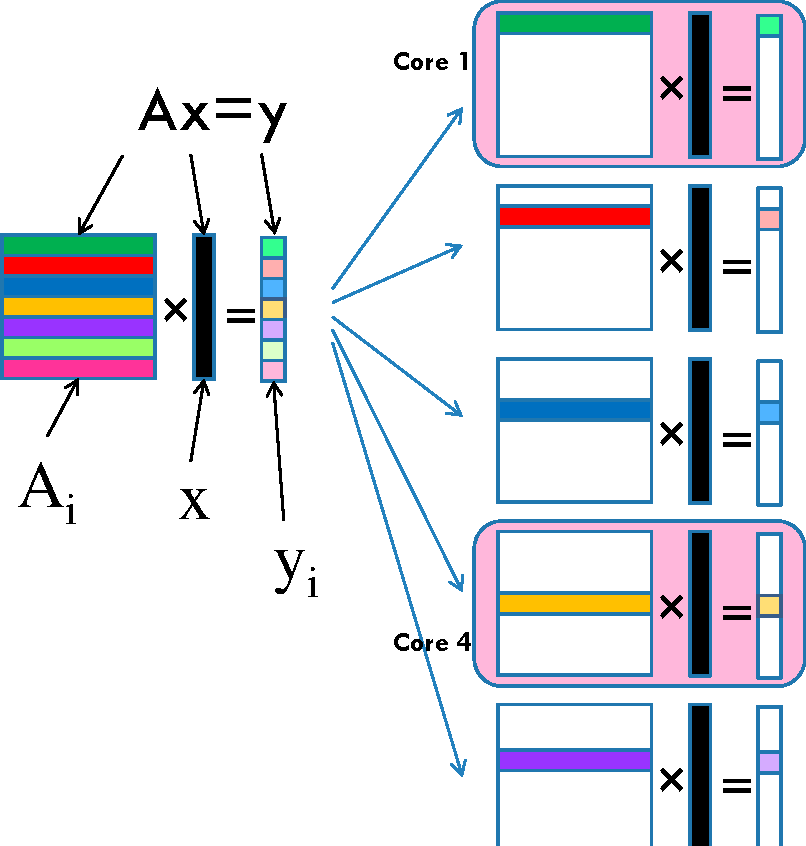
\includegraphics[width=.7\textwidth]{img/mvm-1.pdf}
    \caption{Example of MVM algorithm.}
\end{figure}

\newpage

\noindent
The performance of the MVM algorithm is as follows:
\begin{itemize}
    \item The \textbf{time to solve} a problem of size $n^{2}$ is equal to the big $O$ of the squared size of the problem as input divided by the number of processors available:
    \begin{equation*}
        T_{p}\left(n^{2}\right) = O\left(\dfrac{n^{2}}{p}\right)
    \end{equation*}
    
    \item The \textbf{cost} is equal to the number of processors and the time it takes to solve the problem. So it is quite trivial:
    \begin{equation*}
        C = O\left(\cancel{P} \cdot \dfrac{n^{2}}{\cancel{p}}\right) = O\left(n^{2}\right)
    \end{equation*}

    \item The \textbf{work} is equal to the cost, and the \textbf{linear power} $P$ is equal to the ratio of work and time to solve the problem on $p$ processors:
    \begin{equation*}
        W = C \hspace{2em} \dfrac{W}{T_{p}} = P
    \end{equation*}

    \item The \textbf{perfect efficiency} is equal to:
    \begin{equation*}
        E_{p} = \dfrac{T_{1}}{pT_{p}} = \dfrac{n^{2}}{p\frac{n^{2}}{p}} = 1
    \end{equation*}
\end{itemize}
    \subsection{SPMD sum}

The \definition{Single Program Multiple Data (SPMD)} is a term that has been used to \textbf{describe computational models} for exploiting parallelism, where \textbf{multiple processors work together to execute a program to get results faster}.

\highspace
In this section, we will see an SPMD approach on a Parallel Random Access Machine (PRAM). We will introduce one of the most common and simple mathematical operations: the sum.

\highspace
The following pseudocode takes as \textbf{input an array} of size $n = 2^{k}$. In this case, $n$ is a power of 2 because it ensures that the array can be evenly divided at each step of the computation. The value $k$ is the number of iterations or levels of the summation process.
\begin{lstlisting}[mathescape=true, caption={Single Program Multiple Data (SPMD) sum}]
BEGIN
    GLOBAL READ (A $\leftarrow$ A(I))
    GLOBAL WRITE (A $\rightarrow$ B(I))
    FOR H = 1 : K
        IF $i \le n \div 2^{h}$ THEN BEGIN
            GLOBAL READ (X $\leftarrow$ B(2$i$ - 1))
            GLOBAL READ (Y $\leftarrow$ B(2$i$))
            Z := X + Y
            GLOBAL WRITE (Z $\rightarrow$ B($i$))
        END
    IF I = 1 THEN
        GLOBAL WRITE (Z $\rightarrow$ S)
END
\end{lstlisting}
\begin{itemize}
    \item First, read the entire input array \texttt{A} and copy the read data to another array \texttt{B}.
    
    \item Loop over \texttt{h} (\texttt{1 to k}). In each iteration, for each index $i$ less than or equal to $n \div 2^{h}$, read values from array \texttt{B} at positions $2i-1$ and $2i$; sum these values (and store the result in \texttt{Z}) and store the result (\texttt{Z}) back into \texttt{B($i$)}.
    
    \item Once all iterations are complete, the final sum is stored in a variable \texttt{S}.
\end{itemize}
For example, if $n = 8$, then $k$ would be 3, meaning that the algorithm will run for 3 iterations to sum all the elements in parallel.
\begin{table}[!htp]
    \centering
    \begin{tabular}{@{} c c c @{}}
        \toprule
        $h$ & $i$ & adding \\
        \midrule
        \multirow{4}{*}{1} & 1 & 1,2 \\
          & 2 & 3,4 \\
          & 3 & 5,6 \\
          & 4 & 7,8 \\
        \cmidrule{1-3}
        \multirow{2}{*}{2} & 1 & 1,2 \\
          & 2 & 3,4 \\
        \cmidrule{1-3}
        3 & 1 & 1,2 \\
        \bottomrule
    \end{tabular}
\end{table}

\newpage

\begin{figure}[!htp]
    \centering
    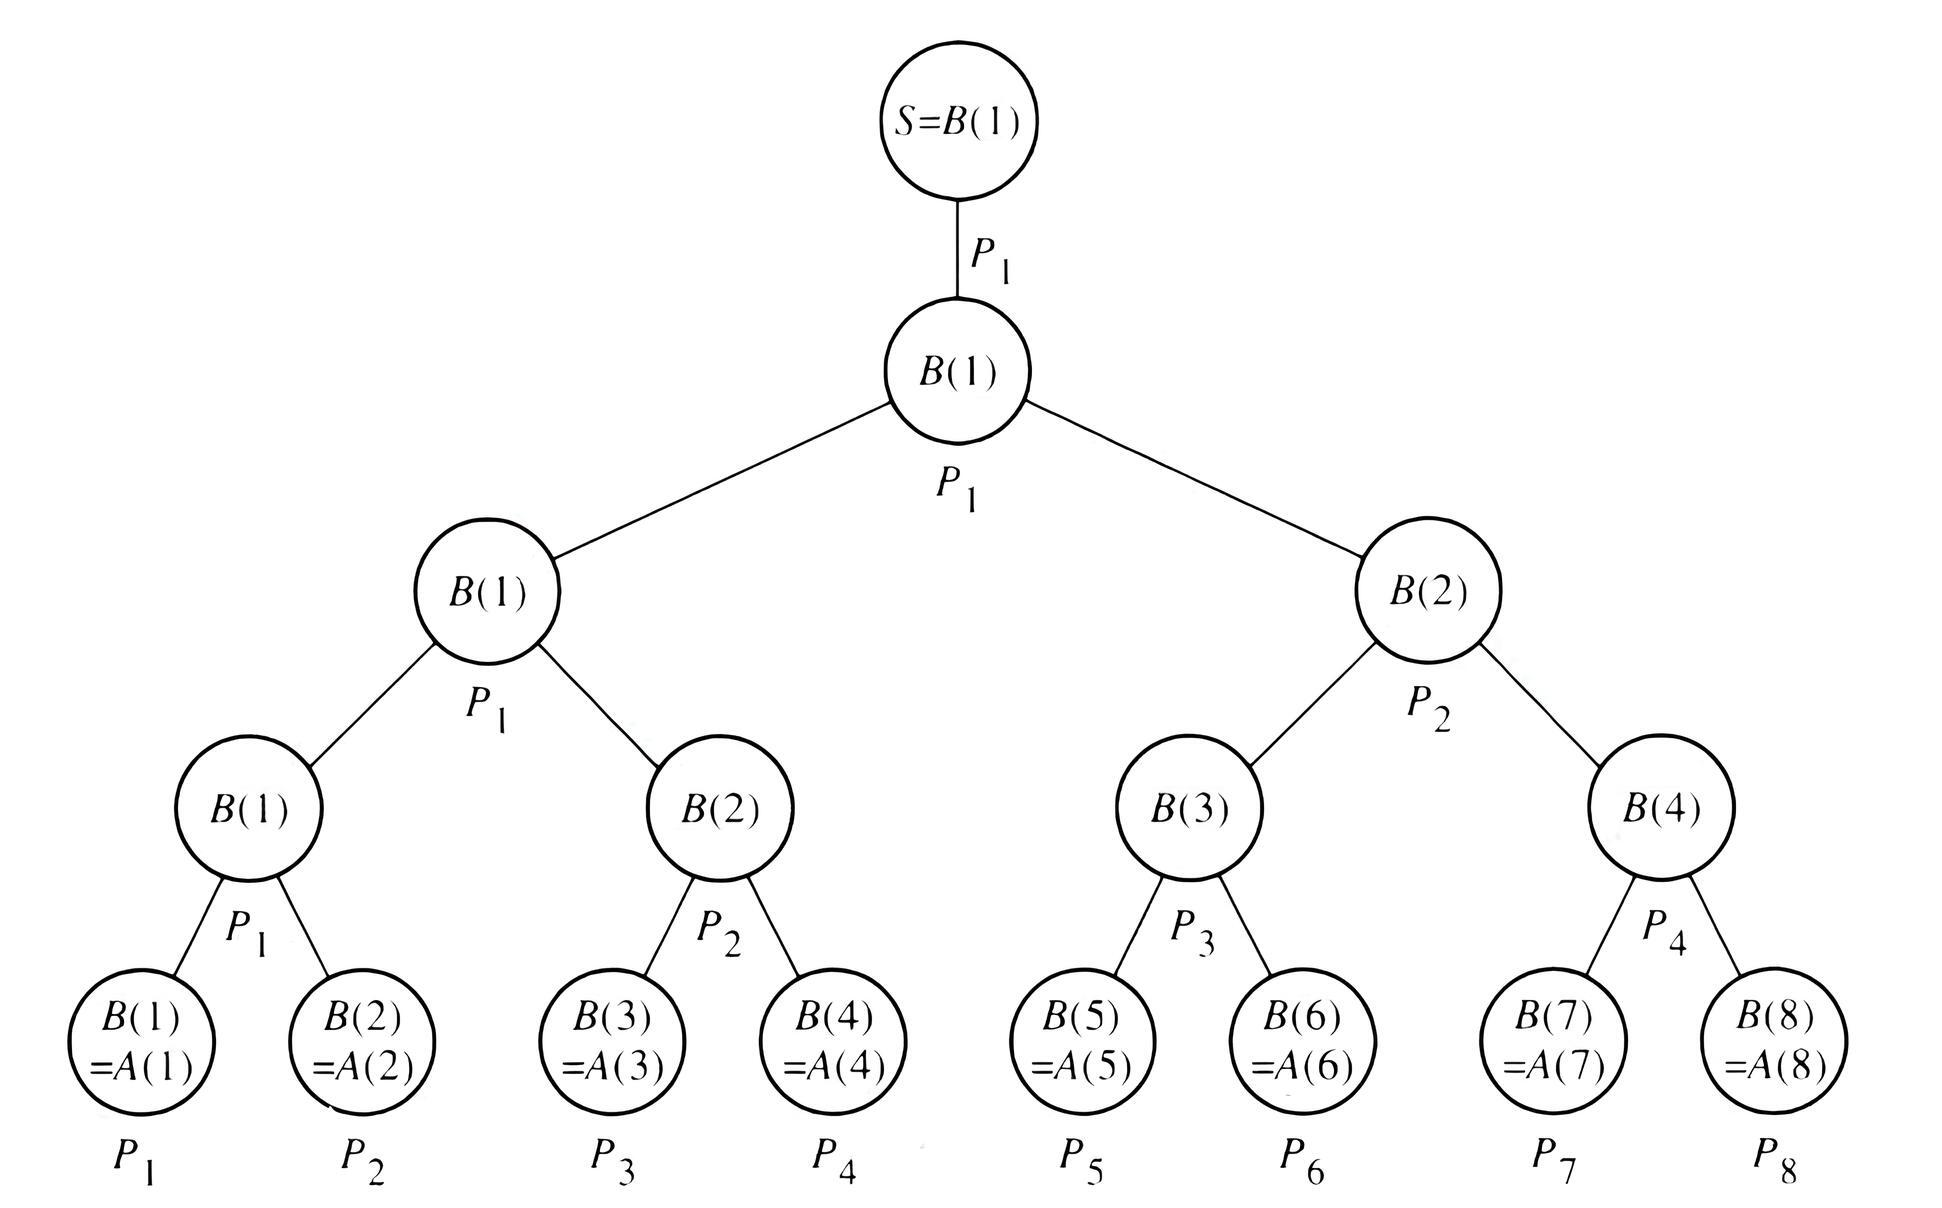
\includegraphics[width=\textwidth]{img/SPDM-sum-1.jpg}
    \caption{Computation of the sum of eight elements on a PRAM with eight processors. Each internal node represents a sum operation. The specific processor executing the operation is indicated below each node.}
    \label{fig: SPDM-sum-1}
\end{figure}

\begin{flushleft}
    \textcolor{Green3}{\faIcon{tachometer-alt} \textbf{Performance of sum}}
\end{flushleft}
When the size of the array is equal to the number of processors ($N = P$), the \textbf{speedup and efficiency decrease}:
\begin{itemize}
    \item $T^{*}\left(N\right) = T_{1}\left(N\right) = N$
    \item $T_{N=P}\left(N\right) = 2 + \log N$
    \item $\mathrm{SU}_{P} = \dfrac{N}{2+\log N}$
    \item $T^{*}\left(N\right) = P \cdot \left(2 + \log N\right) \approx N \log N$
    \item $E_{p} = \dfrac{T_{1}}{pT_{p}} = \dfrac{N}{N \log N} = \dfrac{1}{\log N}$
\end{itemize}
\begin{figure}[!htp]
    \centering
    \begin{subfigure}[h]{0.45\linewidth}
        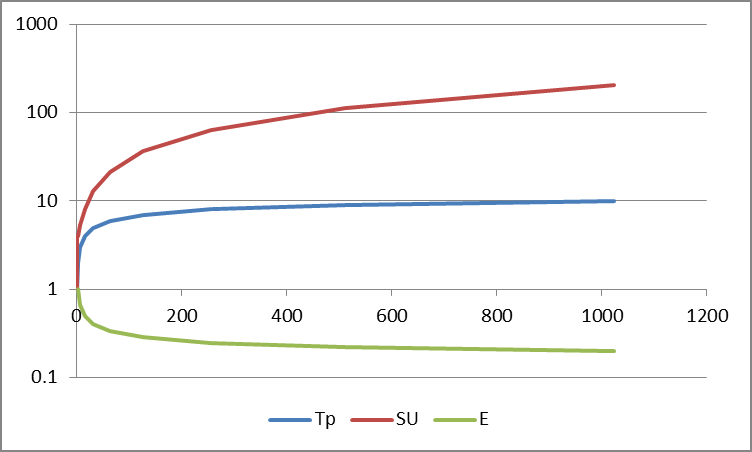
\includegraphics[width=\linewidth]{img/SPDM-sum-2.png}
    \end{subfigure}
    \hfill
    \begin{subfigure}[h]{0.45\linewidth}
        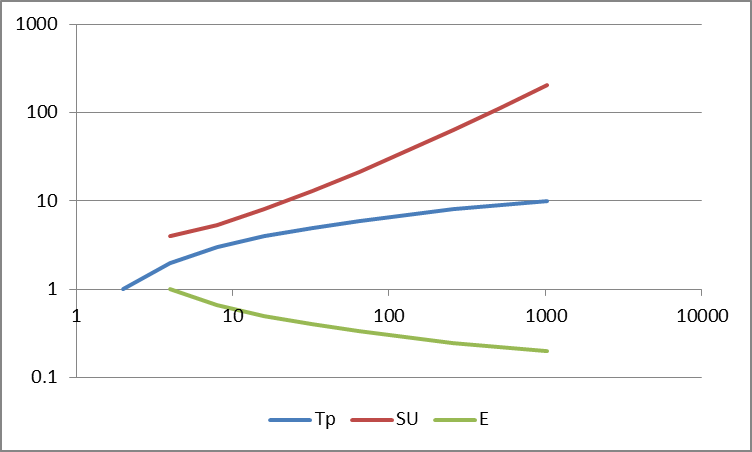
\includegraphics[width=\linewidth]{img/SPDM-sum-3.png}
    \end{subfigure}
\end{figure}

\newpage

\noindent
If the size of the array is much larger than the number of processors ($N \gg P$), the \textbf{speedup and power are linear}, the \textbf{cost is fixed} and the \textbf{efficiency is maximum (equal to 1)}:
\begin{itemize}
    \item $T^{*}\left(N\right) = T_{1}\left(N\right) = N$
    \item $T_{p}\left(N\right) = \dfrac{N}{p} + \log p$
    \item $\mathrm{SU}_{P} = \dfrac{N}{\frac{N}{p}+\log p} \approx P$
    \item $\text{COST} = p\left(\dfrac{N}{p} + \log p\right) \approx N$
    \item $\text{WORK} = N + P \approx N$
    \item $E_{p} = \dfrac{T_{1}}{pT_{p}} = \dfrac{N}{p\left(\frac{N}{p} + \log p\right)} \approx 1$
\end{itemize}
\begin{figure}[!htp]
    \centering
    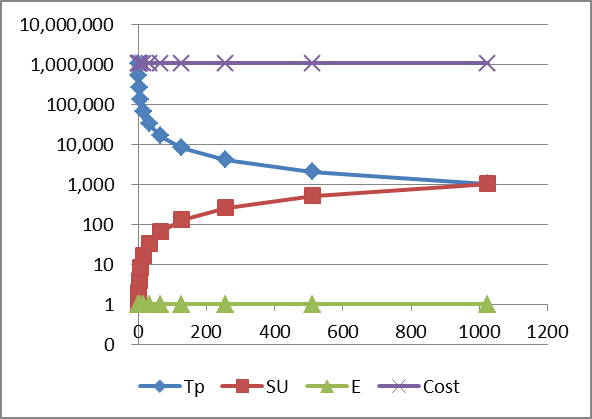
\includegraphics[width=.5\linewidth]{img/SPDM-sum-4.png}
    \caption*{$n = 1'000'000$}
\end{figure}

\begin{examplebox}
    Refer to Figure \ref{fig: SPDM-sum-1} (page \pageref{fig: SPDM-sum-1}), the performance metrics are:
    \begin{itemize}
        \item $T_{8} = 5$
        \item $C = 8 \cdot 5 = 40$ (could do 40 steps)
        \item $W = 2n = 16$ (16 on 40, wasted 24)
        \item $E_{p} = \dfrac{2}{\log n} = \dfrac{2}{3} = 0.67$
        \item $\dfrac{W}{C} = \dfrac{16}{40} = 0.4$
    \end{itemize}
\end{examplebox}
    \subsection{MM algorithm}

The \definition{Matrix Multiply (MM) algorithm} consists of three steps:
\begin{enumerate}
    \item \textbf{Compute the two matrices} $A_{i,l}$ and $B_{l,j}$, so use the concurrent read.
    \item Make the \textbf{sum}.
    \item \textbf{Store} the result using exclusive write.
\end{enumerate}
\begin{lstlisting}[mathescape=true, caption={Matrix Multiply (MM)}]
BEGIN
    $T_{i,j,l}$ = $A_{i,l} B_{l,j}$
    FOR = H = 1 : K
        IF $l \le n \div 2^{h}$ THEN
            $T_{i,j,l}$ = $T_{i,j,2l-1}$ + $T_{i,j,2l}$
    IF $l = 1$ THEN
        $C_{i,j}$ = $T_{i,j,1}$
END
\end{lstlisting}
\begin{flushleft}
    \textcolor{Green3}{\faIcon{tachometer-alt} \textbf{Performance of MM}}
\end{flushleft}
\begin{itemize}
    \item $T_{1} = n^{3}$
    \item $T_{p = n^{3}} = \log n$
    \item $\mathrm{SU} = \dfrac{n^{3}}{\log n}$
    \item $\text{Cost} = n^{3} \log n$
    \item $E_{p} = \dfrac{T_{1}}{pT_{p}} = \dfrac{1}{\log n}$
\end{itemize}
\begin{figure}[!htp]
    \centering
    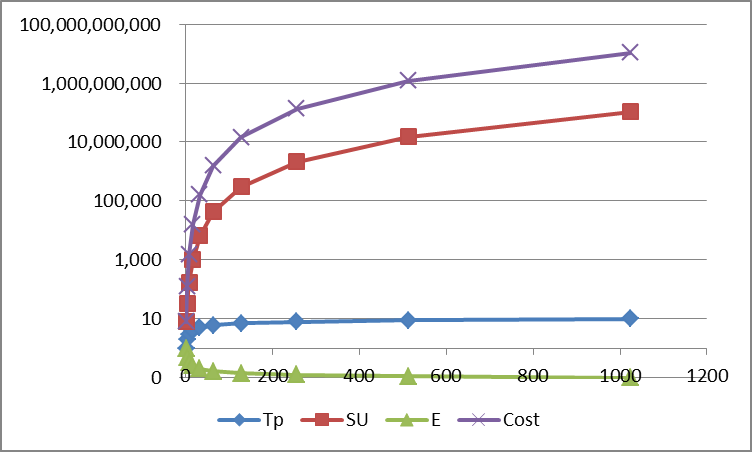
\includegraphics[width=.6\textwidth]{img/mm-1.png}
\end{figure}
    \subsection{PRAM variants and Lemmas}

The PRAM model presented here is one of the most commonly used. However, there are other important variants:
\begin{itemize}
    \item PRAM model with a \textbf{limited number of shared memory cells} (small memory PRAM). If the input data set exceeds the capacity of the shared memory, the I/O values can be evenly distributed among the processors.
    
    \item PRAM model with \textbf{limited number of processors} (small PRAM). If the number of execution threads is higher, processors can interleave multiple threads.

    \item PRAM model with \textbf{limited size of one machine word}.
    
    \item PRAM model with \textbf{access conflicts handling}. These are restrictions on simultaneous access to shared memory cells.
\end{itemize}

\begin{lemma}
    Assume $P' < P$ and same size of shared memory. Any problem that can be solved for a $P$ processor PRAM in $T$ steps can be solved in a $P'$ processor PRAM in:
    \begin{equation}
        T' = O\left(\dfrac{TP}{P'}\right)
    \end{equation}
\end{lemma}
\begin{proof}
    Partition $P$ is simulated processors into $P'$ groups of size $\frac{P}{P'}$ each. Associate each of the $P'$ simulating processors with one of these groups. Each of the simulating processors simulates one step of its group of processors by:
    \begin{itemize}
        \item Executing all their read and local computation substeps first;
        \item Executing their write substeps then.
    \end{itemize}
\end{proof}

\highspace
\begin{lemma}
    Assume $M' < M$. Any problem that can be solved for a $P$ processor and $M$-cell PRAM in $T$ steps can be solved on a $\max\left(P, M'\right)$-processors $M'$-cell PRAM in $O\left(\dfrac{TM}{M'}\right)$ steps.
\end{lemma}
\begin{proof}
    Partition $M$ simulated shared memory cells into $M'$ continuous segments $S$, of size $\frac{M}{M'}$ each. Each simulating processor $P_{I}'$ ($1 \le I \le P$), will simulate processor $P_{I}$ of the original PRAM. Each simulating processor $P_{I}'$ ($1 \le I \le M'$), stores the initial contents of $S_{I}$ into its local memory and will use $M'\left[I\right]$ as an auxiliary memory cell for simulation of accesses to cell of $S_{I}$.

    \noindent
    Simulation of one original read operation:
    \begin{lstlisting}[mathescape=true]
EACH $P_{I}'$ $\left(I = 1, \dots, \max\left(P, M'\right)\right)$ REPEATS FOR K = 1, ..., $\frac{M}{M'}$
    WRITE THE VALUE OF THE K-TH CELL OF $S_{I}$ INTO $M'\left[I\right]$ $\left(I = 1, \dots, M'\right)$
    READ THE VALUE WHICH THE SIMULATED PROCESSOR $P_{I}$ $\left(I = 1, \dots, P\right)$ WOULD READ IN THIS SIMULATED SUBSTEP, IF IT APPEARED IN THE SHARED MEMORY\end{lstlisting}
    The local computation substep of $P_{I}$ ($I = 1, \dots, P$) is simulated in one step by $P_{I}'$. SImulation of one original write operation is analogous to that of read.
\end{proof}

    \subsection{PRAM implementation}

The PRAM is an ideal model for creating parallel algorithms. Now we look at \dquotes{\emph{is it really implementable?}} The short answer is yes.

\highspace
The longest answer is the following. There are already some examples of PRAM being converted to real machine models, such as \href{https://en.wikipedia.org/wiki/Explicit_multi-threading}{Explicit Multi-Threading \break (XMT)}, Rigel, Tilera, etc. If conversion is not easy or possible, the implementation can be \dquotes{\emph{direct}}:
\begin{itemize}
    \item The concurrent read is implemented as a detect-and-multicast technique.
    \item The concurrent write is implemented depending on the end result we want to achieve. Fetch-and-operate and prefix-sum are examples of serialized writing; otherwise, the CRCW technique is used:
    \begin{itemize}
        \item Common CRCW: detect and merge
        \item Priority CRCW: detect-and-priorities
        \item Arbitrary CRCW: arbitrary
    \end{itemize}
\end{itemize}

\begin{examplebox}[: Boolean DNF (sum of products) common CRCW]
    A logical formula is considered to be in DNF if it is a disjunction of one or more conjunctions of one or more literals.

    Consider $X$ as the sum of products of AND/OR operations:
    \begin{equation*}
        X = a_{1}b_{1} + a_{2}b_{2} + \dots
    \end{equation*}
    The PRAM code, with $X$ initialized to $0$ and task index equal to \$, is:
    \begin{center}
        \texttt{if ($a_{\$}b_{\$}$) X = 1;}
    \end{center}
    The common result is that not all processors write $X$ and those that do write 1. The time complexity is $O\left(1\right)$. It works on common, priority and arbitrary CRCW.
\end{examplebox}

\noindent
Despite the previous example, exists also the PRAM SoP for the concurrent write. Let boolean $X$ as:
\begin{equation*}
    X = a_{1}b_{1} + a_{2}b_{2} + \dots
\end{equation*}
The PRAM algorithm is:
\begin{center}
    \texttt{if ($a_{i}b_{i}$) X = 1;}
\end{center}
Where all cores which write into $X$, \textbf{write the same value}.

\newpage

\begin{flushleft}
    \textcolor{Green3}{\faIcon{check} \textbf{PRAM advantages}}
\end{flushleft}
\begin{itemize}
    \item Large body of algorithms.
    \item Easy to think about it.
    \item Sync version of shared memory. It eliminates sync and common issues, allows focus on algorithms, but allows adding these issues and allows conversion to async versions.
    \item Exists architectures for both synch (PRAM) and async (SM) model.
    \item PRAM algorithms can be mapped to other models.
\end{itemize}
    \subsection{Amdahl's and Gustafson's Laws}

The \definition{Amdahl's Law} is a formula which gives the \textbf{theoretical speedup in latency of the execution of a task at fixed workload that can be expected of a system whose resources are improved}. The law can be stated as:
\begin{definitionbox}[: Amdahl's Law]
    \textbf{The overall performance improvement gained by optimizing a single part of a system is limited by the fraction of time that the improved part is actually used.}
\end{definitionbox}

\noindent
In practice, Amdahl's law says that the computation consists of interleaved segments of two types:
\begin{enumerate}
    \item \textbf{Serial segments} (which cannot be parallelized);
    \item \textbf{Parallelizable segments}.
\end{enumerate}
Therefore, the metrics we can obtain are the time on $P$ processors metric, that it is greater than the fraction of time on a processor divided by the processors $P$, and the speedup metric, that it is less than the number of processors $P$:
\begin{equation*}
    T_{P} > \dfrac{T_{1}}{P} \hspace{2em} SU < P
\end{equation*}
Graphically, we can see a fixed part of the line, which is the \textbf{serial segment} (no speedup), and a set of instructions that can be \textbf{parallelized} (the sum of these segments is equal to the unit time $1$).
\begin{figure}[!htp]
    \centering
    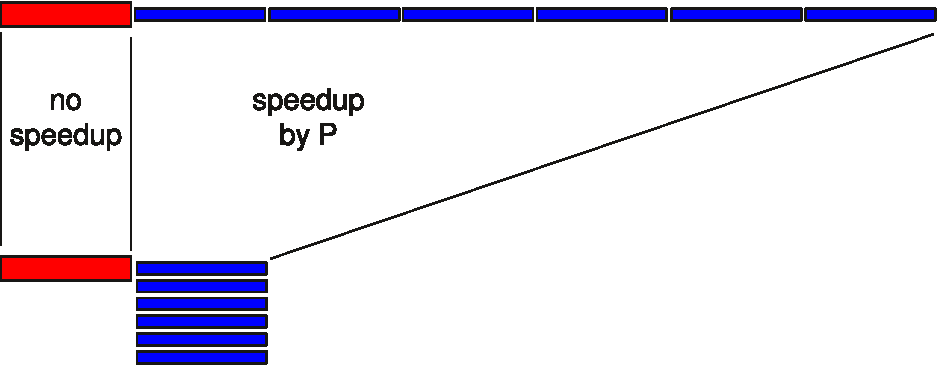
\includegraphics[width=\textwidth]{img/amdahl-law-1.pdf}
\end{figure}

\noindent
Furthermore, if we identify the parallelizable segment as $f$ and the serial segment as $1-f$, we obtain the following expressions:
\begin{equation}
    \begin{array}{rcl}
        SU\left(P,f\right) &=& \dfrac{T_{1}}{T_{P}} = \dfrac{T_{1}}{T_{1} \cdot \left(1-f\right) + \frac{T_{1}\cdot f}{P}} = \dfrac{1}{\left(1-f\right) + \frac{f}{P}} \\ [1em]
        \lim\limits_{P \rightarrow \infty}SU\left(P,f\right) &=& \dfrac{1}{1-f}
    \end{array}
\end{equation}

\highspace
In the following figure we can see the speedup with parameter $f$. Note the pessimism: for a problem with inherent $f=90\%$, there is no point in using more than 10 processors.
\begin{figure}[!htp]
    \centering
    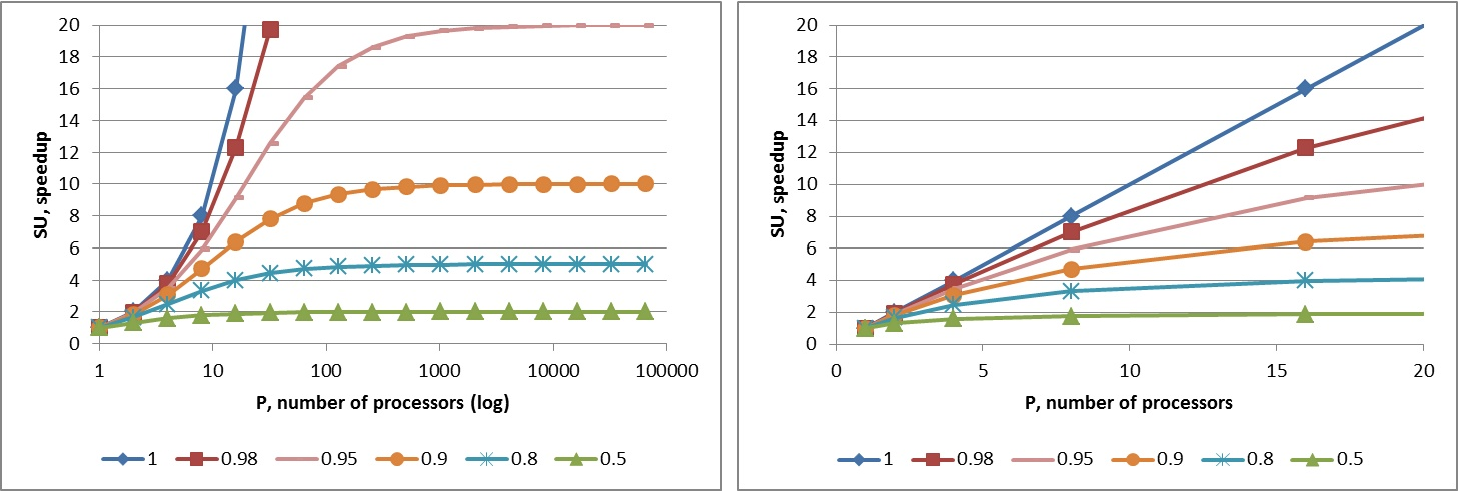
\includegraphics[width=\textwidth]{img/amdahl-law-2.pdf}
    \caption{Amdahl's law, $SU\left(P\right)$, parameter $f$.}
\end{figure}

\noindent
The original paper presenting Amdahl's Law\cite{amdahl2007validity} can be viewed by clicking on the link below or by scanning the QR code.
\begin{center}
    \href{https://ieeexplore.ieee.org/abstract/document/4785615}{Amdahl's Law}
    \hspace{2em}
    \qrcode{https://ieeexplore.ieee.org/abstract/document/4785615}
\end{center}
\textbf{Amdahl's law applies only to the cases where the problem size is fixed}. In practice, as more computing resources become available, they tend to get used on larger problems (larger datasets), and the time spent in the parallelizable part often grows much faster than the inherently serial work. In this case, \textbf{Gustafson's law gives a less pessimistic and more realistic assessment of the parallel performance}.\cite{mccool2012structured}

\highspace
\definition{Gustafson's Law} gives the speedup in the execution time of a task that theoretically gains from parallel computing, using a hypothetical run of the task on a single-core machine as the baseline. To put it another way, it is the \textbf{theoretical \dquotes{slowdown} of an already parallelized task if running on a serial machine}.

\highspace
Against Amdahl's law, Gustafson suggests the following ideas:
\begin{itemize}
    \item Portion $f$ is not fixed;
    \item The absolute serial time is fixed;
    \item Parallel problem size is increased to exploit more processors;
    \item Fixed serial time ($s$ of total) and fixed parallel time ($1-s$ of total) are invariants;
    \item \textbf{Fixed time model} and not fixed size model (as Amdahl's law):
    \begin{equation}
        SU\left(P\right) = \dfrac{T_{1}}{T_{P}} = \dfrac{s+P\cdot\left(1-s\right)}{s+\left(1-s\right)} = s + P\cdot\left(1-s\right)
    \end{equation}
\end{itemize}

\newpage

\noindent
Gustafson's law suggests a \textbf{linear speedup} and is \textbf{empirically applicable to highly parallel algorithms}.
\begin{figure}[!htp]
    \centering
    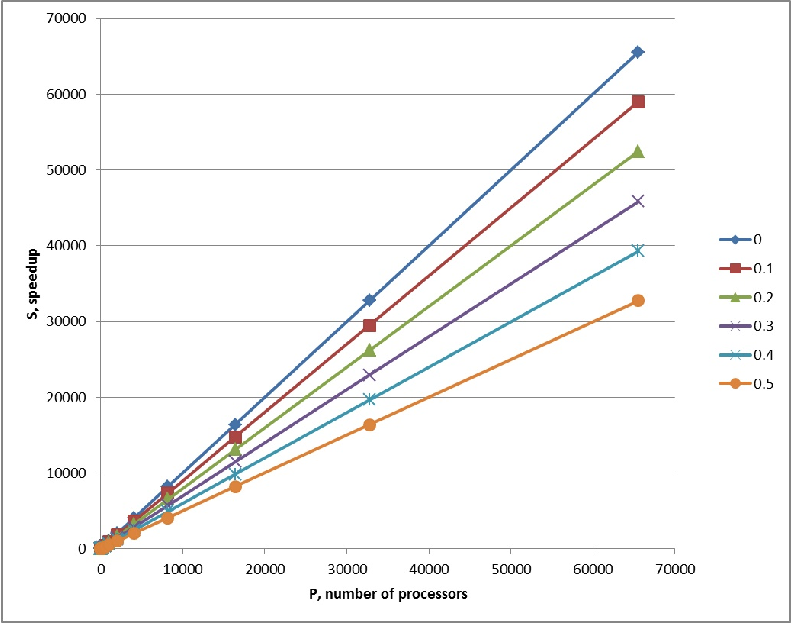
\includegraphics[width=.7\textwidth]{img/gustafson-law-1.pdf}
    \caption{Gustafson's law.}
\end{figure}

\noindent
\textbf{\emph{Amdahl's Law}} states that as computing power increases, computational requirements remain the same. In other words, the \textbf{analysis of the same data will take less time with more computing power}.

\textbf{\emph{Gustafson}}, on the other hand, argues that \textbf{more computing power leads to more careful and complete analysis of the data}. Where it would not have been possible or practical to simulate the impact of nuclear denotation on every building, car, and their contents (including furniture, structural strength, etc.) because such a calculation would have taken more time than was available to provide an answer, the increase in computing power will prompt researchers to add more data to more fully simulate more variables, giving a more accurate result.

\highspace
The original paper presenting Gustafson's Law\cite{gustafson1988reevaluating} can be viewed by clicking on the link below or by scanning the QR code.
\begin{center}
    \href{https://dl.acm.org/doi/abs/10.1145/42411.42415}{Gustafson's Law}
    \hspace{2em}
    \qrcode{https://dl.acm.org/doi/abs/10.1145/42411.42415}
\end{center}

    %%%%%%%%%%%%%%%%%%%%%%%%%%%%%%%%
    % Fundamentals of architecture %
    %%%%%%%%%%%%%%%%%%%%%%%%%%%%%%%%
    \section{Fundamentals of architecture}

\subsection{Introduction}

\subsubsection{Simplest processor}

Inside a computer, a processor executes instructions.
\begin{itemize}
    \item \textbf{Fetch/Decode}: Determine which instruction to run next;
    \item \textbf{ALU} (execution unit): Performs the operation described by an instruction, which may change values in the processor's registers or the computer's memory;
    \item \textbf{Registers}: maintain program state, store values of variables used as inputs and outputs to operations.
\end{itemize}
The simplest and most basic processor executes \textbf{one instruction per clock cycle}.
\begin{figure}[!htp]
    \centering
    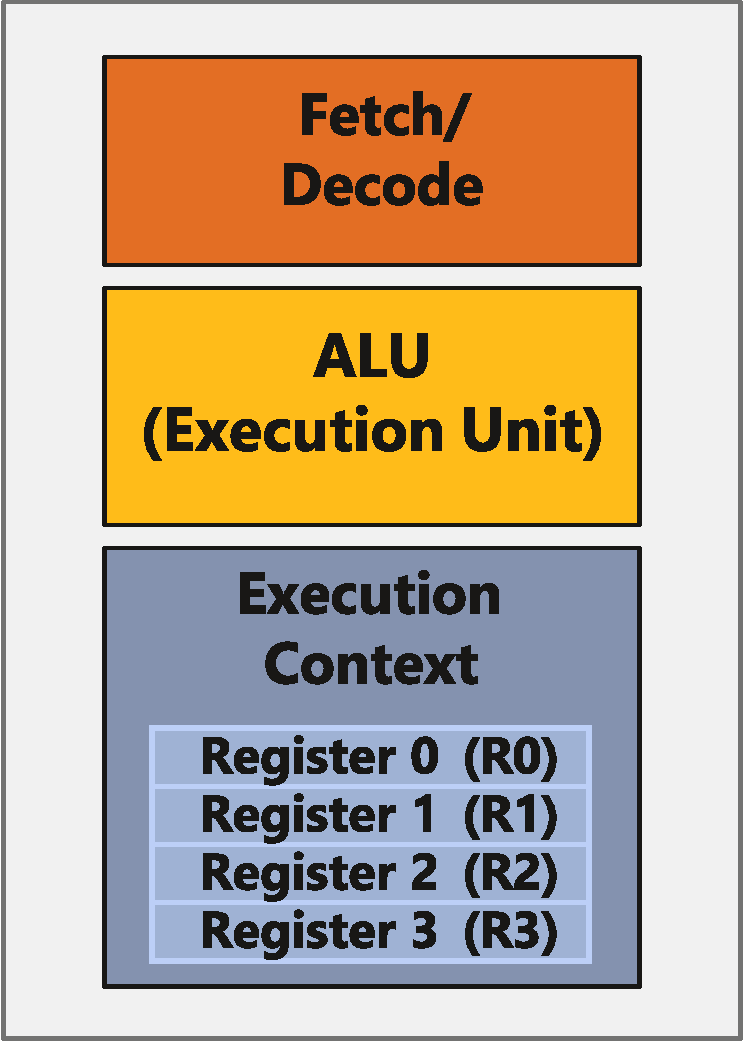
\includegraphics[width=.3\textwidth]{img/simplest-prcoessor-1.pdf}
    \caption{The simplest and most basic processor.}
\end{figure}

\newpage

\subsubsection{Superscalar processor}
A more \dquotes{complex} and realistic model is the \definitionWithSpecificIndex{superscalar processor}{Superscalar Processor}. This \textbf{processor can decode and execute up to \underline{two instructions per clock}}. The execution is slightly different from the simplest processor. The \textbf{processor automatically finds independent instructions in an instruction sequence and can execute them in parallel on multiple execution units}.
\begin{figure}[!htp]
    \centering
    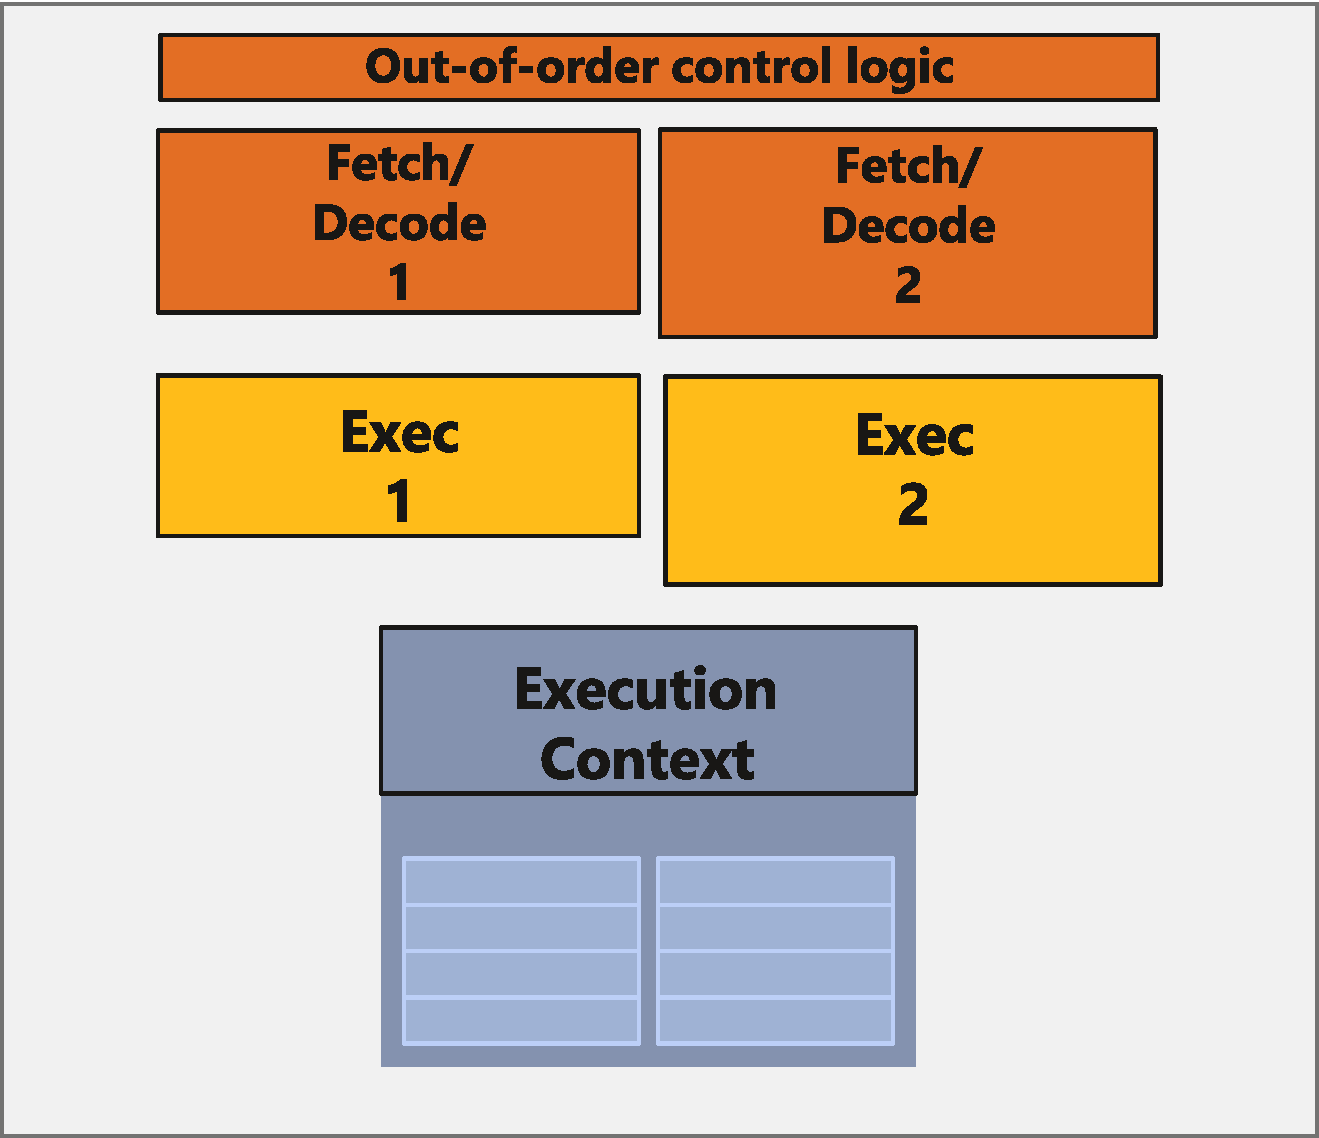
\includegraphics[width=.52\textwidth]{img/superscalar-prcoessor-1.pdf}
    \caption{The superscalar processor.}
\end{figure}

\noindent
The superscalar processor takes advantage of \definition{Instruction-Level Parallelism (ILP)}\footnote{Instruction-level parallelism (ILP) is the parallel or simultaneous execution of a sequence of instructions in a computer program. More specifically ILP refers to the average number of instructions run per step of this parallel execution.} within an instruction stream.
\begin{itemize}
    \item Processing \textbf{different instructions} from the same instruction stream \textbf{in parallel} (\textbf{within a core}).
    \item \textbf{Parallelism is automatically detected by the hardware during execution}.
\end{itemize}

\newpage

\subsubsection{Single Instruction, Multiple Data (SIMD) processor}

Adding execution units (ALUs) to the simplest processor can increase compute capability. Amortize the cost/complexity of managing an instruction stream across many ALUs using \definition{Single Instruction, Multiple Data (SIMD)} processing. Therefore, the \textbf{same instruction is sent to all ALUs}. This \textbf{operation is performed in parallel on all ALUs}.

\begin{flushleft}
    \textcolor{Green3}{\faIcon{check} \textbf{Advantages}}
\end{flushleft}
\begin{itemize}
    \item \textbf{Efficient for data-parallel workloads}: amortize control costs over many ALUs.
    \item Vectorization done by:
    \begin{itemize}
        \item Compiler (\textbf{\underline{explicit SIMD}}): parallelism is explicitly requested by the programmer through intrinsics, conveyed through parallel language semantics, and inferred through loop dependency analysis by the \dquotes{auto-vectorizing} compiler. In other words, the \textbf{SIMD parallelization is done at compile time, and when we inspect the program binary, we can see the SIMD instructions}.

        \item At runtime by hardware (\textbf{\underline{implicit SIMD}}): the \textbf{compiler generates a binary with scalar instructions}, but $n$ instances of the program are always executed together on the processor. The \textbf{hardware} (not the compiler) is \textbf{responsible for the simultaneous execution of the same instruction by multiple program instances on different data on SIMD ALUs}.
    \end{itemize}
\end{itemize}

\longline

\subsubsection{Multi-Core Processor}

A \definition{Multi-Core Processor (MCP)} is a \textbf{microprocessor} on a single integrated circuit (IC) with \textbf{two or more separate central processing units (CPUs)}, called \emph{cores} to emphasize their multiplicity (e.g., \emph{dual-core} or \emph{quad-core}). Each core reads and executes program instructions, specifically ordinary CPU instructions (such as \texttt{add}, \texttt{move data}, and \texttt{branch}). However, the MCP can \textbf{execute instructions on separate cores simultaneously}, \textbf{increasing overall speed for programs that support multithreading or other parallel computing techniques}.
\begin{flushleft}
    \textcolor{Green3}{\faIcon{check} \textbf{Advantages}}
\end{flushleft}
\begin{itemize}
    \item Provides \textbf{thread-level parallelism}: execute a completely different instruction stream on each core simultaneously.
    \item \textbf{Software creates threads to expose parallelism to hardware} (e.g., via threading API)
\end{itemize}
    \subsection{Accessing Memory}\label{subsection: Accessing Memory}

\subsubsection{What is a memory?}

A computer's memory is organized as an array of bytes. Each byte is identified by its address in memory (its position in that array).
\begin{table}[!htp]
    \centering
    \begin{tabular}{@{} c | c @{}}
        \toprule
        Address & Value \\
        \midrule
        \texttt{0x0} & \texttt{16} \\
        \texttt{0x1} & \texttt{255} \\
        \texttt{0x2} & \texttt{14} \\
        \texttt{0x3} & \texttt{0} \\
        \texttt{0x4} & \texttt{0} \\
        \texttt{0x5} & \texttt{0} \\
        \texttt{0x6} & \texttt{6} \\
        \texttt{0x7} & \texttt{0} \\
        \texttt{0x8} & \texttt{32} \\
        \texttt{0x9} & \texttt{48} \\
        \texttt{0xA} & \texttt{255} \\
        \texttt{0xB} & \texttt{255} \\
        \texttt{0xC} & \texttt{255} \\
        \texttt{0xD} & \texttt{0} \\
        \texttt{0xE} & \texttt{0} \\
        \texttt{0xF} & \texttt{0} \\
        \texttt{0x10} & \texttt{128} \\
        \vdots & \vdots \\
        \texttt{0x1F} & \texttt{0} \\
        \bottomrule
    \end{tabular}
    \caption{Example illustration of the program's memory address space of 32 bytes, range from \texttt{0x0} to \texttt{0x1F}.}
\end{table}

\noindent
From the processor's point of view, loading an instruction to access the contents present in memory is done with the \texttt{ld} assembly instruction. For example, \texttt{ld R0 $\leftarrow$ mem[R2]} means \dquotes{take the value from register \texttt{R2} and put that value into register \texttt{R0}}.

\highspace
Before we introduce new concepts, let us take a moment to explain some important \textbf{terminology}:
\begin{itemize}
    \item \definition{Memory Access Latency}, is the \textbf{time} it takes for the \textbf{memory system to deliver data to the processor}.
    
    \item \definition{Processor Stall}. A \textbf{processor} stalls when it \textbf{cannot execute the next instruction in an instruction stream because of a dependency on a previous instruction that has not been completed}. Accessing memory is a major source of stalling, which is one of the main reasons why memory accesses should be limited. 
    \newpage
    For \example{example}, in the following three assembler instructions, the add has to wait for the loading of \texttt{R2} and \texttt{R3} values, making parallelization more complicated:
    \begin{flushleft}
    	\texttt{ld r0 mem[r2]}\newline
    	\texttt{ld r1 mem[r3]}\newline
    	\texttt{add r0, r0, r1}
    \end{flushleft}
    
    \item \definition{Memory Bandwidth}, is the \textbf{rate at which the memory system can provide data to a processor}.

    Bandwidth is the \underline{critical} resource in modern computing.
    
    \textbf{High-performance parallel programs will}:
    \begin{enumerate}
        \item \textbf{Organize computation to fetch data from memory less frequently}. For example, reuse data previously loaded by the same thread (temporal locality optimizations) or share data across threads (inter-thread cooperation);
        
        \item Prefer to \textbf{perform additional arithmetic to store/reload values};
        
        \item \textbf{Programs need to access memory infrequently} to take advantage of modern processors.
    \end{enumerate}
\end{itemize}

\newpage

\subsubsection{How to reduce processor stalls}

\paragraph{Cache}

One of the most common solutions is caching.

\highspace
A \definitionWithSpecificIndex{cache}{Cache}{} is a hardware or software \textbf{component that stores data so that future requests for that data can be served faster}; the data stored in a cache might be the result of an earlier computation or a copy of data stored elsewhere.
\begin{itemize}
    \item A \definition{Cache Hit} occurs when the \textbf{requested data is found} in a cache;
    \item A \definition{Cache Miss} occurs when \textbf{it cannot}.
\end{itemize}
Cache hits are served by reading data from the cache, which is faster than recomputing a result or reading from a slower data store, so the \textbf{more requests that can be served from the cache, the faster the system performs}.\cite{wikipediaCacheResearch}

\highspace
Many modern CPUs have logic that predicts what data will be accessed in the future and \dquotes{pre-fetches} that data into caches. \definition{Prefetching} reduces stalls because the data is resident in the cache when it is accessed. But beware, the other side of the coin is that if the \textbf{guess is wrong}, the \textbf{performance is worse than the system without prefetching}!

\longline

\paragraph{Multi-threading}

A \definition{Multithreaded Processor} is one that has the \textbf{ability to follow multiple instruction streams without software intervention}. In practice, then, this \textbf{includes any machine that stores multiple program counters (PCs) in hardware within the processor} (i.e., on chip, for microprocessor-era machines).\cite{nemirovsky2022multithreading}

\highspace
The main idea in this architecture is to \textbf{interleave processing of multiple threads on the same core to hide stalls}. In other words, if we can't make progress on the current thread, we work on another one.

\begin{examplebox}[: core utilization]\label{example: core utilization}
    To better understand our explanation, suppose we are running a program where threads perform \textbf{three arithmetic instructions followed by a memory load} (with 12 cycle latency).
    \begin{center}
        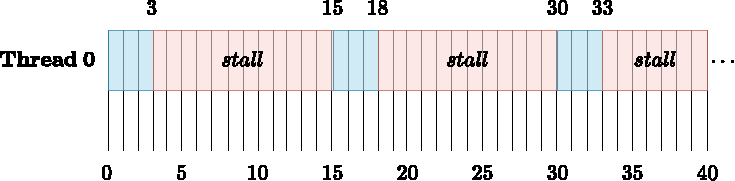
\includegraphics[width=\textwidth]{img/multi-threading-1.pdf}
    \end{center}

    From the figure, it is clear that if we consider an arithmetic instruction and a memory stall, the core is not fully optimized to work at 100\%. In practice, we see that a single arithmetic instruction takes 3 clock cycles and the memory stall takes 12 clock cycles. This means that from this situation we are using the CPU at only 20\% (3 work clock cycles on 15)!

    Without suggesting the final solution, try to see what happens when we add another thread.
    \begin{center}
        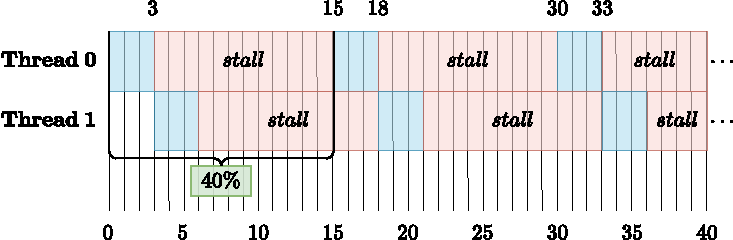
\includegraphics[width=\textwidth]{img/multi-threading-2.pdf}
    \end{center}
    
    We have gained three clock cycles, and now we are taking advantage of the 40\% of the core.

    Now, how many threads do we need to achieve 100\% utilization? The answer is simple: the number of clock cycles of the operations to be done before the stall plus the clock cycles of the stall divided by the working operations (operations that are not stalls). In our case: $15 \div 3 = 5$.
    \begin{center}
        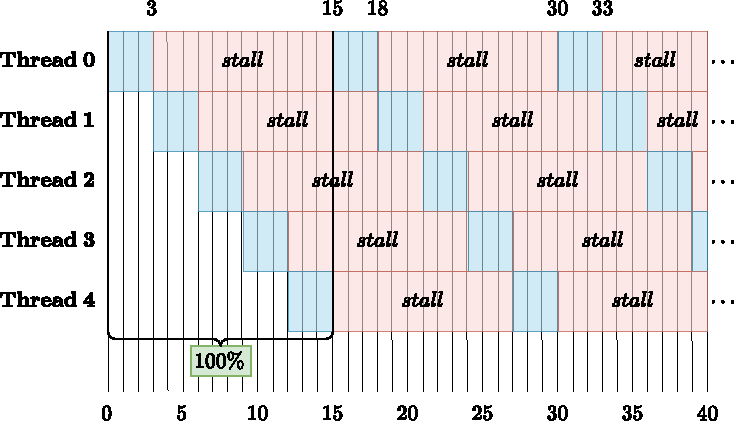
\includegraphics[width=\textwidth]{img/multi-threading-3.pdf}
    \end{center}

    Note that if we add more threads, there will be no benefit because the CPU is already at 100\%.
\end{examplebox}

\begin{flushleft}
    \textcolor{Green3}{\faIcon{check} \textbf{Multithreaded Processor benefits}}
\end{flushleft}
\begin{itemize}
    \item A processor with multiple hardware threads has the \textbf{ability to avoid stalls} by executing instructions from other threads when one thread must wait for a long latency operation to complete. The latency of the memory operation is not changed by multithreading, it just no longer causes reduced processor utilization.
    
    \item A \textbf{multithreaded processor hides memory latency by performing arithmetic from other threads}. Program that feature more arithmetic per memory access need fewer threads to hide memory stalls.
\end{itemize}

\begin{flushleft}
    \textcolor{Red2}{\faIcon{microchip} \textbf{Type of hardware-supported multithreading}}
\end{flushleft}
\begin{itemize}
    \item \textbf{Core manages execution contexts for multiple threads}. This type still has the same number of ALU resources: multi-threading only helps to use them more efficiently in the face of high latency operations such as memory access. The \textbf{processor decides which thread to run each clock cycle}.
    
    \item \definition{Coarse-Grain Multithreading}, also called \blackdefinition{Block Multithreading} or \blackdefinition{Switch-On-Event Multithreading}, has multiple hardware contexts associated  with each processor core. A hardware context is the program counter, register file, and other data required to enabled a software thread to execute on a core. However, only one hardware context has access to the pipeline at a time.\cite{nemirovsky2022multithreading}

    \item \definition{Fine-Grain Multithreading (FGMT)}, also known as \blackdefinition{Interleaved Multithreading} or \blackdefinition{Temporal Multithreading}, is the type just described on the previous pages, as in the example on page \pageref{example: core utilization}.

    \item \definition{Simultaneous Multithreading (SMT)} has multiple hardware contexts associated with each core. In a simultaneous multithreaded processor, instructions from multiple threads are available to be issued on any cycle. Therefore, all hardware contexts, and in particular all register files, must be accessible to the pipeline and its execution resources.\cite{nemirovsky2022multithreading}
    
    In other words, \textbf{each clock}, the \textbf{core selects instructions from multiple threads to execute on ALUs}.
\end{itemize}

    %%%%%%%%%%%%%%%%%%%%%%
    % Programming models %
    %%%%%%%%%%%%%%%%%%%%%%
    \section{Programming models}

\subsection{Implicit SPMD Program Compiler (ISPC)}

Before introducing the ISPC compiler, we give the definition of SPMD.

\begin{definitionbox}[: Single Program, Multiple Data (SPMD)]
    \definition{Single Program, Multiple Data (SPMD)} is a term that has been used to refer to computational models for exploiting parallelism, where \textbf{multiple processors work together to execute a program to achieve faster results}.

    The \textbf{difference} between \emph{SPMD} and \emph{SIMD} (page \pageref{subsubsection: Single Instruction, Multiple Data (SIMD) processor}) is that in SPMD parallel execution, \textbf{multiple autonomous processors simultaneously execute the same program at independent points}, rather than in SIMD it is vectorization at the instruction level so that \textbf{each CPU instruction processes multiple data elements}.

    In other words:
    \begin{itemize}
        \item SPMD: is the \textbf{programming abstraction}, because the programmer has to think; the program is written in terms of this abstraction.
        \item SIMD: in general, the compilers (ISPC) issue special vector instructions that execute the logic performed by each parallel instance created (ISPC gang spawned). In addition, the compilers handle the mapping of conditional control flow to vector instructions.
    \end{itemize}
    The difference and the terminology used by ISPC will become clearer in the following pages. We suggest that finish this section and come back here in a moment.
\end{definitionbox}

\begin{definitionbox}[: Implicit SPMD Program Compiler (ISPC)]
    \definition{Implicit SPMD Program Compiler (ISPC)} is a \textbf{compiler for a variant of the C programming language}, with extensions for \emph{Single Program, Multiple Data (SPMD)} programming. Under the SPMD model, the programmer writes a program that generally appears to be a regular serial program, though the execution model is actually that a number of program instances execute in parallel on the hardware. In other words, the \textbf{ISPC gives the programmer some API to do parallelization on the code; it also generates high quality SIMD code to increase performance}.
\end{definitionbox}

\noindent
The definition, implementation, and other details are explained in the official \href{https://github.com/ispc/ispc}{Intel GitHub repository}.

\newpage

\begin{flushleft}
    \textcolor{Green3}{\faIcon{question-circle} \textbf{How it works?}}
\end{flushleft}
Let us take a general main program; when we call an \texttt{ispc} function, it causes a \textbf{spawn of gang of ISPC program instances upon return, all instances have completed}. These \textbf{instances execute the same ISPC code simultaneously}, and \textbf{each instance has its own copy of local variables}. Take the following ISPC code as an example:
\begin{lstlisting}[language=c++, mathescape]
export void ispc_sinx(
    uniform int N, $\label{code: uniform}$
    uniform int terms,
    uniform float* x,
    uniform float* result
){
    // assume N % programCount = 0
    for (uniform int i=0; i<N; i+=programCount) { $\label{code: programCount}$
        int idx = i + programIndex; $\label{code: programIndex}$
        float value = x[idx];
        float numer = x[idx] * x[idx] * x[idx];
        uniform int denom = 6; // 3!
        uniform int sign = -1;
        for (uniform int j=1; j<=terms; j++) { 
            value += sign * numer / denom
            numer *= x[idx] * x[idx];
            denom *= (2*j+2) * (2*j+3);
            sign *= -1;
        }
        result[idx] = value;
    }
}
\end{lstlisting}
In the example, the \texttt{programCount} (row \ref{code: programCount}) and \texttt{programIndex} (row \ref{code: programIndex}) variables, \texttt{uniform} (row \ref{code: uniform}, and so on) data type tell us:
\begin{itemize}
    \item \texttt{programIndex} gives the index of the SIMD-lane being used for running each program instance (in other words, it's a varying \textbf{integer value that has value zero for the first program instance, and so forth}).
    
    \item \texttt{programCount} gives the \textbf{total number of instances in the \emph{gang}}.
    
    \item A variable that is declared with the \texttt{uniform} qualifier represents a \textbf{single value that is shared across the entire \emph{gang}}. 
\end{itemize}
Together, these can be used to uniquely map executing program instances to input data (\href{https://ispc.github.io/ispc.html#parallel-iteration-with-programindex-and-programcount}{programIndex and programCount}, \href{https://ispc.github.io/ispc.html#uniform-data}{uniform data type}).

\highspace
With the ISPC analogy, the \definition{SPMD programming model} should be clear:
\begin{enumerate}
    \item \textbf{Single thread of control} (typically a main program);
    \item \textbf{Invoke} the \textbf{SPMD function} (in the previous example, the \texttt{ispc\_sinx} function);
    \item \textbf{SPMD execution}, then \textbf{multiple instances of the function run in parallel} (multiple logical threads of control);
    \item \textbf{Returns} and \textbf{resumes a single thread} of control.
\end{enumerate}

\newpage

\begin{figure}[!htp]
    \centering
    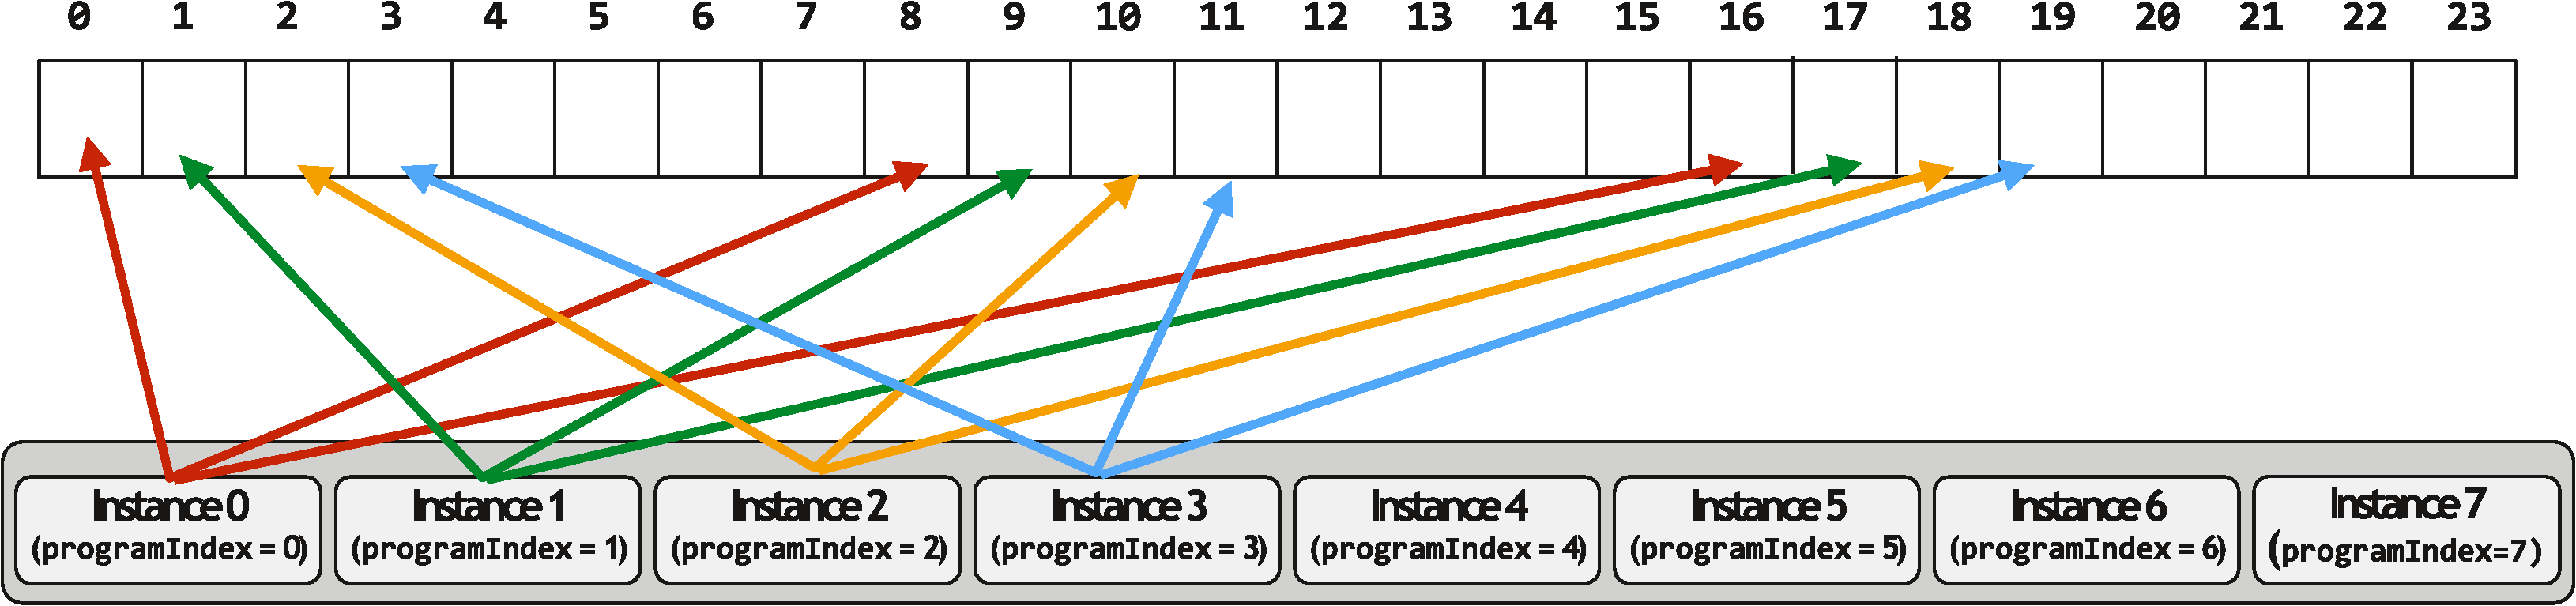
\includegraphics[width=\textwidth]{img/ispc-1.pdf}
    \begin{center}
        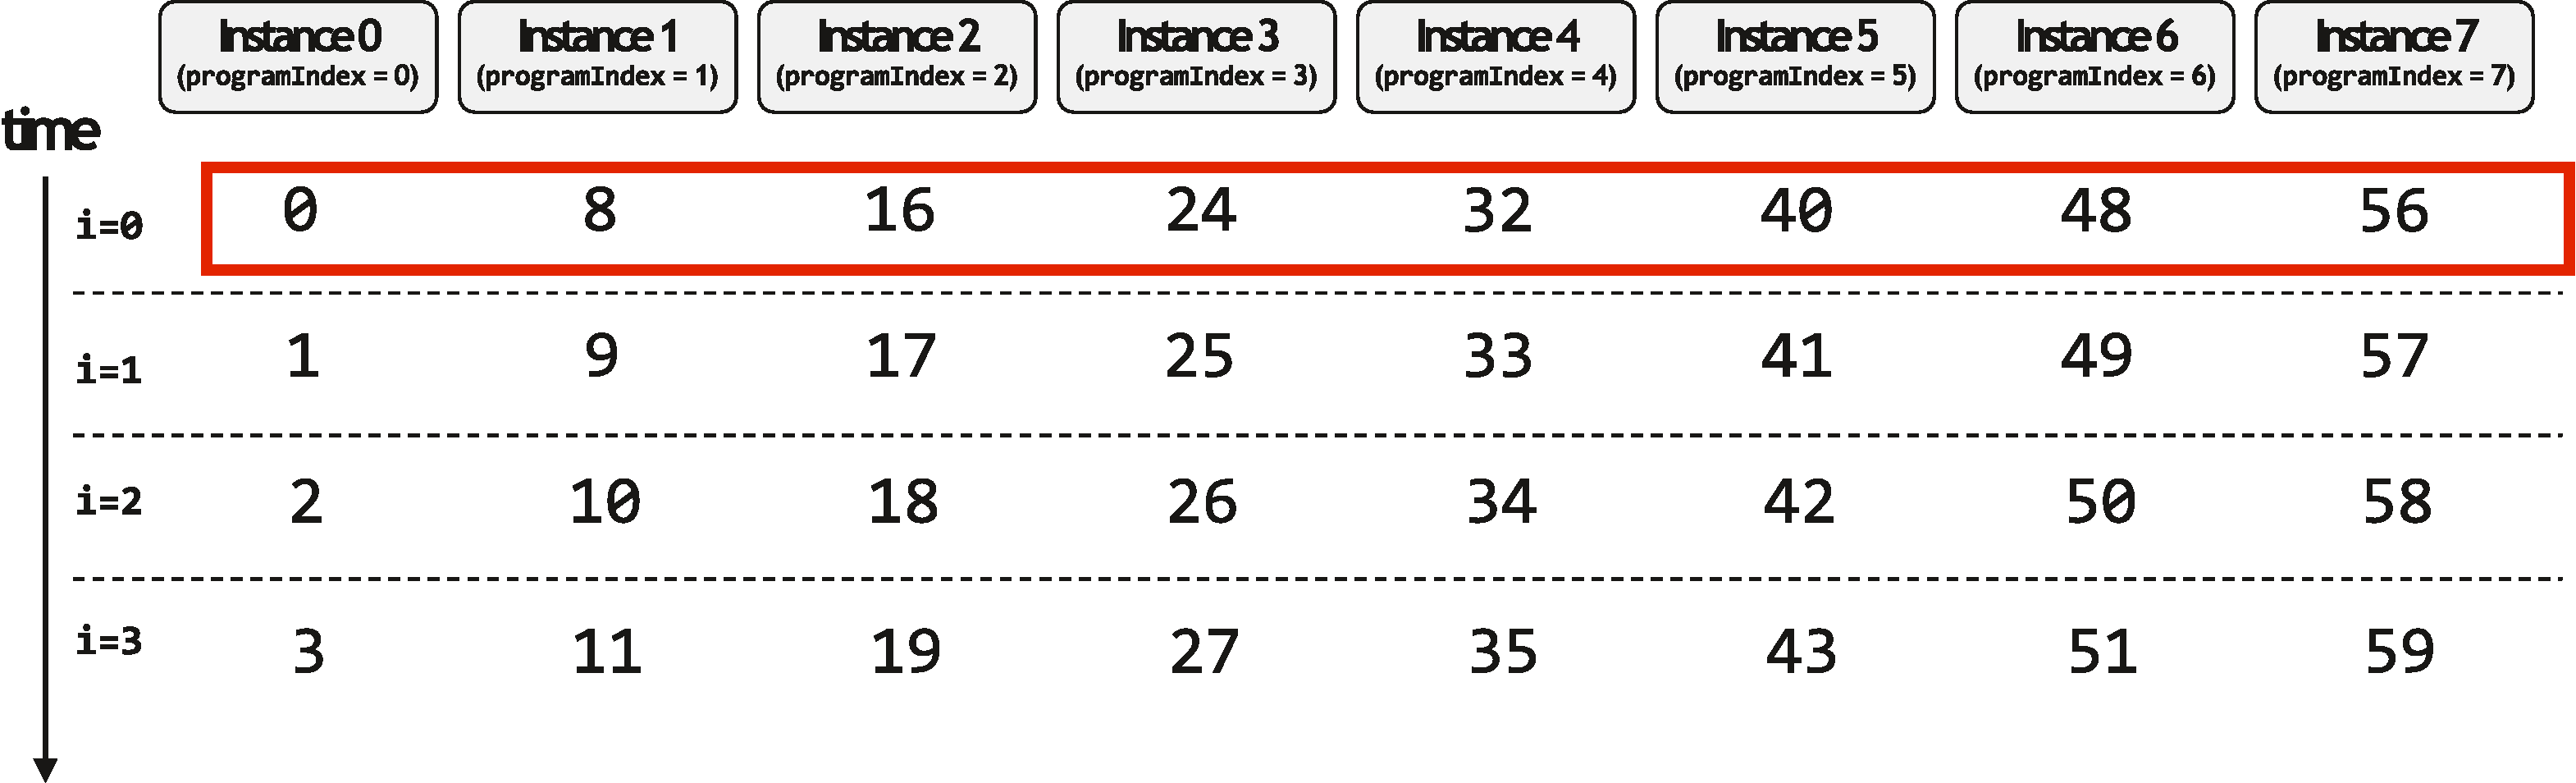
\includegraphics[width=\textwidth]{img/ispc-2.pdf}
    \end{center}
    \caption{Example of execution with 8 instances (\texttt{programCount} equal to 8). For all program instances, there are eight non-contiguous values in memory. A special instruction called \texttt{gather} is needed to implement this, but unfortunately it is a more complex and expensive SIMD instruction rather than a contiguous implementation.}
    \label{fig: ispc 8 instances, no optimized}
\end{figure}

\noindent
Figure \ref{fig: ispc 8 instances, no optimized} shows a possible execution of the ISPC function using 8 instances. The result is obtained and all is well. But there is one interesting observation. \textbf{Each ISPC instance writes each value in a non-contiguous way}. This can be done better:
\begin{lstlisting}[language=c++, mathescape]
export void ispc_sinx_v2(
    uniform int N,
    uniform int terms,
    uniform float* x,
    uniform float* result
){
    // assume N % programCount = 0
    uniform int count = N / programCount;
    int start = programIndex * count;
    for (uniform int i=0; i<count; i++) {
        int idx = start + i;
        float value = x[idx];
        float numer = x[idx] * x[idx] * x[idx];
        uniform int denom = 6; // 3!
        uniform int sign = -1;
        for (uniform int j=1; j<=terms; j++) { 
            value += sign * numer / denom
            numer *= x[idx] * x[idx];
            denom *= (j+3) * (j+4);
            sign *= -1;
        }
        result[idx] = value;
    }
}
\end{lstlisting}
\newpage
\begin{figure}[!htp]
    \centering
    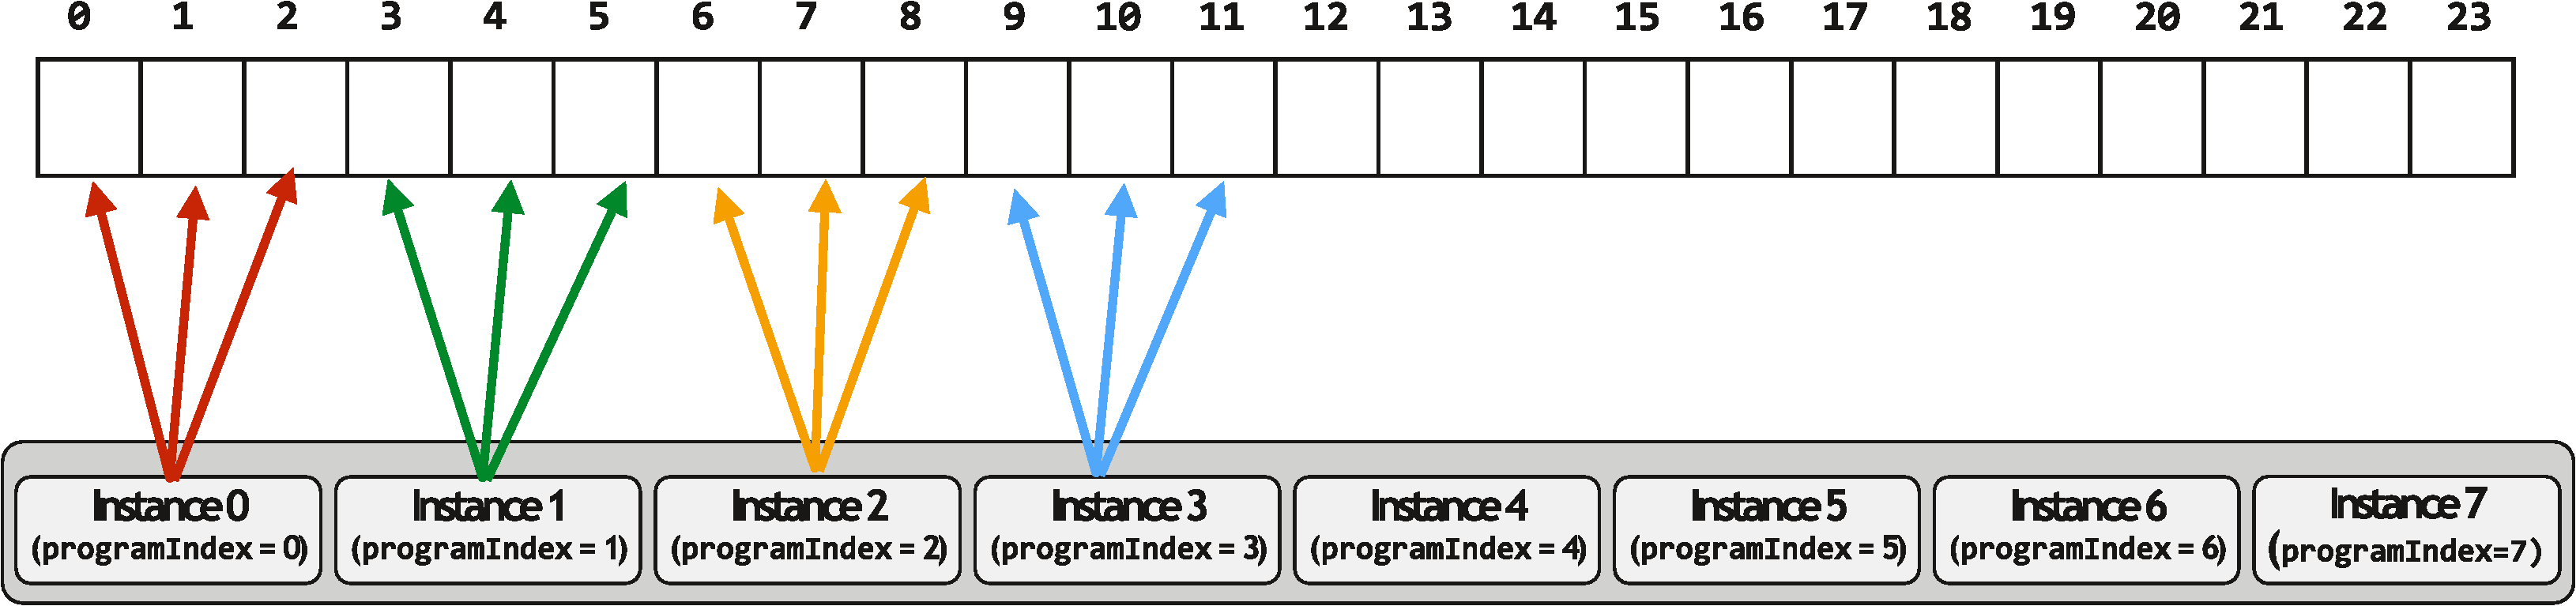
\includegraphics[width=\textwidth]{img/ispc-3.pdf}
    \begin{center}
        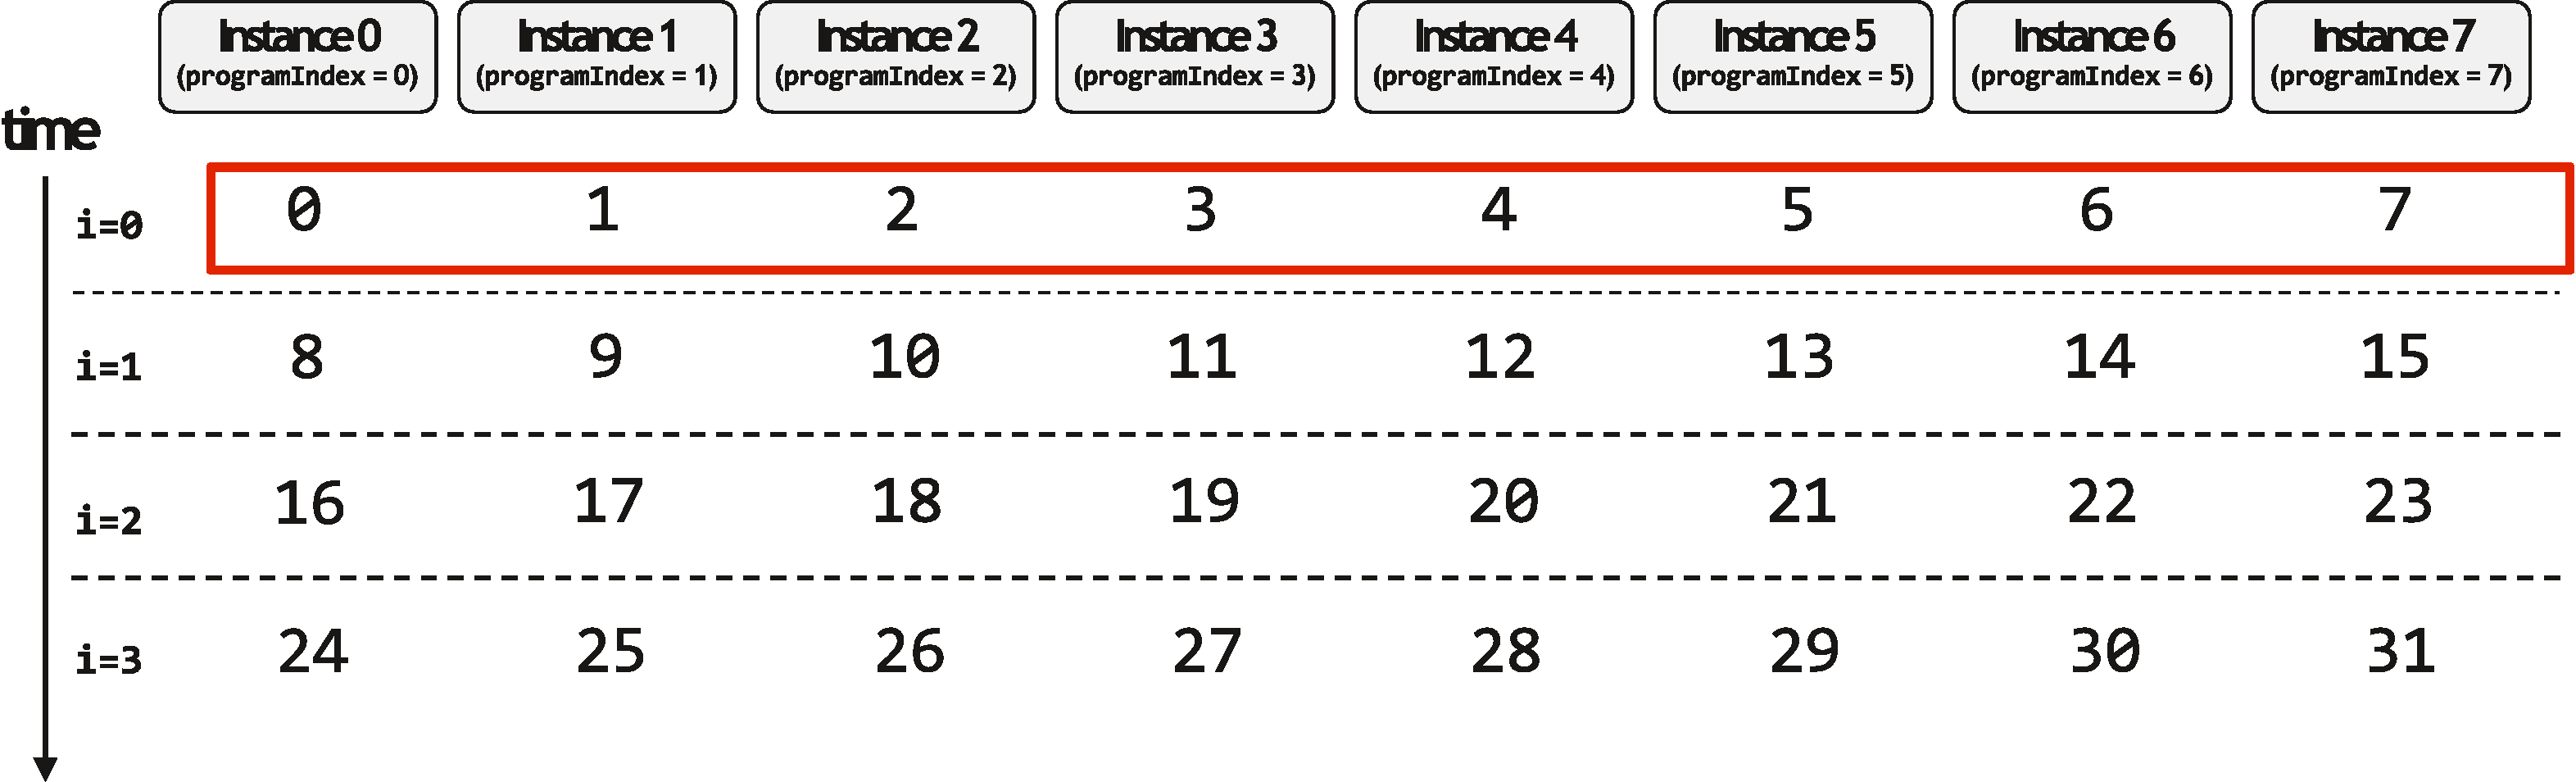
\includegraphics[width=\textwidth]{img/ispc-4.pdf}
    \end{center}
    \caption{Example of execution with 8 instances (\texttt{programCount} equal to 8). A single \dquotes{packed vector load} instruction efficiently implements this. For all program instances, since the eight values are contiguous in memory.}
\end{figure}
    \subsection{Shared Address Space Model}

We give a general introduction to memory in the chapter \ref{subsection: Accessing Memory}. In parallel computing theory, \textbf{each thread communicates with other threads using read/write operations}. These instructions operate on a special area called the \definition{Shared Address Space} (also called \definition{Shared Variables}).

\highspace
\begin{definitionbox}[: Shared Address Space]
    The \definition{Shared Address Space} view of a parallel platform supports a common data space that is accessible to all processors. Processors interact by modifying data objects stored in this shared-address-space.\cite{kumar1994introduction}
\end{definitionbox}

\highspace
Now the first and trivial question should be: a powerful tool is the possibility to allow communication between threads, but \emph{how can we guarantee that two or more threads accessing the same resource do not create well known problems, such as} \href{https://en.wikipedia.org/wiki/Race_condition#Data_race}{race condition}\emph{?}

This property, commonly called \textbf{mutual exclusion} or \textbf{atomic operation}, can be guaranteed with some techniques:
\begin{itemize}
    \item \textbf{Lock/Unlock mutex around a critical section}:
    \begin{lstlisting}[language=c++]
Lock lock_variable;

// some operations, such as spawn of threads

lock_variable.lock();
// critical section
lock_variable.unlock();\end{lstlisting}
    
    \item Some languages have first-class \textbf{support for atomicity of code blocks}:
    \begin{lstlisting}[language=c++]
atomic {
    // critical section
}\end{lstlisting}

    \item Intrinsics for \textbf{hardware-supported atomic read-modify-write operations}:
    \begin{lstlisting}[language=c++]
atomicAdd(x, 10);\end{lstlisting}
\end{itemize}
The shared address space \textbf{requires hardware support to be efficiently implemented}. The main idea is that \textbf{each processor can directly reference the contents of any memory location}. Some interesting examples that can be explored in depth are: \href{https://www.cs.rice.edu/~johnmc/comp522/lecture-notes/COMP522-2019-Lecture3-Multithreading.pdf}{SUN Niagara 2}, \href{https://ieeexplore.ieee.org/document/7477467}{Knights landing (KNL): 2nd Generation Intel Xeon Phi processor}.
    \subsection{Message passing model of communication}

In parallel computing, the \definition{message passing model} \textbf{allows} threads (or processes) to \textbf{communicate by sending and receiving messages}. This model is used to \textbf{facilitate data exchange between threads running in their own private address spaces}.

\highspace
Each thread operates within its private address space, meaning they \textbf{do not share memory directly}. When they need to communicate with a specific thread without using a \emph{shared address space model}, they use the \emph{message passing model} to send (or receive) the data.
\begin{itemize}
    \item Usually, the \textbf{sender} specifies
    \begin{itemize}
        \item the recipient;
        \item the buffer to be transmitted;
        \item an optional message identifier (a sort of tag).
    \end{itemize}
    \item Meanwhile, the \textbf{receiver} specifies:
    \begin{itemize}
        \item who the sender is;
        \item the buffer where to store data;
        \item an optional message identifier (again, a sort of tag).
    \end{itemize}
\end{itemize}
The message passing model is the \textbf{only way to exchange data between threads} because it guarantees three main advantages:
\begin{itemize}[label=\textcolor{Green3}{\faIcon{check-circle}}]
    \item \textbf{\underline{Data Isolation}}: Using message passing, \textbf{each thread maintains its address space}, reducing the risk of race conditions.

    \item \textbf{\underline{Scalability}}: Message passing \textbf{scales well with distributed systems and multi-core architectures}, making it suitable for large-scale parallel computing.
    
    \item \textbf{\underline{Flexibility}}: It \textbf{allows for explicit control over data exchange and synchronization, providing Flexibility in parallel program design}. Explicit control refers to the fact that in message passing, each communication action is explicitly defined by send and receive operations. This means we can precisely dictate which data is sent, when, and to whom it is sent. Furthermore, the synchronization is managed very well because message passing naturally incorporates synchronization. When a process sends a message, it can block until it is received, ensuring that the sender and receiver are synchronized.
\end{itemize}

\begin{flushleft}
    \textcolor{Green3}{\faIcon{question-circle} \textbf{Why message passing is preferable to the shared address space model}}
\end{flushleft}
Unlike shared memory systems that require complex hardware mechanisms to implement system-wide load and store operations, message passing systems do not need this capability. They \textbf{only need to communicate messages between nodes}. It can be considered as a great advantage for message passing models, which for this reason is very much used in the supercomputers and clusters. Finally, this model has the ability to \textbf{connect commodity hardware systems together to form a large parallel machine}. This means we can use off-the-shelf components to build powerful computing clusters.
    \subsection{Data-Parallel model}

In parallel computing, the \definition{Data-Parallel model} is characterized by \textbf{applying the same operation simultaneously across multiple data points}. This model is particularly effective for tasks involving large datasets where the same computation needs to be performed on each data element.

\highspace
This model organizes \textbf{computation as operations on sequences of elements} (e.g., perform the same function on all elements of a sequence). In programming languages, the basic data type used for this purpose is called \texttt{Sequence} (e.g., C++). Despite the name of the datatype used in the languages, the definition is that it \textbf{is an ordered collection of elements, where each element can be accessed and manipulated using various sequence operators}. The most common operators are:
\begin{itemize}
    \item \textbf{\underline{Map}}. The \texttt{map} function is a \textbf{higher-order function}\footnote{%
        A \definitionWithSpecificIndex{higher-order function}{Higher-Order function}{} is a function that can do one or both of the following:
        \begin{itemize}
            \item Take other functions as arguments (parameters).
            \item Returns a function or value as its result.
        \end{itemize}
    } that \textbf{operates on sequences}. It applies a \textbf{side-effect-free unary function}\footnote{%
        A function that takes only one argument and doesn't suffer from side effects.
    } $f : a \rightarrow b$ \textbf{to all elements of an input sequence}, producing an \textbf{output sequence of the same length}.
    \begin{examplebox}[: Python Analogy]
        For a better understanding, we provide a very simple Python code to see how a \texttt{map} function works. In Python there is a \href{https://docs.python.org/3/library/functions.html#map}{\texttt{map}} function that does exactly what we say.
        \begin{lstlisting}[language=Python]
# Define a trivial function that squares a number
def square(x):
    return x * x

# Create a sample list
numbers = [1, 2, 3, 4, 5]

# Use the map function to apply the 'square' function
# to each element in the 'numbers' list
squared_numbers = map(square, numbers)

# Convert the result to a list and print it
print(list(squared_numbers))\end{lstlisting}
        And the result is:
        \begin{lstlisting}
[1, 4, 9, 16, 25]\end{lstlisting}
    \end{examplebox}

    Now the main idea is: since the \texttt{map} is a function without side effects, we can \textbf{apply it to all elements of the sequence in any order without changing the output of the program}. This allows \textbf{reordering or parallel processing of sequence elements to \textcolor{Green4}{\textbf{optimize performance}}}.
    
    \item \textbf{\underline{Reduction}}. The reduction born from the need to make parallel operations of iterations. For example, in a \texttt{for} loop, if we need a progressive sum of an element, we should implement some kind of mechanism to manage the synchronization. Using the reduction strategies, the compiler will do this job. We suggest reading the Reduction section (\ref{paragraph: Reduction}, page \pageref{paragraph: Reduction}) in the OpenMP chapter to understand what we mean.
    
    \item Others like \textbf{\underline{scan}} and \textbf{\underline{shift}}.
\end{itemize}

    %%%%%%%%%%%%%%%%%%%%%%%%%%%%%%%%%%%%%%%%%%%%%%%%%
    % Parallel Programming Models and POSIX Threads %
    %%%%%%%%%%%%%%%%%%%%%%%%%%%%%%%%%%%%%%%%%%%%%%%%%
    \section{Parallel Programming Models and pthreads}

\subsection{How to create parallel algorithms and programs}

Although \emph{parallel algorithms} and \emph{parallel programs} are in the same father set, the parallel computing topic, these two arguments are a little different.

\begin{definitionbox}[: Parallel Algorithms]
    A \definitionWithSpecificIndex{parallel algorithm}{Parallel Algorithm}{}, as opposed to a traditional serial algorithm, is an \textbf{algorithm which can do multiple operations in a given time}.
\end{definitionbox}

\begin{definitionbox}[: Parallel Programs]
    A \definitionWithSpecificIndex{parallel program}{Parallel Program}{} is a \textbf{program that uses multiple CPU cores}, with \textbf{each core performing a task independently}.
\end{definitionbox}

\noindent
However, designing \emph{parallel algorithms} is not an easy task because there is no heuristic for designing \emph{parallel algorithms}. There are some rules that help in the design. The same reasoning applies to \emph{parallel programs}, because they depend on the chosen language and architecture.

\highspace
Furthermore, there is no single correct solution, but several possible parallel solutions. A \textbf{good first approach is to start with machine-independent issues} (concurrency) and \textbf{delay target-specific issues as much as possible}.

\begin{table}[!htp]
    \centering
    \begin{tabular}{@{} p{16em} p{16em} @{}}
        \toprule
        Design a parallel algorithm & Design a parallel program \\
        \midrule
        Understand the problem to be solved & Analyze the target architecture(s) \\
        \cmidrule{1-2}
        Analyze data dependencies & Choose the best parallel programming model and language \\
        \cmidrule{1-2}
        Partition the solution & Analyze the communications (cost, latency, bandwidth, visibility, synchronization, etc.) \\
        \bottomrule
    \end{tabular}
    \caption{Design parallel algorithms and parallel programs.}
\end{table}

\noindent
The \definition{PCAM (Partitioning, Communication, Agglomeration, Mapping)} methodology described by \href{https://www.mcs.anl.gov/~itf/dbpp/text/node15.html}{Argonne National Laboratory} is intended to promote an exploratory \textbf{approach to design in which machine independent issues}, such as \emph{concurrency}, are \textbf{considered early} and \textbf{machine specific aspects of design are deferred until late in the design process}. In other words, we immediately consider the machine-independent issues (e.g., concurrency) at the beginning of the design approach, and all machine-specific aspects are postponed to an advanced stage of the design process.

\newpage
\noindent
This methodology structures the design process into \textbf{four distinct stages}: 
\begin{enumerate}
    \item \textbf{\underline{Partitioning}}. The \textbf{computation} that is to be performed and the \textbf{data} operated on by this computation are \textbf{decomposed into small tasks}. Practical issues such as the number of processors in the target computer are ignored, and attention is focused on recognizing opportunities for parallel execution.

    \item \textbf{\underline{Communication}}. The communication required to \textbf{coordinate task execution} is determined, and appropriate \textbf{communication structures and algorithms are defined}.

    \item \textbf{\underline{Agglomeration}}. The task and \textbf{communication structures} defined in the first two stages of a design are \textbf{evaluated with respect to performance requirements and implementation costs}. If necessary, tasks are combined into larger tasks to improve performance or to reduce development costs.     

    \item \textbf{\underline{Mapping}}. \textbf{Each task is assigned to a processor} in a manner that attempts to satisfy the competing goals of \textbf{maximizing processor utilization} and \textbf{minimizing communication costs}. Mapping can be specified statically or determined at runtime by load-balancing algorithms.
\end{enumerate}
In the \textbf{first two stages}, we focus on \example{concurrency} and \example{scalability} and seek to \textbf{discover algorithms with these qualities}. In the \textbf{third and fourth stages}, attention shifts to \example{locality} and \example{other performance-related issues}.
\begin{figure}[!htp]
    \centering
    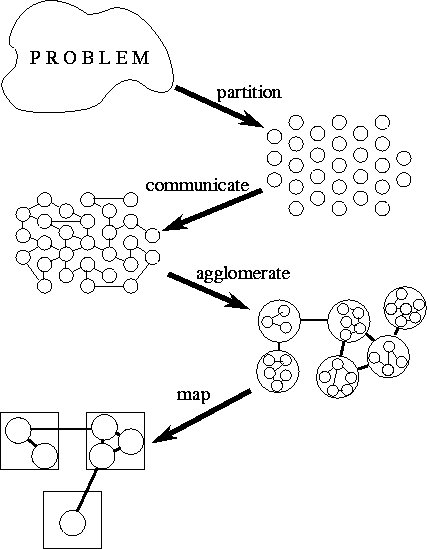
\includegraphics[width=.5\textwidth]{img/pcam-1.png}
    \caption{PCAM design methodology for parallel programs. Starting with a problem specification, develop a partition, determine communication requirements, agglomerate tasks, and finally map tasks to processors.}
\end{figure}
    \subsection{Analyze parallel algorithms}

Whether we want to analyze our parallel algorithm created with the PCAM model or evaluate a general parallel algorithm, we need some metrics.

\highspace
The classical \textbf{metrics} needed to evaluate a parallel algorithm are:
\begin{itemize}
    \item \textbf{Time complexity}: quantifies the amount of \textbf{time required to produce a solution}.
    \item \textbf{Resource complexity}: quantifies how many \textbf{resources are needed to produce the solution in that time}.
\end{itemize}
In general, to analyze a \textbf{parallel algorithm}, we can consider its \textbf{structure as a directed acyclic graph (DAG)}\footnote{A \definition{Directed Acyclic Graph (DAG)} is a directed graph, i.e. with oriented edges, without cycles.}, where the nodes are the task and the edges are the data dependencies.

\highspace
\begin{flushleft}
    \textcolor{Red2}{\faIcon{book} \textbf{Parallel Algorithm Terminology and Metrics}}
\end{flushleft}
\begin{itemize}
    \item \definitionWithSpecificIndex{Concurrent tasks}{Concurrent tasks in parallel algorithms}{}, each task is executed \emph{\textbf{independently}}.
    
    \item \definitionWithSpecificIndex{Parallel tasks}{Parallel tasks in parallel algorithms}{}, each task is executed at the \emph{\textbf{same time}} (because multiple computing resources are available).
    
    \item \definitionWithSpecificIndex{Work $W$}{Work metric for parallel algorithms}{} is the \emph{\textbf{number of operations executed}}. It may be higher than the sequential version of the algorithm due to communication overhead, etc.
    
    \item \definitionWithSpecificIndex{Span $S$}{Span metric for parallel algorithms}{} is the \emph{\textbf{longest chain of dependencies}} (i.e., the critical path) that determines the \emph{\textbf{minimum time required to execute the algorithm}}. This is a \emph{lower bound} on the running time, regardless of the number of processors. The range indicates the ability of an algorithm to get better performance on more processors.
    \begin{flushleft}
        \textcolor{Green3}{\faIcon{question-circle} \textbf{How do we calculate the Span metric?}}
    \end{flushleft}
    \begin{enumerate}
        \item As we just said, we \textbf{represent a parallel algorithm as a DAG} graph, where nodes represent tasks and edges represent dependencies between tasks;
        \item We \textbf{assign weights to each node} that represent the \textbf{time required to perform the corresponding task};
        \item We try to \textbf{find the Critical Path}. In other words, we determine the path from the start node to the end node that has the \emph{maximum cumulative weight};
        \item Finally, the \textbf{sum} of the \textbf{weights of the nodes on the critical path} gives us the span value!
    \end{enumerate}

    \newpage
    \item \definitionWithSpecificIndex{Parallelism $P$}{Parallelism metrico for parallel algorithms}{} is the \emph{\textbf{measure of efficiency in the use of resources}}. Trivially, it is the number of operations performed divided by the longest chain of dependencies:
    \begin{equation}
        P = \dfrac{W}{S}
    \end{equation}
    It indicates \textbf{how many processors can be effectively used by the computation}. If the work is equal to the span, the parallelism is 1 and the computation is sequential. Ideally, but not necessarily, we win with polylogarithmic span, because if the work is $O(n \log n)$ and the span is $O(\log^{2} n)$, then the parallelism is $O\left(\frac{n}{\log n}\right)$, which is actually quite high (and unlikely to be a bottleneck on most machines in the next 25 years).\cite{introductionToParallelAlgorithmsUMD}

    This measure is \emph{one of the most important}. It indicates the \textbf{number of processors that are not idle}. It is obvious that a \textbf{good parallel algorithm is designed to have the lowest possible work} (less operation, then less resource usage, then less cost, and so on) \textbf{and the highest possible parallelism} (achievable by reducing the span, and this should be trivial, since the metric $P$ is given by work divided by the span, so reducing the denominator, you can get a higher value).

    As in all things, there is a \textbf{trade-off} between the lowest possible \dquotes{work} and the highest possible \dquotes{parallelism}. Reducing the work too much could eliminate the possibility of parallelizing our algorithm, and on the other hand, reducing the span too aggressively could cause communication/synchronization overhead.
\end{itemize}

\begin{figure}[!htp]
    \centering
    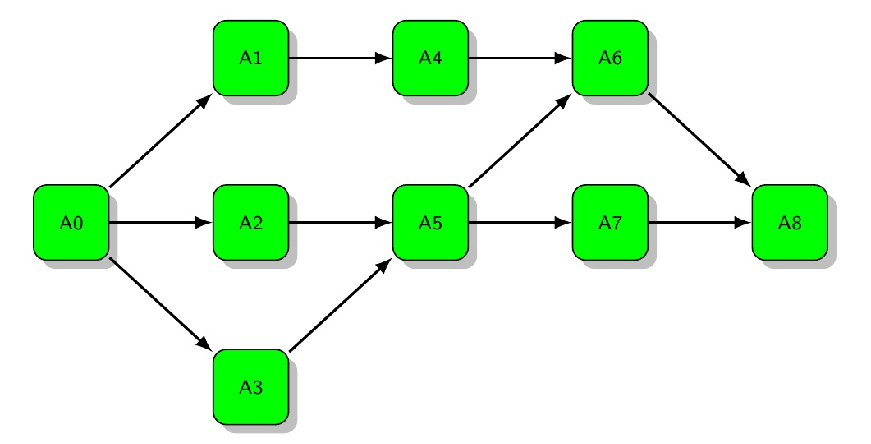
\includegraphics[width=.7\textwidth]{img/dag-1.pdf}
    \caption{Example of DAG implementation with work equal to 9, span equal to 5, and parallelism equal to 1.8 ($9 \div 5$). The span calculus is not well known, has been calculated \emph{a priori}.}
\end{figure}

\noindent
Finally, we use a mathematical annotation and not only a graphical (DAG) annotation. The \definition{Composition Rules} help determine how to combine smaller parallel tasks into a larger algorithm, while analyzing the Work and Span of the combined algorithm:
\begin{itemize}
    \item \textbf{Single operation}. An operation takes 1 unit of work and 1 unit of span time.
    \begin{equation*}
        W\left(op\right) = 1 \hspace{2em} S\left(op\right) = 1
    \end{equation*}

    \newpage

    \item \textbf{Sequential Composition}.
    \begin{itemize}
        \item The total work of executing $e_{1}$ and $e_{2}$ \textbf{sequentially} is the sum of their individual work.
        \begin{equation*}
            W\left(e_{1}, e_{2}\right) = W\left(e_{1}\right) + W\left(e_{2}\right)
        \end{equation*}

        \item The total span of executing $e_{1}$ and $e_{2}$ \textbf{sequentially} is the sum of their individual spans.
        \begin{equation*}
            S\left(e_{1}, e_{2}\right) = S\left(e_{1}\right) + S\left(e_{2}\right)
        \end{equation*}
    \end{itemize}
    
    \item \textbf{Parallel Composition}.
    \begin{itemize}
        \item The total work of executing $e_{1}$ and $e_{2}$ in \textbf{parallel} is still the sum of their individual works.
        \begin{equation*}
            W\left(e_{1} || e_{2}\right) = W\left(e_{1}\right) + W\left(e_{2}\right)
        \end{equation*}

        \item The total span of executing $e_{1}$ and $e_{2}$ in \textbf{parallel} is the \emph{\textbf{maximum of their individual spans}}, since they can be executed simultaneously.
        \begin{equation*}
            S\left(e_{1} || e_{2}\right) = \max\left(W\left(e_{1}\right), W\left(e_{2}\right)\right)
        \end{equation*}
    \end{itemize}
\end{itemize}
    \subsection{Technologies}

Some famous architecture to work with parallel programming:
\begin{itemize}
    \item \textbf{\underline{Verilog/VHDL}} are \emph{hardware description languages}. The target architectures are \emph{ASIC and FPGA}. The \textbf{parallelism} and the \textbf{communication} are \textbf{explicit}.
    \begin{flushleft}
        \textcolor{Green3}{\faIcon{check} \textbf{Pros}}
    \end{flushleft}
    \begin{itemize}
        \item Complete control on computation and memory
        \item No overhead introduced in the computation
        \item Provides access to potentially large computational power
    \end{itemize}
    \begin{flushleft}
        \textcolor{Red2}{\faIcon{exclamation-triangle} \textbf{Cons}}
    \end{flushleft}
    \begin{itemize}
        \item Requires specific hardware (e.g., ASIC or FPGA) to implement functionality
        \item Difficult to learn: completely different programming language and programming paradigm
        \item Depends on the chosen target architecture
    \end{itemize}

    \item \textbf{\underline{MPI}} is a \emph{library}. The target architectures are \emph{Multi CPUs}. The \textbf{parallelism} is \textbf{implicit} and the \textbf{communication} is \textbf{explicit}.
    \begin{flushleft}
        \textcolor{Green3}{\faIcon{check} \textbf{Pros}}
    \end{flushleft}
    \begin{itemize}
        \item Can be adopted on different types of architecture
        \item Scalable solutions
        \item Synchronization and data communication are explicitly managed
    \end{itemize}
    \begin{flushleft}
        \textcolor{Red2}{\faIcon{exclamation-triangle} \textbf{Cons}}
    \end{flushleft}
    \begin{itemize}
        \item Communication can introduce significant overhead
        \item Programming paradigm more difficult than shared memory-based ones
        \item Standard does not reflect immediately advances in architecture characteristics
    \end{itemize}

    \item \textbf{\underline{PThread}} is a \emph{library}. The target architectures are \emph{Multi-core CPUs}. The \textbf{parallelism} is \textbf{explicit} and the \textbf{communication} is \textbf{implicit}.
    \begin{flushleft}
        \textcolor{Green3}{\faIcon{check} \textbf{Pros}}
    \end{flushleft}
    \begin{itemize}
        \item Can be adopted on different types of architecture
        \item Explicit parallelism and full control over application
    \end{itemize}
    \begin{flushleft}
        \textcolor{Red2}{\faIcon{exclamation-triangle} \textbf{Cons}}
    \end{flushleft}
    \begin{itemize}
        \item Task management overhead can be significant
        \item Not easily scalable solutions
        \item Low level API
    \end{itemize}

    \item \textbf{\underline{OpenMP}} is a \emph{C/Fortran extensions}. The target architectures are \emph{Multi-core CPUs}. The \textbf{parallelism} is \textbf{explicit} and the \textbf{communication} is \textbf{implicit}.
    \begin{flushleft}
        \textcolor{Green3}{\faIcon{check} \textbf{Pros}}
    \end{flushleft}
    \begin{itemize}
        \item Easy to learn
        \item Scalable solution
        \item Parallel applications can also be executed sequentially
    \end{itemize}
    \begin{flushleft}
        \textcolor{Red2}{\faIcon{exclamation-triangle} \textbf{Cons}}
    \end{flushleft}
    \begin{itemize}
        \item Mainly focused on shared memory homogeneous systems
        \item Requires small interaction between tasks
    \end{itemize}

    \item \textbf{\underline{CUDA}} is a \emph{C extensions}. The target architectures are \emph{CPU plus GPU(s)}. The \textbf{parallelism} is \textbf{implicit/explicit} and the \textbf{communication} is \textbf{implicit/explicit}.
    \begin{flushleft}
        \textcolor{Green3}{\faIcon{check} \textbf{Pros}}
    \end{flushleft}
    \begin{itemize}
        \item Provides access to the computational power of GPUs
        \item Writing a CUDA kernel is quite easy
        \item Already optimized libraries
    \end{itemize}
    \begin{flushleft}
        \textcolor{Red2}{\faIcon{exclamation-triangle} \textbf{Cons}}
    \end{flushleft}
    \begin{itemize}
        \item Targets only NVIDIA GPUs
        \item Difficult to extract massive parallelism from application
        \item Difficult to optimize CUDA kernel
    \end{itemize}

    \item \textbf{\underline{OpenCL}} is a \emph{C/C++ extensions and API}. The target architectures are \emph{heterogeneous architecture}. The \textbf{parallelism} is \textbf{implicit/explicit} and the \textbf{communication} is \textbf{implicit/explicit}.
    \begin{flushleft}
        \textcolor{Green3}{\faIcon{check} \textbf{Pros}}
    \end{flushleft}
    \begin{itemize}
        \item Target-independent standard
        \item Hides architecture details
        \item Same programming infrastructure for every heterogeneous architecture: CPU + GPU (and FPGA)
    \end{itemize}
    \begin{flushleft}
        \textcolor{Red2}{\faIcon{exclamation-triangle} \textbf{Cons}}
    \end{flushleft}
    \begin{itemize}
        \item Difficult programming paradigm for its heterogeneity
        \item Hiding of architecture details makes difficult to obtain best performances
        \item Gradually abandoned
    \end{itemize}

    \item \textbf{\underline{Apache Spark}} is an \emph{API}. The target architectures are \emph{multi CPUs}. The \textbf{parallelism} is \textbf{implicit} and the \textbf{communication} is \textbf{implicit}.
    \begin{flushleft}
        \textcolor{Green3}{\faIcon{check} \textbf{Pros}}
    \end{flushleft}
    \begin{itemize}
        \item API for different languages
        \item Explicit parallelization and communication are not required
        \item Preinstalled on cloud provide VMs
    \end{itemize}
    \begin{flushleft}
        \textcolor{Red2}{\faIcon{exclamation-triangle} \textbf{Cons}}
    \end{flushleft}
    \begin{itemize}
        \item Suitable only for big data applications
        \item Does not (yet) fully support GPUs
    \end{itemize}
\end{itemize}
Regardless of these technologies, it is quite common to mix some of them:
\begin{itemize}
    \item \textbf{OpenMP + CUDA}: allows to exploit multi-core CPU and GPU. CUDA is used to parallelize GPU code and OpenMP is used to parallelize CPU code.
    
    \item \textbf{MPI + OpenMP}: the most common scenario are:
    \begin{enumerate}
        \item MPI used to express coarser parallelism (multi CPU) and OpenMP used to express finer parallelism (multi core).
        \item MPI used to implement communication and OpenMP used to parallelize computation.
    \end{enumerate}

    \item \textbf{OpenCL + Verilog or VHDL}: in principle, hardware kernels (implemented for example on FPGA) can be used as accelerators; OpenMP used to describe parallelism among different processing elements; Verilog/VHDL used to describe hardware kernel. An example of target: Intel Xeon Scalable.
\end{itemize}
    \subsection{Threads}

\subsubsection{Flynn's taxonomy}

\definition{Flynn's taxonomy} is a \textbf{classification of computer architectures}, proposed by Michael J. Flynn. The classification system has been used as a tool in the design of modern processors and their functionalities. Since the rise of multiprocessing central processing units (CPUs), a multiprogramming context has evolved as an extension of the classification system.

\highspace
The four initial classifications defined by Flynn are based upon the number of concurrent instruction (or control) streams and data streams available in the architecture:
\begin{itemize}
    \item \textbf{Single Instruction stream, Single Data stream (SISD)}
    \item \textbf{Single Instruction stream, Multiple Data streams (SIMD)}
    \item \textbf{Multiple Instruction stream, Single Data stream (MISD)}
    \item \textbf{Multiple Instruction stream, Multiple Data stream (MISD)}
\end{itemize}
It is important to quote it because it is the basis for the development of many advanced technologies.

\longline

\subsubsection{Definition}

A UNIX process can be created by the operating system and contains information about program resources and program execution status.

\begin{definitionbox}[: Thread]
    A \definitionWithSpecificIndex{thread}{Thread}{} is an \textbf{independent stream of instructions within a process}. Threads can be scheduled by the operating system, and each thread can run concurrently with other threads. A thread also has local resources and can access the shared process resources.
\end{definitionbox}

\noindent
In other words, a thread can be thought of as any \textbf{procedure that runs independently of its main program}. We can create each thread dynamically during execution. A good point is that a multi-threaded program is lighter than a multi-process program.

\newpage
\noindent
When a thread exists within a process, it shares most of the process resources, for example:
\begin{itemize}
    \item Changes made by one thread to shared system resources (such as closing a file) will be seen by all other threads.
    \item Two pointers having the same value point to the same data.
    \item \textbf{Implicit communication} by reading and writing shared variables.
    \item \textbf{Reading and writing to the same memory locations requires explicit synchronization by the programmer}. If this rule is not followed, the code may suffer from a data race or race condition \footnote{In parallel computing, a \definition{Data Race} or \definition{Race Condition}\label{def: race condition} is a software problem that occurs when two threads (or processes) access the same variables, and at least one does a write. They can finish in a different order than expected.} problem.
\end{itemize}
The most common models for threaded programs are the manager / worker model\footnote{The manager/worker pattern is described as follows. The idea is that the work that needs to be done can be divided by a \dquotes{manager} into separate pieces and the pieces can be assigned to individual \dquotes{worker} processes. Thus the manager executes a different algorithm from that of the workers, but all of the workers execute the same algorithm. Most implementations of MPI allow MPI processes to be running different programs (executable files), but it is often convenient (and in some cases required) to combine the manager and worker code into a single program.} and pipeline.

\highspace
This chapter introduces the POSIX threads model.
\begin{definitionbox}[: pthreads]
    \definition{POSIX Threads}, commonly known as \textbf{pthreads}, is an \textbf{execution model} that exists independently from a programming language, as well as a parallel execution model. It \textbf{allows a program to control multiple different flows of work that overlap in time}. Each flow of work is referred to as a thread, and creation and control over these flows is achieved by making calls to the POSIX Threads API.
\end{definitionbox}

\noindent
POSIX threads and OpenMP are two \textbf{implementations of a shared memory parallel programming model using threads}. The \textbf{programmer is responsible for handling parallelism and synchronization}, usually through a library of subroutines or a set of compiler directives. Typically, hardware vendors have implemented their own proprietary versions of threads, but in this course we will look at POSIX threads (pthreads) and OpenMP.

\newpage

\subsubsection{pthreads API}

In 1995, the IEEE POSIX 1003.1c standard specified the API for explicitly managing threads. An \textbf{API is a set of C language programming types and procedure calls}.
\begin{itemize}
    \item \textbf{Header file} to include in the main file: \texttt{pthread.h}.
    \item To \textbf{compile} and use it, it is necessary to add the \textbf{flag} \texttt{-pthread} to the gcc (or g++) options.
\end{itemize}
The API are divided by what we want to do. In general, there are two sets: thread management and thread synchronization.
\begin{itemize}
    \item Thread Management
    \begin{itemize}
        \item Creation (page \pageref{paragraph: Creation})
        \item Termination (page \pageref{paragraph: Termination})
        \item Joining (page \pageref{paragraph: Joining})
        \item Detaching (page \pageref{paragraph: Detaching})
        \item Joining through Barriers (page \pageref{paragraph: Joining through Barriers})
    \end{itemize}
    \item Thread Synchronization
    \begin{itemize}
        \item Mutexes (page \pageref{paragraph: Mutexes})
        \item Condition variables (page \pageref{paragraph: Condition variables})
    \end{itemize}
\end{itemize}

\longline

\paragraph{Creation}\label{paragraph: Creation}

Once threads are created, they are peers, and \textbf{may create other threads}. There is \textbf{no implied hierarchy or dependency between threads}. The \textbf{maximum number of threads depends on the implementation}.
\marginpar{
    \href{https://man7.org/linux/man-pages/man3/pthread_create.3.html} {Doc. \faIcon{book}}
}
\begin{pthreadbox}[: \texttt{pthread\_create}]
    \begin{lstlisting}[language=c++]
int pthread_create(
    pthread_t * thread,
    const pthread_attr_t * attr,
    void * (* start_routine) (void *),
    void * arg
)\end{lstlisting}
\end{pthreadbox}

\noindent
\begin{itemize}
    \item \textbf{Return value}: on success, \texttt{pthread\_create()} returns 0; on error, it returns an error number, and the contents of \texttt{*thread} are undefined.
    \item \textbf{Arguments}:
    \begin{itemize}
        \item \texttt{thread}: identifier for the new thread returned by the subroutine.
        \item \texttt{attr}: used to set thread attributes, such as joinable, detached, scheduling and stack size.
        \item \texttt{start\_routine}: the C routine that the thread will execute once it is created.
        \item \texttt{arg}: argument passed to \texttt{start\_routine}. It must be passed by address as a pointer cast of type void.
    \end{itemize}
\end{itemize}

\longline

\paragraph{Termination}\label{paragraph: Termination}

The thread returns from its startup routine when its \dquotes{life} ends. The thread makes a call to the \texttt{pthread\_exit} subroutine.
\marginpar{
    \href{https://man7.org/linux/man-pages/man3/pthread_exit.3.html} {Doc. \faIcon{book}}
}
\begin{pthreadbox}[: \texttt{pthread\_exit}]
    \begin{lstlisting}[language=c++]
void pthread_exit(void *retval)\end{lstlisting}
\end{pthreadbox}
\begin{itemize}
    \item \textbf{Return value}: this function does not return to the caller.
    \item \textbf{Arguments}:
    \begin{itemize}
        \item \texttt{retval}: function terminates the calling thread and returns a value via \texttt{retval}.
    \end{itemize}
\end{itemize}

\highspace
The thread is canceled by another thread via the \texttt{pthread\_cancel} routine.
\marginpar{
    \href{https://man7.org/linux/man-pages/man3/pthread_cancel.3.html} {Doc. \faIcon{book}}
}
\begin{pthreadbox}[: \texttt{pthread\_cancel}]
    \begin{lstlisting}[language=c++]
int pthread_cancel(pthread_t thread)\end{lstlisting}
\end{pthreadbox}
\begin{itemize}
    \item \textbf{Return value}: on success, \texttt{pthread\_cancel()} returns 0; on error, it returns a nonzero error number.
    \item \textbf{Arguments}:
    \begin{itemize}
        \item \texttt{thread}: the \texttt{pthread\_cancel()} function sends a cancellation request to the thread \texttt{thread}.
    \end{itemize}
\end{itemize}

\newpage

\paragraph{Joining}\label{paragraph: Joining}

The join function \textbf{blocks the calling thread until the specified thread exits}.
\marginpar{
    \href{https://man7.org/linux/man-pages/man3/pthread_join.3.html} {Doc. \faIcon{book}}
}
\begin{pthreadbox}[: \texttt{pthread\_join}]
    \begin{lstlisting}[language=c++]
int pthread_join(pthread_t thread, void **retval)\end{lstlisting}
\end{pthreadbox}
\begin{itemize}
    \item \textbf{Return value}: on success, \texttt{pthread\_join()} returns 0; on error, it returns an error number.
    \item \textbf{Arguments}:
    \begin{itemize}
        \item \texttt{thread}: the \texttt{pthread\_join()} function waits for the thread specified by \texttt{thread} to terminate. If that thread has already terminated, then \texttt{pthread\_join()} returns immediately. The thread specified by \texttt{thread} must be joinable.
        
        If multiple threads simultaneously try to join with the same thread, the results are undefined.  If the thread calling \texttt{pthread\_join()} is canceled, then the target thread will remain joinable (i.e., it will not be detached).
        
        \item \texttt{retval}: if \texttt{retval} is not \texttt{NULL}, then \texttt{pthread\_join()} copies the exit status of the target thread (i.e., the value that the target thread supplied to \texttt{pthread\_exit()}) into the location pointed to by \texttt{retval}. If the target thread was canceled, then \texttt{PTHREAD\_CANCELED} is placed in the location pointed to by \texttt{retval}.
    \end{itemize}
\end{itemize}

\newpage

\paragraph{Detaching}\label{paragraph: Detaching}

The detach function \textbf{marks a thread as detached}. When a thread is detached, its \textbf{resources are automatically released back to the system when the thread terminates}, without the need for another thread to join with it.
\begin{flushleft}
    \textcolor{Green3}{\faIcon{question-circle} \textbf{Why would I need to detach a thread and not join it?}}
\end{flushleft}
Good question. The answer depends on what we have to do.
\begin{itemize}
    \item \textbf{Fire and forget tasks}. When we start a thread to perform a task that doesn't require further interaction or result processing, releasing it ensures that the resources are automatically cleaned up when the task is complete.

    \item \textbf{Resource management}. Detaching avoids the need for another thread to call \texttt{pthread\_join()}, which can save system resources and reduce the complexity of our code. It's especially useful in a highly concurrent application with many short-lived threads.
    
    \item \textbf{Avoid deadlocks}. When we have potential circular dependencies or complex synchronization between threads, detaching threads can help avoid deadlocks by eliminating the need for one thread to wait on another.
    
    \item \textbf{Long-running background tasks}. For tasks that should run independently in the background and not block the main program flow, detaching makes sense. We make sure they clean up after themselves without having to explicitly manage their lifecycle.
\end{itemize}
\marginpar{
    \href{https://man7.org/linux/man-pages/man3/pthread_detach.3.html} {Doc. \faIcon{book}}
}
\begin{pthreadbox}[: \texttt{pthread\_detach}]
    \begin{lstlisting}[language=c++]
int pthread_detach(pthread_t thread)\end{lstlisting}
\end{pthreadbox}
\begin{itemize}
    \item \textbf{Return value}: on success, \texttt{pthread\_detach()} returns 0; on error, it returns an error number.
    \item \textbf{Arguments}:
    \begin{itemize}
        \item \texttt{thread}: the \texttt{pthread\_detach()} function marks the thread identified by \texttt{thread} as detached.  When a detached thread terminates, its resources are automatically released back to the system without the need for another thread to join with the terminated thread.
 
        Attempting to detach an already detached thread results in unspecified behavior.
    \end{itemize}
\end{itemize}

\newpage

\paragraph{Joining through Barriers}\label{paragraph: Joining through Barriers}

The \emph{barrier init} function \textbf{initializes a barrier object}, and the \emph{barrier wait} function \textbf{blocks a thread until the specified number of threads have called it}. A \definitionWithSpecificIndex{barrier object}{Barrier Object}{} is, in parallel computing, a synchronization tool that ensures that multiple threads reach a certain point of execution before any of them continue. It's like a \textbf{checkpoint that everyone must reach before continuing}, ensuring coordinated progress in a parallel algorithm.\footnote{For example, imagine multiple threads working on different parts of a matrix. A barrier can ensure that all threads finish their part of the computation before moving on to the next phase, such as combining results or performing subsequent operations.}
\marginpar{
    \href{https://linux.die.net/man/3/pthread_barrier_init} {Doc. \faIcon{book}}
}
\begin{pthreadbox}[: \texttt{pthread\_barrier\_init}]
    \begin{lstlisting}[language=c++]
int pthread_barrier_init(
    pthread_barrier_t * barrier,
    pthread_barrierattr_t * attr,
    unsigned int count
)\end{lstlisting}
\end{pthreadbox}
\begin{pthreadbox}[: \texttt{pthread\_barrier\_wait}]
    \begin{lstlisting}[language=c++]
int pthread_barrier_wait(pthread_barrier_t * barrier)\end{lstlisting}
\end{pthreadbox}
\begin{itemize}
    \item \textbf{Return value}: on success, function return 0; on error, they return an error number.
    \item \textbf{Arguments}: the main and most important argument is \texttt{count}, which specifies the \textbf{number of threads to wait} for.
\end{itemize}

\newpage

\paragraph{Mutexes}\label{paragraph: Mutexes}

Mutex variables are the basic \textbf{method of protecting shared data when multiple writes occur}. Only \textbf{one thread can lock a mutex variable at a time}. If multiple threads attempt to lock a mutex, only one thread will succeed. \textbf{Threads that fail to acquire the mutex are blocked}. There is also the \texttt{trylock} function, which returns immediately if the mutex is currently locked (by any thread, including the current thread). Note that a \textbf{lock function has the potential to create a deadlock situation}.

\highspace
There are also \textbf{three types of mutex} that can be set using the \texttt{settype} function:
\begin{itemize}
    \item \definition{Normal Mutex (\texttt{PTHREAD\_MUTEX\_NORMAL})}. A \textbf{normal mutex does not check for errors such as deadlock}. If a thread tries to lock a mutex it already owns, the thread will deadlock.
    \item \definition{Error Check Mutex (\texttt{PTHREAD\_MUTEX\_ERRORCHECK})}. Provides \textbf{error checking}. If a thread tries to lock a mutex it already owns, \texttt{lock} function will return an error instead of deadlocking.
    \item \definition{Recursive Mutex (\texttt{PTHREAD\_MUTEX\_RECURSIVE})}. Allows the same thread to lock the mutex multiple times without deadlocking. Each lock must have a corresponding unlock.
\end{itemize}
\marginpar{
    \href{https://www.man7.org/linux/man-pages/man3/pthread_mutex_lock.3p.html} {Doc. \faIcon{book}}
}
\begin{pthreadbox}[: \texttt{pthread\_mutex\_lock}]
    \begin{lstlisting}[language=c++]
int pthread_mutex_lock(pthread_mutex_t *mutex)\end{lstlisting}
\end{pthreadbox}
\begin{pthreadbox}[: \texttt{pthread\_mutex\_trylock}]
    \begin{lstlisting}[language=c++]
int pthread_mutex_trylock(pthread_mutex_t *mutex)\end{lstlisting}
\end{pthreadbox}
\begin{pthreadbox}[: \texttt{pthread\_mutex\_unlock}]
    \begin{lstlisting}[language=c++]
int pthread_mutex_unlock(pthread_mutex_t *mutex)\end{lstlisting}
\end{pthreadbox}

\longline

\paragraph{Condition variables}\label{paragraph: Condition variables}

Mutexes implement synchronization by serializing data accesses. Condition variables allow threads to synchronize explicitly by signaling the meeting of a condition. Without condition variables, the programmer would need to poll to check if the condition is met.

    %%%%%%%%%%
    % OpenMP %
    %%%%%%%%%%
    \section{CUDA}

\subsection{Introduction}

\definition{CUDA}, which stands for \textbf{Compute Unified Device Architecture}, is a \textbf{parallel computing platform and application programming interface (API) model created by NVIDIA}. It allows developers to use the power of GPUs (Graphics Processing Units) for general-purpose processing, which enables substantial performance improvements for computationally intensive tasks.

\highspace
\begin{flushleft}
    \textcolor{Green3}{\faIcon{question-circle} \textbf{Why CUDA?}}
\end{flushleft}
GPUs, originally designed to render graphics, have evolved into \textbf{highly efficient and powerful processors capable of handling thousands of threads simultaneously}. This transformation has made GPUs, and by extension CUDA, incredibly valuable for applications requiring massive parallelism, such as scientific simulations, machine learning, and deep learning.

\highspace
\begin{flushleft}
    \textcolor{Green3}{\faIcon{question-circle} \textbf{Why can we not just use the CPU?}}
\end{flushleft}
Understanding the fundamental differences between CPU and GPU architectures is key to appreciating CUDA's advantages:
\begin{itemize}
    \item CPU (Central Processing Unit):
    \begin{itemize}
        \item Designed for sequential processing.
        \item Features powerful Arithmetic Logic Units (ALUs) with low latency.
        \item Utilizes large hierarchical caches to optimize access to frequently used data.
        \item Employs advanced control mechanisms, such as branch prediction and data forwarding, to minimize delays.
    \end{itemize}

    \item GPU (Graphics Processing Unit):
    \begin{itemize}
        \item Optimized for parallel processing.
        \item Contains a large number of simpler, pipelined ALUs designed for high-throughput computations, despite having longer latency.
        \item Relies on smaller caches to facilitate high memory throughput.
        \item Uses simpler control mechanisms, enabling efficient context switching and handling many threads concurrently.
    \end{itemize}
\end{itemize}
CUDA leverages these GPU characteristics to execute programs with a parallel-first approach, breaking down tasks into smaller, manageable pieces and processing them simultaneously. This approach leads to significant speedups compared to traditional CPU-only processing, making CUDA a pivotal technology for high-performance computing.

    \subsection{Basic syntax}

We can manage OpenMP work flow using the directive syntax. We remember that the reference guide of OpenMP is available on their website:
\begin{center}
    \href{https://www.openmp.org/resources/refguides/}{Reference Guide} \hspace{2em} \qrcode{https://www.openmp.org/resources/refguides/}
\end{center}

\highspace
A \textbf{directive} is a combination of the base-language mechanism and a \emph{directive-specification} (the \emph{directive-name} followed by \emph{optional clauses}). A construct consists of a directive and, often, additional base language code. In C++ directives are formed from either pragmas or attributes.
\begin{openmpbox}[: \texttt{pragma omp}]
\begin{lstlisting}[language=C++, mathescape=true]
#pragma omp $\texttt{\emph{directive-specification}}$
\end{lstlisting}
\end{openmpbox}

\noindent
The \textbf{number of OpenMP threads can be set} using:
\begin{itemize}
    \item At compilation time: using the environment variable \texttt{OMP\_NUM\_THREADS}
    \item At runtime: using the function
    \begin{openmpbox}[: \texttt{omp\_set\_num\_threads}]
        \begin{lstlisting}[language=C++]
void omp_set_num_threads(int num_threads)\end{lstlisting}
    \end{openmpbox}
\end{itemize}
Other useful function to get information about threads:
\begin{itemize}
    \item The \textbf{number of threads in the current team}:
    \begin{openmpbox}[: \texttt{omp\_get\_num\_threads}]
        \begin{lstlisting}[language=C++]
int omp_get_num_threads()\end{lstlisting}
    \end{openmpbox}
    The binding region for an \texttt{omp\_get\_num\_threads} region is the innermost enclosing \texttt{parallel} region. If called from the sequential part of a program, this routine returns 1.

    \newpage

    \item The \textbf{upper bound on the number of threads} that could be used to form a new team if a \texttt{parallel} construct without a \texttt{num\_threads} clause were encountered after execution returns from this routine.
    \begin{openmpbox}[: \texttt{omp\_get\_max\_threads}]
        \begin{lstlisting}[language=C++]
int omp_get_max_threads()\end{lstlisting}
    \end{openmpbox}

    \item The \textbf{thread number of the calling thread}, within the current team.
    \begin{openmpbox}[: \texttt{omp\_get\_thread\_num}]
        \begin{lstlisting}[language=C++]
int omp_get_thread_num()\end{lstlisting}
    \end{openmpbox}
    
    \item The \textbf{elapsed wall clock time in seconds}.
    \begin{openmpbox}[: \texttt{omp\_get\_wtime}]
    	\begin{lstlisting}[language=C++]
double omp_get_wtime()\end{lstlisting}
    \end{openmpbox}
    
    \item The \textbf{precision of the timer (seconds between ticks)} used by\break \texttt{omp\_get\_wtick}.
    \begin{openmpbox}[: \texttt{omp\_get\_wtick}]
    	\begin{lstlisting}[language=C++]
double omp_get_wtick()\end{lstlisting}
    \end{openmpbox}
\end{itemize}

\highspace
OpenMP programs execute serially until they reach a \texttt{parallel} directive. As we have explained at page \pageref{figure: how OpenMP works}, the thread that was executing the code spawns a group of \dquotes{slave} threads and becomes the \dquotes{master} (thread ID 0). The code in the structured block is replicated, each thread executes a copy. At the end of the block there is an implied barrier, only the \dquotes{master} thread continues.
\begin{openmpbox}[: \texttt{pragma omp parallel}]
\begin{lstlisting}[language=C++, mathescape=true]
#pragma omp parallel $\texttt{\emph{optional-clauses}}$\end{lstlisting}
\end{openmpbox}

\noindent
The parallel directive has \textbf{optional} clauses, the most commonly used are:
\begin{itemize}
    \item Specify the \textbf{number of threads to spawn}:
    \begin{lstlisting}[language=C++]
#pragma omp parallel num_threads(int)\end{lstlisting}

	\newpage

    \item Conditional parallelization with:
\begin{lstlisting}[language=C++]
#pragma omp parallel if (condition)\end{lstlisting}
    \begin{examplebox}[: parallel if condition]
\begin{lstlisting}[language=C++]
#include <stdio.h>
#include <omp.h>

void test(int val)
{
    #pragma omp parallel if (val != 0)
    if (omp_in_parallel()) {
        #pragma omp single
        printf_s(
            "val = %d, parallelized with %d threads\n",
            val, omp_get_num_threads()
        );
    } else {
        printf_s("val = %d, serialized\n", val);
    }
}

int main( )
{
    omp_set_num_threads(2);
    test(0);
    test(2);
}\end{lstlisting}
    The output will be:
\begin{lstlisting}
val = 0, serialized
val = 2, parallelized with 2 threads\end{lstlisting}
    \end{examplebox}

    \item Data scope clauses (explained in the following pages).
\end{itemize}
The \textbf{number of threads in a parallel region is determined by the following factors}, in order of priority (high to low):
\begin{enumerate}
    \item Evaluation of the \texttt{if} clause;
    \item Value of the \texttt{num\_threads} clause;
    \item Use of the \texttt{omp\_set\_num\_threads()} library function;
    \item Setting of the \texttt{OMP\_NUM\_THREADS} environment variable;
    \item Implementation default, e.g., the number of CPUs on a node.
\end{enumerate}

    \subsection{Work sharing}

\textbf{Work-sharing constructs divide the execution of a region of code among the team members who encounter it}. A work-sharing construct must be enclosed in a parallel region for the directive to be executed in parallel. Note that the \textbf{constructs do not start new threads}. Also, there is \textbf{\underline{no} implicit barrier at the \emph{entry}} of a work-sharing construct, but \textbf{\underline{there is} an implicit barrier at the \emph{exit}} of a work-sharing construct.

\longline

\subsubsection{For}

The for directive \textbf{shares iterations of a loop across the team} (data parallelism).
\begin{figure}[!htp]
    \centering
    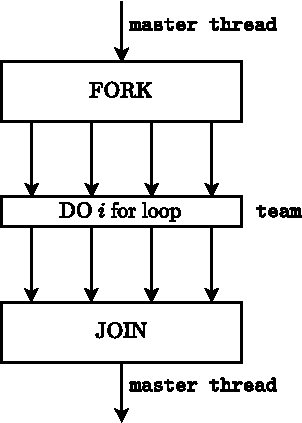
\includegraphics[width=.3\textwidth]{img/openmp-for-1.pdf}
    \caption{OpenMP for loop.}
\end{figure}

\noindent
\begin{openmpbox}[: \texttt{pragma omp for}]
\begin{lstlisting}[language=C++]
#pragma omp parallel
{
    #pragma omp for
    /* for loop */
}\end{lstlisting}
\end{openmpbox}

\noindent
The for directive parallelize execution of iterations. The number of iteration cannot be internally modified. Some common clauses are:
\begin{itemize}
    \item \texttt{\emph{schedule}} that describes \textbf{how iterations of the loop are distributed among the threads in the team}. The schedule type can be either \texttt{dynamic}, \texttt{guided}, \texttt{runtime}, or \texttt{static}.
    \begin{itemize}
        \item \texttt{\emph{static}}. Loop \textbf{iterations are divided into blocks of size \texttt{chunk}} and then statically allocated to threads. If \texttt{chunk} is \textbf{\underline{not} specified}, the \textbf{iterations are divided evenly} (if possible) \textbf{among the threads}.
        \newpage
        \begin{openmpbox}[: \texttt{static schedule}]
\begin{lstlisting}[language=C++, mathescape=true]
#pragma omp for schedule(static, $\emph{chunk-size}$)\end{lstlisting}
        \end{openmpbox}
        \begin{figure}[!htp]
            \centering
            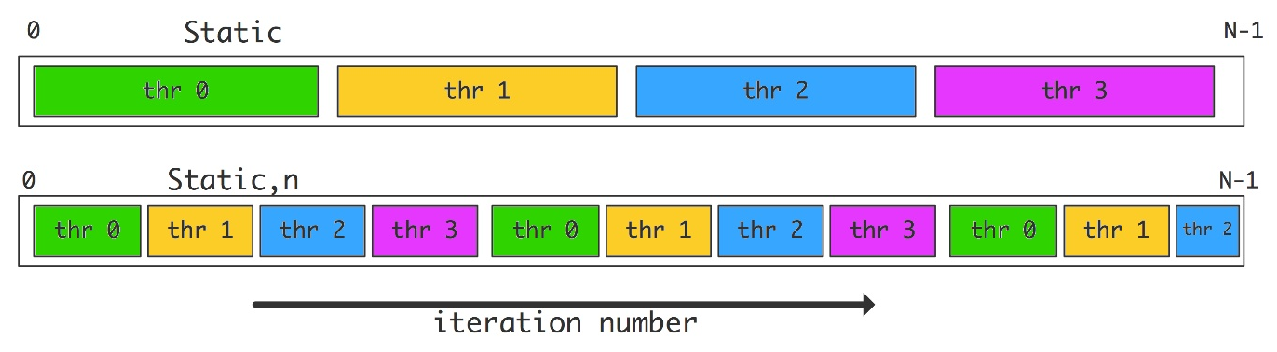
\includegraphics[width=\textwidth]{img/openmp-for-2.pdf}
            \caption{\texttt{static} schedule.}
        \end{figure}

        \item \texttt{\emph{dynamic}}. Loop \textbf{iterations are divided into blocks of size \texttt{chunk}} and \textbf{distributed among the threads \emph{at runtime}}; when a thread completes one chunk, it is \textbf{dynamically allocated another}. The default chunk size is 1. In fact, we can see in the image that the order is not always the same.
        \begin{openmpbox}[: \texttt{dynamic schedule}]
\begin{lstlisting}[language=C++, mathescape=true]
#pragma omp for schedule(dynamic, $\emph{chunk-size}$)\end{lstlisting}
        \end{openmpbox}
        \begin{figure}[!htp]
            \centering
            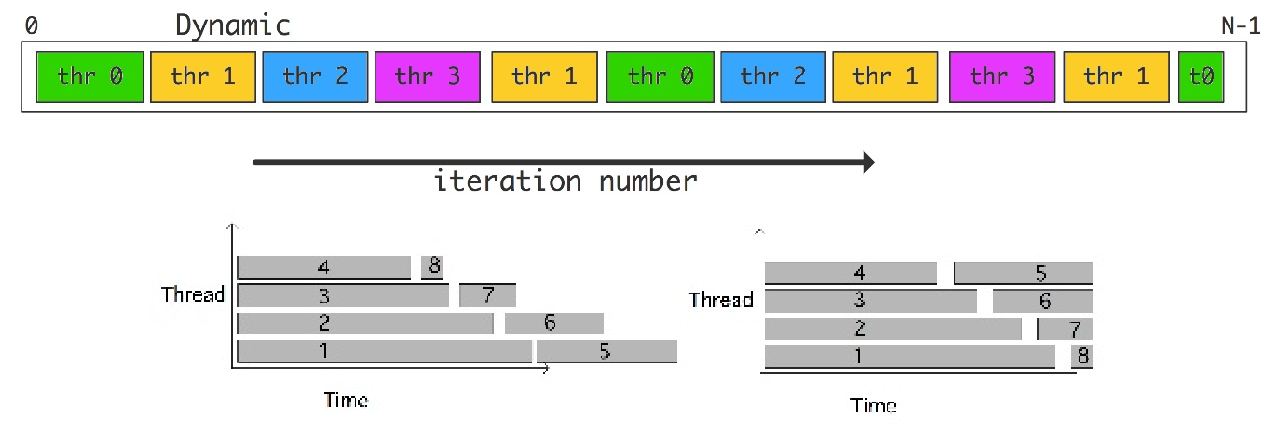
\includegraphics[width=\textwidth]{img/openmp-for-3.pdf}
            \caption{\texttt{dynamic} schedule.}
        \end{figure}
        
        \item \texttt{\emph{runtime}}. Depends on environment variable \texttt{OMP\_SCHEDULE}.

        \item \texttt{\emph{guided}}. Static, gradually decreases the chunk size (\texttt{chunk} specifies the smallest one).
        \begin{openmpbox}[: \texttt{guided schedule}]
\begin{lstlisting}[language=C++, mathescape=true]
#pragma omp for schedule(guided)\end{lstlisting}
        \end{openmpbox}
        \begin{figure}[!htp]
            \centering
            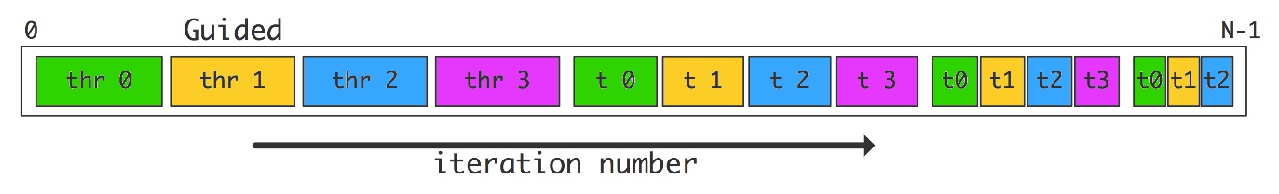
\includegraphics[width=\textwidth]{img/openmp-for-4.pdf}
            \caption{\texttt{guided} schedule.}
        \end{figure}
    \end{itemize}
    \begin{examplebox}[: \texttt{schedule} types]
\begin{lstlisting}[language=C++]
#include <stdio.h>
#include <omp.h>

#define NUM_THREADS 4
#define STATIC_CHUNK 5
#define DYNAMIC_CHUNK 5
#define NUM_LOOPS 20
#define SLEEP_EVERY_N 3

int main( )
{
    int nStatic1[NUM_LOOPS],
        nStaticN[NUM_LOOPS];
    int nDynamic1[NUM_LOOPS],
        nDynamicN[NUM_LOOPS];
    int nGuided[NUM_LOOPS];

    omp_set_num_threads(NUM_THREADS);

    #pragma omp parallel
    {
        #pragma omp for schedule(static, 1)
        for (int i = 0 ; i < NUM_LOOPS ; ++i)
        {
            if ((i % SLEEP_EVERY_N) == 0)
                Sleep(0);
            nStatic1[i] = omp_get_thread_num( );
        }

        #pragma omp for schedule(static, STATIC_CHUNK)
        for (int i = 0 ; i < NUM_LOOPS ; ++i)
        {
            if ((i % SLEEP_EVERY_N) == 0)
                Sleep(0);
            nStaticN[i] = omp_get_thread_num( );
        }

        #pragma omp for schedule(dynamic, 1)
        for (int i = 0 ; i < NUM_LOOPS ; ++i)
        {
            if ((i % SLEEP_EVERY_N) == 0)
                Sleep(0);
            nDynamic1[i] = omp_get_thread_num( );
        }

        #pragma omp for schedule(dynamic, DYNAMIC_CHUNK)
        for (int i = 0 ; i < NUM_LOOPS ; ++i)
        {
            if ((i % SLEEP_EVERY_N) == 0)
                Sleep(0);
            nDynamicN[i] = omp_get_thread_num( );
        }

        #pragma omp for schedule(guided)
        for (int i = 0 ; i < NUM_LOOPS ; ++i)
        {
            if ((i % SLEEP_EVERY_N) == 0)
                Sleep(0);
            nGuided[i] = omp_get_thread_num( );
        }
    }

    printf_s("------------------------------------------------\n");
    printf_s("| static | static | dynamic | dynamic | guided |\n");
    printf_s("|    1   |    %d   |    1    |    %d    |        |\n",
                STATIC_CHUNK, DYNAMIC_CHUNK);
    printf_s("------------------------------------------------\n");

    for (int i=0; i<NUM_LOOPS; ++i)
    {
        printf_s("|    %d   |    %d   |    %d    |    %d    |"
                    "    %d   |\n",
                    nStatic1[i], nStaticN[i],
                    nDynamic1[i], nDynamicN[i], nGuided[i]);
    }

    printf_s("------------------------------------------------\n");
}\end{lstlisting}
    The result will be:
\begin{lstlisting}
------------------------------------------------
| static | static | dynamic | dynamic | guided |
|    1   |    5   |    1    |    5    |        |
------------------------------------------------
|    0   |    0   |    0    |    2    |    1   |
|    1   |    0   |    3    |    2    |    1   |
|    2   |    0   |    3    |    2    |    1   |
|    3   |    0   |    3    |    2    |    1   |
|    0   |    0   |    2    |    2    |    1   |
|    1   |    1   |    2    |    3    |    3   |
|    2   |    1   |    2    |    3    |    3   |
|    3   |    1   |    0    |    3    |    3   |
|    0   |    1   |    0    |    3    |    3   |
|    1   |    1   |    0    |    3    |    2   |
|    2   |    2   |    1    |    0    |    2   |
|    3   |    2   |    1    |    0    |    2   |
|    0   |    2   |    1    |    0    |    3   |
|    1   |    2   |    2    |    0    |    3   |
|    2   |    2   |    2    |    0    |    0   |
|    3   |    3   |    2    |    1    |    0   |
|    0   |    3   |    3    |    1    |    1   |
|    1   |    3   |    3    |    1    |    1   |
|    2   |    3   |    3    |    1    |    1   |
|    3   |    3   |    0    |    1    |    3   |
------------------------------------------------\end{lstlisting}
    \end{examplebox}

    \item \texttt{\emph{nowait}} to \textbf{avoid synchronization at the end of the parallel loop}. It overrides the barrier implicit in a directive.
    \begin{lstlisting}[language=C++]
#pragma omp for nowait\end{lstlisting}
    \begin{examplebox}[: \texttt{nowait} clause]
\begin{lstlisting}[language=C++]
#include <stdio.h>

#define SIZE 5

void test(int *a, int *b, int *c, int size)
{
    int i;
    #pragma omp parallel
    {
        #pragma omp for nowait
        for (i = 0; i < size; i++)
            b[i] = a[i] * a[i];

        #pragma omp for nowait
        for (i = 0; i < size; i++)
            c[i] = a[i]/2;
    }
}

int main( )
{
    int a[SIZE], b[SIZE], c[SIZE];
    int i;

    for (i=0; i<SIZE; i++)
        a[i] = i;

    test(a,b,c, SIZE);

    for (i=0; i<SIZE; i++)
        printf_s("%d, %d, %d\n", a[i], b[i], c[i]);
}\end{lstlisting}
    The output will be:
\begin{lstlisting}
0, 0, 0
1, 1, 0
2, 4, 1
3, 9, 1
4, 16, 2\end{lstlisting}
    \end{examplebox}
\end{itemize}

\newpage

\paragraph{Reduction}\label{paragraph: Reduction}

\noindent
In parallel programming, sometimes there are some exceptional cases when we use the \texttt{for} statement where the variables inside the code block are not so easy to manage (memory viewpoint). For example, consider the following case:
\begin{center}
\begin{lstlisting}[language=C++]
#include "stdio.h"
#include "omp.h"
#define MAX 10


int main(int argc, char const *argv[])
{
    double ave = 0.0;
    double A[MAX] = {1, 2, 3, 4, 5, 6, 7, 8, 9, 10};
    int i;
    #pragma omp parallel for
    for(i = 0; i < MAX; i++) {
        ave += A[i];
    }
    ave = ave / MAX;
    printf("Value %f\n", ave);
    return 0;
}
\end{lstlisting}
\textcolor{Red2}{\faIcon{exclamation-triangle} \textbf{Too many threads modifying the same variable}}
\end{center}
In this case, we are combining values into a single accumulation variable (called \texttt{ave}). There is a true dependence between loop iterations that can't be trivially removed. A \textbf{continuous execution produces different results!}
\begin{lstlisting}[language=bash, mathescape=false]
$ ./example.out
Value 1.300000
$ ./example.out
Value 2.400000
$ ./example.out 
Value 2.500000
$ ./example.out 
Value 2.100000
$ ./example.out 
Value 1.900000    
\end{lstlisting}
This is a very common situation and a solution, which can also be \textbf{used as a synchronization technique}, is called a \textbf{reduction}.

\highspace
A reduction variable in a loop \textbf{aggregates} (i.e., accumulates) a \textbf{value that depends on each iteration of the loop} and \textbf{doesn't depend on the iteration order}.

\begin{openmpbox}[: \texttt{reduction}]
    \begin{lstlisting}[language=C++, mathescape=true]
#pragma omp parallel for reduction($\emph{operator}$: $\emph{list}$)\end{lstlisting}
\end{openmpbox}

\noindent
A reduction clause:
\begin{itemize}
    \item It \textbf{makes a local copy} of each \texttt{\emph{list}} variable and initialized depending on the \texttt{\emph{operator}};
    \item It \textbf{updates occur on the local copy};
    \item \textbf{Local copies are reduced into a single value and combined with the original global value}.
\end{itemize}
Therefore, the variables in \texttt{\emph{list}} must be shared in the enclosing parallel region.

\highspace
Many different associative operands (\texttt{\emph{operator}} value) can be used with reduction:
\begin{itemize}
    \item \texttt{+} with initial value 0
    \item \texttt{*} with initial value 1
    \item \texttt{-} with initial value 0
    \item \texttt{min} with initial value as largest positive number
    \item \texttt{max} with initial value as most negative number
    \item \texttt{\&} with initial value $\sim0$
    \item \texttt{|} with initial value 0
    \item \texttt{\textasciicircum} with initial value 0
    \item \texttt{\&\&} with initial value 1
    \item \texttt{||} with initial value 0
\end{itemize}
Using the \texttt{reduction} clause, the code written at the beginning of the paragraph can be fixed as follows:
\begin{center}
\begin{lstlisting}[language=C++]
#include "stdio.h"
#include "omp.h"
#define MAX 10


int main(int argc, char const *argv[])
{
    double ave = 0.0;
    double A[MAX] = {1, 2, 3, 4, 5, 6, 7, 8, 9, 10};
    int i;
    // use reduction
    #pragma omp parallel for reduction(+: ave)
    for(i = 0; i < MAX; i++) {
        ave += A[i];
    }
    ave = ave / MAX;
    // now it prints the correct result 5.5
    printf("Value %f\n", ave);
    return 0;
}
\end{lstlisting}
\textcolor{Green3}{\faIcon{check} \textbf{Avoid race condition}}
\end{center}

    \subsubsection{Sections}

\textbf{Section} identifies code \textbf{sections to be divided among all threads}.

\highspace
Sections allow to specify that the enclosed section(s) of code are to be executed in parallel. \textbf{Each section is executed once by a thread in the team}.

\marginpar{
    \href{https://www.openmp.org/spec-html/5.0/openmpsu37.html\#x59-1010002.8.1} {Doc. \faIcon{book}}
}
\begin{openmpbox}[: sections]
\begin{lstlisting}[language=C++]
#pragma omp [parallel] sections [clauses]
{
    #pragma omp section
    {
        code_block
    }
}\end{lstlisting}
\end{openmpbox}

\noindent
The sections directive identifies a noniterative work-sharing construct that specifies a set of constructs that are to be divided among threads in a team. Each section is executed once by a thread in the team.

\highspace
Each section is preceded by a \texttt{section} directive, although the \texttt{section} directive is optional for the first section. The \texttt{section} directives must appear within the lexical extent of the \texttt{sections} directive. There's an \textbf{implicit barrier} at the end of a \texttt{sections} construct, unless a \texttt{nowait} is specified.

\highspace
Restrictions to the sections directive are as follows:
\begin{itemize}
    \item A \texttt{section} directive must not appear outside the lexical extent of the \texttt{sections} directive.
    \item Only a single \texttt{nowait} clause can appear on a \texttt{sections} directive.
\end{itemize}

\begin{figure}[!htp]
    \centering
    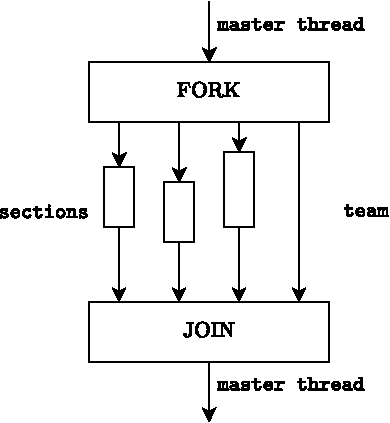
\includegraphics[width=.45\textwidth]{img/openmp-sections-1.pdf}
    \caption{Breaks work into separate, discrete sections, each executed by a thread (functional parallelism).}
\end{figure}

    \subsubsection{Single/Master}

A \textbf{section} (not the directive) \textbf{of code should be executed on a single thread, not necessarily the main (master) thread}. The \texttt{single} directive identifies a construct that specifies that the associated structured block is executed by only one thread in the team (not necessarily the master thread).

\begin{openmpbox}[: \texttt{single} and \texttt{master}]
\begin{lstlisting}[language=C++]
#pragma omp parallel
{
    #pragma omp single
    {
        /* code section */
    }
    # pragma omp master
    {
        /* code section */
    }
}\end{lstlisting}
\end{openmpbox}

\begin{itemize}
    \item \texttt{single} specifies that a section of a code is \textbf{executed only by a single thread}.\marginpar{
        \href{https://www.openmp.org/spec-html/5.0/openmpsu38.html\#x60-1090002.8.2} {Doc. \faIcon{book}}
    }

    
    \item \texttt{master} specifies that a section of a code is \textbf{executed only by the master}.\marginpar{
        \href{https://www.openmp.org/spec-html/5.0/openmpse24.html\#x118-4380002.16} {Doc. \faIcon{book}}
    }
\end{itemize}

\noindent
There's an \textbf{implicit barrier} after the \texttt{single} construct unless a \texttt{nowait} clause is specified.

    \subsubsection{Tasks}

The following section has been enhanced with slides from Senior Principal Engineer Mattson Tim. He's a senior principal engineer at Intel, where he's been since 1993. His profile can be seen \href{https://www.intel.com/content/www/us/en/research/featured-researchers/tim-mattson.html}{here} and the slides are available online \href{https://www.openmp.org/wp-content/uploads/Intro_To_OpenMP_Mattson.pdf}{here}. He has also made an interesting \href{https://youtube.com/playlist?list=PLLX-Q6B8xqZ8n8bwjGdzBJ25X2utwnoEG&si=OBjyY4AI4zWfA-vB}{YouTube series} on the introduction to OpenMP.

\highspace
Tasks are \textbf{independent units of work}. They consist of: \emph{code to execute}, \emph{data environment}, and \emph{internal control variables} (ICV). \textbf{Threads perform the work of each task}. The runtime \textbf{system decides when to execute tasks}; each task can be deferred or executed immediately.

\highspace
In other words, an OpenMP \textbf{task is a block of code contained in a parallel region that can be executed simultaneously with other tasks in the same region}.

\highspace
Some useful terminology:
\begin{itemize}
    \item \textbf{\emph{Task construct}}. It identifies the \textbf{task directive plus the structured block}.
    
    \item \textbf{\emph{Task}}. It is the \textbf{package of code and instructions} for \textbf{allocating data} created when a \textbf{thread encounters a task construct}.
    
    \item \textbf{\emph{Task region}}. It is the dynamic sequence of \textbf{instructions generated by the execution of a task by a thread}.
\end{itemize}
Tasks are guaranteed to complete at thread barriers (using the \texttt{barrier} directive) or at task barriers (using the \texttt{taskwait} directive):
\begin{lstlisting}[language=C++, mathescape=true]
#pragma omp parallel // omp directive to parallel the code
{
    #pragma omp task // multiple $\textcolor{codegreen}{\emph{foo}}$ tasks created here, 
                     // one for each thread
    foo();
    #pragma omp barrier // all $\textcolor{codegreen}{\emph{foo}}$ tasks guaranteed 
                        // to be completed here
    #pragma omp single  // only one thread can access to 
                        // this piece of code
    {
        #pragma omp task // one $\textcolor{codegreen}{\emph{bar}}$ task created here
        bar();
    }
    // $\textcolor{codegreen}{\emph{foo}}$ task guaranteed to be completed here
}
\end{lstlisting}
\begin{examplebox}[: Fibonacci with tasks]
    Let us see a Fibonacci example of data scoping using the tasks. In the following code, we create the Fibonacci function and we create two tasks, but each task has a private variable and these variables are also used in the return statement:
    \begin{lstlisting}[language=C++]
int fib(int n) {
    int x, y;
    if(n < 2)
        return n;
    #pragma omp task
    x = fib(n-1);
    #pragma omp task
    y = fib(n-2);
    #pragma omp taskwait
    return x + y;
}\end{lstlisting}
    A good solution is to \dquotes{share} the \texttt{x} and \texttt{y} variables because we need both values to calculate the sum.
    \begin{lstlisting}[language=C++]
int fib(int n) {
    int x, y;
    if(n < 2)
        return n;
    #pragma omp task shared(x)
    x = fib(n-1);
    #pragma omp task shared(y)
    y = fib(n-2);
    #pragma omp taskwait
    return x + y;
}\end{lstlisting}
\end{examplebox}

\begin{flushleft}
    \textcolor{Green3}{\faIcon{check} \textbf{Main advantage}}
\end{flushleft}
Note the following code:
\begin{lstlisting}[language=C++]
// create a team of threads
#pragma omp parallel
{
    // one thread executes the single construct
    // and other threads wait at the implied 
    // barrier at the end of the single construct
    #pragma omp single
    { // block 1
        node *p = head;
        while(p) { // block 2
            // the single thread creates a task
            // with its own value for the pointer p
            #pragma omp task firstprivate(p)
                process(p);
            p = p -> next; // block 3
        }
        // execution moves beyond the barrier 
        // once all the tasks are complete
    }
}
\end{lstlisting}
The tasks have the \textbf{potential to parallelize irregular patterns and recursive function calls}. See Figure \ref{figure: openmp tasks 1} (page \pageref{figure: openmp tasks 1}) to understand how the runtime system can optimize execution using the tasks.
\begin{figure}[!htp]
    \centering
    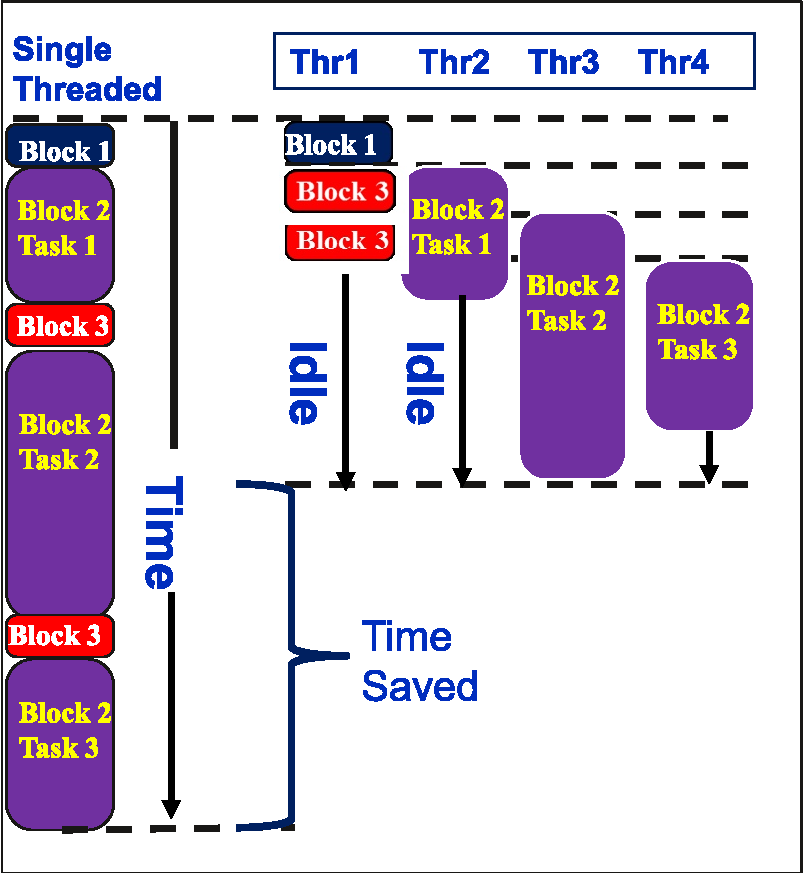
\includegraphics[width=.6\textwidth]{img/openmp-tasks-1.pdf}
    \caption{The main advantage of the tasks is to parallelize irregular patterns and recursive function calls.}
    \label{figure: openmp tasks 1}
\end{figure}

\newpage

\begin{flushleft}
    \textcolor{Green3}{\faIcon{bookmark} \textbf{Synchronization}}
\end{flushleft}
When a thread encounters a \texttt{task} construct, the task is created but not immediately executed. The tasks are guaranteed to be completed:
\begin{itemize}
    \item At a \textbf{barrier} (implicit or explicit)
    \item At \textbf{task synchronization points}:
    \begin{itemize}
        \item \texttt{taskwait} construct specifies a \textbf{wait on the completion of child tasks of the current task}.
        \marginpar{
            \href{https://www.openmp.org/spec-html/5.0/openmpsu94.html} {Doc. \faIcon{book}}
        }
        \begin{openmpbox}[: \texttt{pragma omp taskwait}]
        \begin{lstlisting}[language=C++]
#pragma omp taskwait\end{lstlisting}
        \end{openmpbox}

        \item \texttt{taskgroup} construct specifies a \textbf{wait on the completion of child tasks of the current task} (such as \texttt{taskwait}) and \textbf{their descendent tasks} (\underline{main difference}).
        \marginpar{
            \href{https://www.openmp.org/spec-html/5.0/openmpsu93.html\#x124-4690002.17.5} {Doc. \faIcon{book}}
        }
        \begin{openmpbox}[: \texttt{pragma omp taskgroup}]
        \begin{lstlisting}[language=C++]
#pragma omp taskgroup\end{lstlisting}
        \end{openmpbox}
    \end{itemize}
\end{itemize}

    \paragraph{Task dependences}

By creating tasks instead of sections, each thread can execute any task as long as its input is ready. Since the internal scheduler decides how to manipulate the execution of tasks, there is a useful \textbf{clause to indicate a dependency between tasks}.
\marginpar{
    \href{https://www.openmp.org/spec-html/5.0/openmpsu99.html} {Doc. \faIcon{book}}
}
\begin{openmpbox}[: \texttt{depend}]
    \begin{lstlisting}[language=C++, mathescape=true]
#pragma omp task depend($\emph{dependence-type}$: variable)\end{lstlisting}
    The \texttt{depend} clause enforces additional constraints on the scheduling of tasks or loop iterations. These constraints establish dependencies only between sibling tasks or between loop iterations.

    The \emph{dependence-type} can be \texttt{in} or \texttt{out}.
\end{openmpbox}

\noindent
In addition to the depend clause, we can also use the priority clause to hint that more important tasks should be executed more frequently.

\highspace
The \texttt{priority} clause is a \textbf{hint for the priority of the generated task}. The priority-value is a \textbf{non-negative integer expression} that provides a hint for task execution order. Among all tasks ready to be executed, \textbf{higher priority tasks} (those with a higher numerical value in the priority clause expression) \textbf{are recommended to execute before lower priority ones}. The \textbf{default} priority-value when no priority clause is specified \textbf{is zero} (the \emph{lowest priority}).

\highspace
\textbf{If a value is specified in the priority clause that is higher than the \emph{max-task-priority-var}} ICV (internal control variables) then the implementation will \textbf{use the value of that ICV}. A program that relies on task execution order being determined by this priority-value may have unspecified behavior.
\begin{itemize}
    \item The \texttt{omp\_get\_max\_task\_priority} routine returns the \textbf{maximum value that can be specified in the \texttt{priority} clause}.
    \marginpar{
        \href{https://www.openmp.org/spec-html/5.0/openmpsu151.html\#x188-8880003.2.42} {Doc. \faIcon{book}}
    }
    \begin{openmpbox}[: \texttt{omp\_get\_max\_task\_priority}]
        \begin{lstlisting}[language=C++]
int omp_get_max_task_priority()\end{lstlisting}
    \end{openmpbox}

    \item The \texttt{OMP\_MAX\_TASK\_PRIORITY} environment variable \textbf{controls the use of task priorities} by setting the initial value of the \emph{max-task-priority-var} ICV. The value of this environment variable must be a non-negative integer.\marginpar{
        \href{https://www.openmp.org/spec-html/5.0/openmpse64.html\#x303-20810006.16} {Doc. \faIcon{book}}
    }
\end{itemize}

\begin{flushleft}
    \textcolor{Red2}{\faIcon{exclamation-triangle} \textbf{Possible overhead}}
\end{flushleft}
The task in general, but especially the \textbf{dependencies between tasks, can introduce overhead and reduce performance}.

\newpage

\begin{examplebox}[: dependences]
    Let the following parallel code:
    \begin{lstlisting}[language=C++, mathescape=true]
#pragma omp parallel default(none) \
                     shared(fp_read) \
                     shared(n_io_chunks) \
                     shared(n_work_chunks) \
                     shared(a, b, c) \
                     shared(status_read, status_processing) \
                     shared(status_postprocessing)
{
    #pragma omp single nowait
    {
        for(int64_t i = 0; i < n_io_chunks; ++i) {
            #pragma omp task depend(out: status_read[i]) \
                             priority(20)
            {
                (void) read_input(
                    fp_read, i, a, b, &status_read[i]
                );
            } // End of task reading in a chunk of data

            #pragma omp task depend(in: status_read[i]) \
                        depend(out: status_processing[i]) \
                        priority(10)
            {
                (void) compute_results(
                    i, n_work_chunks, a, b, c,
                    &status_processing[i]
                );
            } // End of task performing the computations

            #pragma omp task depend(in: status_processing[i])
                             priority(5)
            {
                (void) postprocess_results(
                    i, n_work_chunks, c,
                    &status_postprocessing[i]
                );
            } // End of task postprocessing the results
        } // End of for-loop
    } // End of single region
} // End of parallel region
    \end{lstlisting}
    \begin{itemize}
        \item Row 11. We are going to process \texttt{n\_io\_chunks} of data.
        \item Rows 12, 20. Refer to read and are compute dependence.
        \item Rows 21, 30. Refer to compute and are postprocess dependence.
    \end{itemize}
    \newpage
    A possible order of execution if we consider 3 threads is:
    \begin{center}
        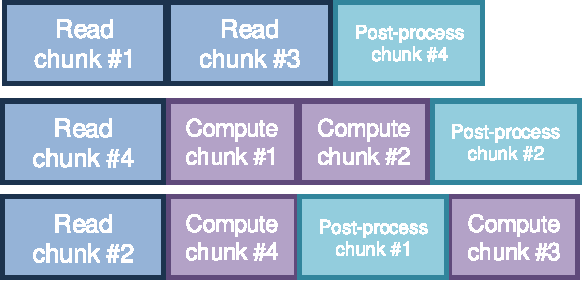
\includegraphics[width=.6\textwidth]{img/task-dependence-1.pdf}
    \end{center}
    As long as the dependencies are respected, the loop iterations can be executed in any order. No explicit \texttt{flush} (page \hyperlink{openmp: flush}{\hypergetpageref{openmp: flush}}) are required because it is implied before and after every task.
\end{examplebox}

\begin{flushleft}
    \textcolor{Green3}{\faIcon{question-circle} \textbf{Custom number of iterations}}
\end{flushleft}
\textbf{Each task gets assigned a number of iterations which is the minimum between \texttt{grainsize} and the total number of iterations}.

\highspace
If a \texttt{grainsize} clause is present, the number of logical iterations assigned to each generated task is greater than or equal to the minimum of the value of the \texttt{\emph{grain-size}} expression and the number of logical iterations, but less than two times the value of the \texttt{\emph{grain-size}} expression.

\highspace
If the \texttt{grainsize} clause has the \texttt{\emph{strict}} modifier, the number of logical iterations assigned to each generated task is equal to the value of the \texttt{\emph{grain-size}} expression, except for the generated task that contains the sequentially last iteration, which may have fewer iterations. The parameter of the \texttt{grainsize} clause must be a positive integer expression.
\marginpar{
    \href{https://www.openmp.org/spec-html/5.1/openmpsu55.html} {Doc. \faIcon{book}}
}
\begin{openmpbox}[: \texttt{pragma omp taskloop grainsize}]
    \begin{lstlisting}[language=C++, mathescape=true]
#pragma omp taskloop grainsize($\emph{[strict] grain-size}$)\end{lstlisting}
\end{openmpbox}

\newpage

\begin{flushleft}
    \textcolor{Green3}{\faIcon{question-circle} \textbf{Number of created tasks}}
\end{flushleft}
\textbf{To keep the number of created tasks low, the clause \texttt{num\_tasks} sets the number of tasks that the runtime system can generate}.

\highspace
If \texttt{num\_tasks} is specified, the \texttt{taskloop} construct creates as many tasks as the minimum of the \texttt{\emph{num-tasks}} expression and the number of logical iterations. Each task must have at least one logical iteration. The parameter of the \texttt{num\_tasks} clause must be a positive integer expression.

\highspace
If the \texttt{num\_tasks} clause has the \texttt{\emph{strict}} modifier for a task loop with $N$ logical iterations, the logical iterations are partitioned in a balanced manner and each partition is assigned, in order, to a generated task. The partition size is $\left\lceil\left\lceil \dfrac{N}{\texttt{\emph{num-tasks}}} \right\rceil \right\rceil$ until the number of remaining iterations divides the number of remaining tasks evenly, at which point the partition size becomes $\left\lfloor\left\lfloor \dfrac{N}{\texttt{\emph{num-tasks}}} \right\rfloor\right\rfloor$.
\marginpar{
    \href{https://www.openmp.org/spec-html/5.1/openmpsu55.html} {Doc. \faIcon{book}}
}
\begin{openmpbox}[: \texttt{pragma omp taskloop num\_tasks}]
    \begin{lstlisting}[language=C++, mathescape=true]
#pragma omp taskloop num_tasks($\emph{[strict] num-tasks}$)\end{lstlisting}
\end{openmpbox}

\highspace
\textbf{If neither a \texttt{grainsize} nor \texttt{num\_tasks} clause is present, the number of loop tasks generated and the number of logical iterations assigned to these tasks is implementation defined.}
    \subsection{Synchronization}

The following section has been enhanced with slides from Senior Principal Engineer Mattson Tim. He's a senior principal engineer at Intel, where he's been since 1993. His profile can be seen \href{https://www.intel.com/content/www/us/en/research/featured-researchers/tim-mattson.html}{here} and the slides are available online \href{https://www.openmp.org/wp-content/uploads/Intro_To_OpenMP_Mattson.pdf}{here}. He has also made an interesting \href{https://youtube.com/playlist?list=PLLX-Q6B8xqZ8n8bwjGdzBJ25X2utwnoEG&si=OBjyY4AI4zWfA-vB}{YouTube series} on the introduction to OpenMP.

\highspace
OpenMP is a multi-threaded, shared address model. This means that threads communicate by sharing variables. Unfortunately, this can cause some problems such as race conditions (page \pageref{def: race condition}). The solution is to \textbf{use synchronization to protect against data conflicts}. The good news is that synchronization can avoid data race problems, but it is also an \textbf{expensive method}. So we can use synchronization, but we \textbf{need to change the way data is accessed to minimize the need for synchronization}.

\highspace
Synchronization brings \textbf{one or more threads to a well-defined and known point in their execution}. The two most common forms of synchronization are:
\begin{itemize}
    \item \textbf{\emph{Barrier}}: each thread wait at the barrier \textbf{until all threads arrive}.
    \item \textbf{\emph{Mutual exclusion}}: define a block of code that \textbf{only one thread at a time can execute}.
\end{itemize}
The OpenMP directives are: \texttt{critical}, \texttt{atomic}, and \texttt{barrier}. These are high-level synchronization directives, but there are also low-level synchronization directives, such as \texttt{flush} and \texttt{locks}, but they are too complex at the moment, we will see them later.

\begin{figure}[!htp]
    \centering
    \begin{subfigure}{.45\textwidth}
        \centering
        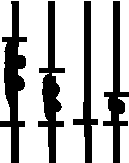
\includegraphics[width=.25\textwidth]{img/openmp-sync-1.pdf}
        \caption{Barrier. Each thread wait at the barrier until all threads arrive.}
    \end{subfigure}
    \hfill
    \begin{subfigure}{.45\textwidth}
        \centering
        
\includegraphics[width=.25\textwidth]{img/openmp-sync-2.pdf}
        \caption{Mutual exclusion. Define a block of code that only one thread at a time can execute.}
    \end{subfigure}
\end{figure}

\newpage

\noindent
\textbf{\underline{Barrier}}. Each thread waits until all threads arrive.
\begin{openmpbox}[: \texttt{barrier}]
    \begin{lstlisting}[language=C++, mathescape=true]
#pragma omp barrier $\emph{name}$\end{lstlisting}
\end{openmpbox}

\noindent
An \underline{optional} \texttt{name} may be used to identify the \texttt{critical} region. A \textbf{thread waits at the beginning of a critical region} until no other thread is executing a critical region (anywhere in the program) \textbf{with the same name}. \textbf{All unnamed \texttt{critical} directives map to the same unspecified name}.

\begin{examplebox}[: synchronization with \texttt{barrier} directive]
    The following example includes several critical directives. The example illustrates a queuing model in which a task is dequeued and worked on. To guard against many threads dequeuing the same task, the dequeuing operation must be in a \texttt{critical} section. Because the two queues in this example are independent, they're protected by \texttt{critical} directives with different names, \emph{xaxis} and \emph{yaxis}.\cite{openMPCriticalDirectiveMicrosoftExample}
    \begin{lstlisting}[language=C++]
#pragma omp parallel shared(x, y) private(x_next, y_next)
{
    #pragma omp critical ( xaxis )
        x_next = dequeue(x);
    work(x_next);
    #pragma omp critical ( yaxis )
        y_next = dequeue(y);
    work(y_next);
}
    \end{lstlisting}
\end{examplebox}

\highspace
\textbf{\underline{Mutual exclusion}}. Only one thread at a time can enter a \emph{critical} region.
\begin{openmpbox}[: \texttt{critical}]
    \begin{lstlisting}[language=C++]
#pragma omp critical\end{lstlisting}
\end{openmpbox}
\begin{table}[!htp]
    \centering
    \begin{tabular}{@{} p{8em} | p{12em} | p{12em} @{}}
        \toprule
        & \texttt{omp critical} & \texttt{omp single} \\
        \midrule
        Meaning & Run code segment one by one by all threads & Run code segment once by any thread \\
        \cmidrule{1-3}
        Number of times code is executed & Number of threads & Only one \\
        \cmidrule{1-3}
        Use case & Avoid race condition & Manage control variables or signals \\
        \bottomrule
    \end{tabular}
    \caption{\textcolor{Red2}{\faIcon{exclamation-triangle} \textbf{\texttt{omp critical} vs \texttt{omp single}}}}
\end{table}
\begin{examplebox}[: synchronization with \texttt{critical} directive]
    Note the following code:
    \begin{lstlisting}[language=C++, mathescape=true]
float res;

#pragma omp parallel
{
    float B;
    int i, id, nthrds, niters = $\emph{big\_number}$;

    id = omp_get_thread_num();
    nthrds = omp_get_num_threads();
    for (i = id; i < niters; i += nthrds) {
        B = big_job(i);
        #pragma omp critical // threads wait their turn;
        res += consume(B);   // only one at a time
    }                        // calls consume
}
    \end{lstlisting}
\end{examplebox}

\highspace
\textbf{\underline{Atomic}}. Provides mutual exclusion, but only when updating a memory location. It \textbf{ensures that a particular memory location is accessed atomically}. It is \textbf{valid only for the following statement} and not for a structured block.

\highspace
The statement inside the atomic must be one of the following forms:
\begin{itemize}
    \item \texttt{x binop = expr}
    \item \texttt{x++} or \texttt{++x}
    \item \texttt{x-}\texttt{-} or \texttt{-}\texttt{-x}
\end{itemize}
Where \texttt{x} is an lvalue of scalar type and \texttt{binop} is a non-overloaded builtin operator.

\begin{openmpbox}[: \texttt{atomic}]
    \begin{lstlisting}[language=C++]
#pragma omp atomic\end{lstlisting}
\end{openmpbox}

\begin{examplebox}[: synchronization with \texttt{atomic} directive]
    \begin{lstlisting}[language=C++]
#pragma omp parallel
{
    double tmp, B;
    B = DOIT();
    tmp = big_ugly(B);
    #pragma omp atomic
    X += tmp;
}
    \end{lstlisting}
\end{examplebox}
    \subsection{Data environment}\label{subsection: Data environment}

OpenMP is based on the shared memory programming model, so most \textbf{variables are shared by default}. \textbf{Global variables are also shared between threads}. But not everything is shared; for example, \emph{stack variables} in functions called from parallel regions are \textbf{private}, as are \emph{automatic variables} within a statement block.

\begin{examplebox}[: data sharing]
    In the following code, the variable \texttt{temp} is private (local to each thread) because it is in the stack of the function \texttt{work}; meanwhile, the variables \texttt{A}, \texttt{index}, and \texttt{count} are shared by all threads.
    \begin{lstlisting}[language=C++]
double A[10];
int main() {
    int index[10];
    #pragma omp parallel
        work(index);
    printf("%d\n", index[0]);
}

void work(int *index) {
    double temp[10];
    static int count;
    /* other code */
}\end{lstlisting}
\end{examplebox}

\noindent
We can refer to these arguments as \textbf{Data Scope Attribute Clauses} because the issue is really about the visibility and value of each data in each scope. Although OpenMP shares variables by default, there is (and it is a very common and \emph{best practice}) the option to:
\begin{itemize}
    \item Selectively \textbf{change storage attributes for construct} using the following clauses: \texttt{shared}, \texttt{private} and \texttt{firstprivate}.
    \item The \textbf{final value} of a private inside a parallel loop can be \textbf{transmitted to the shared variable outside the loop} with: \texttt{lastprivate}.
    \item The \textbf{default attributes can be overridden} with:
    \vspace{-.8em}
    \begin{center}
        \texttt{default(private | shared | none)}
    \end{center}
    \vspace{-.8em}
\end{itemize}
\textcolor{Red2}{\faIcon{exclamation-triangle} \textbf{Note that when we say \dquotes{copy} we mean the \emph{shallow copy}, not the \emph{deep copy}. So when the following clauses create a local copy, they create a \emph{shallow copy}.}}

\highspace
\textbf{\underline{\texttt{private} clause}}. The statement \texttt{private(var)} creates a \textbf{new local copy} of \texttt{var} \textbf{for each thread}. The value of the private copies is \textbf{\emph{uninitialized}} and also the \textbf{original variable value remains unchanged after the region}.
\begin{openmpbox}[: \texttt{private(\emph{...})}]
    \begin{lstlisting}[language=C++, mathescape=true]
#pragma omp parallel $\emph{directive}$ private($\emph{var1-name}$, $\emph{var2-name}$, ...)\end{lstlisting}
\end{openmpbox}
\begin{examplebox}[: \texttt{private} clause and \emph{dirty memory location}]
    In the following code we try to use the private clause inside a parallel for. The code is very trivial, we set the number of threads to two for better understanding, so we start the parallel code with the for directive and the private clause. It has \texttt{private\_test} as a private variable. So each thread will copy the variable and the initial value will be undefined.
    \begin{lstlisting}[language=C++]
#include <iostream>
#include "omp.h"
#define MAX 6

int main(int argc, char const *argv[])
{
    int i, private_test = 10;
    printf("Memory location of private_test: %p\n",
           &private_test);
    // set limit to 2 threads for better understanding
    omp_set_num_threads(2);
    printf("Master will execute for in parallel!\n");
    #pragma omp parallel for private(private_test)
    for(i = 0; i < MAX; ++i) {
        // initialize private_test
        private_test = i == 0 ? 0 : ++private_test;
        printf(
            "Thread #%i, iter_i: %d, private_test: %d\n", 
            omp_get_thread_num(), i, private_test
        );
    }
    printf(
        "private_test outside the parallel region: %d\n", 
        private_test
    );
    return 0;
}\end{lstlisting}
    Unfortunately, when we examine the output, we see a problem. Thread zero (\emph{master}) executes the \texttt{for} statement for the first 3 iterations, while thread one (\emph{slave}) executes the \texttt{for} statement for the last 3 iterations. The zero thread behaves as expected because we initialize the \texttt{private\_test} variable to zero on the first \texttt{for} iteration (when \texttt{i} is 0). The thread one, has made a copy of the variable in another memory location and the value is unknown; so it continues to add a single value to each iteration in a \emph{dirty memory location}. This is a trivial example that highlights the unknown values that we can find inside the private variables if we don't do any initialization.
    \begin{lstlisting}[mathescape=false]
$ g++ -fopenmp example.cpp -o example
$ ./example
Memory location of private_test: 0x7ffecdfa3aa4
Master will execute the for statement in parallel!
Thd #0, i:0, private_test:0,         mem: 0x7ffecdfa3a40
Thd #0, i:1, private_test:1,         mem: 0x7ffecdfa3a40
Thd #0, i:2, private_test:2,         mem: 0x7ffecdfa3a40
Thd #1, i:3, private_test:687869953, mem: 0x76a0297ffdd0
Thd #1, i:4, private_test:687869954, mem: 0x76a0297ffdd0
Thd #1, i:5, private_test:687869955, mem: 0x76a0297ffdd0
private_test outside the parallel region: 10\end{lstlisting}
\end{examplebox}

\newpage

\noindent
\textbf{\underline{\texttt{firstprivate} clause}}. The \textbf{variables are initialized from the shared variable}, but as in the \texttt{private} clause, the updated value doesn't leave the parallel region.
\begin{openmpbox}[: \texttt{firstprivate(\emph{...})}]
    \begin{lstlisting}[language=C++, mathescape=true]
#pragma omp parallel $\emph{directive}$ firstprivate($\emph{var1-name}$, ...)\end{lstlisting}
\end{openmpbox}
\begin{examplebox}[: \texttt{firstprivate} clause]
    A very trivial example to see how the firstprivate clause works. The variable \texttt{private\_test} is copied to local and initialized with the value outside the parallel region.
    \begin{lstlisting}[language=C++]
#include <iostream>
#include "omp.h"
#define MAX 6

int main(int argc, char const *argv[])
    int i, private_test = 10;
    printf("Memory location of private_test: %p\n",
           &private_test);
    // set limit to 2 threads for better understanding
    omp_set_num_threads(2);
    printf("Master will execute for in parallel!\n");
    #pragma omp parallel for firstprivate(private_test)
    for(i = 0; i < MAX; ++i) {
        // initialize private_test
        ++private_test;
        printf(
            "Thd #%i, i:%d, private_test:%d, mem: %p\n", 
            omp_get_thread_num(), i,
            private_test, &private_test
        );
    }
    printf(
        "private_test outside the parallel region: %d\n", 
        private_test
    );
    return 0;
}\end{lstlisting}
    Note that the value is not propagated outside the parallel region.
    \begin{lstlisting}[mathescape=false]
$ g++ -fopenmp example.cpp -o example
$ ./example
Memory location of private_test: 0x7ffc5cd153b0
Master will execute for in parallel!
Thd #0, i:0, private_test:11, mem: 0x7ffc5cd15350
Thd #0, i:1, private_test:12, mem: 0x7ffc5cd15350
Thd #0, i:2, private_test:13, mem: 0x7ffc5cd15350
Thd #1, i:3, private_test:11, mem: 0x77001d9ffdd0
Thd #1, i:4, private_test:12, mem: 0x77001d9ffdd0
Thd #1, i:5, private_test:13, mem: 0x77001d9ffdd0
private_test outside the parallel region: 10\end{lstlisting}
\end{examplebox}

\newpage

\begin{examplebox}[: be careful with pointers using the \texttt{firstprivate} clause]
    The following code is very similar to the previous one. The difference here is that the parallel region also gets a pointer. Note that the pointer is in C style, because using the unique pointer technique (suggested in C++) will create an exception, because C++ doesn't allow the copy of a unique pointer. However, each thread creates a shallow copy of the pointer, but not a copy of the value pointed to! In this test, we use the pointer to the value of \texttt{private\_test} to modify the value of \texttt{private\_test}.
    \begin{lstlisting}[language=C++]
#include <iostream>
#include "omp.h"
#define MAX 6

int main(int argc, char const *argv[]) {
    bool print_flag = true;
    int i, private_test = 10;
    // C pointer, not a good practice in C++...
    // used only for the example
    int *ptr_private_test = &private_test;
    printf("Memory location of private_test    : %p\n", 
           &private_test);
    printf("Memory location of ptr_private_test: %p\n",
           &ptr_private_test);
    // set limit to 2 threads for better understanding
    omp_set_num_threads(2);
    printf("Master will execute for in parallel!\n\n");
    #pragma omp parallel for firstprivate(private_test, ptr_private_test, print_flag)
    for(i = 0; i < MAX; ++i) {
        if (print_flag) {
            printf("Memory location ptr %p\n", 
                   &ptr_private_test);
            print_flag = false;
        }
        // increase value pointed to by ptr
        ++*ptr_private_test;
        // increase simple variable
        ++private_test;
        printf(
            "Thread #%i, i:%d\n- private_test:%d, ptr_private_test:%d, mem: %p\n\n", 
            omp_get_thread_num(), i, private_test,
            *ptr_private_test, &private_test
        );
    }
    printf(
        "private_test outside the parallel region: %d\n", 
        private_test
    );
    return 0;
}\end{lstlisting}
    Note an interesting observation. The variable \texttt{private\_test} is incremented at each iteration; in the same way, the value pointed to by the pointer \texttt{ptr\_private\_test} is also incremented. Finally, the variable \texttt{private\_test} is modified because the pointer was copied in each thread and each slave, including the master, increased the value. This is a very bad practice and we want to suggest to use unique pointers of C++ or to avoid shallow copies.
    \begin{lstlisting}[mathescape=false]
Memory location of private_test    : 0x7fff3849c224
Memory location of ptr_private_test: 0x7fff3849c228
Master will execute for in parallel!

Memory location ptr 0x7fff3849c1a0
Thread #0, i:0
- private_test:11, ptr_private_test:11, mem: 0x7fff3849c198

Thread #0, i:1
- private_test:12, ptr_private_test:12, mem: 0x7fff3849c198

Thread #0, i:2
- private_test:13, ptr_private_test:13, mem: 0x7fff3849c198

Memory location ptr 0x7b710cfffdb0
Thread #1, i:3
- private_test:11, ptr_private_test:14, mem: 0x7b710cfffda8

Thread #1, i:4
- private_test:12, ptr_private_test:15, mem: 0x7b710cfffda8

Thread #1, i:5
- private_test:13, ptr_private_test:16, mem: 0x7b710cfffda8

private_test outside the parallel region: 16\end{lstlisting}
    The expected value for \texttt{private\_test} should remain 10 because the firstprivate doesn't affect the values of the variables after the parallel region, but in this case we are using a pointer and a bad practice.
\end{examplebox}

\highspace
\textbf{\underline{\texttt{lastprivate} clause}}. The variables \textbf{update shared variables with the value from the last iteration}, so the order of execution of the threads is important here.
\begin{openmpbox}[: \texttt{lastprivate(...)}]
    \begin{lstlisting}[language=C++, mathescape=true]
#pragma omp parallel $\emph{directive}$ lastprivate($\emph{var1-name}$, ...)\end{lstlisting}
\end{openmpbox}
\begin{examplebox}[: \texttt{lastprivate} clause]
    In the following example, the value of the last iteration is passed (and overwritten) to the original value:
    \begin{lstlisting}[language=C++]
#include <iostream>
#include "omp.h"
#define MAX 6

int main(int argc, char const *argv[]) {
    int i, private_test = 10;
    printf("Memory location of private_test: %p\n", 
           &private_test);
    // set limit to 2 threads for better understanding
    omp_set_num_threads(2);
    printf("Master will execute for in parallel!\n");
    #pragma omp parallel for lastprivate(private_test)
    for(i = 0; i < MAX; ++i) {
        // initialize private_test
        private_test = i;
        printf(
            "Thd #%i, i:%d, private_test:%d, mem: %p\n", 
            omp_get_thread_num(), i,
            private_test, &private_test
        );
    }
    printf(
        "private_test outside the parallel region: %d\n", 
        private_test
    );
    return 0;
}\end{lstlisting}
    The \texttt{private\_test} variable initially has a value equal to 10, but with \texttt{lastprivate} we have overwritten it.
    \begin{lstlisting}
Memory location of private_test: 0x7ffc4c82b8c0
Master will execute for in parallel!
Thd #0, i:0, private_test:0, mem: 0x7ffc4c82b860
Thd #0, i:1, private_test:1, mem: 0x7ffc4c82b860
Thd #0, i:2, private_test:2, mem: 0x7ffc4c82b860
Thd #1, i:3, private_test:3, mem: 0x72c7dddffdd0
Thd #1, i:4, private_test:4, mem: 0x72c7dddffdd0
Thd #1, i:5, private_test:5, mem: 0x72c7dddffdd0
private_test outside the parallel region: 5\end{lstlisting}
\end{examplebox}

\newpage

\noindent
\textbf{\underline{\texttt{default} clause}}. The default storage attribute is \texttt{default(shared)}. To\break change the default we can write simply the value shared or none inside the brackets:
\begin{itemize}
    \item \texttt{default(share)} is the default choice for OpenMP, so there is no need to use it except for the clause \texttt{pragma omp task}.
    \begin{openmpbox}[: \texttt{default(share)}]
        \begin{lstlisting}[language=C++]
#pragma omp parallel $\emph{directive}$ default(share)\end{lstlisting}
    \end{openmpbox}
    Against the \texttt{private} clauses, if we want to share some variables, we can use \texttt{shared} clause.
    \begin{openmpbox}[: \texttt{shared}]
        \begin{lstlisting}[language=C++]
#pragma omp parallel $\emph{directive}$ shared($\emph{var1-name}$, ...)\end{lstlisting}
    \end{openmpbox}

    \item \texttt{default(private)}, each variable in the construct is made private as if specified in private clause.
    \begin{openmpbox}[: \texttt{default(private)}]
        \begin{lstlisting}[language=C++]
#pragma omp parallel $\emph{directive}$ default(private)\end{lstlisting}
    \end{openmpbox}

    \item \texttt{default(none)}, no default for variables in static extent. Must list storage attribute for each variable in static extent. It is a good programming practice.
    \begin{openmpbox}[: \texttt{default(none)}]
        \begin{lstlisting}[language=C++]
#pragma omp parallel $\emph{directive}$ default(none)\end{lstlisting}
    \end{openmpbox}
    \newpage
    \begin{examplebox}[: \texttt{default(none)}]
\begin{lstlisting}[language=C++]
#include <iostream>
#include "omp.h"
#define MAX 6

int main(int argc, char const *argv[]) {
    double private_test = 10.0;
    int i;
    // set limit to 2 threads for better understanding
    omp_set_num_threads(2);
    #pragma omp parallel for default(none) private(i, private_test)
    for(i = 0; i < MAX; i++) {
        private_test = i;
        printf(
            "Thread #%i, value: %f\n", 
            omp_get_thread_num(), private_test
        );
    }
    printf(
        "private_test outside the parallel region: %f\n", 
        private_test
    );
    return 0;
}\end{lstlisting}

    \begin{lstlisting}[mathescape=false]
Thread #0, value: 0.000000
Thread #0, value: 1.000000
Thread #0, value: 2.000000
Thread #1, value: 3.000000
Thread #1, value: 4.000000
Thread #1, value: 5.000000
private_test outside the parallel region: 10.000000\end{lstlisting}
    \end{examplebox}
\end{itemize}
    \subsubsection{Memory model}\label{subsubsection: Memory model}

The CUDA memory model consists of several types of memory, each with different characteristics and uses. In general, the \textbf{Host (CPU) and the Device (GPU) have different address spaces}, each one has its private memory address.

\highspace
For example, the \texttt{cudaMemcpy} function in CUDA is used to \textbf{copy data} between different memory spaces, specifically \textbf{between host (CPU)} memory \textbf{and device (GPU) memory}.

\begin{lstlisting}[language=C++]
// allocate buffer in host mem
float* A = new float[N];

// populate host address space pointer A
for (int i = 0; i < N; ++i) {
    A[i] = (float)i;
}

// allocate buffer in device (GPU) address space
int bytes = sizeof(float) * N;
float* deviceA;
cudaMalloc(&deviceA, bytes);

// populate deviceA
cudaMemcpy(deviceA, A, bytes, cudaMemcpyHostToDevice);
// deviceA:
//      Destination memory address (either on the host or device).
//
// A:
//      Source memory address (either on the host or device).
//
// bytes:
//      Number of bytes to copy.
//
// cudaMemcpyHostToDevice:
//      Type of memory copy operation.
//      Copies data from host memory to device memory.
\end{lstlisting}
Note that directly accessing \texttt{deviceA[i]} is an invalid operation, because we cannot manipulate the contents of \texttt{deviceA} directly from host, since \texttt{deviceA} is not a pointer to the host's address space.

\newpage

\begin{flushleft}
    \label{CUDA memory: Types of CUDA device memory models visible to kernels}
    \textcolor{Green3}{\faIcon{memory} \textbf{Types of CUDA device memory models visible to kernels}}
\end{flushleft}
\begin{enumerate}
    \item \definition{Per-thread Private Memory}. This memory is \textbf{private to each}\break \textbf{thread}. Each thread has its own memory space that other threads cannot access.
    
    \textcolor{Green3}{\faIcon{question-circle} \textbf{Usage.}} It is \textbf{ideal for storing variables that are only relevant to individual threads} and do not need to be shared with other threads.
    
    \textcolor{Green3}{\faIcon{tachometer-alt} \textbf{Access.}} It has \textbf{fast access}, limited by the number of registers available.


    \item \definition{Per-block Shared Memory}. This memory is \textbf{shared by all threads within a block}. It allows threads within the same block to cooperate by sharing data.
    
    \textcolor{Green3}{\faIcon{question-circle} \textbf{Usage.}} It is useful for tasks where \textbf{threads within a block need to communicate or share intermediate results}. It is often used to optimize memory access patterns and reduce global memory accesses.
    
    \textcolor{Green3}{\faIcon{tachometer-alt} \textbf{Access.}} It is \textbf{much faster than global memory, but limited in size}. Access is almost as fast as registers when used properly.


    \item \definition{Device Global Memory}. This memory is \textbf{accessible to all threads across all blocks}. It provides a large amount of memory, but has higher latency and lower bandwidth than shared memory.
    
    \textcolor{Green3}{\faIcon{question-circle} \textbf{Usage.}} It is \textbf{suitable} for storing large amounts of \textbf{data that must be accessed by threads in different blocks}.
    
    \textcolor{Green3}{\faIcon{tachometer-alt} \textbf{Access.}} It has the \textbf{slowest access} of the three types, but is necessary for large data storage and inter-block communication.
\end{enumerate}
    \subsection{Nested Parallelism}

\begin{flushleft}
    \textcolor{Green3}{\faIcon{question-circle} \textbf{How does OpenMP create multiple threads?}}
\end{flushleft}
OpenMP uses a \textbf{fork-join model} of parallel execution. When a thread encounters a \texttt{parallel} construct, the \textbf{thread creates a team composed of itself and some additional} (possibly zero) \textbf{number of threads}. The encountering \textbf{thread becomes the \emph{master} of the new team}. The \textbf{other threads of the team are called \emph{slave}} threads of the team.

\begin{figure}[!htp]
    \centering
    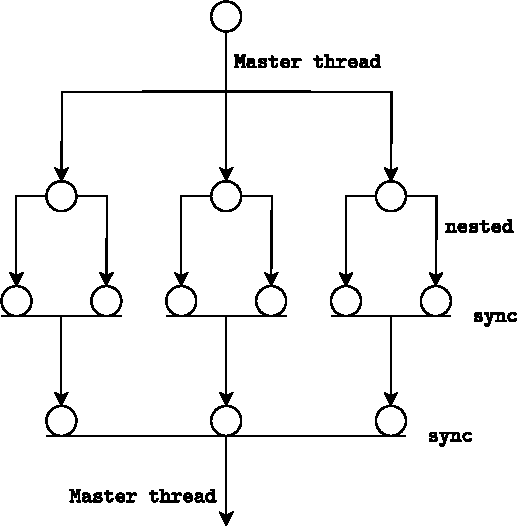
\includegraphics[width=.6\textwidth]{img/openmp-fork-join-1.pdf}
    \caption{OpenMP fork-join model.}
\end{figure}

\begin{flushleft}
    \textcolor{Green3}{\faIcon{question-circle} \textbf{What is the life history of each thread (\emph{slave}) created?}}
\end{flushleft}
All team members execute the code inside the \texttt{parallel} construct. When a thread finishes its work within the parallel construct, it waits at the implicit barrier at the end of the parallel construct. When all team members have arrived at the barrier, the threads can leave the barrier. The \emph{master} thread continues execution of user code beyond the end of the \texttt{parallel} construct, while the \emph{slave} threads wait to be summoned to join other teams.

\highspace
OpenMP \textbf{parallel regions can be nested inside each other}. If nested parallelism is:
\begin{itemize}
    \item \textbf{Disabled}, then the \textbf{new team} created by a thread encountering a parallel construct inside a parallel region \textbf{consists only of the encountering thread}.
    \item \textbf{Enabled}, then the \textbf{new team may consist of more than one thread}.
\end{itemize}

\newpage

\begin{flushleft}
    \textcolor{Green3}{\faIcon{box-open} \textbf{How does OpenMP manage the available threads? Thread Pool}}
\end{flushleft}
The OpenMP runtime library maintains a pool of threads that can be used as \emph{slave} threads in parallel regions. When a thread encounters a parallel construct and needs to create a team of more than one thread, the thread will check the pool and grab idle threads from the pool, making them \emph{slave} threads of the team. The \emph{master} thread might get fewer \emph{slave} threads than it needs if there is not a sufficient number of idle threads in the pool. When the team finishes executing the parallel region, the \emph{slave} threads return to the pool.

\highspace
\begin{flushleft}
    \textcolor{Red2}{\faIcon{bookmark} \textbf{Summary}}
\end{flushleft}
\begin{enumerate}
    \item \textbf{Parallel construct}. Our main thread starts to execute our code. It encounters a \texttt{parallel} construct.
    
    \item \textbf{Pool verification}. The OpenMP library checks its pool of threads. If within its pool of available threads have something of disposable, it allocates the \emph{slave} (thread requested) to the \emph{master} (thread that want to create the team). We refer to a single thread, but obviously this can be extended to multiple thread request (e.g. \emph{master} thread requests 3 threads to OpenMP). Finally, the number of requested \emph{slave}s cannot always be satisfied; OpenMP guarantees the best, so it continues to give the requested threads to the applicants. If it cannot satisfy the request, it returns the maximum number of \emph{slave}s it can satisfy (e.g. \emph{master} requests 4 threads, but OpenMP has a pool of only 2 threads available; therefore it returns 2 \emph{slave}s).
    
    \item \textbf{Assign and start execution}. Ideally, OpenMP returns the number of threads requested by the \emph{master}. Otherwise, it returns the maximum number. The team now consists of the main thread, called the \emph{master}, and its \emph{slave}s. Each member of the team executes the code specified by the programmer within the parallel construct.
    
    \item \textbf{End of execution of a thread}. A thread of the team finishes its work. It can finally rest, and its state changes from "running" to "waiting". It waits for its other thread friends. Each thread has an implicit barrier at the end of the parallel construct.
    
    \item \textbf{Any thread finish}. Finally, each thread finishes its work. The \emph{master} releases each member of the team to the OpenMP library. OpenMP updates its thread pool with the returning threads, and the \emph{master} thread continues its life independently from the released threads.
\end{enumerate}
The previous flow works if and only if nested parallelism is enabled. Otherwise, if a \emph{master} asks to create a new team, it will ignore the request and tell the requester to continue alone.

\newpage

\begin{flushleft}
    \textcolor{Green3}{\faIcon{tools} \textbf{Implementation}}
\end{flushleft}
Nested parallelism can be enabled or disabled by passing true or false as arguments to the runtime function:
\marginpar{
    \href{https://www.openmp.org/spec-html/5.0/openmpsu119.html\#x156-6930003.2.10} {Doc. \faIcon{book}}
}
\begin{openmpbox}[: \texttt{omp\_set\_nested}]
    \begin{lstlisting}[language=C++]
void omp_set_nested(int nested)\end{lstlisting}
\end{openmpbox}

\noindent
We can set a \textbf{default number of threads at different levels of nested parallelism} with:
\begin{center}
    \texttt{OMP\_NUM\_THREADS = [list, of, integers]}
\end{center}
If the nesting level is deeper than the number of entries in the list, the last value is used for all subsequent nested parallel region.

\begin{itemize}
    \item \texttt{OMP\_MAX\_ACTIVATE\_LEVELS} defines the upper \textbf{limit on the number of active parallel regions that may be nested}.

    \item \texttt{OMP\_THREAD\_LIMIT} \textbf{avoids} that recursive applications \textbf{create too many threads}.
\end{itemize}
Finally, since we are in nested parallelism, the thread number returns the thread number partially and not globally, we need other useful functions:
\begin{itemize}
    \item Returns the maximum number of OpenMP threads available in contention group:
    \marginpar{
        \href{https://www.openmp.org/spec-html/5.0/openmpsu123.html\#x160-7180003.2.14} {Doc. \faIcon{book}}
    }
    \begin{openmpbox}[: \texttt{omp\_get\_thread\_limit}]
        \begin{lstlisting}[language=C++]
int omp_get_thread_limit()\end{lstlisting}
    \end{openmpbox}

    \item Returns the maximum number of nested active parallel regions when the innermost parallel region is generated by the current task.
    \marginpar{
        \href{https://www.openmp.org/spec-html/5.0/openmpsu126.html\#x163-7370003.2.17} {Doc. \faIcon{book}}
    }
    \begin{openmpbox}[: \texttt{omp\_get\_max\_active\_levels}]
        \begin{lstlisting}[language=C++]
int omp_get_max_active_levels()\end{lstlisting}
    \end{openmpbox}
    
    \item Limits the number of nested active parallel regions when a new nested parallel region is generated by the current task.
    \marginpar{
        \href{https://www.openmp.org/spec-html/5.0/openmpsu125.html\#x162-7300003.2.16} {Doc. \faIcon{book}}
    }
    \begin{openmpbox}[: \texttt{omp\_set\_max\_active\_levels}]
        \begin{lstlisting}[language=C++]
void omp_set_max_active_levels(int $\emph{max\_levels}$)\end{lstlisting}
    \end{openmpbox}
    
    \newpage

    \item Returns the number of nested parallel regions on the device that enclose tha task containing the call.
    \marginpar{
        \href{https://www.openmp.org/spec-html/5.0/openmpsu127.html\#x164-7430003.2.18} {Doc. \faIcon{book}}
    }
    \begin{openmpbox}[: \texttt{omp\_get\_level}]
        \begin{lstlisting}[language=C++]
int omp_get_level()\end{lstlisting}
    \end{openmpbox}
    
    \item Returns the number of active, nested parallel regions on the device enclosing the task containing the call.
    \marginpar{
        \href{https://www.openmp.org/spec-html/5.0/openmpsu130.html\#x167-7610003.2.21} {Doc. \faIcon{book}}
    }
    \begin{openmpbox}[: \texttt{omp\_get\_active\_level}]
        \begin{lstlisting}[language=C++]
int omp_get_active_level()\end{lstlisting}
    \end{openmpbox}
    
    \item Returns, for given nested level of the current thread, the thread number of the ancestor of the current thread.
    \marginpar{
        \href{https://www.openmp.org/spec-html/5.0/openmpsu128.html\#x165-7490003.2.19} {Doc. \faIcon{book}}
    }
    \begin{openmpbox}[: \texttt{omp\_get\_ancestor\_thread\_num}]
        \begin{lstlisting}[language=C++]
int omp_get_ancestor_thread_num(int $\emph{level}$)\end{lstlisting}
    \end{openmpbox}
    
    \item Returns, for a given nested level of the current thread, the size of the thread team to which the ancestor of the current thread belongs.
    \marginpar{
        \href{https://www.openmp.org/spec-html/5.0/openmpsu129.html\#x166-7550003.2.20} {Doc. \faIcon{book}}
    }
    \begin{openmpbox}[: \texttt{omp\_get\_team\_size}]
        \begin{lstlisting}[language=C++]
int omp_get_team_size(int $\emph{level}$)\end{lstlisting}
    \end{openmpbox}
\end{itemize}
    \subsection{Cancellation}

As of OpenMP 4.0, a thread can be cancelled using a combination of two commands:
\begin{itemize}
    \item \texttt{cancel} construct cancels the innermost enclosing region of the specified type.
    
    In other words, it \textbf{allows us to cancel the current thread}. But be careful! The directive only allows to \textbf{set the cancellation flag to a value of one}. So it is necessary to also use the \texttt{cancellation point} command or the thread must hit a barrier (implicit or explicit).

    The syntax of the \texttt{cancel} construct is as follows:
    \marginpar{
        \href{https://www.openmp.org/spec-html/5.0/openmpsu101.html} {Doc. \faIcon{book}}
    }
    \begin{openmpbox}[: \texttt{pragma omp cancel}]
        \begin{lstlisting}[language=C++, mathescape=true]
#pragma omp cancel $\emph{construct-type-clause}$\end{lstlisting}
        Where \texttt{\emph{construct-type-clause}} is one of the following: \texttt{parallel}, \texttt{sections}, \texttt{for}, \texttt{taskgroup}.
    \end{openmpbox}
    
    \item The \texttt{cancellation point} construct introduces a user-defined cancellation\break point at which implicit or explicit tasks check whether cancellation of the innermost enclosing region of the specified type has been enabled.

    In other words, \textbf{when a thread encounters the cancellation point, the cancellation flag has been checked}. The thread execution is stopped. This is an explicit cancellation request because there are other points where cancellation flag is checked, such as at another cancel region or at a barrier.
    \marginpar{
        \href{https://www.openmp.org/spec-html/5.0/openmpsu102.html\#x134-5350002.18.2} {Doc. \faIcon{book}}
    }
    \begin{openmpbox}[: \texttt{pragma omp cancellation point}]
        \begin{lstlisting}[language=C++]
#pragma omp cancellation point\end{lstlisting}
    \end{openmpbox}
\end{itemize}
Since there is an \textbf{overhead in checking for cancellation}, it can be enabled manually using the \texttt{OMP\_CANCELLATION} environment variable (false by default).

\begin{flushleft}
    \textcolor{Red2}{\faIcon{exclamation-triangle} \textbf{Immediate cancellation is not guaranteed}}
\end{flushleft}
\textbf{OpenMP does not guarantee that cancellation will result in immediate termination}.

\highspace
\begin{flushleft}
    \textcolor{Green3}{\faIcon{check} \textbf{When to use?}}
\end{flushleft}
When there is a \textbf{need to stop the execution}, such as in the \textbf{divide-and-conquer algorithms} (for example, to stop a search when we find the element), or when we \textbf{need to handle some errors}.

\begin{examplebox}[: thread cancellation]
    Assume that from a certain point in our algorithm there are 5 threads alive (including the \emph{master}), and the construct pipeline is as follows.
    \begin{center}
        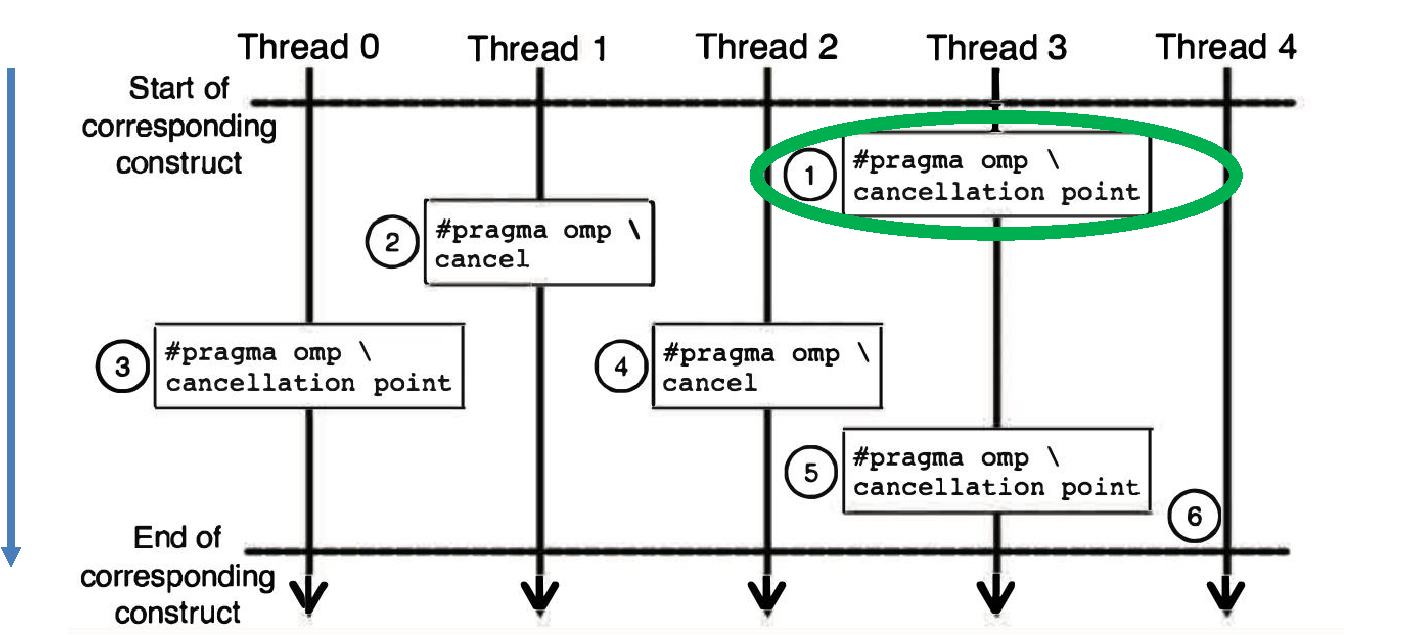
\includegraphics[width=\textwidth]{img/openmp-cancel-1.pdf}
    \end{center}

    Thread 3 hits a cancellation point, but there is no cancel directive before it, so the cancellation flag is set to zero by default and the thread hasn't been broken.
    \begin{center}
        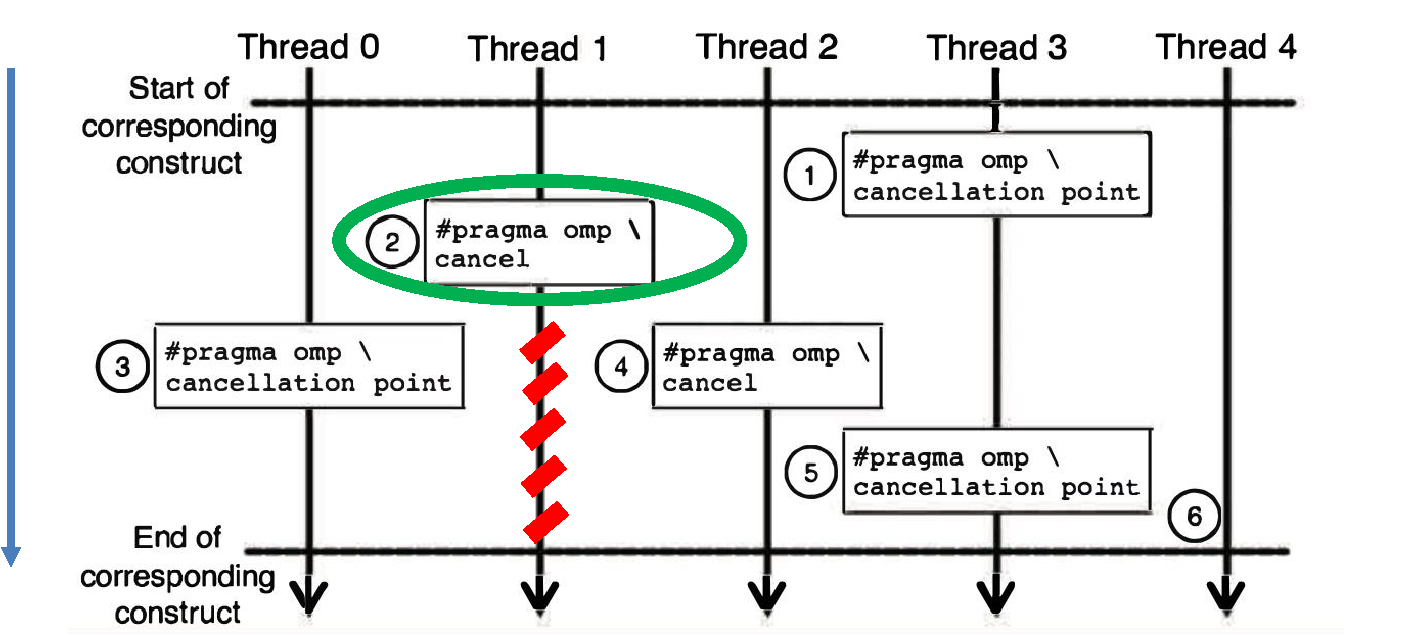
\includegraphics[width=\textwidth]{img/openmp-cancel-2.pdf}
    \end{center}

    Thread 1 requests the cancellation and waits for a synchronization point, such as a barrier or an cancellation point. From that point on, it is idle and waits.
    \begin{center}
        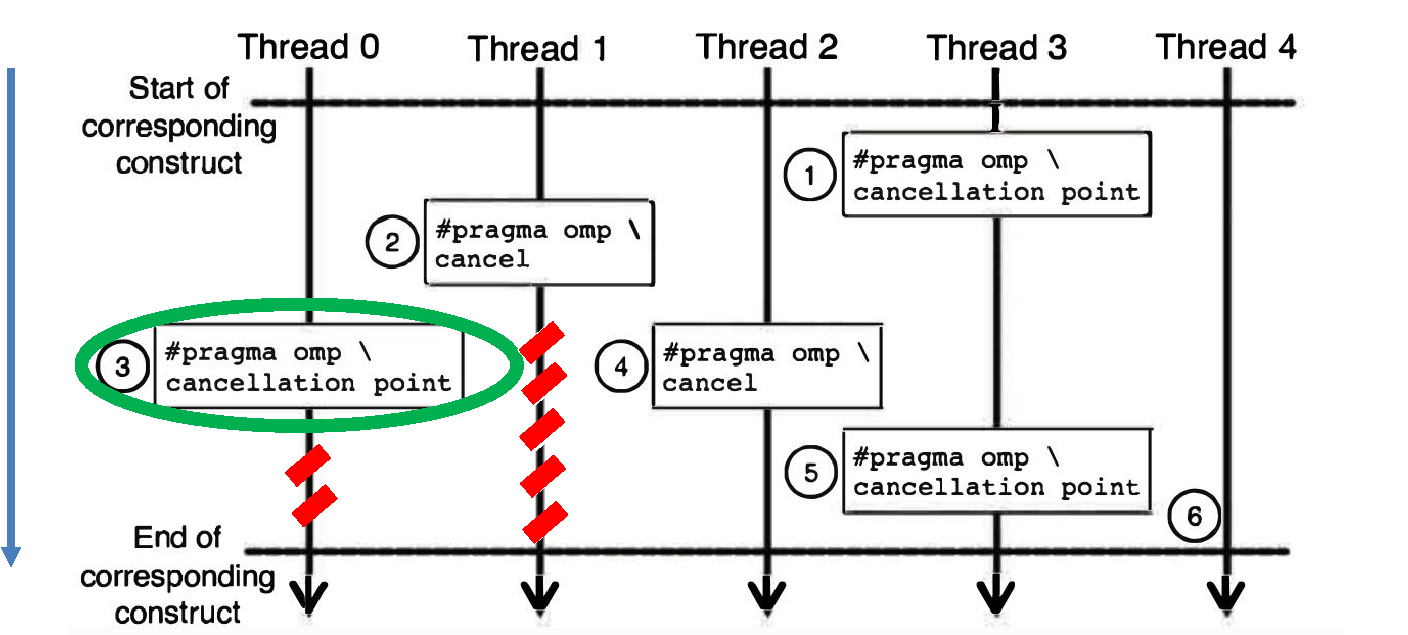
\includegraphics[width=\textwidth]{img/openmp-cancel-3.pdf}
    \end{center}

    Thread 0 calls a cancellation point to check the flag and terminates because thread 1 (last step) has set the cancellation flag to 1. At this point, thread 1, which was waiting for a synchronization point, also terminates.
    \begin{center}
        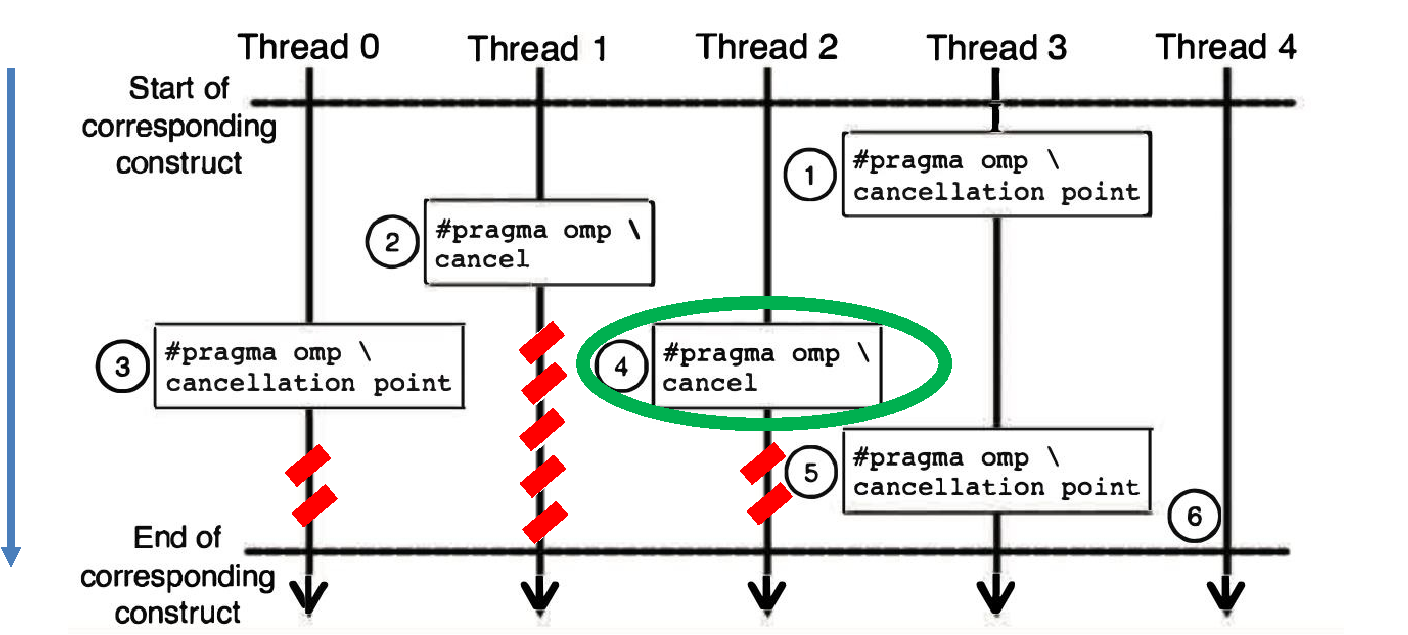
\includegraphics[width=\textwidth]{img/openmp-cancel-4.pdf}
    \end{center}
    
    At the same time, thread 2 is cancelled because the cancel directive checks the cancellation flag first.
    \begin{center}
        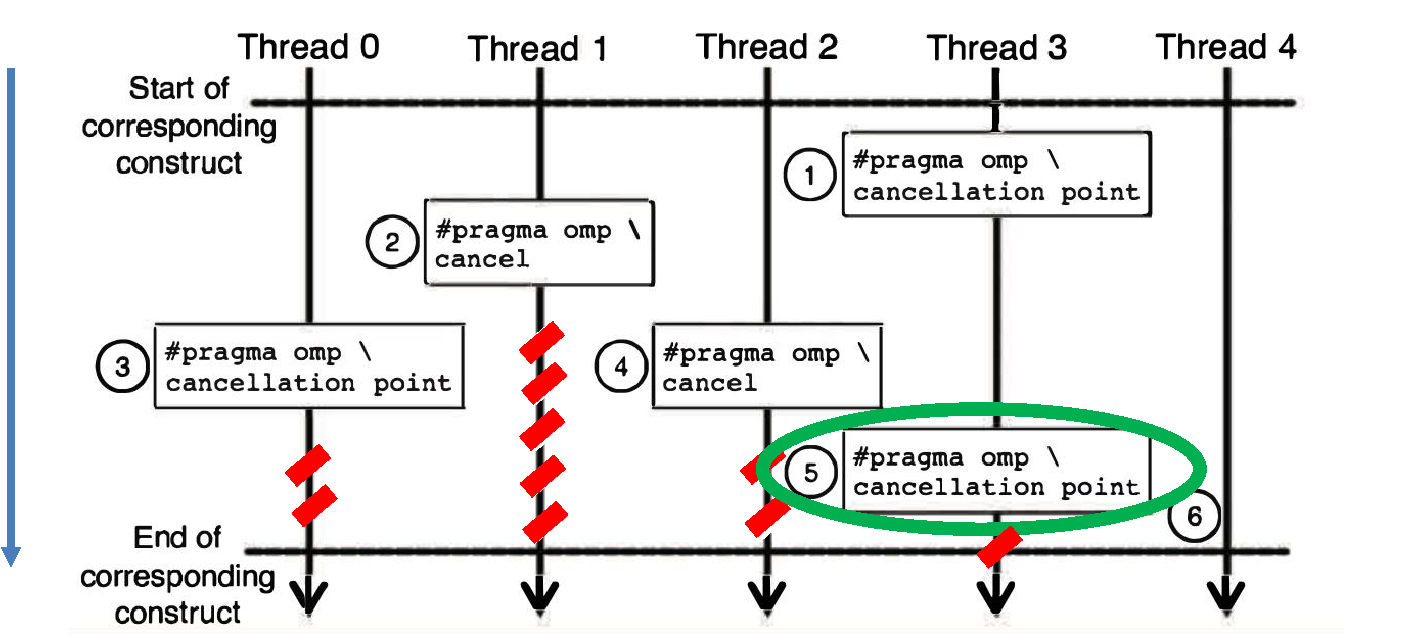
\includegraphics[width=\textwidth]{img/openmp-cancel-5.pdf}
    \end{center}

    At this point the thread 3 has been terminated.
    \begin{center}
        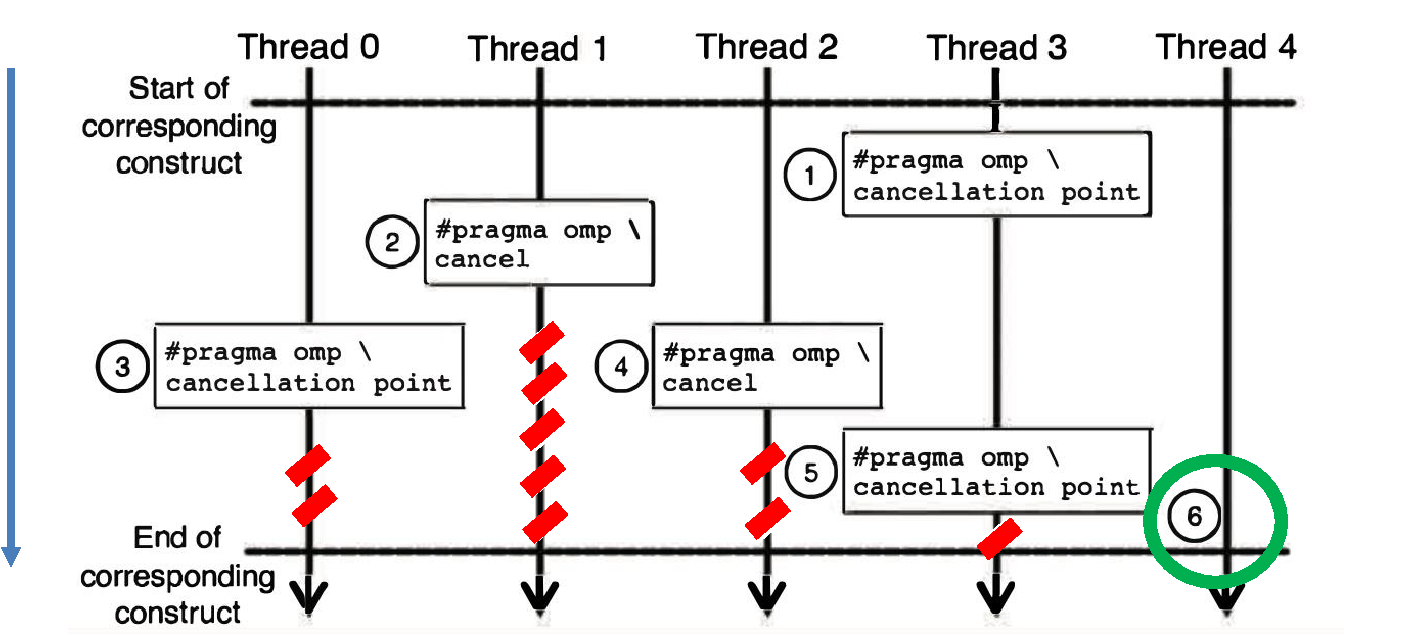
\includegraphics[width=\textwidth]{img/openmp-cancel-6.pdf}
    \end{center}

    Finally, thread 4 never encounters a cancellation point and finishes execution normally.
\end{examplebox}
    \subsection{SIMD Vectorization}

A \textbf{SIMD processor exploits data parallelism by providing instructions that operate on blocks of data} (called \textbf{vectors}). SIMD provides \textbf{data parallelism at the instruction level} and can be combined with other OpenMP constructs to achieve multi-level parallelism.

\highspace
\begin{flushleft}
    \textcolor{Red2}{\faIcon{times-circle} \textbf{What compilers must do to understand whether a loop can be vectorized}}
\end{flushleft}
SIMD instructions use \textbf{SIMD registers}. The compilers deal with \textbf{several issues to determine whether a loop can be vectorized by SIMD instructions}. It does:
\begin{itemize}
    \item An analysis of the dependencies across iterations;
    \item An alias analysis of pointers;
    \item An analysis of the data layout/alignment issues;
    \item An analysis of conditional executions;
    \item Checks of the loop bounds that must not be multiple of vector length.
\end{itemize}

\highspace
\begin{flushleft}
    \textcolor{Red2}{\faIcon{times-circle} \textbf{Other compiler problems: Loop Peeling and Loop Tail}}
\end{flushleft}
Also, the \textbf{loop iterations at the beginning and end may not be vectorized} (loop peeling, tail). This is because when a compiler tries to optimize a loop using vectorization (i.e., applying the same operation to multiple data points simultaneously to speed up execution), it often encounters problems with the iterations at the beginning and end of the loop. These iterations may not fit neatly into the vectorized operations because the total number of iterations of the loop may not be a perfect multiple of the vector length.

\highspace
Essentially, the \textbf{compiler may have to split the loop into three parts}:
\begin{enumerate}
    \item \definition{Loop Peeling}. Handle the initial few iterations that don't align with vector boundaries.

    \item \textbf{Vectorized Main Loop}. Process the majority of the loop iterations using vectorized operations.

    \item \definition{Loop Tail}. Handle the remaining iterations that can't be processed with vector operations due to their small number.
\end{enumerate}
This approach ensures that the loop is as optimized as possible, even if some parts of it cannot be vectorized efficiently.

\newpage

\begin{flushleft}
    \textcolor{Green3}{\faIcon{tools} \textbf{Use OpenMP SIMD}}
\end{flushleft}
The \texttt{simd} construct can be applied to a loop to indicate that the loop can be transformed into a SIMD loop (i.e., multiple iterations of the loop can be executed simultaneously using SIMD instructions).

\marginpar{
    \href{https://www.openmp.org/spec-html/5.0/openmpsu42.html\#x65-1390002.9.3} {Doc. \faIcon{book}}
}
\begin{openmpbox}[: \texttt{pragma omp simd}]
    \begin{lstlisting}[language=C++]
#pragma omp simd\end{lstlisting}
\end{openmpbox}

\noindent
The \textbf{loop is divided into chunks}, and \textbf{all iterations are executed by a single thread using SIMD vector instructions}. The \textbf{chunks should fit into a vector register} for \textcolor{Green4}{\textbf{performance}}, and \textbf{each iteration is executed by a \emph{SIMD lane}}. The compiler will generate SIMD instructions, it is \textbf{up to the user to ensure this maintains correct behavior}.

\highspace
\begin{flushleft}
    \textcolor{Green3}{\faIcon{question-circle} \textbf{Possible clauses}}
\end{flushleft}
\begin{itemize}
    \item Data scope clauses (page \pageref{subsection: Data environment}) can be used in a \texttt{simd} directive.

    \item A \texttt{collapse} clause can be \textbf{used to fuse two perfectly nested loops, but the complexity can be increase}.
    
    \item The \texttt{simdlen(\emph{size})} clause suggests a \textbf{preferred vector length}. Maybe the code will work better with a specific vector length, but the compiler is free to ignore it (is only a suggestion make by the programmer). It can also hurt performance but the results remain correct.
    
    \item The \texttt{safelen(\emph{size})} clause sets an \textbf{upper limit to the vector length that the compiler cannot exceed}.
\end{itemize}

\highspace
\begin{flushleft}
    \textcolor{Green3}{\faIcon{tachometer-alt} \textbf{For SIMD}}
\end{flushleft}
The \texttt{omp for simd} directive \textbf{distributes the iterations of one or more associated loops across the threads} that already exist in the team \textbf{and indicates that the iterations executed by each thread can be executed concurrently using SIMD instructions}.

\begin{openmpbox}[: \texttt{pragma omp for simd}]
    \begin{lstlisting}[language=C++]
#pragma omp for simd\end{lstlisting}
\end{openmpbox}

\noindent
The \textbf{number of threads and scheduling policy greatly affect performance}. If the \textbf{number of threads increases, work for each thread is smaller}. \textbf{Each thread should work with a chunk corresponding to the vector length}. Ideally, it is correct to distribute iterations among threads in a team, then each thread uses SIMD instructions.

\newpage

\noindent
The clause \texttt{schedule} \textbf{avoid performance degradation specifying the scheduling type and chunk size for the loop iterations}. The \texttt{static} schedule divides the iterations into chunks of \texttt{\emph{chunk-size}}, distributing them to the threads.
\begin{openmpbox}[: \texttt{pragma omp declare simd}]
    \begin{lstlisting}[language=C++, mathescape=true]
#pragma omp for simd schedule(simd:static, $\emph{chunk-size}$)\end{lstlisting}
\end{openmpbox}

\highspace
Finally, we can also \textbf{declare a function to be compiled for calls inside a SIMD loop}.
\begin{openmpbox}[: \texttt{pragma omp declare simd}]
    \begin{lstlisting}[language=C++]
#pragma omp declare simd
    /* function definition */\end{lstlisting}
\end{openmpbox}

    %%%%%%%%%%%%%%%%%%%%
    % GPU Architecture %
    %%%%%%%%%%%%%%%%%%%%
    \section{CUDA}

\subsection{Introduction}

\definition{CUDA}, which stands for \textbf{Compute Unified Device Architecture}, is a \textbf{parallel computing platform and application programming interface (API) model created by NVIDIA}. It allows developers to use the power of GPUs (Graphics Processing Units) for general-purpose processing, which enables substantial performance improvements for computationally intensive tasks.

\highspace
\begin{flushleft}
    \textcolor{Green3}{\faIcon{question-circle} \textbf{Why CUDA?}}
\end{flushleft}
GPUs, originally designed to render graphics, have evolved into \textbf{highly efficient and powerful processors capable of handling thousands of threads simultaneously}. This transformation has made GPUs, and by extension CUDA, incredibly valuable for applications requiring massive parallelism, such as scientific simulations, machine learning, and deep learning.

\highspace
\begin{flushleft}
    \textcolor{Green3}{\faIcon{question-circle} \textbf{Why can we not just use the CPU?}}
\end{flushleft}
Understanding the fundamental differences between CPU and GPU architectures is key to appreciating CUDA's advantages:
\begin{itemize}
    \item CPU (Central Processing Unit):
    \begin{itemize}
        \item Designed for sequential processing.
        \item Features powerful Arithmetic Logic Units (ALUs) with low latency.
        \item Utilizes large hierarchical caches to optimize access to frequently used data.
        \item Employs advanced control mechanisms, such as branch prediction and data forwarding, to minimize delays.
    \end{itemize}

    \item GPU (Graphics Processing Unit):
    \begin{itemize}
        \item Optimized for parallel processing.
        \item Contains a large number of simpler, pipelined ALUs designed for high-throughput computations, despite having longer latency.
        \item Relies on smaller caches to facilitate high memory throughput.
        \item Uses simpler control mechanisms, enabling efficient context switching and handling many threads concurrently.
    \end{itemize}
\end{itemize}
CUDA leverages these GPU characteristics to execute programs with a parallel-first approach, breaking down tasks into smaller, manageable pieces and processing them simultaneously. This approach leads to significant speedups compared to traditional CPU-only processing, making CUDA a pivotal technology for high-performance computing.

    \subsection{GPU compute mode}

\definition{GPU compute mode} refers to \textbf{GPU hardware that is optimized for general-purpose computing rather than graphics rendering}. This mode allows users to run non-graphics programs on the GPU's programmable cores, taking advantage of the GPU's parallel processing capabilities for tasks such as scientific simulations, data analysis, and machine learning.

\begin{examplebox}[: how to run code on a GPU (prior to 2007)]
    Now let us see how to run a simple code on a GPU. Suppose a user wants to draw a picture on a GPU:
    \begin{itemize}
        \item \textbf{GPU Shader Program Binaries}. The application, via the graphics driver, supplies the GPU with shader program binaries. These are compiled programs that the GPU will execute to perform rendering tasks.
        
        \item \textbf{Graphics Pipeline Parameters}. The application sets various parameters for the graphics pipeline, such as the output image size, to control how the rendering should be processed.
        
        \item \textbf{Vertex Buffer}. The application provides the GPU with a buffer of vertices. Vertices are data points that define the shape of the objects to be rendered.
        
        \item \textbf{Draw Command}. The application sends a draw command to the GPU using the function call \texttt{drawPrimitives(vertex\_buffer)}. This command instructs the GPU to start rendering using the provided vertex data.
    \end{itemize}
    The stages of the graphics pipeline:
    \begin{enumerate}
        \item \textbf{Input Vertex Buffer}: The initial stage where the vertex data is input to the pipeline.

        \item \textbf{Vertex Generation}: Vertices are generated or fetched from the vertex buffer.
        
        \item \textbf{Vertex Processing}: The vertices undergo various transformations and shading calculations.
        
        \item \textbf{Primitive Generation}: The processed vertices are used to generate geometric primitives (such as triangles).
        
        \item \textbf{Fragment Generation (Rasterization)}: The primitives are converted into fragments (potential pixels).
        
        \item \textbf{Fragment Processing}: Fragments undergo shading and texturing calculations to determine their final color and properties.
        
        \item \textbf{Pixel Operations}: Final operations are performed on the fragments, such as depth testing and blending.
        
        \item \textbf{Output Image Buffer}: The processed fragments are written to the output image buffer, resulting in the final rendered image.
    \end{enumerate}
\end{examplebox}

\begin{flushleft}
    \textcolor{Green3}{\faIcon{history} \textbf{Some history}}
\end{flushleft}
\textbf{Before 2007} the \textbf{only way to interface with GPU hardware was through the graphics pipeline}. This meant that GPUs were \emph{\textbf{designed and used specifically for tasks related to graphics rendering}}. The pipeline stages (such as vertex processing, fragment generation, and pixel operations) were all designed to transform vertex data into pixels displayed on the screen.

\highspace
Because they were optimized to handle parallel tasks associated with rendering images, their architecture and interfaces were tightly coupled with graphics APIs.

\highspace
\textbf{By 2007}, the concept of using GPUs for \definition{General-Purpose computing on Graphics Processing Units (GPGPU)} was emerging. Thanks mainly to the introduction of a new architecture signed NVIDIA called Tesla and CUDA, a parallel computing platform and programming model (also OpenCL was emerging).

\highspace
The \definition{NVIDIA Tesla architecture}, introduced with the \href{https://www.techpowerup.com/gpu-specs/geforce-8800-gt.c201}{GeForce 8800 GPU} in 2006, marked a significant shift in GPU design by unifying graphics and computing capabilities. This architecture featured a scalable parallel array of processors that could be programmed in \texttt{C} or via graphics \texttt{APIs2}. The Tesla architecture enabled \textbf{flexible}, \textbf{programmable graphics and high-performance computing}, making it possible to use GPUs for a wide range of applications beyond traditional graphics rendering. This unification enabled massive multithreading and parallel processing, dramatically improving performance for computationally intensive tasks.\cite{lindholm2008nvidia}

\highspace
From this point on, the programmable cores of the GPU are used:
\begin{itemize}
    \item Application could allocate buffers in GPU memory and copy data to/from buffers;
    \item Application (via the graphics driver) provides a single kernel program binary to the GPU;
    \item Application tells GPU to run kernel in SPMD fashion.
\end{itemize}
    \subsection{CUDA}

\subsubsection{Basics of CUDA}

\begin{flushleft}
    \textcolor{Green3}{\faIcon{question-circle} \textbf{What is CUDA?}}
\end{flushleft}
\definition{Compute Unified Device Architecture (CUDA)}, is a \textbf{parallel computing platform and Application Programming Interface} (API) \textbf{model} created by NVIDIA. It allows developers to utilize NVIDIA GPUs for general-purpose processing, enabling them to perform a wide range of computations more efficiently than with traditional CPU processing alone.

\highspace
CUDA was introduced with the NVIDIA Tesla architecture, which marked a significant shift in GPU capabilities, enabling general purpose computing on GPUs. \textbf{CUDA is designed to be similar to the \texttt{C} programming language}, making it familiar to many developers. It allows programmers to write code that runs on GPUs using the compute-mode hardware interface.

\highspace
\textbf{CUDA's abstractions are relatively low-level and closely match the performance characteristics and capabilities of modern GPUs}. This design goal helps maintain a low abstraction layer, ensuring that developers can take full advantage of the hardware's potential.

\highspace
Note that \definition{Open Computing Language (OpenCL)} is an open standards version of CUDA that runs on both CPUs and GPUs from multiple vendors. \textbf{While CUDA runs only on NVIDIA GPUs, OpenCL is designed to be more versatile and work on hardware from multiple vendors}.

\highspace
\begin{flushleft}
    \textcolor{Green3}{\faIcon{question-circle} \textbf{CUDA Thread Hierarchy}}
\end{flushleft}
CUDA organizes threads into a hierarchical structure to efficiently manage parallel computations on GPUs. To understand how it works, let's look at it from the deepest level up:
\begin{enumerate}
    \item \textbf{Threads}. Threads (or \definition{CUDA Threads}) are the \textbf{smallest unit of execution} in CUDA. Each thread runs a single instance of a kernel function\footnote{A kernel function in CUDA is a function that runs on the GPU (device) but is called from the CPU (host). These functions are executed by many parallel threads on the GPU}.
    
    Threads are \textbf{identified by their unique thread IDs}, which are used to calculate memory addresses and control decisions.
    

    \item \textbf{Thread Blocks}. Threads are grouped into blocks (called also \definition{CUDA Blocks}). Each block can contain multiple threads that execute concurrently.
    
    \textbf{Threads within the same block can communicate and share data} through shared memory and synchronization primitives like barriers and atomic operations.
    
    The \emph{maximum number} of threads per block is limited by the GPU architecture, typically up to 1024 threads per block.
    
    \label{definition: CUDA Grids}
    \item \textbf{Grids}. Blocks are organized into a grid (called also \definition{CUDA Grids}). A grid is a \textbf{collection of blocks that execute the same kernel function}.
    
    All \textbf{threads in a grid share the same global memory space}.
    
    The grid can be multi-dimensional, allowing for flexible organization of blocks to match the problem's dimensions.
\end{enumerate}
Note that CUDA uses the \texttt{x}, \texttt{y}, and \texttt{z} dimensions for threads, blocks, and grids because this \textbf{multi-dimensional structure} aligns well with many common computational problems. Many computational problems naturally fit into a multi-dimensional space. For example, image processing involves 2D data, and volumetric simulations involve 3D data.

\begin{figure}[!htp]
    \centering
    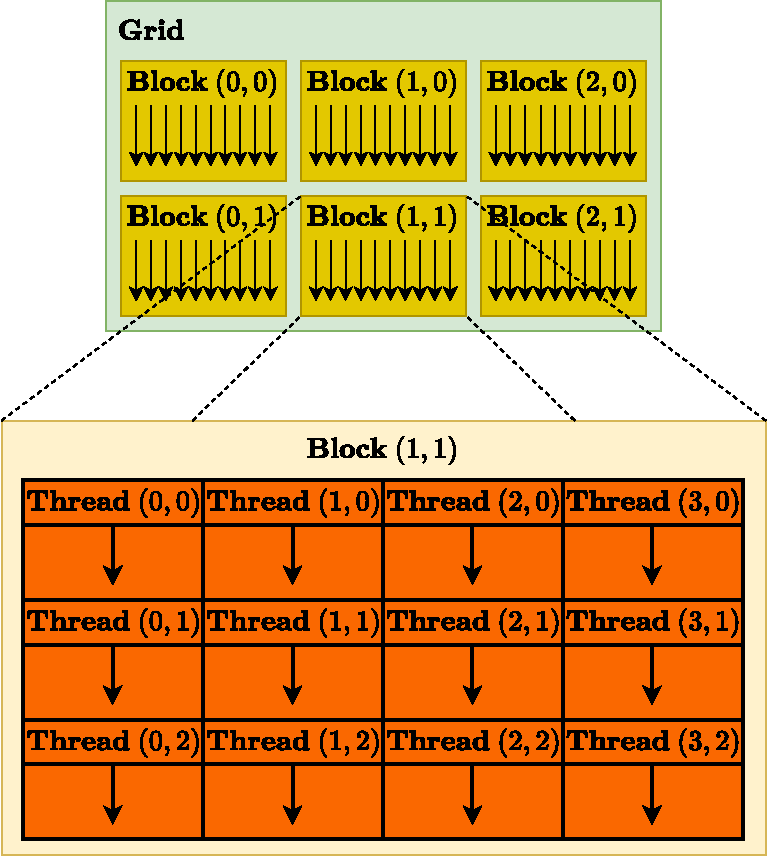
\includegraphics[width=.8\textwidth]{img/CUDA-blocks-grid-threads-1.pdf}
    \caption{The figure shows an example of a CUDA grid consisting of 6 blocks, each block consisting of 12 threads. The number of threads and the number of blocks per column/row are customizable, this is just an example. In total, there are 72 CUDA threads (12 threads per block times 6 blocks in the grid).}
    \label{fig: CUDA example of Grid, Blocks and Threads}
\end{figure}

\begin{flushleft}
    \textcolor{Green3}{\faIcon{calculator} \textbf{CUDA Kernels}}
\end{flushleft}
A \definition{CUDA kernel} is a \textbf{function that gets executed on the GPU}. It contains the parallel portion of the application, which is executed by multiple threads in parallel. Unlike regular C/C++ functions that run on a single thread, CUDA kernels can run thousands of threads simultaneously.

\newpage

\begin{flushleft}
    \textcolor{Green3}{\faIcon{balance-scale} \textbf{Device vs Host}}
\end{flushleft}
In CUDA, there is a term to identify the code that runs on the CPU and GPU.
\begin{definitionbox}[: CUDA Host (CPU)]
    The \definition{CUDA Host} \textbf{refers to the CPU} and its associated memory.

    It is \textbf{responsible for managing the overall program execution}. This includes allocating memory, launching CUDA kernels, and transferring data between the CPU and the GPU.

    It is typically written in the standard programming language used (e.g., C, C++, Java, Python, etc.) and contains the logic for setting up and controlling the execution of CUDA kernels on the device.
\end{definitionbox}

\begin{definitionbox}[: CUDA Device (GPU)]
    The \definition{CUDA Device} \textbf{refers to the GPU} and its associated memory.

    It is \textbf{responsible for running parallel code} (CUDA kernels) and \textbf{performs the bulk of the computation}. This takes advantage of the parallel processing power of the GPU.
    
    The device code (kernels) is written in the CUDA programming language and is designed to run on the multiple parallel cores of the GPU.
\end{definitionbox}

\begin{flushleft}
    \textcolor{Green3}{\faIcon{code} \textbf{Basic CUDA syntax}}
\end{flushleft}
Here is a sample code written in CUDA:
\begin{lstlisting}[language=C++]
#include <cuda_runtime.h>
#include <iostream>
#define Nx 12   $\label{code: CUDA basic - const def 1}$
#define Ny 6    $\label{code: CUDA basic - const def 2}$

// Kernel definition
__global__ void MatAdd( $\label{code: CUDA basic - MatAdd}$
    float A[Ny][Nx], 
    float B[Ny][Nx], 
    float C[Ny][Nx]
) {
    int i = blockIdx.x * blockDim.x + threadIdx.x;$\label{code: CUDA basic - index i}$
    int j = blockIdx.y * blockDim.y + threadIdx.y;$\label{code: CUDA basic - index j}$
    // guard against out of bounds array access
    if (i < N && j < N)                 $\label{code: CUDA basic - if condition}$
        C[i][j] = A[i][j] + B[i][j];    $\label{code: CUDA basic - sum}$
}

int main() {
    // Define the hierarchy
    dim3 threadsPerBlock(4, 3); $\label{code: CUDA basic - threadsPerBlock}$
    dim3 numBlocks(             $\label{code: CUDA basic - numBlocks}$
        Nx / threadsPerBlock.x, 
        Ny / threadsPerBlock.y
    );
    // Kernel invocation
    // Assume matrices A, B, C are already allocated (dim Nx x Ny)
    MatAdd<<<numBlocks, threadsPerBlock>>>(A, B, C); $\label{code: CUDA basic - MatAdd invocation}$
}
\end{lstlisting}
\begin{itemize}
    \item[Rows \ref{code: CUDA basic - const def 1}-\ref{code: CUDA basic - const def 2}] Variables \texttt{Nx} and \texttt{Ny} define the dimensions of the matrices. In this case, they are $12 \times 6$.
    
    \item[Row \ref{code: CUDA basic - threadsPerBlock}] The \texttt{threadsPerBlock} function specifies that each block will have 4\break threads in the \emph{x} dimension and 3 threads in the \emph{y} dimension. In other words, it defines how a block should be composed (see the figure \ref{fig: CUDA example of Grid, Blocks and Threads}).

    \item[Row \ref{code: CUDA basic - numBlocks}] The \texttt{numBlocks} function defines the number of blocks required to cover the entire matrix. The number of blocks is calculated by dividing the matrix dimensions by the number of threads per block in each dimension. In other words, it defines how a grid should be composed (see the figure \ref{fig: CUDA example of Grid, Blocks and Threads}).

    \item[Row \ref{code: CUDA basic - MatAdd invocation}] The execution configuration syntax \texttt{<}\texttt{<}\texttt{<}\texttt{...}\texttt{>}\texttt{>}\texttt{>} is required to specify the number of threads per block and the number of blocks per grid (both numbers can be of type \texttt{int} or \texttt{dim3}).
    
    The function invocation starts the \texttt{MatAdd} kernel with the given grid and block dimensions. This kernel runs on the GPU and performs the matrix addition.

    \item[Row \ref{code: CUDA basic - MatAdd}] Defines a kernel function called \texttt{MatAdd} to be executed on the GPU. The \texttt{\_\_global\_\_} keyword indicates that this is a kernel function.
    
    \item[Rows \ref{code: CUDA basic - index i}-\ref{code: CUDA basic - index j}] Computes the global column index i for each thread. This combines the block index and the thread index within the block to get the overall position.
    
    It also does the same with the j index.

    \item[Row \ref{code: CUDA basic - if condition}] The \texttt{if} condition ensures that the thread does not access out-of-bounds elements in the matrices.
    
    \item[Row \ref{code: CUDA basic - sum}] Finally, it performs the element-wise addition of matrices \texttt{A} and \texttt{B} and stores the result in matrix \texttt{C}.
\end{itemize}
As we said in Figure \ref{fig: CUDA example of Grid, Blocks and Threads} (page \pageref{fig: CUDA example of Grid, Blocks and Threads}), the example spawns 72 CUDA threads.
    \subsubsection{Memory model}\label{subsubsection: Memory model}

The CUDA memory model consists of several types of memory, each with different characteristics and uses. In general, the \textbf{Host (CPU) and the Device (GPU) have different address spaces}, each one has its private memory address.

\highspace
For example, the \texttt{cudaMemcpy} function in CUDA is used to \textbf{copy data} between different memory spaces, specifically \textbf{between host (CPU)} memory \textbf{and device (GPU) memory}.

\begin{lstlisting}[language=C++]
// allocate buffer in host mem
float* A = new float[N];

// populate host address space pointer A
for (int i = 0; i < N; ++i) {
    A[i] = (float)i;
}

// allocate buffer in device (GPU) address space
int bytes = sizeof(float) * N;
float* deviceA;
cudaMalloc(&deviceA, bytes);

// populate deviceA
cudaMemcpy(deviceA, A, bytes, cudaMemcpyHostToDevice);
// deviceA:
//      Destination memory address (either on the host or device).
//
// A:
//      Source memory address (either on the host or device).
//
// bytes:
//      Number of bytes to copy.
//
// cudaMemcpyHostToDevice:
//      Type of memory copy operation.
//      Copies data from host memory to device memory.
\end{lstlisting}
Note that directly accessing \texttt{deviceA[i]} is an invalid operation, because we cannot manipulate the contents of \texttt{deviceA} directly from host, since \texttt{deviceA} is not a pointer to the host's address space.

\newpage

\begin{flushleft}
    \label{CUDA memory: Types of CUDA device memory models visible to kernels}
    \textcolor{Green3}{\faIcon{memory} \textbf{Types of CUDA device memory models visible to kernels}}
\end{flushleft}
\begin{enumerate}
    \item \definition{Per-thread Private Memory}. This memory is \textbf{private to each}\break \textbf{thread}. Each thread has its own memory space that other threads cannot access.
    
    \textcolor{Green3}{\faIcon{question-circle} \textbf{Usage.}} It is \textbf{ideal for storing variables that are only relevant to individual threads} and do not need to be shared with other threads.
    
    \textcolor{Green3}{\faIcon{tachometer-alt} \textbf{Access.}} It has \textbf{fast access}, limited by the number of registers available.


    \item \definition{Per-block Shared Memory}. This memory is \textbf{shared by all threads within a block}. It allows threads within the same block to cooperate by sharing data.
    
    \textcolor{Green3}{\faIcon{question-circle} \textbf{Usage.}} It is useful for tasks where \textbf{threads within a block need to communicate or share intermediate results}. It is often used to optimize memory access patterns and reduce global memory accesses.
    
    \textcolor{Green3}{\faIcon{tachometer-alt} \textbf{Access.}} It is \textbf{much faster than global memory, but limited in size}. Access is almost as fast as registers when used properly.


    \item \definition{Device Global Memory}. This memory is \textbf{accessible to all threads across all blocks}. It provides a large amount of memory, but has higher latency and lower bandwidth than shared memory.
    
    \textcolor{Green3}{\faIcon{question-circle} \textbf{Usage.}} It is \textbf{suitable} for storing large amounts of \textbf{data that must be accessed by threads in different blocks}.
    
    \textcolor{Green3}{\faIcon{tachometer-alt} \textbf{Access.}} It has the \textbf{slowest access} of the three types, but is necessary for large data storage and inter-block communication.
\end{enumerate}
    \subsubsection{NVIDIA V100 Streaming Multiprocessor (SM)}

The NVIDIA V100 is a powerful GPU designed for data centers, primarily used for Artificial Intelligence (AI), High Performance Computing (HPC), and data science. Meanwhile, the \definition{NVIDIA V100 Streaming Multiprocessor (SM)} is a key component of the V100 GPU architecture.

\highspace
\begin{flushleft}
    \textcolor{Green3}{\faIcon{question-circle} \textbf{How is architecture composed?}}
\end{flushleft}
\begin{itemize}
    \item \textbf{Warp Selector and Fetch/Decode}:
    
    The \emph{Warp Selector} and \emph{Fetch/Decode} units are responsible for \textbf{managing the execution of warps} (groups of threads) and \textbf{decoding instructions}.


    \item \textbf{Functional Units}:
    \begin{itemize}
        \item \definitionWithSpecificIndex{SIMD fp32 functional unit}{NVIDIA V100 SM SIMD fp32 functional unit}{} (Yellow).
        
        It \textbf{handles single-precision floating-point operations}. Control is shared across 16 units, allowing for 16 multiply-add (\texttt{MUL-ADD}) operations per clock cycle. This translates to one 32-wide SIMD operation every two clocks.


        \item \definitionWithSpecificIndex{SIMD int functional unit}{NVIDIA V100 SM SIMD int functional unit}{} (Orange). 
        
        It \textbf{manages integer operations}, also shared across 16 units, with the same performance characteristics as the fp32 unit (16 $\times$ \texttt{MUL-ADD} per clock).
        

        \item \definitionWithSpecificIndex{SIMD fp64 functional unit}{NVIDIA V100 SM SIMD fp64 functional unit}{} (Brown). 
        
        It is \textbf{responsible for double-precision floating-point operations}. Control is shared across 8 units, allowing for 8 \texttt{MUL-ADD} operations per clock cycle, equating to one 32-wide SIMD operation every four clocks.
        

        \item \definitionWithSpecificIndex{Tensor core unit}{NVIDIA V100 SM Tensor core unit}{} (Red). 
        
        It is \textbf{specialized for tensor operations}, which are crucial for deep learning and AI workloads.
        

        \item \definitionWithSpecificIndex{Load/store unit}{NVIDIA V100 SM Load/store unit}{} (Green). 
        
        It \textbf{handles memory operations}, such as loading data from and storing data to memory.
    \end{itemize}


    \item \textbf{Warp Scheduler}:

    The diagram below shows the scheduling of warps (Warp 0, Warp 4, Warp 60, etc.) across the functional units, indicating how different warps are processed in parallel.
\end{itemize}

\newpage

\begin{figure}[!htp]
    \centering
    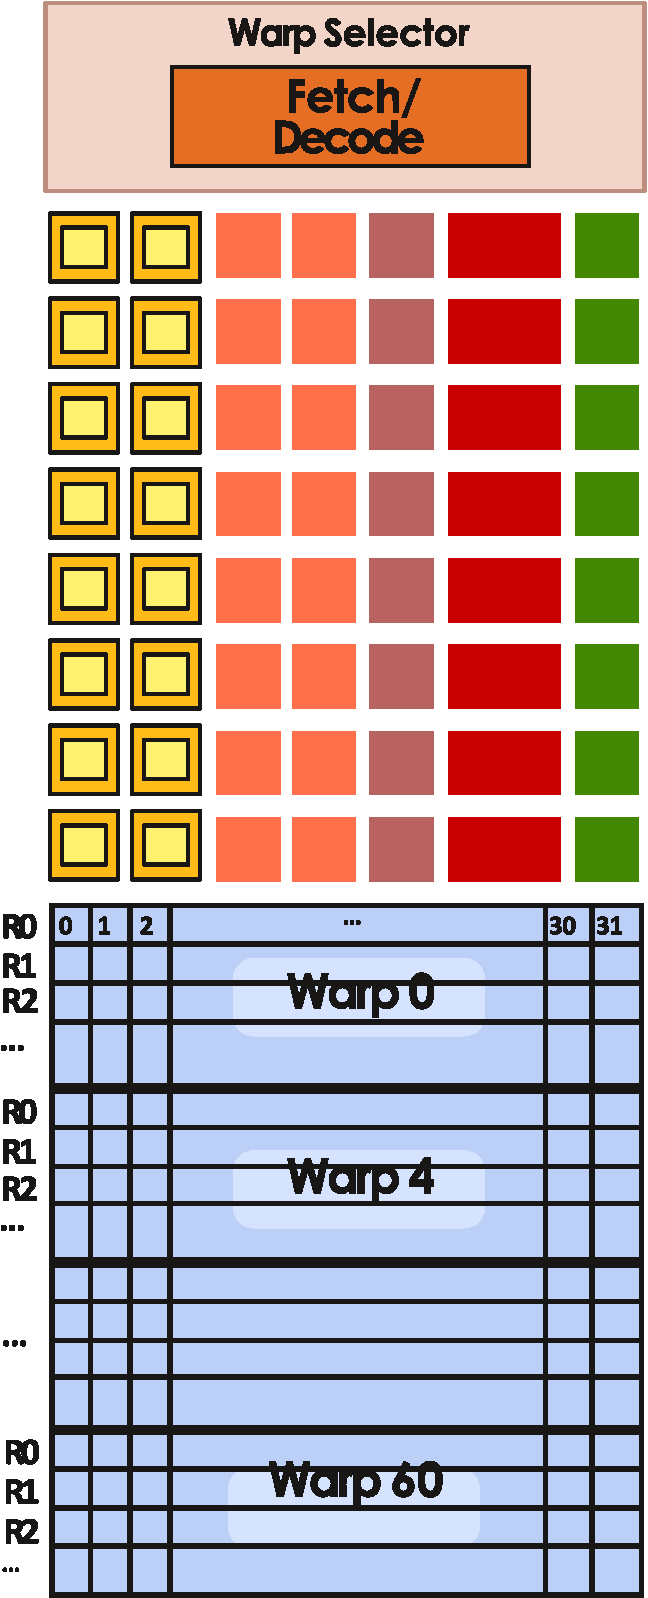
\includegraphics[width=.4\textwidth]{img/nvidia-v100-sm-1.pdf}
    \caption{A \dquotes{sub-core} of the NVIDIA V100 Streaming Multiprocessor (SM) architecture.}
\end{figure}

\begin{flushleft}
    \textcolor{Green3}{\faIcon{question-circle} \textbf{What is a Warp?}}
\end{flushleft}
A \definition{Warp} is a \textbf{group of 32 threads that execute the same instruction at the same time}. \textbf{Threads within a block are divided into warps}. For example, a block of 256 threads would have 8 warps (256 threads / 32 threads per warp). \textbf{Each SM} in the V100 \textbf{can schedule and interleave the execution of up to 16 warps}. This means that multiple warps can be executed simultaneously, improving the overall throughput of the GPU. Finally, each warp has some registers to store the data needed by the threads.

\newpage

\begin{flushleft}
    \textcolor{Green3}{\faIcon{question-circle} \textbf{How is a Warp executed?}}
\end{flushleft}
\textbf{Threads within a warp execute the same instruction simultaneously}, taking advantage of \textbf{SIMD execution} to improve performance. 

\highspace
\textbf{When threads within a warp do not share the same instruction, it results in divergent execution, which can degrade performance due to the need to serialize instructions}. However, the \textbf{check} of the same instruction by the 32 threads is done \textbf{dynamically by the GPU hardware}. Finally, although not part of CUDA, understanding warps is critical to optimizing CUDA programs on modern NVIDIA GPUs.

\highspace
\begin{figure}[!htp]
    \centering
    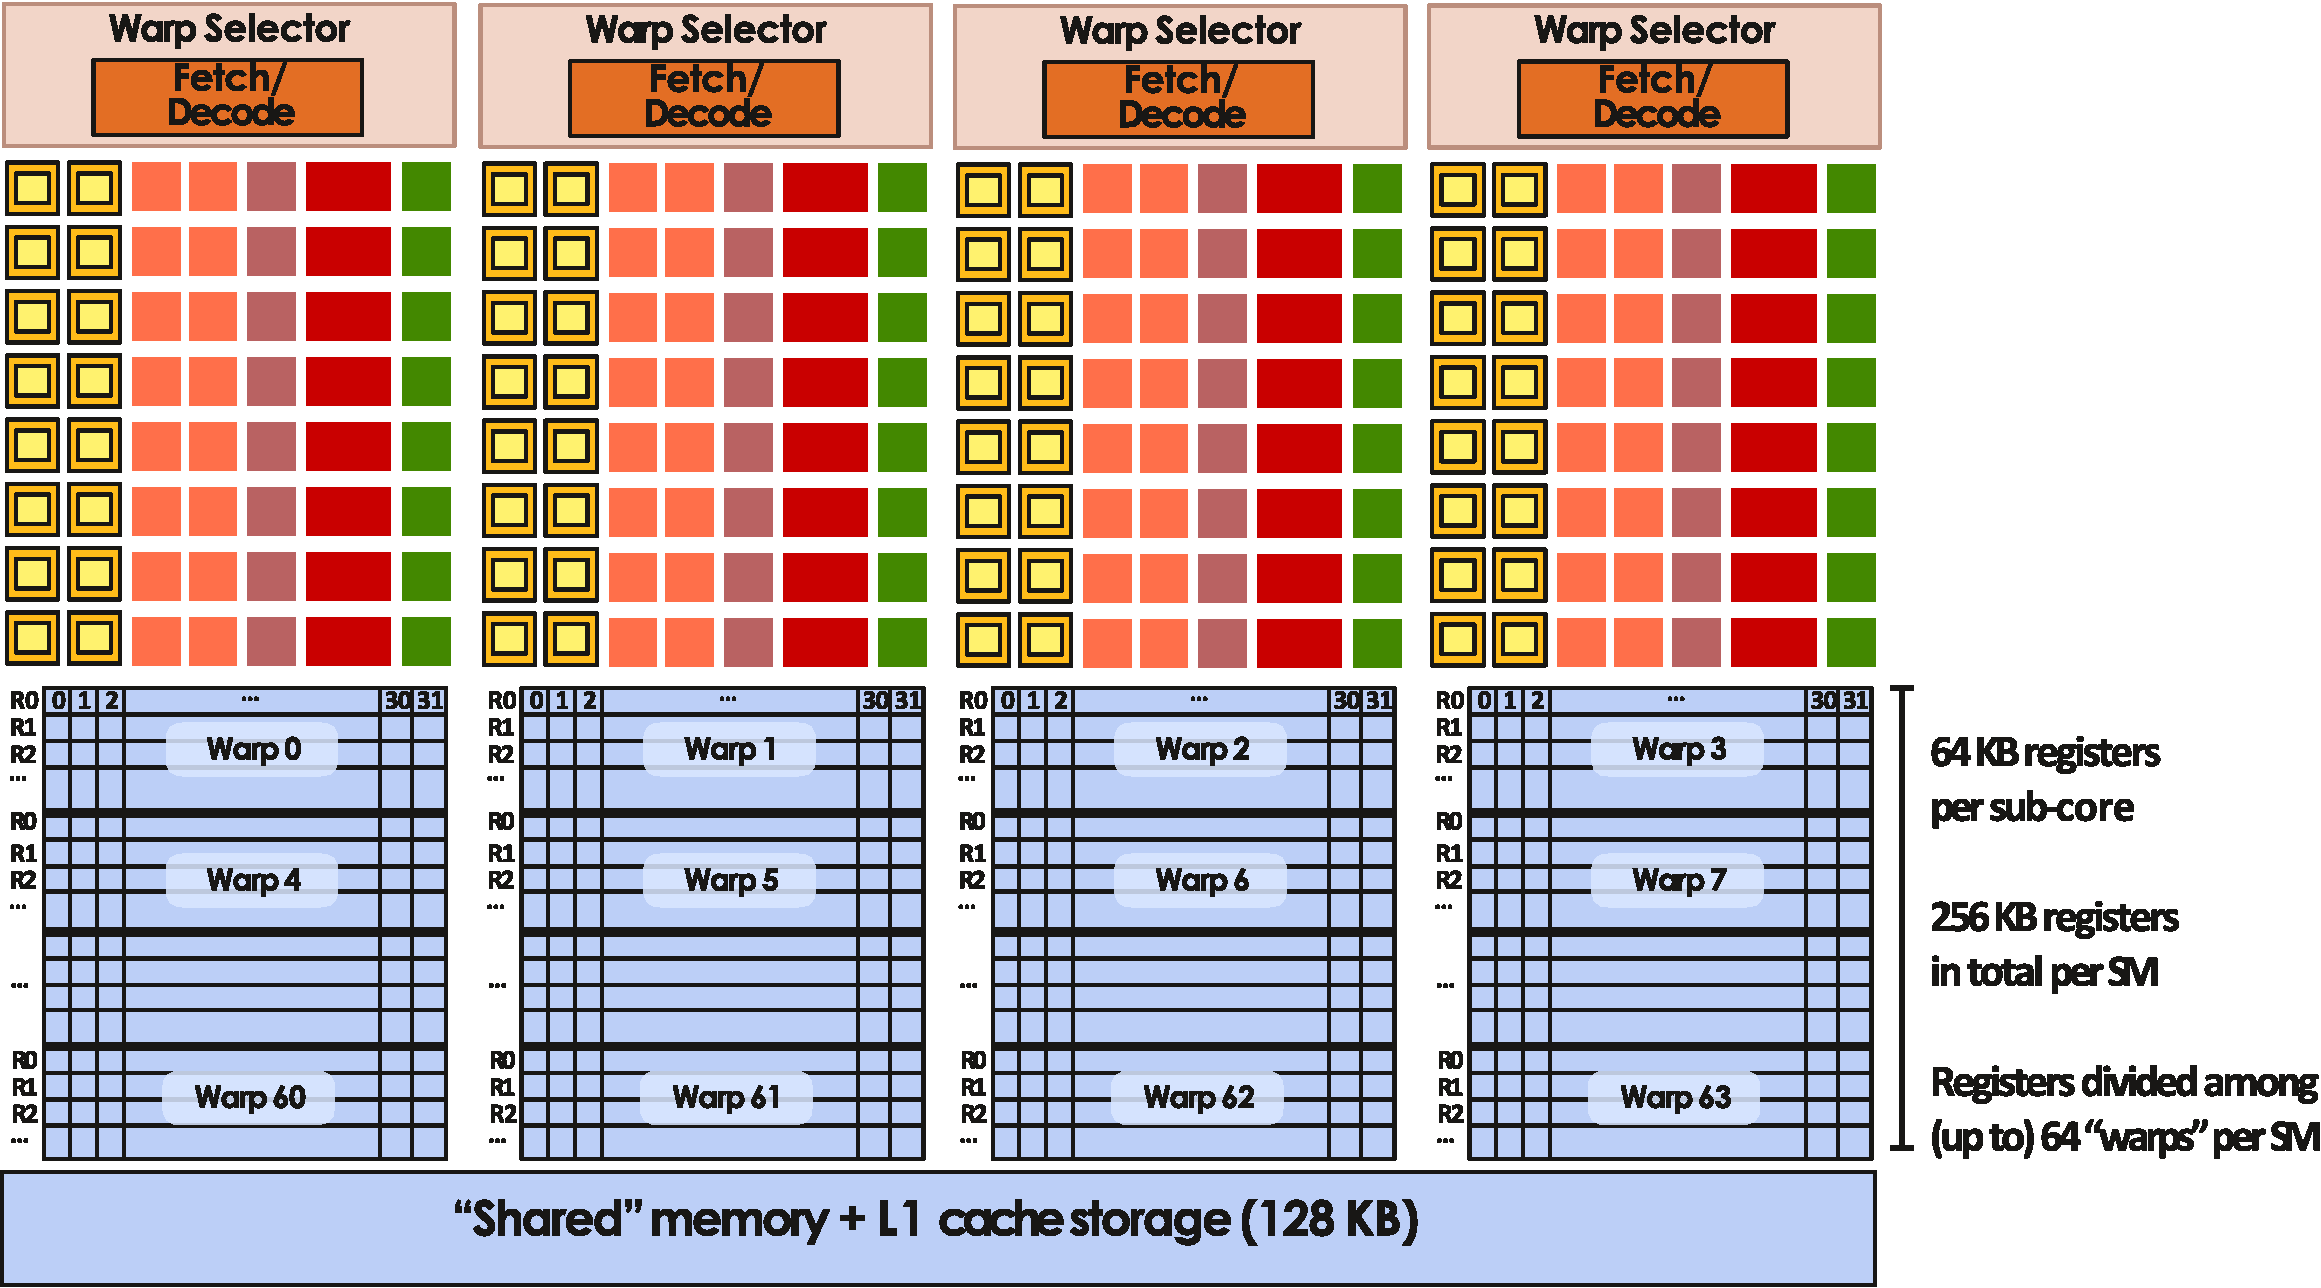
\includegraphics[width=\textwidth]{img/nvidia-v100-sm-2.pdf}
    \caption{A NVIDIA V100 Streaming Multiprocessor (SM) architecture.}
\end{figure}

    \subsubsection{Running a CUDA program on a GPU}\label{subsubsection: Running a CUDA program on a GPU}

The following section is dedicated to understanding the execution of the \dquotes{convolve} kernel on a fictitious dual-core GPU. In other words, we present an example of a kernel function execution (and therefore GPU-executed) that implements a convolution operation. It also aims to show why memory management is also fundamental inside the GPU.

\highspace
The kernel execution requirements for this explanation are:
\begin{itemize}
    \item Each \textbf{thread block} must execute \textbf{128 CUDA threads}.
    \item Each thread block must allocate $130 \times \texttt{sizeof(float)} = 520$ bytes of shared memory. In other words, \textbf{each thread block requires 520 bytes of shared memory}.
\end{itemize}
Let's take an array of size $N$ as \textbf{input} to the kernel function. When the kernel function is executed (launched), it generates thousands of thread blocks because the array size $N$ is assumed to be very large.

\begin{lstlisting}[language=C++]
#define THREADS_PER_BLK 128
convolve<<<(N/THREADS_PER_BLK), THREADS_PER_BLK>>>(N, input_array, output_array);
\end{lstlisting}

\noindent
Where:
\begin{itemize}
    \item \texttt{N/THREADS\_PER\_BLK} is the number of blocks per grid.
    \item \texttt{THREADS\_PER\_BLK} is the number of threads per block, 128 CUDA threads in our case.
\end{itemize}
The \textbf{main task} of the \emph{GPU Work Scheduler} is to \textbf{manage the two available cores} (let's say Core 0 and Core 1), where each core has its own \textbf{Fetch/Decode units}, \textbf{execution context storage} for 384 CUDA threads (12 warps), and \textbf{shared memory storage} (1.5 KB).

\highspace
Note that this architecture has fictitious cores that are smaller than V100 SM cores, with fewer execution units, less support for active warps, and less shared memory.

\begin{figure}[!htp]
    \centering
    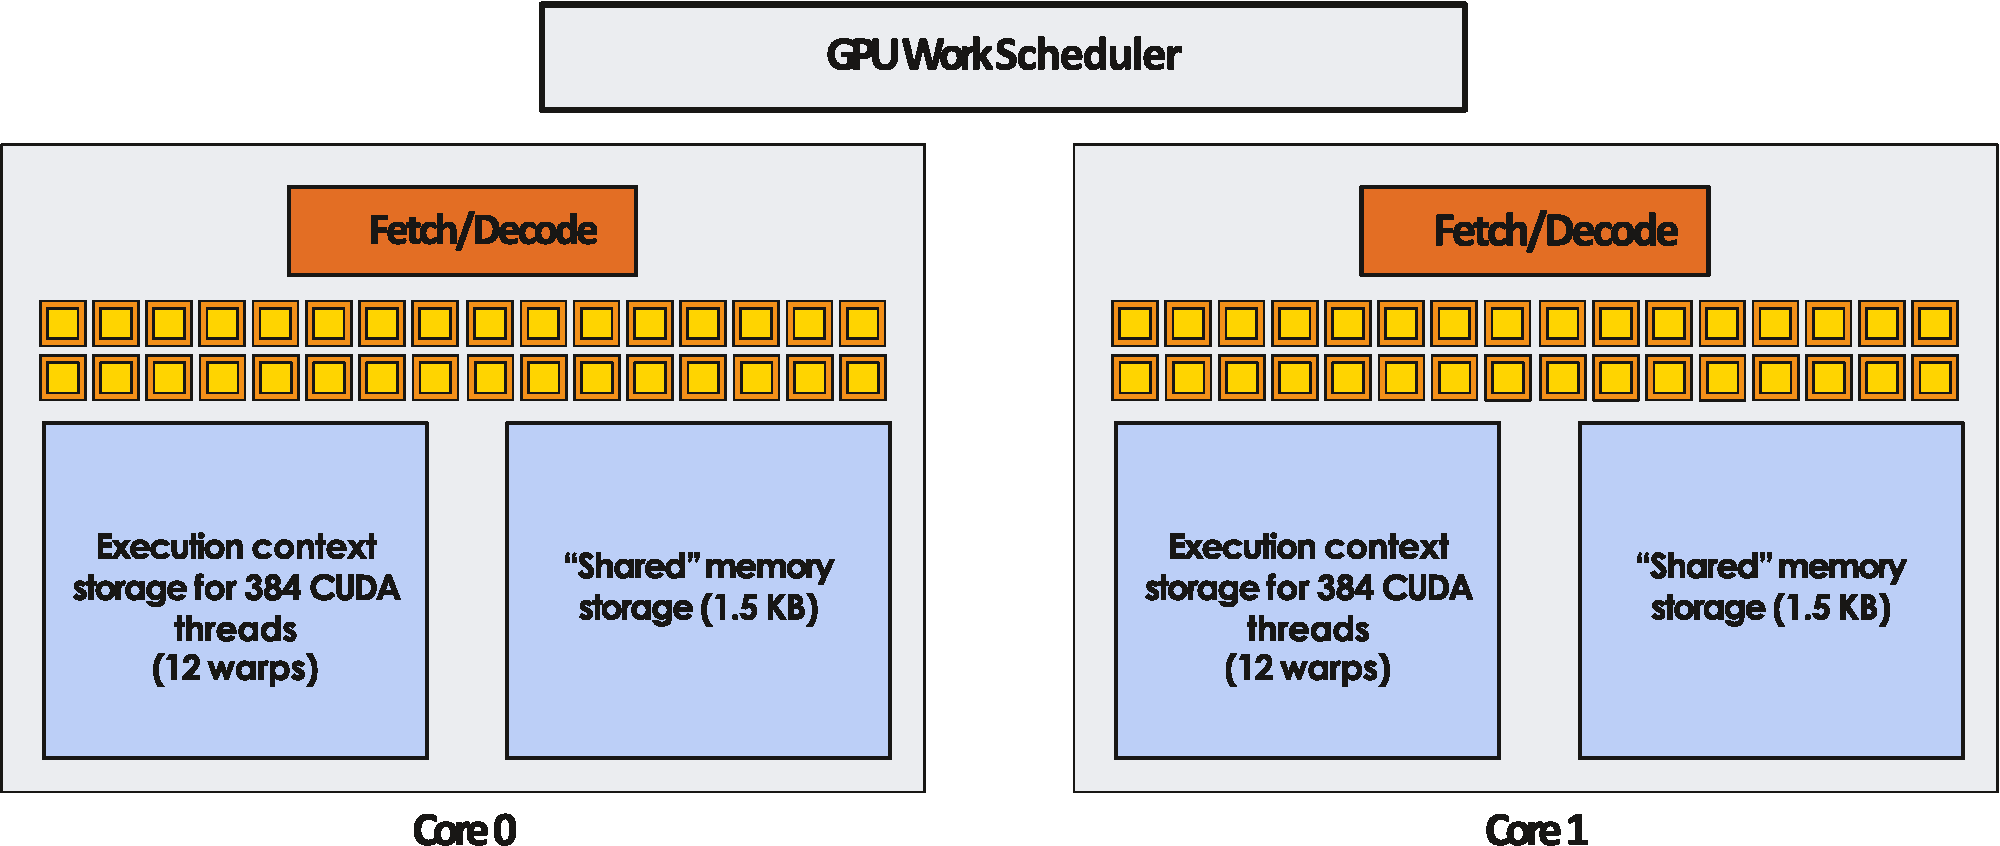
\includegraphics[width=\textwidth]{img/cuda-convolve-kernel-1.pdf}
\end{figure}

\newpage

\begin{flushleft}
    \textcolor{Green3}{\faIcon{tachometer-alt} \textbf{Execution}}
\end{flushleft}
\begin{enumerate}
    \item The \textbf{host} (CPU) \textbf{sends a command to the CUDA device} (GPU), which is the execution of the kernel function.
    \begin{itemize}
        \item \textbf{Execute}: convolve (kernel function)
        \item \textbf{Args}:
        \begin{itemize}
            \item \texttt{N} $= 128'000$
            \item \texttt{input\_array}
            \item \texttt{output\_array}
        \end{itemize}
        \item \textbf{Number of blocks}: 1000. Note that the number of blocks is given by the formula:
        \begin{equation*}
            \dfrac{
                \texttt{N}
            }{
                \texttt{THREADS\_PER\_BLK}
            }
        \end{equation*}
        Therefore, the size of the array is easily calculated as:
        \begin{equation*}
            \dfrac{\texttt{N}}{128} = 1000 \: \Rightarrow \: \texttt{N} = 128 \times 1000 = 128'000
        \end{equation*}
    \end{itemize}


    \item The \emph{scheduler} maps \emph{block 0} to \emph{Core 0}, reserving execution contexts for 128 threads and 520 bytes of shared memory to meet requirements.
    \begin{figure}[!htp]
        \centering
        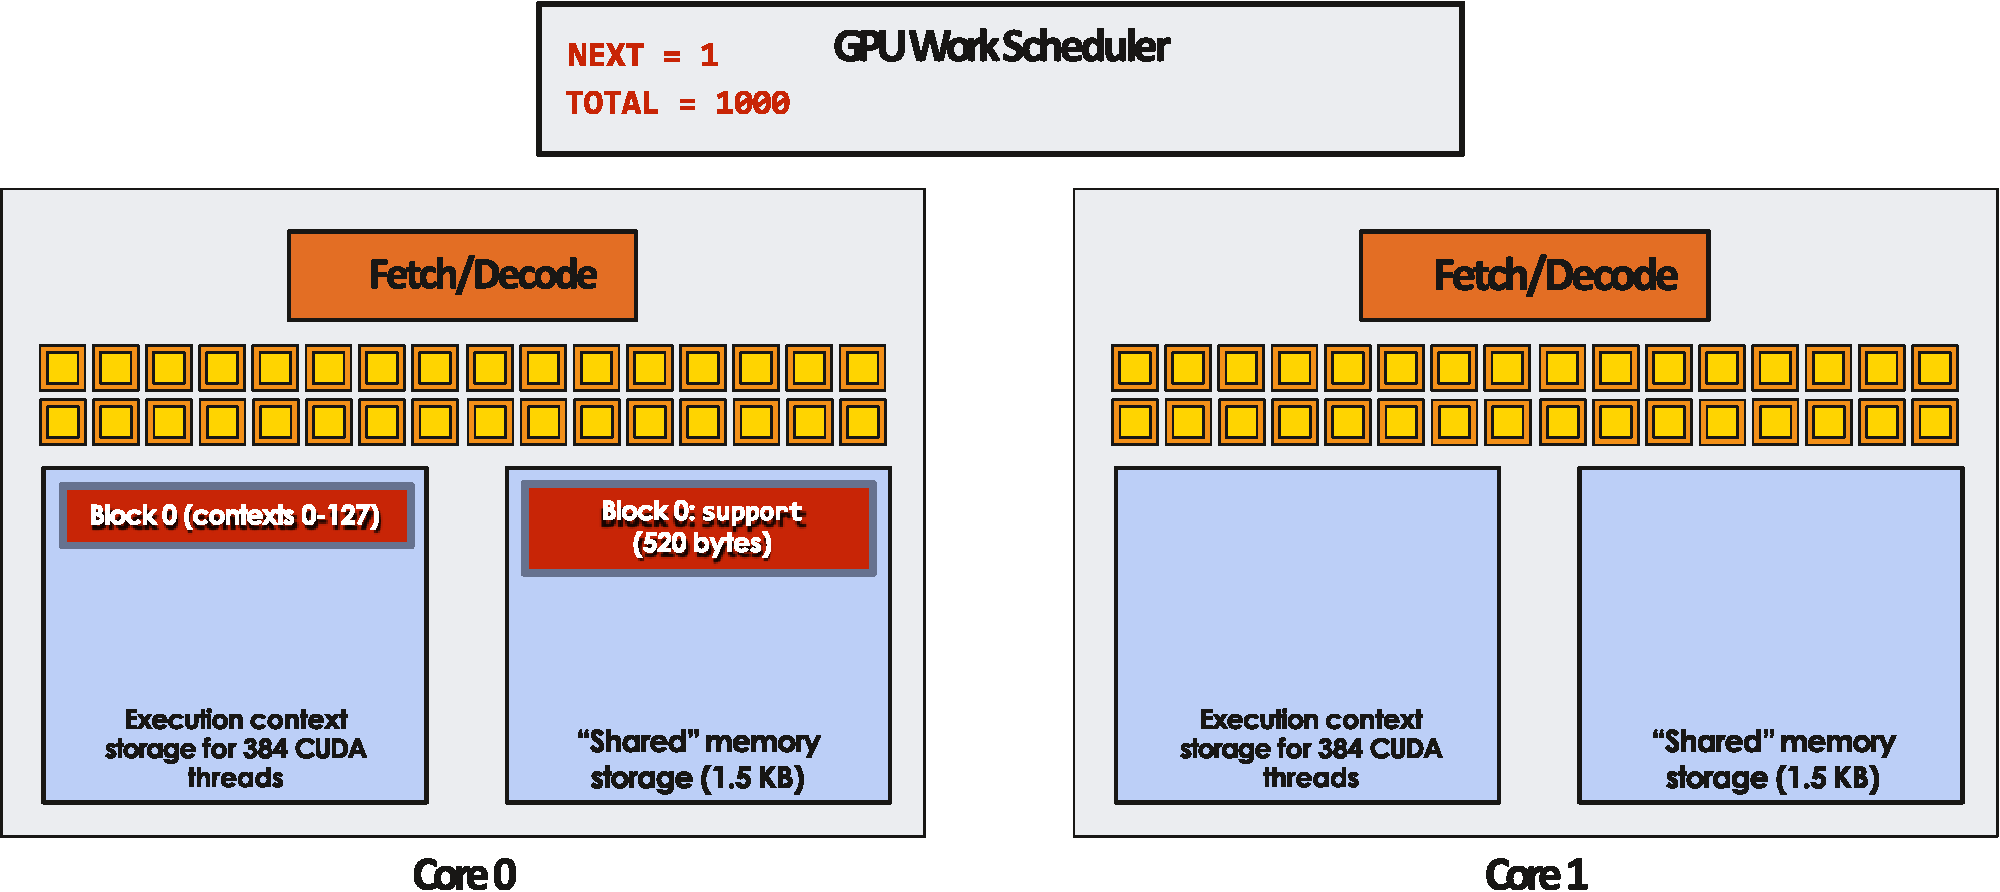
\includegraphics[width=\textwidth]{img/cuda-convolve-kernel-2.pdf}
    \end{figure}

    \newpage

    \item The \emph{scheduler} continues to map blocks to available execution contexts, so it now maps \emph{block 1} to \emph{Core 1}. This shows \textbf{interleaved mapping} (where the scheduler maps blocks to available execution contexts across different cores, ensuring efficient use of resources).\index{CUDA Interleaved Mapping}
    \begin{figure}[!htp]
        \centering
        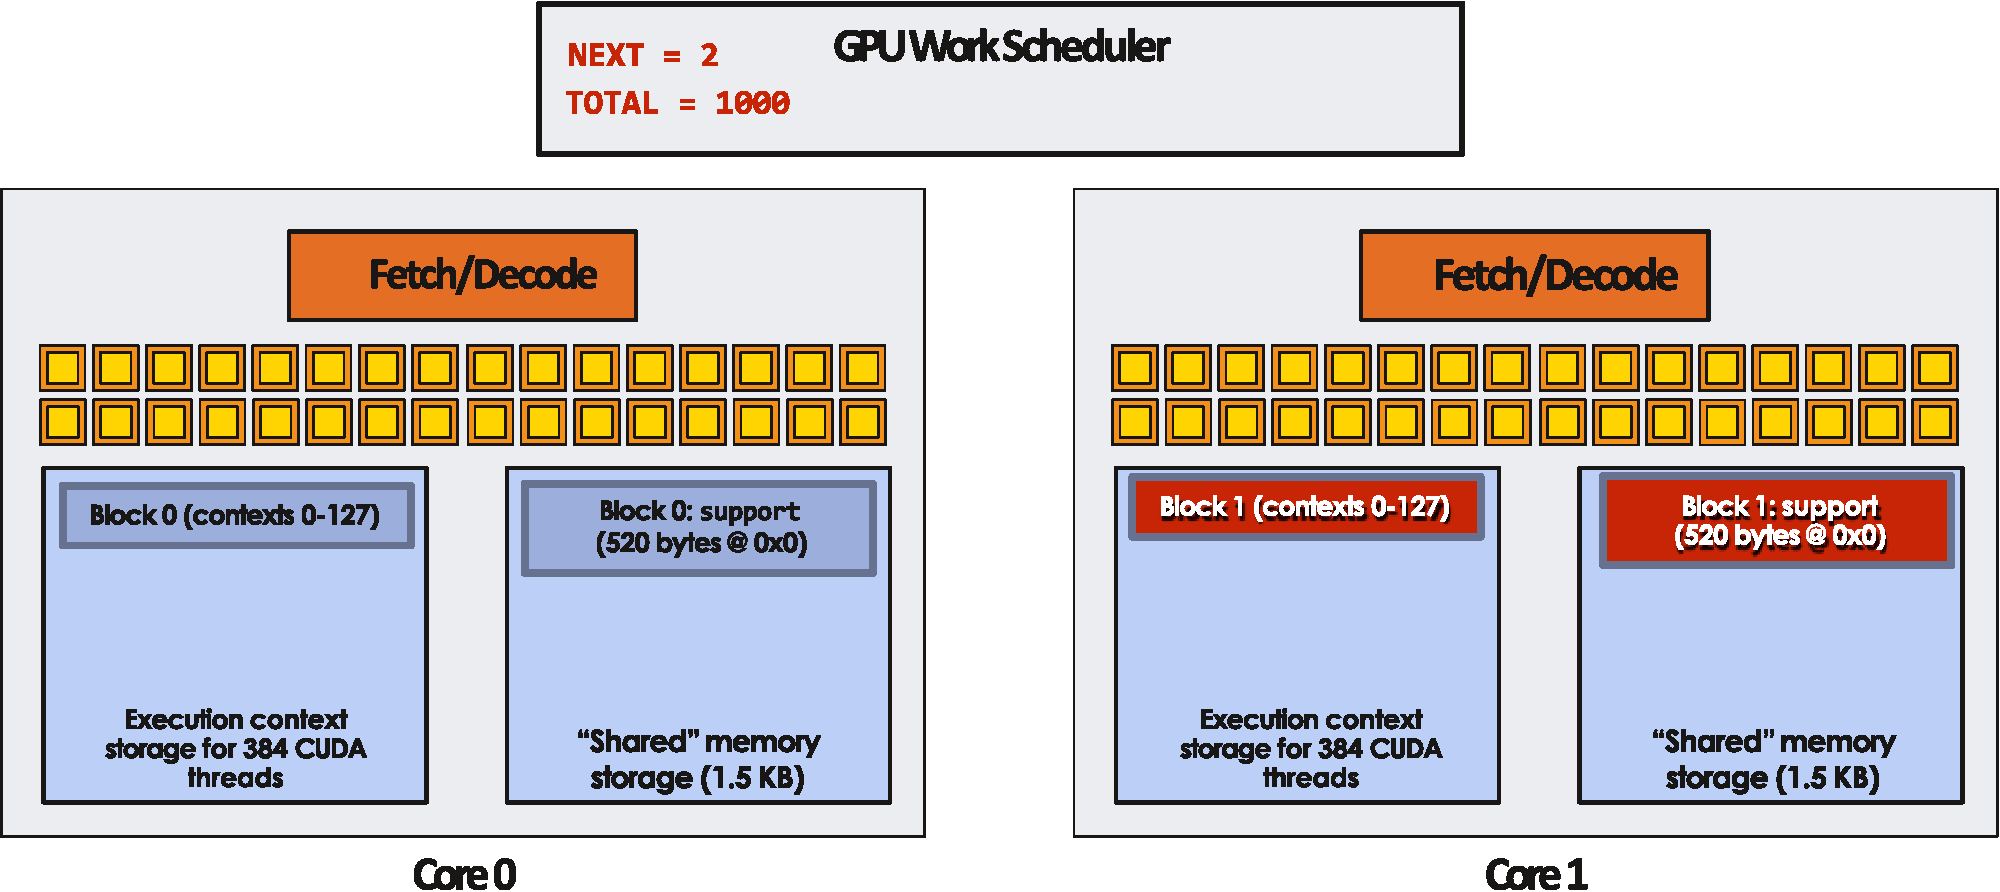
\includegraphics[width=\textwidth]{img/cuda-convolve-kernel-3.pdf}
    \end{figure}


    \item As in the previous step, there is a interleaved mapping phenomena. The scheduler maps \emph{block 2} to \emph{Core 0}. But now the shared memory (\emph{Core 0}) is saturated because three concurrent blocks allocate $520 \texttt{ bytes} \times 3 = 1.56 \texttt{ KB} > \text{limit } (1.5 \texttt{ KB})$.
    \begin{figure}[!htp]
        \centering
        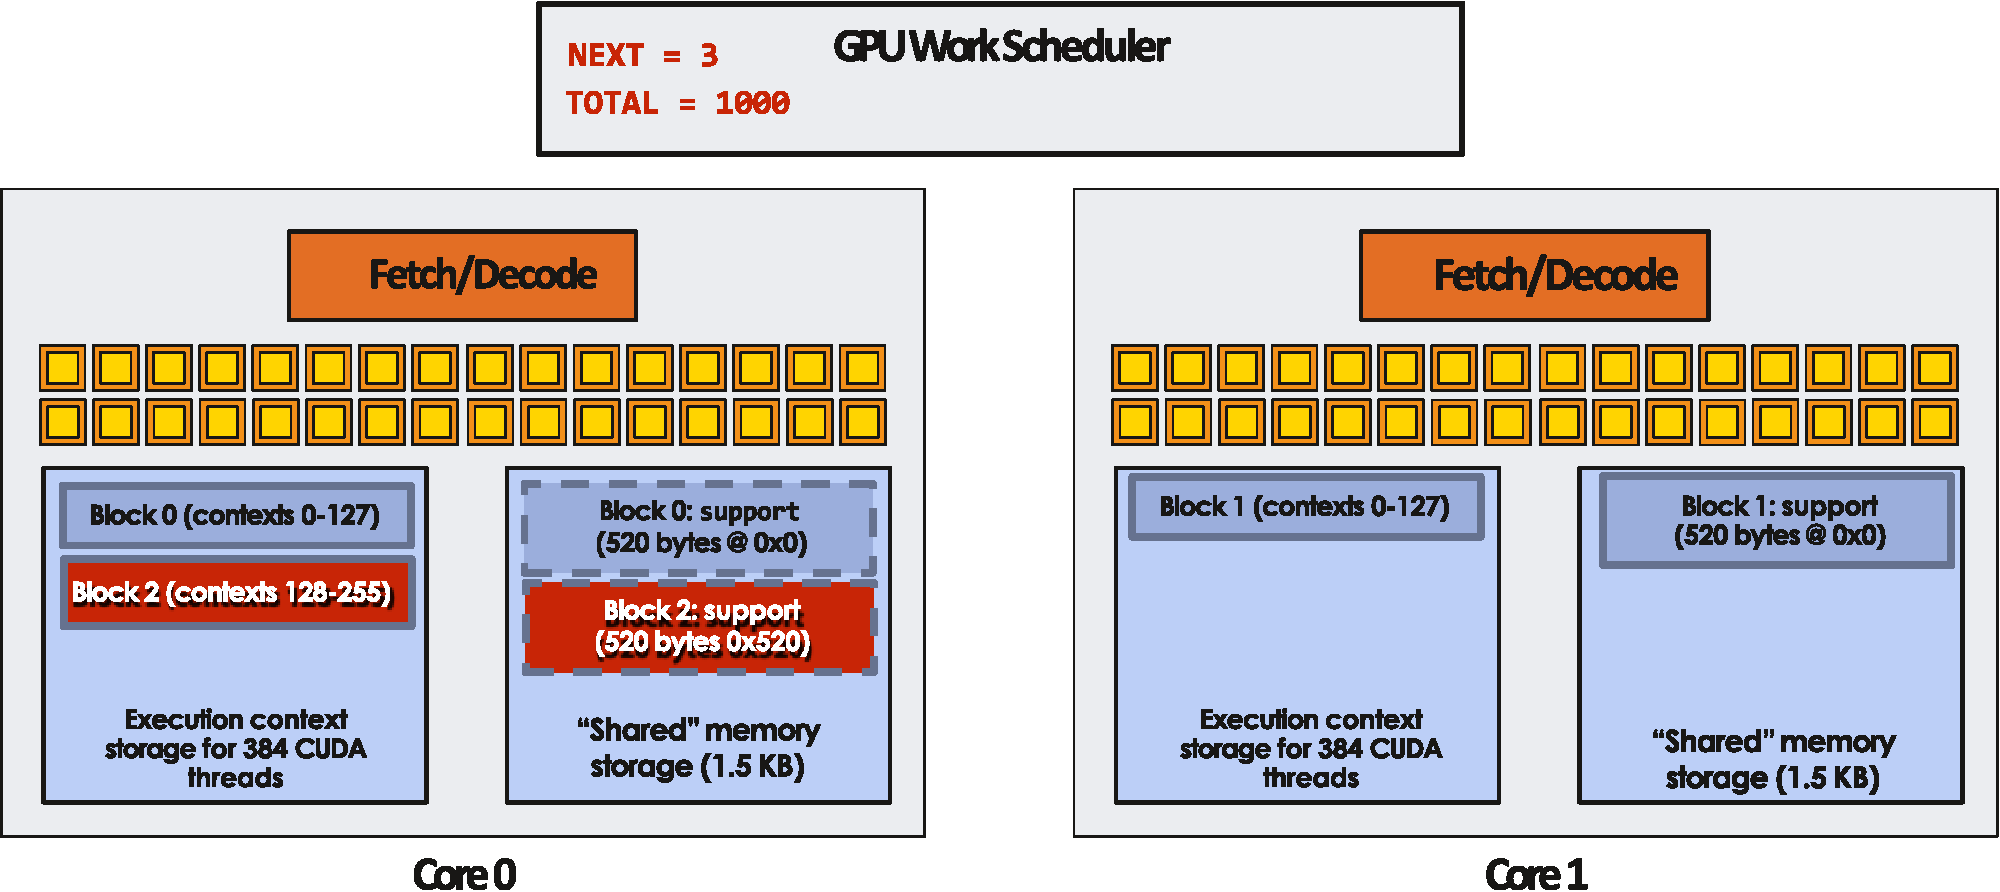
\includegraphics[width=\textwidth]{img/cuda-convolve-kernel-4.pdf}
    \end{figure}

    \newpage

    \item The scheduler assigns \emph{block 3} to \emph{Core 1}. But now the shared memory of \emph{Core 1} is also \textbf{saturated}, because three concurrent blocks allocate $520 \texttt{ bytes} \times 3 = 1.5 \texttt{ KB} > \text{limit } (1.5 \texttt{ KB})$. So we can say that only two thread blocks fit on one core.
    \begin{figure}[!htp]
        \centering
        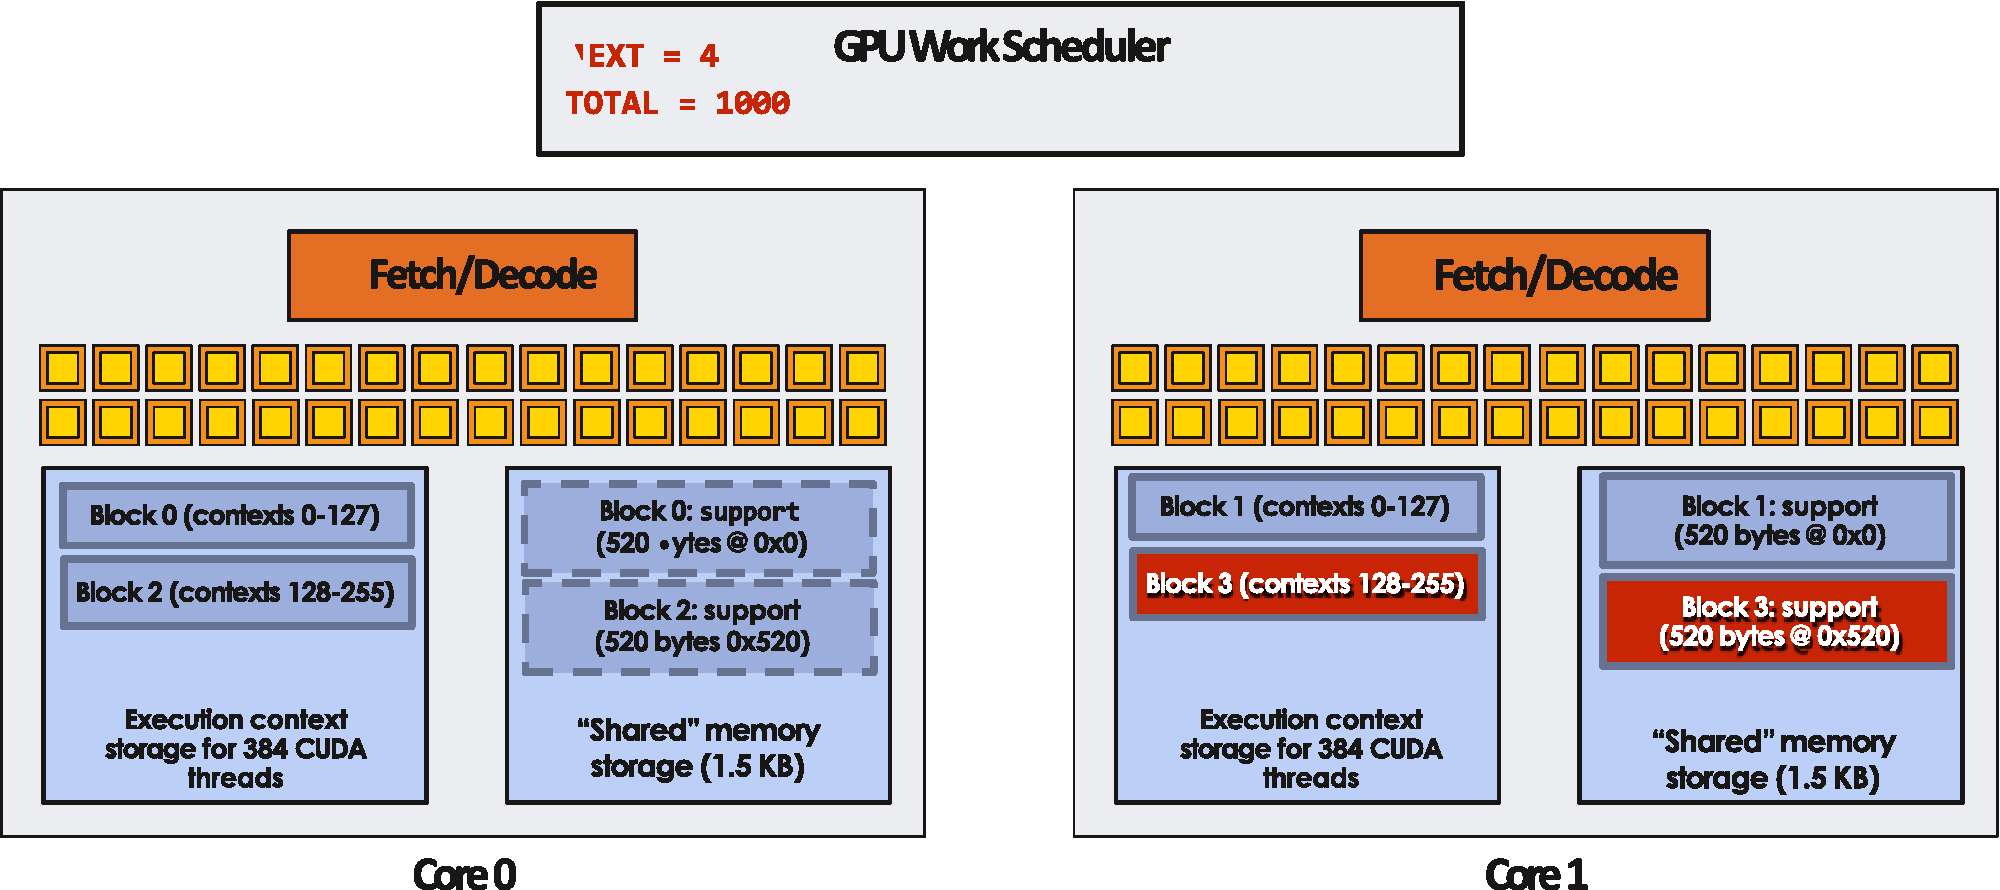
\includegraphics[width=\textwidth]{img/cuda-convolve-kernel-5.pdf}
    \end{figure}

    \item The scheduler waits for a task to complete on a block. The following figure shows \emph{block 0} completing on \emph{Core 0}. Now \emph{Core 0} is ready to host execution blocks again.
    \begin{figure}[!htp]
        \centering
        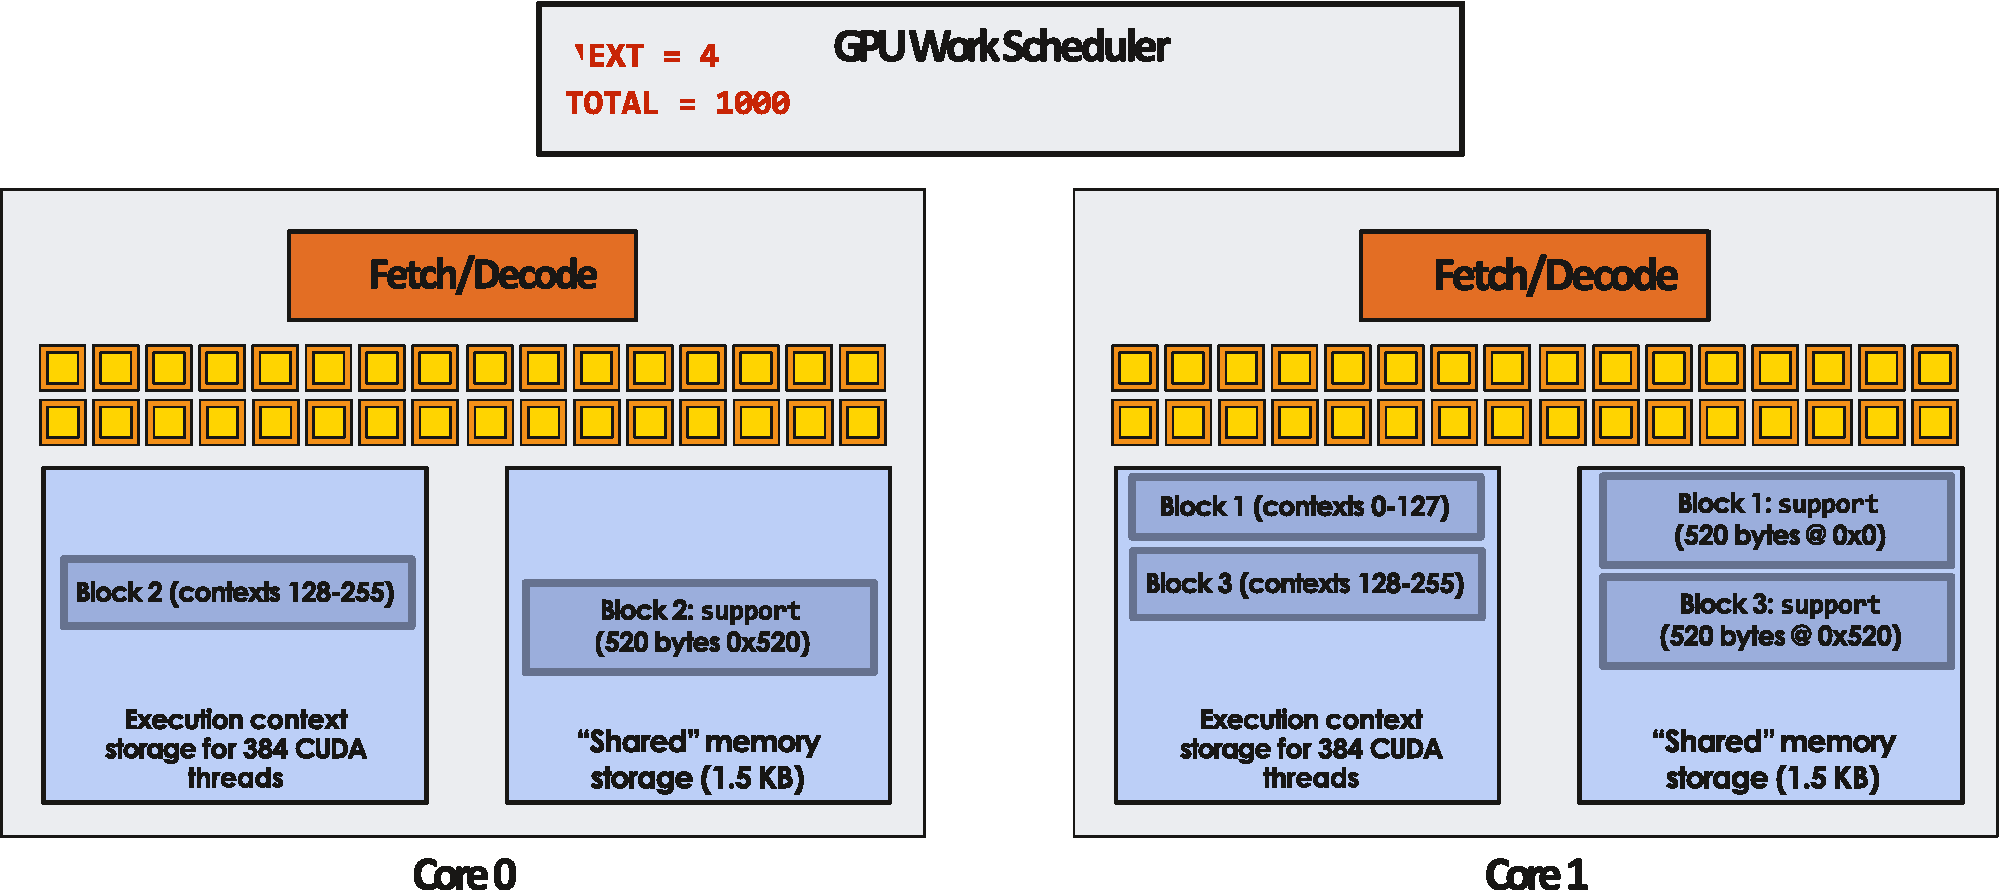
\includegraphics[width=\textwidth]{img/cuda-convolve-kernel-6.pdf}
    \end{figure}

    \newpage

    \item When the task is complete, the scheduler assigns \emph{block 4} to \emph{Core 0}.
    \begin{figure}[!htp]
        \centering
        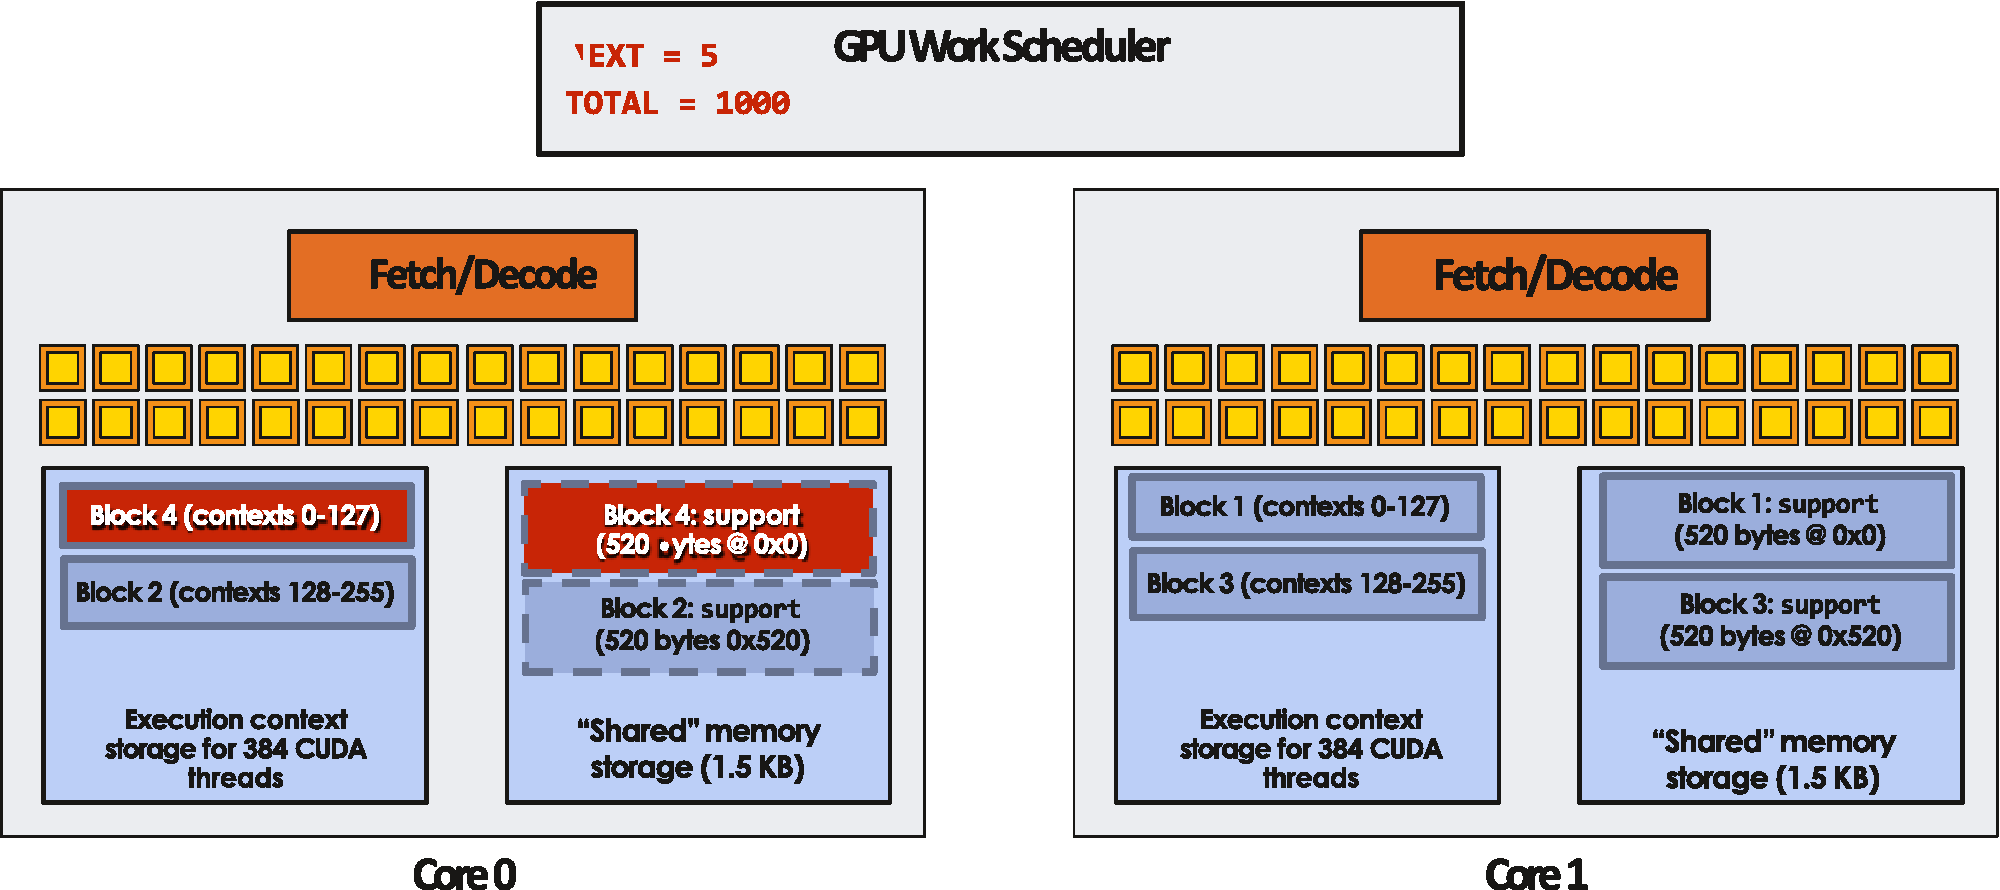
\includegraphics[width=\textwidth]{img/cuda-convolve-kernel-7.pdf}
    \end{figure}

    \item Thread \emph{block 2} completes on \emph{Core 0}.
    \begin{figure}[!htp]
        \centering
        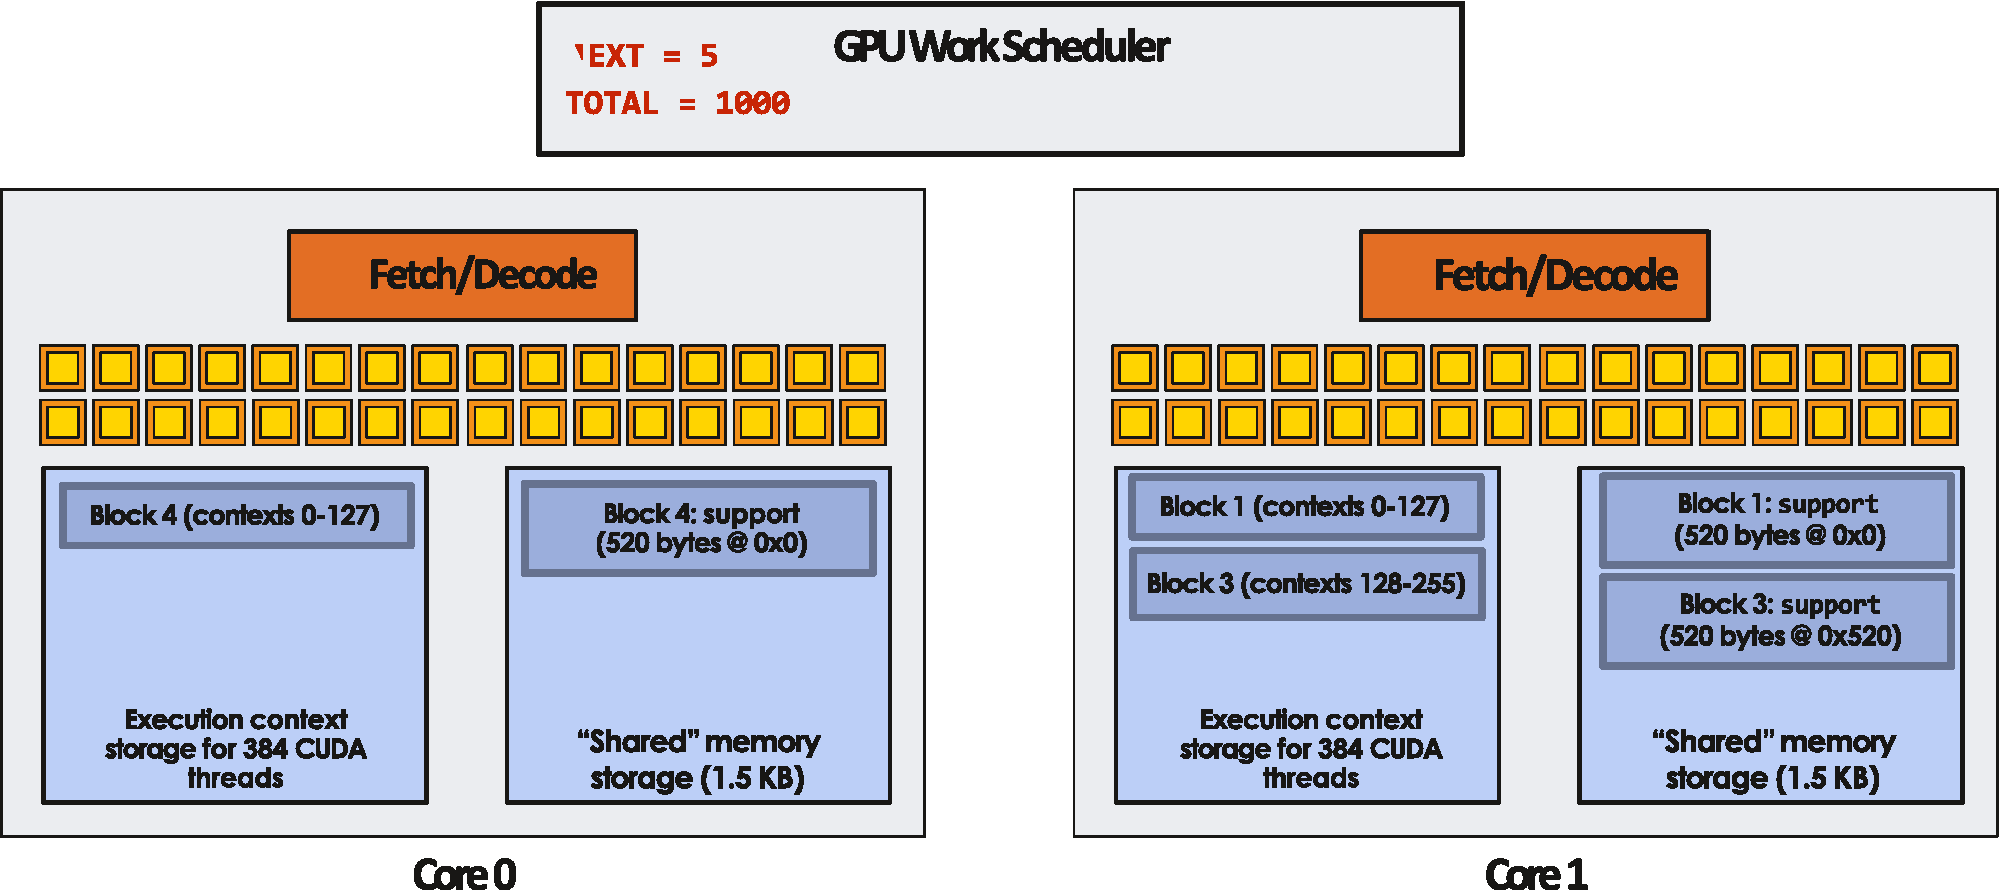
\includegraphics[width=\textwidth]{img/cuda-convolve-kernel-8.pdf}
    \end{figure}

    \item Finally, thread \emph{block 5} is scheduled on \emph{Core 0}.
    \begin{figure}[!htp]
        \centering
        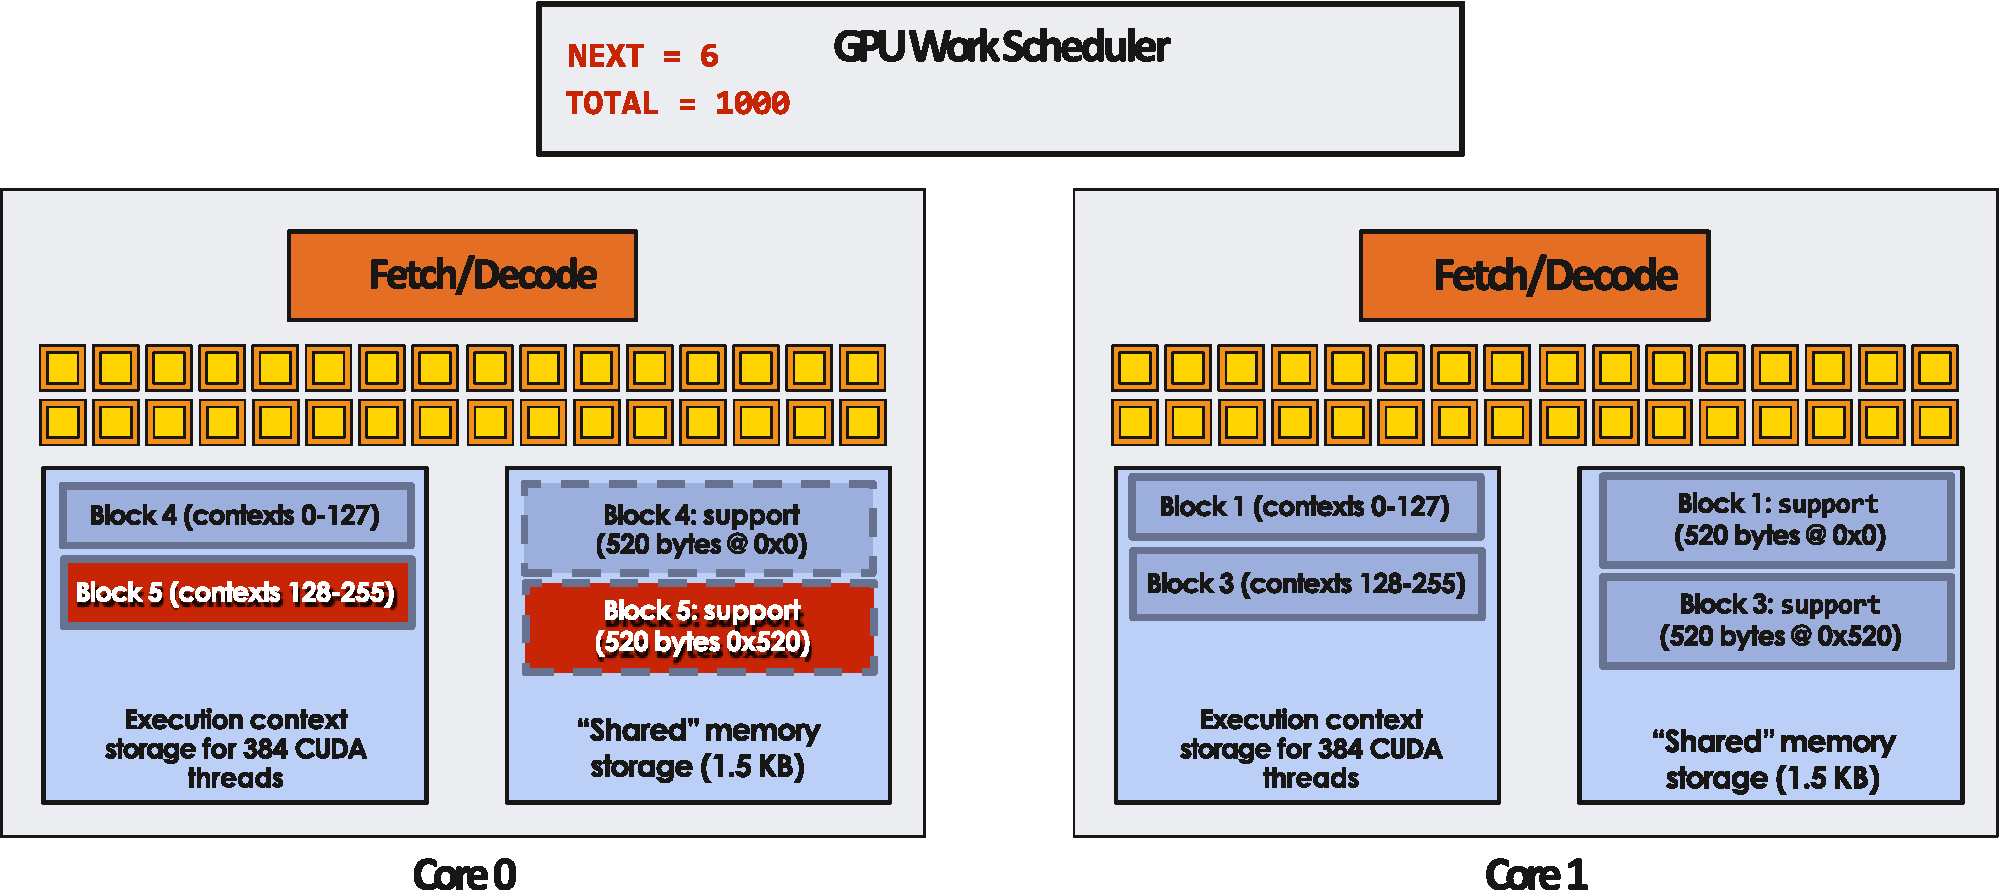
\includegraphics[width=\textwidth]{img/cuda-convolve-kernel-9.pdf}
    \end{figure}
\end{enumerate}
The explanation is intended to illustrate a phenomenon where the GPU scheduler has to manage limited shared memory resources across multiple thread blocks.
\begin{itemize}
    \item \textbf{Shared Memory Saturation}: When a GPU core's shared memory is fully occupied by existing thread blocks, new thread blocks cannot be scheduled until sufficient shared memory is freed up by the completion of some of the current thread blocks.
    
    \item \textbf{Idle Periods}: While the scheduler is waiting for shared memory to become available, the \textbf{GPU cores may be idle}. This doesn't mean the entire GPU is idle, but certain cores may not have new blocks to execute until resources are freed up.

    \item \textbf{Resource Contention}: This example shows how shared memory contention can affect the scheduling efficiency of a GPU. \textbf{Efficient use of shared memory is critical to maximizing GPU performance}.

    \item The concept of \textbf{resource contention}, whether it be shared memory, registers or other resources, is well known in parallel computing and GPU programming. It highlights the \textbf{importance of optimizing memory usage to avoid bottlenecks and ensure efficient execution}.
\end{itemize}
The example demonstrates how GPUs must juggle limited resources while maximizing throughput, a key aspect of parallel computing. By showing that the scheduler must wait before allocating new blocks, it emphasizes the \textbf{importance of careful resource management in kernel design and execution}.

    \subsubsection{Implementation of CUDA abstractions}

We assume that we have a fictitious \textbf{Streaming Multiprocessor (SM) core} (Figure \ref{fig: A sub-core of the NVIDIA V100 Streaming Multiprocessor (SM) architecture} page \pageref{fig: A sub-core of the NVIDIA V100 Streaming Multiprocessor (SM) architecture}, same as NVIDIA V100, page \pageref{subsubsection: NVIDIA V100 Streaming Multiprocessor (SM)}) with only \textbf{four warps} of parallel execution in hardware. So there are 4 warps times 32 threads, and \textbf{128 threads} can be executed in parallel each time.

\begin{figure}[!htp]
    \centering
    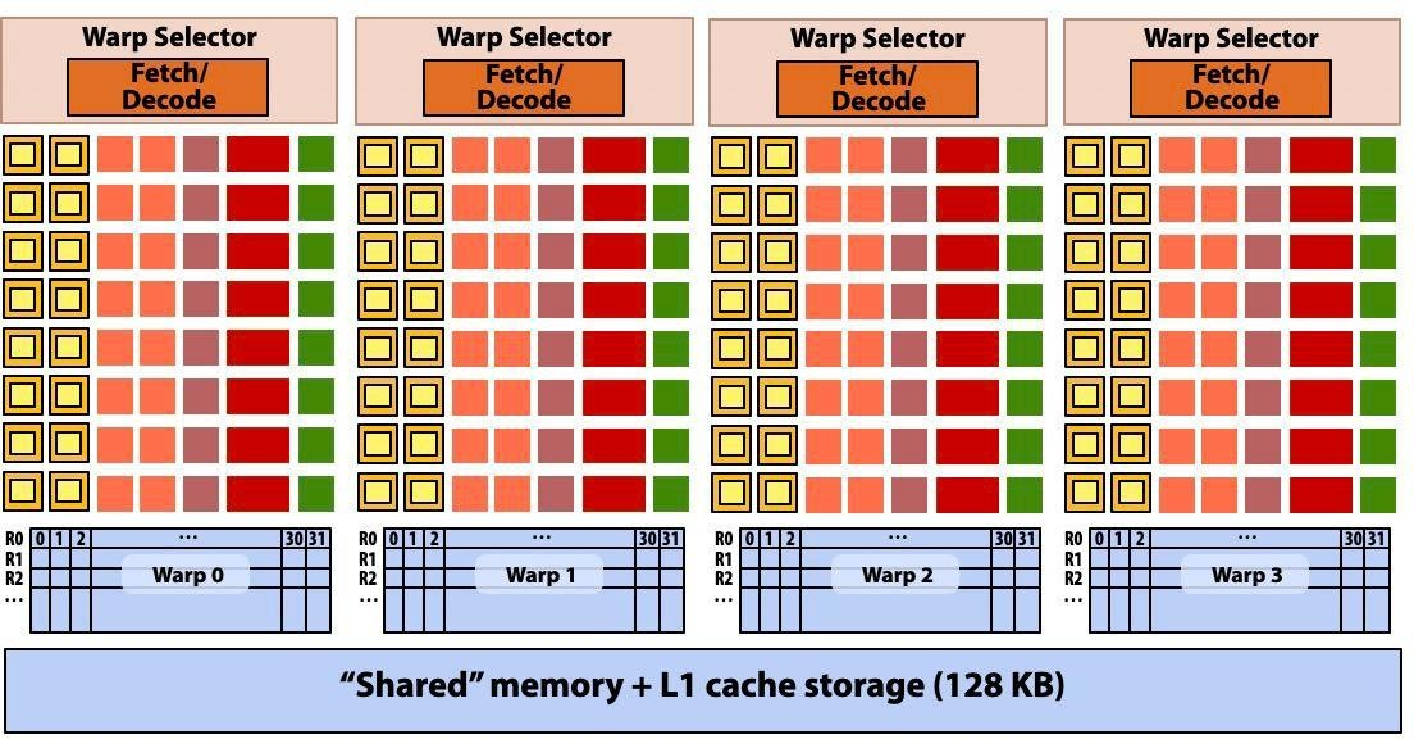
\includegraphics[width=\textwidth]{img/cuda-abs-1.pdf}
    \caption{Streaming Multiprocessor (SM) core, with 4 warps and 128 threads in total.}
\end{figure}

\begin{flushleft}
    \textcolor{Green3}{\faIcon{question-circle} \textbf{Why allocating all threads in a block might be inefficient}}
\end{flushleft}
Now imagine we want to run a CUDA program where a thread \textbf{block} consists of \textbf{256 CUDA threads}, even though our GPU architecture can \emph{only} execute 128 threads at a time. A naive implementation might execute the entire CUDA block by executing four warps (threads 0-127) to completion, and then execute the next four warps (threads 128-255) to completion. This \textbf{sequential execution of warps can lead to inefficiencies} because \textbf{there may be idle periods where some warps are stalled waiting for memory accesses or synchronization points}.

\highspace
\begin{flushleft}
    \textcolor{Green3}{\faIcon{check-circle} \textbf{Use interleaving execution}}
\end{flushleft}
A good alternative is to use interleaved execution. \definition{Interleaved execution} means that the \textbf{GPU schedules warps so that they overlap}. While some warps are waiting for memory access or synchronization, \textbf{others can execute}. This overlapping helps to \textbf{hide latencies} and \textbf{keep the GPU cores busy}.

\highspace
However, \textbf{CUDA kernels can create dependencies between threads in a block}. To manage these dependencies, the programmer can use the function \texttt{\_\_syncthreads()} to synchronize threads within a block. \texttt{\_\_syncthreads()} ensures that \textbf{all threads in the block reach the synchronization point before any thread can continue}. This means that threads 128-255 cannot continue until threads 0-127 reach the synchronization point.

\highspace
\begin{flushleft}
    \textcolor{Green3}{\faIcon{check-circle} \textbf{Why interleaving execution is optimal when there are dependencies}}
\end{flushleft}
If we run four warps to completion before starting the next four, we \textbf{may not be using shared resources} (such as shared memory and execution units) efficiently. This can also \textbf{lead to scenarios where some warps are stalled indefinitely waiting for other warps to reach synchronization points}, causing potential \textbf{\underline{deadlocks}} or inefficiencies.

By interleaving the execution of warps, the GPU can better manage thread dependencies, hide latencies, and make more efficient use of its resources.

\highspace
\begin{lstlisting}[language=C++]
#define THREADS_PER_BLK 256

__global__ void convolve(int N, float* input, float* output)
{
    __shared__ float support[THREADS_PER_BLK * 2];
    int index = blockIdx.x * blockDim.x + threadIdx.x;

    support[threadIdx.x] = input[index];
    if (threadIdx.x < N) {
        support[
            THREADS_PER_BLK + threadIdx.x
        ] = input[index + THREADS_PER_BLK];
    }

    __syncthreads();

    float result = 0.0f; // thread-local
    for (int i = 0; i < 5; i++)
        result += support[threadIdx.x + i];

    output[index] = result;
}
\end{lstlisting}

\begin{flushleft}
    \textcolor{Red2}{\faIcon{book} \textbf{Summary}}
\end{flushleft}
\begin{enumerate}
    \item Thread \textbf{blocks} can be \textbf{scheduled in any order by the system}.
    \begin{itemize}
        \item The system assumes no dependencies between blocks.
        \item Blocks are logically concurrent, similar to ISPC tasks (Implicit SPMD Program Compiler, page \pageref{definitionbox: Implicit SPMD Program Compiler (ISPC)}).
    \end{itemize}

    \item \textbf{CUDA threads in the same block run concurrently} (live at the same time).
    \begin{itemize}
        \item When a block begins executing, all threads exist and have register state allocated.
        \item A \textbf{CUDA thread block is an SPMD} (Single Program, Multiple Data) \textbf{program}, similar to an ISPC gang of program instances.
        \item Threads in a thread block are concurrent, cooperating \dquotes{workers}.
    \end{itemize}

    \newpage

    \item \textbf{CUDA implementation}.
    \begin{itemize}
        \item An NVIDIA GPU warp has performance characteristics \emph{similar} to an ISPC gang of instances.
        \item All warps in a thread block are scheduled onto the same SM (Streaming Multiprocessor), allowing for high-bandwidth, low-latency communication through shared memory variables.
        \item When all threads in a block complete, block resources (shared memory allocations, warp execution contexts) become available for the next block.
    \end{itemize}
\end{enumerate}
 
    \subsubsection{Advanced thread scheduling}

The \emph{main goal} of this section is to show how a CUDA kernel uses hardware execution resources: thread block allocation to execution resources, execution resource capacity constraints, and zero-overhead thread scheduling.

\highspace
In general, \textbf{CUDA thread blocks execute independently and can run in any order}. The hardware is \textbf{free to assign blocks to any processor at any time}. This flexibility allows the GPU to optimize resource utilization and balance the load. A kernel (the function that runs on the GPU) scales to any number of parallel processors. This means that the same code can run efficiently on GPUs with different numbers of cores.

\highspace
\begin{wrapfigure}{r}{0.35\textwidth}
    \centering
    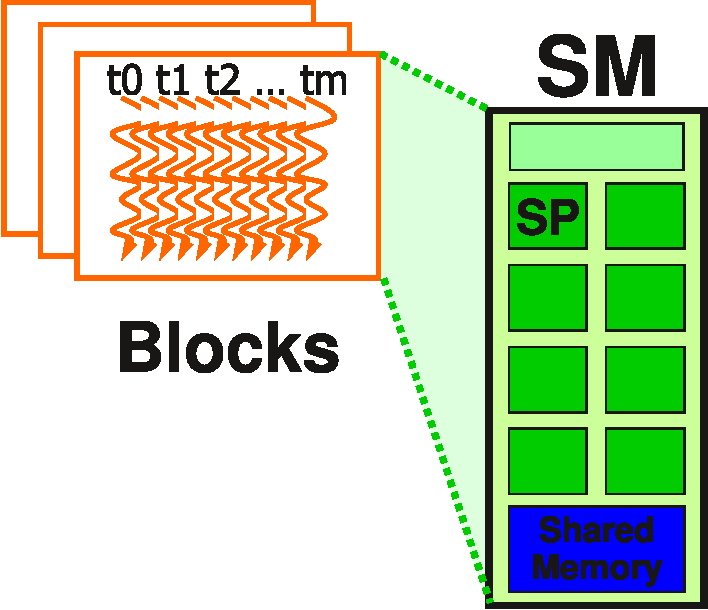
\includegraphics[width=0.34\textwidth]{img/executing-thread-blocks-1.pdf}
\end{wrapfigure}
Thread blocks are the basic unit of work in CUDA and are assigned to SMs in block granularity (as we saw in Chapter \ref{subsubsection: Running a CUDA program on a GPU}). This means that a \textbf{thread block cannot be split across multiple SMs, but is executed entirely within a single SM}. Each SM has a \emph{limit} on the number of threads and thread blocks it can support simultaneously. For example, the \textbf{Volta SM can handle up to 2048 threads}. The number of blocks an SM can hold depends on the number of threads per block:
\begin{itemize}
    \item If a block has 256 threads, up to 8 blocks can fit ($256 \times 8 = 2048$ threads).
    \item If a block has 512 threads, only 4 blocks can fit ($512 \times 4 = 2048$ threads).
\end{itemize}
The \textbf{SM manages the indexes of the threads and blocks assigned to it}, enabling scheduling and execution.

\highspace
\begin{flushleft}
    \textcolor{Green3}{\faIcon{bookmark} \textbf{Von Neumann model with SIMD units}}
\end{flushleft}\index{Von Neumann model with SIMD units}
The \textbf{Von Neumann Model} consists of a Control Unit, ALU (Arithmetic Logic Unit), Registers, Memory, and I/O components that work in a sequential manner. However, when we \textbf{integrate SIMD} (Single Instruction, Multiple Data) units into the model, we add the \textbf{ability to process multiple data items simultaneously using a single instruction}.

\highspace
As we have explained in the section \ref{subsubsection: Single Instruction, Multiple Data (SIMD) processor} page \pageref{subsubsection: Single Instruction, Multiple Data (SIMD) processor}, SIMD allows the same operation to be performed on multiple pieces of data in parallel. This means a Control Unit (CU) sends the same instruction to multiple ALUs, each working on different data at the same time.

\newpage

\begin{flushleft}
    \textcolor{Green3}{\faIcon{bookmark} \textbf{Von Neumann model with SIMD units in GPUs}}
\end{flushleft}
The \textbf{architecture uses SIMD units to execute multiple threads in parallel}, making GPUs highly efficient at tasks involving large data sets, such as image processing, matrix multiplication, and other data-parallel computations.

\highspace
In \textbf{CUDA}, \textbf{warps} (groups of 32 threads) are \textbf{executed in a SIMD fashion}. \textbf{All threads in a warp perform the same operation, but on different pieces of data}. This is critical for speeding up computations that need to process large amounts of data in parallel. SIMD capabilities allow GPUs to efficiently handle large numbers of parallel tasks, making them far more powerful than traditional CPUs for certain workloads, such as graphics rendering and scientific computing.

\begin{figure}[!htp]
    \centering
    \includegraphics[width=.6\textwidth]{img/von-neumann-model-with-simd-1.pdf}
    \caption{Von Neumann model with SIMD units.}
\end{figure}
    \subsubsection{Memory and Data Locality in Depth}

In CUDA programming, understanding memory and data locality is crucial for achieving high performance. 

\highspace
\begin{flushleft}
    \textcolor{Green3}{\faIcon{question-circle} \textbf{Why Memory Hierarchy and Data Locality Matter}}
\end{flushleft}
We propose a piece of code of a kernel function where there is a computation of the blur in an image:
\begin{lstlisting}[language=C++]
// get the average of the surrounding 2xBLUR_SIZE x 2xBLUR_SIZE box
for(int blurRow = -BLUR_SIZE; blurRow < BLUR_SIZE+1; ++blurRow)
{
    for(int blurCol = -BLUR_SIZE; blurCol < BLUR_SIZE+1; ++blurCol)
    {
        int curRow = Row + blurRow;
        int curCol = Col + blurCol;
        // Verify we have a valid image pixel
        if(curRow > -1 && curRow < h && curCol > -1 && curCol < w)
        {
            pixVal += in[curRow * w + curCol]; $\label{code: access global var}$
            // keep track of number of pixels
            // in the accumulated total
            pixels++;
        }
    }
}

// write our new pixel value out
out[Row * w + Col] = (unsigned char)(pixVal / pixels);
\end{lstlisting}

\noindent
The \textbf{code accesses global memory for input matrix elements}. This is evident from the line \ref{code: access global var} where \texttt{in} is likely a pointer to the global memory holding the image data. Therefore, each thread accesses global memory to read the pixel values within a 2xBLUR\_SIZE x 2xBLUR\_SIZE box around the current pixel.
\begin{itemize}
    \item Each \textbf{memory access is 4 bytes} per floating point addition.
    \item The \textbf{memory bandwidth is 4 bytes per second per FLOP}, 4B/s of memory bandwidth/FLOPS.
\end{itemize}
Assuming a GPU with a peak floating point rate of 1,600 GigaFLOPS and a DRAM bandwidth of 600 GB/s, then 1,600 GigaFLOPS would require 6,400 GB/s of memory bandwidth to achieve the peak FLOPS. However, the 600 GB/s memory bandwidth limits execution to 150 GFLOPS, which is only 9.3\% of the peak floating point execution rate. \textbf{To get close to the 1,600 GigaFLOPS, it is necessary to drastically cut down memory accesses}.

\highspace
In other words, there is an \textbf{evident Memory Bandwidth Bottleneck}. Even with a high peak floating-point rate, the actual performance can be limited by memory bandwidth (to achieve 1,600 GigaFLOPS, the kernel would require 6,400 GB/s of memory bandwidth, but the available bandwidth is only 600 GB/s).

\newpage

\noindent
Therefore, it is important to understand that \textbf{minimizing global memory access and optimizing data locality are essential strategies in CUDA programming to achieve high performance}. This is because accessing global memory often results in high latency, which can significantly degrade the performance of our GPU application.
\begin{itemize}
    \item \definition{Global memory access}. Global memory is the largest and slowest memory available on a GPU. \textbf{Frequent accesses to global memory can cause significant performance bottlenecks due to high latency}.
    
    \item \definition{Bandwidth and Latency}. While global memory provides high bandwidth, the latency associated with \textbf{accessing it can slow overall performance}, especially when multiple threads are accessing it simultaneously.
    
    \item \definition{Memory hierarchy}. GPUs have a hierarchical memory structure that includes registers, shared memory, and global memory. \textbf{Using a proper memory structure} can improve performance and reduce memory bandwidth. We discussed these topics in Section \ref{CUDA memory: Types of CUDA device memory models visible to kernels}, page \pageref{CUDA memory: Types of CUDA device memory models visible to kernels}.

    \item \definition{Data Locality and Caching}. Optimizing data locality (keeping frequently accessed data close to where it is processed) is key to improving performance. \textbf{Using shared memory to cache data that is accessed multiple times by threads can significantly reduce the need for global memory accesses}.
\end{itemize}
    \subsubsection{Tiling Technique}

The \definition{Tiling Technique}, also known as \textbf{\emph{blocked matrix multiplication}} or \textbf{\emph{tiling}}, is a strategy to \textbf{enhance the performance of matrix computations by optimizing memory access patterns}. It leverages shared memory in CUDA to reduce the number of global memory accesses, improving efficiency and throughput. A lot of parallel algorithms adopt the tiling technique.

\highspace
\begin{flushleft}
    \textcolor{Green3}{\faIcon{question-circle} \textbf{What is Tiling?}}
\end{flushleft}
Tiling can be thought of as the \textbf{process of breaking a large matrix into smaller sub-matrices} (called \emph{tiles} or blocks) \textbf{that can fit into faster}, \textbf{limited shared memory}. The \underline{main goal} of tiling is to:
\begin{itemize}
    \item \textbf{Minimize} slower \textbf{global memory accesses};
    \item \textbf{Maximize} the \textbf{use of faster shared memory}.
\end{itemize}
Instead of a large matrix, we can think of the global memory contents as tiles and focus the computation of CUDA threads on one or a small number of tiles at a time.

\highspace
\begin{flushleft}
    \textcolor{Green3}{\faIcon{book} \textbf{Great analogy to understand the basic concept of Tiling}}
\end{flushleft}
Reducing the number of vehicles in a congested traffic system can significantly improve the delays experienced by all vehicles. This is analogous to carpooling for commuters. We can image:
\begin{itemize}
    \item \textbf{Drivers}: represent \emph{threads accessing their memory data operands}.
    \item \textbf{Cars}: represent \emph{memory access requests}.
\end{itemize}
Just as carpooling reduces the number of cars on the road, tiling reduces the number of global memory accesses by loading data into shared memory. The result is a reduction in traffic (memory access requests) and an obvious improvement in overall efficiency.

\highspace
Unfortunately, just like in real life, there are some problems. For example, there are the \textbf{challenges of carpooling}. In fact, some carpools are easier to organize than others because the participants need to have similar work schedules. So certain vehicles may be more suitable for carpooling. However, other \textbf{commuters may have different needs}, \textbf{so the number of carpools may increase and there is a risk of increasing traffic again}.

\highspace
Similar challenges exist in tiling calculations. Some computations may be easier to tile based on data access patterns and the nature of the computation. \textbf{Organizing data and computations efficiently to fit into tiles may be more challenging for certain algorithms}. So what is the \textbf{general euristic to adopt in order to use the tiling technique} or not? In general, it is:
\begin{itemize}
    \item[\textcolor{Green3}{\faIcon{check}}] \textbf{\textcolor{Green3}{\textbf{Good}} to use} tiling when people have similar schedule. In computing, is good \textbf{when threads have \emph{similar access timing}}.

    \item[\textcolor{Red2}{\faIcon{times}}] \textbf{\textcolor{Red2}{\textbf{Bad}} to use} tiling when people have very different schedule. In computing, is bad \textbf{when threads have very \emph{different timing}}.
\end{itemize}
But synchronization is also important. Just as workers' schedules must be aligned for effective carpooling, \textbf{threads} in parallel computing \textbf{must be synchronized} for efficient execution. Efficient data access and memory usage depend on synchronized operations to reduce latency and improve performance. The following figure shows synchronization between multiple threads.

\begin{figure}[!htp]
    \centering
    \includegraphics[width=.8\textwidth]{img/cuda-tiling-1.pdf}
    \caption{Barrier Synchronization for Tiling.}
\end{figure}

\noindent
On the left are multiple threads (\texttt{Thread 0}, \texttt{Thread 1}, \texttt{Thread 2}, \dots, \texttt{Thread N-1}) progressing over time. The wave represents when each thread reaches its barrier on the code; at that point, the thread must wait until all threads have arrived before it can continue. This ensures that all threads are synchronized at certain points during execution. Execution of all threads resumes when the last thread (in the picture, \texttt{Thread N-2}) reaches the barrier.

\highspace
\textbf{Synchronization is fundamental in the tiling technique} because it \textbf{ensures that all threads have their share of data loaded into shared memory and are ready to proceed before they perform any computations}. After the computation, they use another synchronization barrier to ensure that all threads have completed their work before moving to the next tile.

\newpage

\begin{flushleft}
    \textcolor{Green3}{\faIcon{tools} \textbf{Summary - How it works}}
\end{flushleft}
\begin{enumerate}
    \item \important{Identify a Tile}. Determine a section of global memory content that multiple threads will access. Dividing the workload into smaller tiles allows for efficient memory access and utilization of shared memory.
    \item \important{Load the Tile}. Transfer the tile from global memory to on-chip memory (shared memory). Loading data into shared memory reduces the latency associated with accessing global memory.
    \item \important{Barrier Synchronization}. Ensures that all threads are ready to begin the computation phase. It also ensures that all threads have the necessary data before starting the computation.
    \item \important{Access Data}. Multiple threads access their data from the on-chip memory. Threads perform computations using the data stored in shared memory, benefiting from its faster access time.
    \item \important{Barrier Synchronization}. Ensure all threads have completed the current phase (computations).
    \item \important{Next Tile}. Move on to the next tile and repeat the process.
\end{enumerate}

\highspace
\begin{flushleft}
    \textcolor{Green3}{\faIcon{check} \textbf{Advantages}}
\end{flushleft}
\begin{itemize}
    \item[\textcolor{Green3}{\faIcon{check}}] \textbf{Improved Memory Access Patterns}. By loading data into shared memory, the number of global memory accesses is reduced, leading to better performance.
    \item[\textcolor{Green3}{\faIcon{check}}] \textbf{Higher Computational Throughput}. Tiling helps achieve higher computational throughput by leveraging the faster shared memory.
\end{itemize}

    \paragraph{Tiled Matrix Multiplication}

In the following section, we present an \textbf{example of matrix multiplication using the tiling technique} to illustrate the efficiency improvements brought about by the tiling technique.

\highspace
\begin{flushleft}
    \textcolor{Green3}{\faIcon{book} \textbf{Traditional approach}}
\end{flushleft}
Classical matrix multiplication has the following characteristics
\begin{itemize}
    \item Each thread accesses a row of matrix $M$ and a column of matrix $N$.
    \item Each thread block accesses a strip of matrix $M$ and a strip of matrix $N$.
\end{itemize}
\begin{figure}[!htp]
    \centering
    \includegraphics[width=.8\textwidth]{img/cuda-matrix-multiplication-1.pdf}
\end{figure}
In the traditional approach, threads access data directly from global memory, which can be inefficient due to high latency.

\begin{flushleft}
    \textcolor{Green3}{\faIcon{tachometer-alt} \textbf{Tiled Matrix Multiplication}}
\end{flushleft}
\begin{enumerate}
    \item As a \textbf{first step}, since we know the problem and (ideally) how the solution is implemented, we can try to brainstorm on how to apply tiling. In general, matrix operations lend themselves well to the tiling technique. In the matrix multiplication:
    \begin{itemize}
        \item The execution of each thread can be broken into phases.
        \item The data accesses by the thread block in each phase are focused on one tile of $M$ and one tile of $N$.
        \item The tile is of \texttt{BLOCK\_SIZE} elements in each dimension.
    \end{itemize}


    \item As second step, the threads in a block participate in \textbf{loading items into shared memory using the tiling technique}.
    
    As we can see in the following figure, each thread in a block contributes to loading elements from matrices $M$ and $N$ into shared memory. Each thread is responsible for loading one element from the $M$ matrix and one element from the $N$ matrix into shared memory. This parallel loading ensures that data is moved quickly and efficiently from global memory to faster shared memory.

    \begin{figure}[!htp]
        \centering
        \includegraphics[width=.8\textwidth]{img/cuda-tiled-matrix-multiplication-1.pdf}
    \end{figure}

    The matrices $M$ and $N$ are the input and $P$ is the result matrix. Each element is indexed by $i$ and $j$ (e.g., $M_{ij}$).
    \begin{itemize}
        \item Elements of $M$ are loaded into shared memory by the threads.
        \item Similarly, elements of $N$ are loaded into shared memory.
    \end{itemize}
    This particular phase focuses on the initial loading of elements for the tile corresponding to block (0,0). Each thread in block (0,0) loads one element from $M$ and one from $N$, populating the shared memory with the necessary data for the computation.

    These steps are performed for each block of the matrices. In the following figure, we can see another step of loading into shared memory.
    \begin{figure}[!htp]
        \centering
        \includegraphics[width=.8\textwidth]{img/cuda-tiled-matrix-multiplication-4.pdf}
    \end{figure}


    \newpage
    \item After loading into shared memory, there is the loading step, done in two iterations, into the result matrix. This is only a graphical representation, because in reality this step can be merged with the execution step. This step prepares the operands to be used in the execution step.
    \begin{enumerate}
        \item In the first iteration, the elements from the shared memory $N_{0,0}, N_{0,1}$ are used against the element from the shared memory $M_{0,0}, M_{1,0}$.
        \begin{figure}[!htp]
            \centering
            \includegraphics[width=.8\textwidth]{img/cuda-tiled-matrix-multiplication-2.pdf}
        \end{figure}
        \item In the second iteration, the elements from the shared memory $N_{1,0}, N_{1,1}$ are used against the element from the shared memory $M_{0,1}, M_{1,1}$.
        \begin{figure}[!htp]
            \centering
            \includegraphics[width=.8\textwidth]{img/cuda-tiled-matrix-multiplication-3.pdf}
        \end{figure}
    \end{enumerate}
    This step is done for each block of the matrices. In the figure on the next page, we can see two more steps of the load block.
    \newpage
    \begin{figure}[!htp]
        \centering
        \includegraphics[width=.8\textwidth]{img/cuda-tiled-matrix-multiplication-5.pdf}
    \end{figure}
    \begin{figure}[!htp]
        \centering
        \includegraphics[width=.8\textwidth]{img/cuda-tiled-matrix-multiplication-6.pdf}
    \end{figure}


    \item After each load, there is the \textbf{execution phase}. In the following table, we highlight how four threads in a block perform matrix multiplication using shared memory.
    \begin{figure}[!htp]
        \centering
        \includegraphics[width=\textwidth]{img/cuda-tiled-matrix-multiplication-7.pdf}
    \end{figure}
    \newpage
    The values $\texttt{Mds}_{i,j}$ are the values loaded in the load step from global to shared memory of the $M$ matrix. The same reasoning applies to $\texttt{Nds}$.

    Once the data is loaded into shared memory, each thread uses the loaded values to update the partial product value $\texttt{PValue}$ for the resulting matrix $P$:
    \begin{itemize}
        \item $\texttt{thread}_{0,0}$:
        \begin{lstlisting}[language=C++]
$\texttt{PValue}_{0,0}$ += $\texttt{Mds}_{0,0}$ * $\texttt{Nds}_{0,0}$ + $\texttt{Mds}_{0,1}$ * $\texttt{Nds}_{1,0}$\end{lstlisting}

        \item $\texttt{thread}_{0,1}$:
        \begin{lstlisting}[language=C++]
$\texttt{PValue}_{0,1}$ += $\texttt{Mds}_{0,0}$ * $\texttt{Nds}_{0,1}$ + $\texttt{Mds}_{0,1}$ * $\texttt{Nds}_{1,1}$\end{lstlisting}
        \item $\texttt{thread}_{1,0}$:
        \begin{lstlisting}[language=C++]
$\texttt{PValue}_{1,0}$ += $\texttt{Mds}_{1,0}$ * $\texttt{Nds}_{0,0}$ + $\texttt{Mds}_{1,1}$ * $\texttt{Nds}_{1,0}$\end{lstlisting}
        \item $\texttt{thread}_{1,1}$:
        \begin{lstlisting}[language=C++]
$\texttt{PValue}_{1,1}$ += $\texttt{Mds}_{1,0}$ * $\texttt{Nds}_{0,1}$ + $\texttt{Mds}_{1,1}$ * $\texttt{Nds}_{1,1}$\end{lstlisting}
    \end{itemize}

    \item \textbf{Barrier Synchronization step}. To synchronize all threads in a block, we use the function \texttt{\_\_syncthreads()}. This function acts as a barrier synchronization, ensuring that all threads in a block reach that point before any thread can proceed.
    
    Barrier synchronization is particularly useful for coordinating the execution of tiled algorithms in phases. It is useful in:
    \begin{itemize}[label=\textcolor{Green3}{\faIcon{check}}]
        \item \textbf{Loading Phase}. Ensures that \textbf{all elements of a tile are loaded into shared memory before any computation begins}.
        \item \textbf{Computation Phase}. Ensures that \textbf{all threads have completed their computation on the current tile before moving to the next phase or tile}.
    \end{itemize}
\end{enumerate}

    \paragraph{Implementation Tiled Matrix Multiplication}

After a great explanation of how to apply the tiling technique to the matrix multiplication operation, we present the CUDA implementation. As we said, the goal of tiled matrix multiplication with CUDA is to optimize the matrix multiplication process by taking advantage of shared memory (small, fast memory space accessible to all threads within the same block).

\highspace
\begin{flushleft}
    \textcolor{Green3}{\faIcon{book} \textbf{Introduction to the implementation}}
\end{flushleft}
The main core of the implementation is about \textbf{tile indexing}. It can be 1 or 2 dimensional. In the following figures, to understand the logic, we show 2 dimensional indexing, which is more natural.
\begin{itemize}
    \item When each thread loads the input from the original matrix ($M$ or $N$), it needs an index.
    \begin{lstlisting}[language=C++]
int Row = by * blockDim.y + ty;
int Col = bx * blockDim.x + tx;
// 2D indexing for accessing Tile 0:
    M[Row][tx]
    N[ty][Col]\end{lstlisting}
    At each iteration, each thread in a block considers the same row of the matrix $M$ and the same column of the matrix $N$. To distribute the workload among the threads, we assign each thread to each column of the matrix $M$ (using the unique index \texttt{tx}, the index of the thread in the CUDA block), and with the same reasoning, we assign each thread to each row of the matrix $N$. The row in the matrix $M$ is fixed, but the column is taken entirely by the assignment of all threads in the block (using \texttt{tx}).

    In the following figure, we see that the row in the matrix $M$ is fixed, but the column is fully occupied thanks to the assignment of all threads in the block (using tx).
    \begin{figure}[!htp]
        \centering
        \includegraphics[width=.65\textwidth]{img/cuda-implementation-tile-1.pdf}
    \end{figure}
    \newpage
    When the first phase is finished, we move on to the second tile. For this reason, we use a kind of \textbf{offset} given by the formula $p \times \texttt{TILE\_WIDTH}$ ($\texttt{TILE\_WIDTH} = \texttt{BLOCK\_WIDTH}$), where $p$ is the number of the phase (at the beginning zero, then one, and so on).

    In the following image, we see that at phase 1, to load the tile 1, we use the formula:
    \begin{lstlisting}[language=C++]
// 2D indexing for accessing Tile 1:
M[Row][1 * TILE_WIDTH + tx]
N[1 * TILE_WIDTH + ty][Col]\end{lstlisting}
    \begin{figure}[!htp]
        \centering
        \includegraphics[width=.7\textwidth]{img/cuda-implementation-tile-2.pdf}
    \end{figure}
\end{itemize}

\newpage

\highspace
\begin{flushleft}
    \textcolor{Green3}{\faIcon{tools} \textbf{CUDA code}}
\end{flushleft}
\begin{lstlisting}[language=C++]
#define TILE_WIDTH 16

__global__ void MatrixMulKernel(
    float* M, float* N, float* P, int Width
) {
    __shared__ float ds_M[TILE_WIDTH][TILE_WIDTH];
    __shared__ float ds_N[TILE_WIDTH][TILE_WIDTH];

    int bx = blockIdx.x; int by = blockIdx.y;
    int tx = threadIdx.x; int ty = threadIdx.y;

    int Row = by * blockDim.y + ty;
    int Col = bx * blockDim.x + tx;
    float Pvalue = 0;

    // Loop over the M and N tiles 
    // required to compute the P element
    int bound = Width / TILE_WIDTH;
    for (int p = 0; p < bound; ++p) {
        // Collaborative loading of M and N tiles
        // into shared memory
        ds_M[ty][tx] = M[Row * Width + p * TILE_WIDTH + tx];
        // = M[Row][p * TILE_WIDTH + tx]
        ds_N[ty][tx] = N[(p * TILE_WIDTH + ty) * Width + Col];
        // = N[p * TILE_WIDTH + ty][Col]
        __syncthreads();

        for (int i = 0; i < TILE_WIDTH; ++i) {
            Pvalue += ds_M[ty][i] * ds_N[i][tx];
        }
        __syncthreads();
    }
    P[Row * Width + Col] = Pvalue;
}
\end{lstlisting}
\begin{itemize}
    \item \textbf{Index variables}:
    \begin{itemize}
        \item \texttt{bx} and \texttt{by} are the \textbf{block indices} in the $x$ and $y$ directions.
        \item \texttt{tx} and \texttt{ty} are the \textbf{thread indices} within a block.
        \item \texttt{Row} and \texttt{Col} are the \textbf{row and column indices of the element in the output matrix}.
    \end{itemize}

    \item \textbf{Main Loop}: \texttt{ph} (phase) determines which tile is currently being processed.
    
    \item \textbf{Loading Tiles into Shared Memory}:
    \begin{itemize}
        \item Each thread loads one element from the current tile of $M$ and $N$ into shared memory.
        \item \texttt{ds\_M[ty][tx]} loads an element from $M$.
        \item \texttt{ds\_N[ty][tx]} loads an element from $N$.
        \item \texttt{\_\_syncthreads()} is called to ensure all threads have loaded their elements before proceeding.
    \end{itemize}

    \item \textbf{Matrix Multiplication within a Tile}. Once the tiles are loaded into shared memory, each thread computes the \textbf{partial dot product for the corresponding element} in the output matrix. The nested loop (second for loop) accumulates the product of elements from $M$ and $N$.

    \item Finally, after all tiles have been processed, the \textbf{final value is stored} in the output matrix $P$.
\end{itemize}

\highspace
\begin{flushleft}
    \textcolor{Green3}{\faIcon{check-circle} \textbf{Final consideration}}
\end{flushleft}
A bigger block is better and the reason is simple. \textbf{Bigger tiles mean more threads per block}. For example:
\begin{itemize}
    \item \texttt{TILE\_WIDTH} of 16 results in $16 \times 16 = 256$ threads per block.
    \item \texttt{TILE\_WIDTH} of 32 results in $32 \times 32 = 1024$ threads per block.
\end{itemize}
Therefore, the \emph{workload} per phase is:
\begin{itemize}
    \item \texttt{TILE\_WIDTH} = 16:
    \begin{itemize}
        \item Each block performs 512 ($2 \times 256$) float loads from global memory.
        \item Executes \textbf{8192} ($256 \times \left(2 \times 16\right)$) \textbf{multiply-add operations} (16 floating point operations for each memory load).
    \end{itemize}

    \item \texttt{TILE\_WIDTH} = 32:
    \begin{itemize}
        \item Each block performs 2048 ($2 \times 1024$) float loads from global memory.
        \item Executes \textbf{65536} ($1024 \times (2 \times 32)$) \textbf{multiply-add operations} (32 floating point operations for each memory load).
    \end{itemize}
\end{itemize}
Although a larger block might be better, shared memory is not infinite. It depends on the implementation. If we take a classic Streaming Multiprocessor (SM) with 16KB of shared memory, when we do a memory usage analysis:
\begin{itemize}
    \item \texttt{TILE\_WIDTH} = 16:
    \begin{itemize}
        \item Uses \textbf{2KB} ($2 \times 256 \times 4\text{B}$) \textbf{of shared memory per block}.
        \item Allows up to \textbf{8 blocks per SM} in parallel execution ($8 \times 256$ threads $=$ 2048 threads).
    \end{itemize}
    This allows up to 4096 ($8 \times 512$) pending loads (2 per thread, 256 per block).
    
    \item \texttt{TILE\_WIDTH} = 32:
    \begin{itemize}
        \item Uses \textbf{8KB} ($2 \times 32 \times 32 \times 4\text{B}$) \textbf{of shared memory per block}.
        \item Allows up to \textbf{2 blocks per SM} in parallel execution (limited by thread count). If a GPU limits the thread count to 1536 threads per SM, the number of blocks per SM is reduced to one!
    \end{itemize}
\end{itemize}
Using \texttt{\_\_syncthreads()} ensures that all threads reach a barrier before continuing, which can \textbf{temporarily reduce the number of active threads}. \textbf{More blocks per SM can be beneficial to balance memory usage and thread count}.

\highspace
In summary, \textbf{choosing the right tile size and efficiently managing shared memory and threads are critical to optimizing GPU performance}. This balance affects how many operations can be performed simultaneously and how effectively memory is used.

    \paragraph{Any size matrix handling}

The following paragraph focuses on the challenge of \textbf{handling matrix multiplication for matrices of arbitrary size} using tiled matrix multiplication. Often, real-world applications require support for matrices that aren't always square or multiples of the tile width (\texttt{TILE\_WIDTH}). So \emph{what is the strategy for these situations?}

\highspace
\begin{flushleft}
    \textcolor{Red2}{\faIcon{exclamation-triangle} \textbf{Limitations of the Tiled Matrix Multiplication presented}}
\end{flushleft}
\begin{itemize}
    \item The base kernel can only handle square matrices whose dimensions are multiples of \texttt{TILE\_WIDTH}. This is a major limitation, since non-square matrices also exist.

    \item A possible solution would be to apply padding, but padding these matrices to match tile sizes can result in \textbf{significant overhead} in terms of space and data transfer time.
\end{itemize}
The basic idea is that instead of padding, a different technique is proposed to efficiently handle matrices of arbitrary size and prevent access to invalid memory locations.

\begin{examplebox}[: graphical example]
    Imagine we have a $3 \times 3$ matrix and a \texttt{TILE\_WIDTH} of 2. The grid and block configuration may result in some threads accessing positions outside the bounds of the $3 \times 3$ matrix.

    The basic logic will be:
    \begin{itemize}
        \item Threads within the valid range of the matrix will load elements normally.
        \item Threads outside the valid range need conditions to avoid accessing or writing to out-of-bound elements.
    \end{itemize}

    Graphically, the special cases that we need to deal with will be:
    \begin{itemize}
        \item When we load elements from the matrix into shared memory:
        \begin{center}
            \includegraphics[width=.8\textwidth]{img/cuda-any-size-tile-1.pdf}
        \end{center}
        And:
        \begin{center}
            \includegraphics[width=.8\textwidth]{img/cuda-any-size-tile-2.pdf}
        \end{center}

        \item If we use the out-of-bound elements to calculate the result:
        \begin{center}
            \includegraphics[width=.8\textwidth]{img/cuda-any-size-tile-3.pdf}
        \end{center}
    \end{itemize}
\end{examplebox}

\highspace
\begin{flushleft}
    \textcolor{Green3}{\faIcon{check} \textbf{A simple solution}}
\end{flushleft}
The main simple and efficient solution is the \textbf{conditional loading}. When a thread is to load an input element, \textbf{check if the element index is within valid bounds}:
\begin{itemize}
    \item If \underline{valid}: proceed to \textbf{load the element}.
    \item If \underline{invalid}: do not load the element, but \textbf{write a 0} instead.
\end{itemize}
Assigning a \textbf{0 value ensures that the multiply-add step does not affect the final value of the output element}. Also, this simple check helps \textbf{avoid errors from invalid memory access and ensures correctness}.

\highspace
\begin{flushleft}
    \textcolor{Green3}{\faIcon{question-circle} \textbf{Why do we have to load a zero? We cannot skip this part directly?}}
\end{flushleft}
\begin{enumerate}
    \item \textbf{Safety and Validity}. When a thread loads a 0 instead of an out-of-bound element, it \textbf{ensures that the memory access is valid and does not cause runtime errors or fetch garbage data}. This is crucial for maintaining the stability of the program.

    \item \textbf{Maintaining Computational Integrity}. The 0 value acts as a \textbf{neutral element in multiplication}, meaning it does not alter the final sum during the multiply-add operations. For example:
    \begin{equation*}
        \texttt{
            sum += tileM[ty][k] * tileN[k][tx]
        }
    \end{equation*}
    If \texttt{tileM[ty][k]} or \texttt{tileN[k][tx]} is 0, the sum remains unaffected by that particular operation, preserving the integrity of the calculation.
    
    \item \textbf{Facilitating Parallel Execution}. In CUDA, all threads in a warp (a group of 32 threads) execute the same instruction simultaneously. If some threads are out-of-bound, they still participate in the synchronization and memory access patterns, \textbf{ensuring the warp executes efficiently without branching or divergence}.
    
    By loading 0s, these threads can reach synchronization points (such as \texttt{\_\_syncthreads()}) together with other threads that load valid data, ensuring all threads in the block stay in sync.

    A \definition{Warp Divergence} occurs when \textbf{threads in a warp follow different execution paths due to conditional branches}. This means some threads are active while others are idle, leading to inefficiency. The consequences of warp divergence can have a \textbf{severe impact on performance}.
    \begin{itemize}
        \item \emph{Performance Impact}:
        \begin{itemize}
            \item Divergence causes \textbf{some threads to stall while others execute}, reducing the overall throughput.
            \item \textbf{All threads in the warp must eventually reconverge to execute the same instructions again}, prolonging the execution time for that warp.
        \end{itemize}

        \item \emph{Synchronization Issues}:
        \begin{itemize}
            \item Skipping \texttt{\_\_syncthreads()} or similar synchronization points can lead to incorrect behavior. Threads that do not wait might access incomplete or inconsistent data in shared memory, leading to incorrect results.
            \item \textbf{Ensuring that all threads in a warp (or block) reach synchronization points is crucial for data consistency}.
        \end{itemize}
    \end{itemize}
    
    \item \textbf{Shared Memory Utilization}. All threads, including those loading 0s, contribute to filling the shared memory tiles. This \textbf{ensures that when the matrix multiplication is performed, the shared memory contains a complete tile} (with zeros in out-of-bound areas). This approach guarantees that the shared memory tiles are properly used for the block's calculations, and threads with 0 elements help maintain the structure and coherence of these tiles.
\end{enumerate}

\highspace
\begin{flushleft}
    \textcolor{Green3}{\faIcon{tools} \textbf{Implementation}}
\end{flushleft}
The code snippet is as follows:
\begin{lstlisting}[language=C++]
for (int p = 0; p < (Width - 1) / TILE_WIDTH + 1; ++p) {
    if (Row < Width && p * TILE_WIDTH + tx < Width) {
        ds_M[ty][tx] = M[Row * Width + p * TILE_WIDTH + tx];
    } else {
        ds_M[ty][tx] = 0.0;
    }
    if (p * TILE_WIDTH + ty < Width && Col < Width) {
        ds_N[ty][tx] = N[(p * TILE_WIDTH + ty) * Width + Col];
    } else {
        ds_N[ty][tx] = 0.0;
    }
    __syncthreads();

    // Ensuring valid computations and 
    // writing to the output matrix
    if (Row < Width && Col < Width) {
        for (int i = 0; i < TILE_WIDTH; ++i) {
            Pvalue += ds_M[ty][i] * ds_N[i][tx];
        }
    }
    __syncthreads();
}

if (Row < Width && Col < Width) {
    P[Row * Width + Col] = Pvalue;
}
\end{lstlisting}

\begin{itemize}
    \item Matrix $M$. Each thread loads:
    \begin{itemize}
        \item An element in the position \texttt{M}[\texttt{Row}][\texttt{p * TILE\_WIDTH + tx}] if the row is less than the width of the matrix (\texttt{Row < Width}) and the tile number (\texttt{p * TILE\_WIDTH}) plus the index number of the thread \texttt{tx} is less than the width of the matrix (\texttt{p * TILE\_WIDTH + tx < Width}).
        \item Otherwise, load 0.
    \end{itemize}

    \item Matrix $N$. Each threads loads:
    \begin{itemize}
        \item An element in the position \texttt{N}[\texttt{p * TILE\_WIDTH + ty}][\texttt{Col}] if the column is less than the width of the matrix (\texttt{Col < Width}) and the tile number (\texttt{p * TILE\_WIDTH}) plus the index number of the thread \texttt{ty} is less than the width of the matrix (\texttt{p * TILE\_WIDTH + ty < Width}).
        \item Otherwise, load 0.
    \end{itemize}

    \item Boundary condition \texttt{(Width - 1) / TILE\_WIDTH + 1}:
    \begin{itemize}
        \item \texttt{Width - 1}: adjusts the maximum index for a zero-based index system. Essentially, it ensures we account for the last valid index in the matrix.

        \item \texttt{/ TILE\_WIDTH}: divides the total width by the tile width, determining how many full tiles fit within the width.

        \item \texttt{TILE\_WIDTH + 1}: ensuring that any remaining part of the matrix that doesn't fit perfectly into the last tile is also processed. If the width isn't an exact multiple of the tile width, the +1 ensures that an additional tile is considered to cover the remaining part of the matrix.
    \end{itemize}
\end{itemize}

    \subsubsection{Optimizing Memory Coalescing}

In this chapter, we introduce the importance of memory coalescing for effectively using memory bandwidth in CUDA.

\begin{flushleft}
    \textcolor{Green3}{\faIcon{book} \textbf{Introduction}}
\end{flushleft}
Memory bandwidth is important in CUDA because each thread may need to access memory, and efficient memory access is critical to overall performance. Ideally, when multiple threads in a CUDA program access memory, their accesses should be \emph{coalesced}. This means that \textbf{memory accesses from multiple threads are combined into a single memory transaction}.

\highspace
The memory type inside the GPU is DRAM. Since DRAM accesses are not as fast as local registers, an optimization is required. For this reason, the technique of \emph{DRAM bursts} is introduced:
\begin{itemize}
    \item It allows a block of data to be transferred in one go. When CUDA threads coalesce memory accesses, the entire burst can be used effectively, resulting in \emph{fewer memory transactions and higher memory bandwidth utilization}.

    \item By coalescing memory accesses into fewer DRAM bursts, the \emph{latency (delay) associated with memory access is reduced}. This is because once a burst is initiated, the additional data within the burst can be accessed quickly.

    \item CUDA developers use a variety of techniques to ensure that thread memory accesses are concatenated to take full advantage of DRAM burst capabilities. These include \emph{aligning data structures and managing memory access patterns}.
\end{itemize}
For \example{example}, consider a CUDA kernel where each thread accesses successive memory locations. When these accesses are combined, a single DRAM burst can fetch multiple data points needed by multiple threads, \emph{significantly speeding up the computation}.

\highspace
\begin{flushleft}
    \textcolor{Green3}{\faIcon{question-circle} \textbf{What is a DRAM burst?}}
\end{flushleft}
A \definition{DRAM (Dynamic Random Access Memory) burst} is a way of \textbf{reading data from or writing data to memory}. When accessing DRAM, \textbf{data} isn't \textbf{retrieved} one byte at a time, but rather \textbf{in bursts}. A DRAM burst involves the \textbf{transfer of multiple bytes of data in a single}, \textbf{continuous sequence}, rather than in separate, discrete chunks.

\begin{figure}[!htp]
    \centering
    \includegraphics[width=\textwidth]{img/cuda-dram-burst-1.pdf}
    \caption{The figure shows a comparison of non-burst and burst timing in DRAM systems.}
\end{figure}
\begin{itemize}
    \item \textbf{Non-Burst Timing}. There are \textbf{gaps between data transfers}, resulting in inefficiencies.

    \item \textbf{Burst Timing}. Represents a \textbf{continuous sequence of data transfer}, illustrating the efficiency of burst mode. \textbf{Burst bytes are transmitted to the processor, but may be discarded if accesses are not sequential}.
\end{itemize}
\textbf{Burst mode minimizes the gaps between data transfers}, allowing for faster and more efficient data flow. This is in contrast to non-burst mode, where data transfers are inefficient due to gaps.

\highspace
In more detail, burst mode can be \textbf{described by the following features}:
\begin{itemize}
    \item \important{Burst operation}. \textbf{When accessing a specific memory address, the DRAM retrieves an entire block of adjacent data, called a burst}. This allows faster data access than retrieving individual bytes one at a time.
    
    \item \important{Burst Length}. The length of the burst indicates \textbf{how many bytes are transferred in one operation}. Common burst lengths are 4, 8, or 16 bytes, but larger lengths are used depending on the system and application.
    
    \item \important{Memory efficiency}. This method improves memory access efficiency. \textbf{Once the initial memory location is accessed, the DRAM can transfer the rest of the data in the burst with less overhead}.
    
    \item System Usage. Burst transfers are particularly useful in applications where large blocks of data must be moved quickly, such as graphics processing where textures and images are frequently accessed.
\end{itemize}

\begin{examplebox}[: great analogy with burst technology]
    We can think of burst mode as a bookshelf, where instead of taking out one book at a time, we take out a whole section at once. This way, we get more books (data) in one go, reducing the time it takes to reach for each book individually.
\end{examplebox}

\newpage

\noindent
The following figure shows a system view of the DRAM burst. Each address space is divided into burst sections, and when one location is accessed, all other locations in the same section are also delivered to the processor.

\begin{figure}[!htp]
    \centering
    \includegraphics[width=.8\textwidth]{img/cuda-dram-burst-2.pdf}
    \caption{In the figure, a 16-byte address space is divided into 4-byte burst sections. In practice, address spaces are much larger (e.g., 4 GB) and burst sections are also larger (e.g., 128 bytes or more).}
\end{figure}

\noindent
\begin{flushleft}
    \textcolor{Green3}{\faIcon{balance-scale} \textbf{Coalesced access vs un-coalesced access}}
\end{flushleft}
\definition{Memory Coalescing} refers to the \textbf{process of combining} (or \emph{coalescing}) \textbf{multiple memory accesses by different threads into a single memory transaction}. This is important in the context of GPUs because they run many threads in parallel, and efficient memory access can significantly improve performance.

\highspace
\textbf{When threads in a warp} (a group of threads running in parallel) \textbf{access successive memory locations, these accesses are combined into a single memory transaction}. This means that all requested data is retrieved in one go.

\highspace
When threads access memory locations that are scattered or misaligned, multiple memory transactions are required, leading to inefficiencies. This phenomenon is called \definition{Un-Coalesced Access}.

\highspace
\textbf{Un-Coalesced Accesses} occur when the \textbf{memory requests of multiple threads in a warp do not fit properly into a single memory transaction}. This inefficiency results in \emph{increased memory latency} and \emph{lower overall performance}. It is manifested when:
\begin{itemize}
    \item \important{Non-Sequential Memory Access}. When threads access memory addresses that are not contiguous, the \textbf{memory controller must handle each access individually or in smaller, less efficient chunks}.
    
    \item \important{Crossing Burst Boundaries}. When memory accesses span multiple DRAM burst sections, \textbf{multiple memory transactions are required}. Each burst section may only be able to handle a portion of the requested data, resulting in additional overhead.

    \item \important{Thread misalignment}. If the \textbf{data being accessed by threads is misaligned with the natural boundaries of memory bursts}, the accesses cannot be merged effectively. This often happens with poorly structured data layouts.
\end{itemize}
The un-coalesced accesses are a \textbf{penalty for memory optimization because the memory controller cannot combine these accesses into a single transaction because they are spread out}. Instead, it must handle multiple transactions, each fetching only a few bytes relevant to the threads.

\highspace
The \textbf{consequences of un-coalesced access} are:
\begin{itemize}
    \item \important{Increased DRAM transactions}. \textbf{Each un-coalesced access requires a separate DRAM burst}, increasing the number of memory transactions.

    \item \important{Wasted Bandwidth}. \textbf{Not all bytes in a DRAM burst are utilized}. For example, if each burst fetches 32 bytes and only 8 bytes are used by threads, the remaining 24 bytes are wasted.

    \item \important{Higher Latency}. More transactions means more latency because \textbf{each transaction requires setup and transmission time}.
\end{itemize}

\begin{figure}[!htp]
    \centering
    \includegraphics[width=.8\textwidth]{img/cuda-memory-coalescing-1.pdf}
    \caption{When all threads of a warp execute a load instruction, if all accessed locations are in the same burst section, only one DRAM request is made and the access is fully merged.}
\end{figure}

\begin{figure}[!htp]
    \centering
    \includegraphics[width=.8\textwidth]{img/cuda-memory-un-coalesced-1.pdf}
    \caption{If the accessed locations are spread across burst boundaries, coalescing fails (un-coalesced accesses), multiple DRAM requests are made. This results in some garbage bytes that are not used by threads.}
\end{figure}

\begin{examplebox}[: great analogy to un-coalesced access]
    Think of un-coalesced access as trying to get multiple items from different aisles in a supermarket, one at a time. We end up walking back and forth more and taking longer to collect all the items than if we collected items from a single, well-organized aisle.
\end{examplebox}

\newpage

\begin{examplebox}[: difference from coalesced and un-coalesced access]
    Suppose a warp of 32 threads accesses an array in global memory. If each thread accesses elements sequentially (thread 0 accesses element 0, thread 1 accesses element 1, and so on), \textbf{a single memory transaction retrieves all 32 elements}.

    In contrast, if the same warp accesses memory in a non-sequential manner (thread 0 accesses element 0, thread 1 accesses element 4, thread 2 accesses element 8, and so on), \textbf{multiple memory transactions are required}, reducing efficiency.
\end{examplebox}

\begin{flushleft}
    \textcolor{Green3}{\faIcon{question-circle} \textbf{How do we guarantee coalesced access?}}
\end{flushleft}
Accesses in a warp are to consecutive locations \textbf{if the index in an array access is in the form of}:
\begin{equation}
    \texttt{(expression with terms independent of threadIdx.x) + threadIdx.x}
\end{equation}
This formula ensures coalesced memory access in GPU programming.
\begin{itemize}
    \item \texttt{threadIdx.x}: represents the \textbf{thread index} within a warp.

    \item \texttt{Expression Independent of threadIdx.x}: this part of the formula ensures that the \textbf{base index is the same for all threads within a warp}. It's crucial for aligning memory access.
\end{itemize}
But \emph{why does it work?} For two main reasons:
\begin{enumerate}
    \item \textbf{Consecutive Access}: if the base index (the part of the expression that is independent of \texttt{threadIdx.x}) is the same for all threads, then adding \texttt{threadIdx.x} to that base index means that each thread is accessing a consecutive location.

    \item \textbf{Memory Coalescing}: using this formula ensures that all threads within a warp are accessing adjacent memory locations, resulting in coalesced access.
\end{enumerate}

\highspace
Before we continue, we need to understand \textbf{how a matrix is stored in memory}. It depends on the language, the implementation, and so on, but in general, when we say \emph{linear memory space}, a 2-dimensional matrix is stored as in Figure \ref{fig: linear memory space} (page \pageref{fig: linear memory space}).

\newpage

\begin{figure}[!htp]
    \centering
    \includegraphics[width=.9\textwidth]{img/cuda-linear-memory-space-1.pdf}
    \caption{Linear memory space.}
    \label{fig: linear memory space}
\end{figure}

\noindent
In GPU programming, matrix multiplication involves two main access patterns:
\begin{itemize}
    \item Matrix \texttt{A} (left operator): the access pattern is \texttt{A[Row * n + i]}
    \begin{itemize}
        \item \texttt{i} is the \textbf{loop counter} in the inner product loop of the kernel code;
        \item \texttt{Row} is the \textbf{current row being processed};
        \item \texttt{n} is the \textbf{number of columns} in matrix \texttt{A}.
    \end{itemize}

    \item Matrix \texttt{B} (right operator): the access pattern is \texttt{B[i * k + Col]}
    \begin{itemize}
        \item \texttt{i} is the \textbf{loop counter};
        \item \texttt{k} is the \textbf{number of columns} in matrix \texttt{B};
        \item \texttt{Col} is calculated as:
        \begin{equation*}
            \texttt{blockIdx.x * blockDim.x + threadIdx.x}
        \end{equation*}
        This means that \textbf{threads access elements in matrix B based on their column index}.
    \end{itemize}
\end{itemize}
\begin{figure}[!htp]
    \centering
    \includegraphics[width=.6\textwidth]{img/cuda-linear-memory-space-2.pdf}
\end{figure}

\begin{itemize}
    \item Matrix \texttt{B}. The accesses are \textbf{Coalesced}. As we can see from the figure \ref{fig: coalesced accesses}, the accesses are coalesced. This is because matrix \texttt{B} is stored in memory in a linear, one-dimensional array. For a 2D matrix, the elements are stored row by row.

    \begin{figure}[!htp]
        \centering
        \includegraphics[width=\textwidth]{img/cuda-linear-memory-space-3.pdf}
        \caption{Coalesced accesses.}
        \label{fig: coalesced accesses}
    \end{figure}
  
    In a warp, threads are indexed consecutively, like $\texttt{threadIdx.x} = 0, 1, \dots$. When \texttt{i} is fixed for a loop iteration, successive threads access successive memory locations in matrix \texttt{B}. For example:
    \begin{itemize}
        \item Thread 0 accesses \texttt{B[i * k + 0]}
        \item Thread 1 accesses \texttt{B[i * k + 1]}
        \item Thread 2 accesses \texttt{B[i * k + 2]}
    \end{itemize}
    The main reason for coalesced access in matrix \texttt{B} is to \textbf{align thread indexes with contiguous memory addresses}. This optimizes memory transactions, making data retrieval more efficient and increasing overall performance.


    \item Matrix \texttt{A}. The accesses are \textbf{Un-Coalesced}. The figure shows why the accesses for matrix A are not coalesced.
    
    \begin{figure}[!htp]
        \centering
        \includegraphics[width=\textwidth]{img/cuda-linear-memory-space-4.pdf}
        \caption{Un-Coalesced Accesses.}
    \end{figure}

    The access pattern \texttt{A[Row * n + i]} means that each thread in a warp accesses different rows of the matrix \texttt{A}. If we consider consecutive threads (e.g. thread 0, thread 1, thread 2, thread 3), they access elements in different rows.
    
    Threads in a warp access elements vertically, not horizontally. For example, if \texttt{Row} is fixed for a given iteration of the outer loop, \texttt{i} varies. This means that thread 0 accesses \texttt{A[Row * n + 0]}, thread 1 accesses \texttt{A[Row * n + 1]}, and so on. This results in non-consecutive memory locations being accessed by consecutive threads.
\end{itemize}

\highspace
\begin{flushleft}
    \textcolor{Green3}{\faIcon{tachometer-alt} \textbf{How to optimize the matrix multiplication to avoid un-coalesced accesses}}
\end{flushleft}
\definition{Corner Turning} is a \textbf{technique used in matrix multiplication to optimize memory access patterns}, especially in parallel computing environments like GPU. The goal is to achieve memory coalescing, which improves performance by ensuring that memory accesses are aligned and contiguous.

\highspace
Corner Turning works as follows:
\begin{itemize}
    \item \important{Column-Major Layout}. Normally, matrices are stored in a row-major layout (elements are stored row by row). In corner turning, the \textbf{second matrix} (\texttt{B}) is \textbf{stored in a column-major layout} (elements are stored column by column).

    \item \important{Tiled Access}. The \textbf{matrices are divided into smaller submatrices or tiles}. Each thread loads a tile of the first matrix (\texttt{A}) and a tile of the second matrix (\texttt{B}) into shared memory.

    \item \important{Memory Coalescing}. \textbf{By loading tiles into shared memory},\break \textbf{threads can access consecutive memory locations within the tiles}. This ensures that memory accesses are coalesced, reducing memory latency and increasing bandwidth utilization.
\end{itemize}
In practice, it works as shown in the following figure:
\begin{figure}[!htp]
    \centering
    \includegraphics[width=\textwidth]{img/cuda-corner-turning-1.pdf}
\end{figure}
\begin{itemize}
    \item Original Access Pattern:
    \begin{itemize}
        \item Matrix \texttt{d\_M}. The original access pattern is \textbf{horizontal}. \textbf{Each thread accesses consecutive elements in a row}.

        \item Matrix \texttt{d\_N}. The original access pattern is \textbf{vertical}. \textbf{Each thread accesses elements in different rows}.
    \end{itemize}

    \newpage

    \item Tiled Access Pattern:
    \begin{itemize}
        \item Matrix \texttt{d\_M}. The matrix is \textbf{divided into smaller horizontal tiles}. Each tile is a small submatrix that fits into shared memory.

        \item Matrix \texttt{d\_N}. Similarly, this matrix is \textbf{divided into smaller vertical tiles}, which are also small enough to fit into shared memory.
    \end{itemize}

    \item Shared Memory Operations:
    \begin{itemize}
        \item \textbf{Loading Tiles into Shared Memory}. Both tiles from \texttt{d\_M} and \texttt{d\_N} are loaded into shared memory. This allows for \emph{more efficient access patterns}.
        
        \item \textbf{Matrix Multiplication}. The \textbf{multiplication of these tiles is performed using the values stored in shared memory}. This step ensures that the data access is coalesced and reduces latency.
    \end{itemize}
\end{itemize}
By dividing matrices into tiles and loading them into shared memory, \textbf{threads can access successive memory locations within a tile}. This \textbf{\emph{ensures that memory accesses are concatenated}}, reducing memory transactions and increasing efficiency.

\highspace
In addition, using shared memory for these tiles reduces the need to repeatedly access global memory, which is slower. Shared memory access is much faster, further improving the performance of matrix multiplication.

\highspace
From a code point of view, we see:
\begin{itemize}
    \item Original Pattern:
    \begin{lstlisting}
Matrix d_M (Row-major):
Thread 0: M[0][0], M[0][1], ...
Thread 1: M[1][0], M[1][1], ...

Matrix d_N (Column-major):
Thread 0: N[0][0], N[1][0], ...
Thread 1: N[0][1], N[1][1], ...\end{lstlisting}

    \item Tiled Pattern:
    \begin{enumerate}
        \item Load Tiles into Shared Memory:
        \begin{lstlisting}
Tile from d_M: [[M00, M01], [M10, M11]]
Tile from d_N: [[N00, N10], [N01, N11]]\end{lstlisting}

        \item Perform Multiplication. Threads use values from shared memory for the multiplication, ensuring coalesced access and reduced memory latency.
    \end{enumerate}
\end{itemize}


    %%%%%%%%
    % CUDA %
    %%%%%%%%
    \section{CUDA}

\subsection{Introduction}

\definition{CUDA}, which stands for \textbf{Compute Unified Device Architecture}, is a \textbf{parallel computing platform and application programming interface (API) model created by NVIDIA}. It allows developers to use the power of GPUs (Graphics Processing Units) for general-purpose processing, which enables substantial performance improvements for computationally intensive tasks.

\highspace
\begin{flushleft}
    \textcolor{Green3}{\faIcon{question-circle} \textbf{Why CUDA?}}
\end{flushleft}
GPUs, originally designed to render graphics, have evolved into \textbf{highly efficient and powerful processors capable of handling thousands of threads simultaneously}. This transformation has made GPUs, and by extension CUDA, incredibly valuable for applications requiring massive parallelism, such as scientific simulations, machine learning, and deep learning.

\highspace
\begin{flushleft}
    \textcolor{Green3}{\faIcon{question-circle} \textbf{Why can we not just use the CPU?}}
\end{flushleft}
Understanding the fundamental differences between CPU and GPU architectures is key to appreciating CUDA's advantages:
\begin{itemize}
    \item CPU (Central Processing Unit):
    \begin{itemize}
        \item Designed for sequential processing.
        \item Features powerful Arithmetic Logic Units (ALUs) with low latency.
        \item Utilizes large hierarchical caches to optimize access to frequently used data.
        \item Employs advanced control mechanisms, such as branch prediction and data forwarding, to minimize delays.
    \end{itemize}

    \item GPU (Graphics Processing Unit):
    \begin{itemize}
        \item Optimized for parallel processing.
        \item Contains a large number of simpler, pipelined ALUs designed for high-throughput computations, despite having longer latency.
        \item Relies on smaller caches to facilitate high memory throughput.
        \item Uses simpler control mechanisms, enabling efficient context switching and handling many threads concurrently.
    \end{itemize}
\end{itemize}
CUDA leverages these GPU characteristics to execute programs with a parallel-first approach, breaking down tasks into smaller, manageable pieces and processing them simultaneously. This approach leads to significant speedups compared to traditional CPU-only processing, making CUDA a pivotal technology for high-performance computing.

    \subsection{CUDA Basics}

CUDA, developed by NVIDIA, is a parallel computing platform and programming model that enables developers to harness the immense computational power of NVIDIA GPUs (Graphics Processing Units).

\highspace
CUDA allows programmers to write code for GPUs using familiar programming languages like C, C++, and Fortran. This accessibility lowers the learning curve, enabling more developers to take advantage of GPU acceleration without requiring extensive knowledge of graphics programming.

\highspace
The CUDA programming model evolves with the underlying hardware architecture, ensuring that developers can maximize performance gains from the latest GPU advancements. By writing a program for a single thread and instantiating it across many parallel threads, developers can achieve significant speedups for data-parallel tasks.

\highspace
\begin{flushleft}
    \textcolor{Green3}{\faIcon{tools} \textbf{The most important function: the kernel}}
\end{flushleft}
A \textbf{kernel} is a function that runs on the GPU. When a kernel is launched, \textbf{thousands of threads execute its code simultaneously}. The programmer specifies the number of threads, each acting independently on different data elements. This approach leverages Single Instruction, Multiple Data (SIMD) and Single Program, Multiple Data (SPMD) parallelism.

\begin{examplebox}[: comparison between C and CUDA C program]
    \begin{lstlisting}[language=C]
void vsum(int* a, int* b, int* c) {
    int i;
    for (i=0; i<N; i++) {
        c[i] = a[i] + b[i];
    }
}

void main() {
    int va[N], vb[N], vc[N];
    ...
    vsum(va, vb, vc);
    ...
}
    \end{lstlisting}
    \begin{lstlisting}[language=C]
__global__ void vsum(int* a, int* b, int* c) {
    int i = ... // get unique thread ID
    c[i] = a[i] + b[i];
}

void main() {
    int va[N], vb[N], vc[N];
    ...
    vsum<<<N, 1>>>(va, vb, vc);
    ...
}
    \end{lstlisting}
    In the CUDA version, the \texttt{vsum} function is defined as a kernel using the \texttt{\_\_global\_\_} keyword, and it is launched on the GPU with a specified number of threads. Each thread processes a different element of the input arrays independently, showcasing CUDA's ability to handle parallel tasks efficiently.
\end{examplebox}
    \subsubsection{GPGPU Best Practices}

NVIDIA provides a guide to help developers get the most out of NVIDIA CUDA GPUs:
\begin{center}
    \href{https://docs.nvidia.com/cuda/cuda-c-best-practices-guide/}{CUDA C++ Best Practices Guide} \hspace{2em} \qrcode{https://docs.nvidia.com/cuda/cuda-c-best-practices-guide/}
\end{center}

\noindent
Among the suggestions, NVIDIA explains a process for accelerating an application with NVIDIA GPUs called the \emph{Cyclical Process for Accelerating Applications with NVIDIA GPUs}.

\highspace
The \definition{Cyclical Process for Accelerating Applications with NVIDIA GPU}s is a \textbf{systematic approach designed to optimize and enhance the performance of applications by leveraging the computational power of NVIDIA GPUs}. This process ensures that applications can take full advantage of the parallel processing capabilities of GPUs for improved performance and efficiency. The process consists of four main stages: Assess, Parallelize, Optimize, and Deploy.
\begin{enumerate}
    \item \important{Assess}.
    \begin{enumerate}
        \item \textbf{Locate Bottlenecks}. Identify the parts of our application where performance is limited. This involves profiling our application to understand where most of the computation time is spent.

        \item \textbf{Estimate Parallelization Benefits}. Determine the potential performance improvements from parallelizing the application. Evaluate how much of the workload can be efficiently offloaded to the GPU.
    \end{enumerate}

    \item \important{Parallelize}.
    \begin{enumerate}
        \item \textbf{Apply Libraries, Compiler Directives, or CUDA}. Utilize GPU-optimized libraries (such as cuBLAS for linear algebra operations), apply compiler directives (like OpenACC) to guide the parallelization, or write custom CUDA kernels to parallelize the identified computational bottlenecks.
    \end{enumerate}

    \item \important{Optimize}.
    \begin{enumerate}
        \item \textbf{Apply Optimizations}. Fine-tune our GPU code to improve performance. This can include optimizing memory access patterns to reduce latency, ensuring efficient data transfer between the CPU and GPU, and maximizing thread utilization to fully exploit the GPU's parallel architecture.
        
        \item \textbf{Measure Performance Improvements}. Continuously profile and benchmark our application to monitor the impact of the optimizations and ensure that they lead to significant performance gains.
    \end{enumerate}
    
    \newpage

    \item \important{Deploy}.
    \begin{enumerate}
        \item \textbf{Compare with Performance Estimations}. Verify that the performance improvements achieved through parallelization and optimization meet the initial estimations. This step ensures that the application performs as expected in a real-world environment.

        \item \textbf{Move to Production}. Once satisfied with the performance, deploy the optimized application to production. This involves integrating the GPU-accelerated code into the main application and ensuring it runs efficiently in the production environment.
    \end{enumerate}
\end{enumerate}
The process is depicted as a \emph{continuous cycle}, indicating that \textbf{optimization and assessment are ongoing activities}. This \textbf{iterative approach ensures that the application remains optimized and continues to benefit from GPU acceleration over time}.

\highspace
By following this cyclical process, developers can systematically \textbf{identify performance bottlenecks}, \textbf{efficiently parallelize} and \textbf{optimize} their \textbf{applications}, and \textbf{achieve significant performance improvements using NVIDIA GPUs}. This methodical approach helps ensure that the application takes full advantage of GPU capabilities, leading to faster, more efficient computing.
    \subsubsection{Compilation}

The compilation of a CUDA file follows a structured process that involves both the CPU and GPU components.
\begin{enumerate}
   \item \important{\texttt{.cu File}}. The source file containing CUDA kernels and the rest of the application code is usually saved with a \texttt{.cu} extension.

   \item \important{CUDA Kernels}. The CUDA-specific code within the \texttt{.cu} file is processed by the NVIDIA CUDA Compiler (NVCC). This includes all the functions intended to run on the GPU.

   \setcounter{enumi}{1}

   \item \important{Rest of the Application}. The non-CUDA parts of the code, intended to run on the CPU, are processed by the host CPU compiler.

   \item \important{NVCC Compiler}. NVCC compiles the CUDA kernels into CUDA object files, which are specific to the GPU.

   \setcounter{enumi}{2}

   \item \important{CPU Compiler}. The CPU compiler processes the remaining application code into CPU object files, which are specific to the CPU.

   \item \important{Linker}. The linker combines the CUDA object files and CPU object files into a single executable that can run on both the CPU and GPU.
\end{enumerate}
An example of a compilation is the command:
\begin{lstlisting}
nvcc -arch=sm_70 -o hello-gpu 01-hello/01-hello-gpu.cu -run
\end{lstlisting}
That demonstrates how to compile and execute a CUDA file using NVCC. The \texttt{-arch=sm\_70} flag specifies the architecture of the GPU, in this case, the Volta architecture (\texttt{sm\_70}).

\highspace
Useful Compilation Flags for NVCC:
\begin{table}[!htp]
   \centering
   \begin{tabular}{@{} l p{20em} @{}}
      \toprule
      \textbf{Flags} & \textbf{Description} \\
      \midrule
      \texttt{-x}          & Treat all input files as \texttt{.cu} files. \\
      \texttt{-Xcompiler}  & Pass a host compiler flag that is not supported by NVCC. \\
      \texttt{-g}          & Include host debugging symbols. \\
      \texttt{-G}          & Include device debugging symbols. \\
      \texttt{-lineinfo}   & Include line information with symbols. \\
      \bottomrule
   \end{tabular}
   \caption{Some compilation flags.}
\end{table}


\newpage

\begin{figure}[!htp]
   \centering
   \includegraphics[width=.7\textwidth]{img/cuda-compilation-from-cu-to-executable-1.png}
   \includegraphics[width=.5\textwidth]{img/cuda-compilation-from-cu-to-executable-2.png}
   \caption{CUDA Compilation Trajectory, source: \href{https://docs.nvidia.com/cuda/cuda-compiler-driver-nvcc/index.html}{NVIDIA CUDA Compiler Driver NVCC}}
\end{figure}

    \subsubsection{Debugging}

Given the complexity and parallel nature of GPU programming, effective debugging tools are essential to ensure code correctness and optimize performance. NVIDIA provides a suite of \textbf{debugging tools} specifically designed for CUDA applications, helping developers identify and resolve issues in their code.

\begin{itemize}
    \item \texttt{cuda-memcheck} is a comprehensive tool that detects memory-related errors in CUDA applications. It helps identify issues such as memory leaks, out-of-bounds accesses, and race conditions. Its capabilities:
    \begin{itemize}
        \item \textbf{Memory Leaks}. Finds memory that is allocated but not freed, preventing unnecessary resource consumption.
        \item \textbf{Memory Errors}. Detects accesses to invalid memory locations, which can cause unpredictable behavior.
        \item \textbf{Race Conditions}. Identifies scenarios where multiple threads access shared data concurrently, potentially leading to incorrect results.
        \item \textbf{Illegal Barriers}. Spots improper use of synchronization barriers in parallel code.
        \item \textbf{Uninitialized Memory}. Flags the use of uninitialized memory, which can lead to unreliable outcomes.
    \end{itemize}
    
    \item \texttt{cuda-gdb} is an extension of the GNU Debugger (GDB) tailored for debugging CUDA applications. It offers a familiar debugging environment for those already comfortable with GDB. Its capabilities:
    \begin{itemize}
        \item \textbf{Setting Breakpoints}. Allows developers to pause execution at specific points in the code to inspect the state of the program.
        \item \textbf{Inspecting Memory}. Enables examination of variables and memory contents to ensure they hold expected values.
        \item \textbf{Stepping Through Code}. Provides the ability to step through code line by line, both on the CPU and GPU, to trace the execution flow.
    \end{itemize}
\end{itemize}

\highspace
With the debugging tools, there are also some profiling tools provided by NVIDIA.

\highspace
\definition{CUDA profiling}\footnote{
    \definition{Profiling} is a \textbf{process} used in software development \textbf{to analyze and measure the performance characteristics of a program}. The goal of profiling is to identify parts of the code that are consuming the most resources or taking the most time, so that developers can optimize these areas and improve the overall performance of the application.
}
is the process of measuring various aspects of a CUDA program's performance to \textbf{identify inefficient code segments}, \textbf{resource bottlenecks}, and \textbf{opportunities for optimization}. Profiling helps developers understand how their applications are utilizing GPU resources and make informed decisions to enhance performance.
\begin{itemize}
    \item \important{NVPROF} is a command-line profiler provided by NVIDIA that \textbf{gives detailed timing information for each CUDA kernel and memory operation}. Its capabilities:
    \begin{itemize}
        \item \textbf{Kernel Execution Time}. Measures the time taken by each CUDA kernel to execute.
        \item \textbf{Memory Transfers}. Monitors the time spent on data transfers between the CPU and GPU.
        \item \textbf{API Calls}. Tracks the duration of CUDA API calls.
        \item \textbf{Occupancy}. Analyzes the utilization of GPU resources, helping to identify potential underutilization or over-subscription of resources.
    \end{itemize}
    Developers use NVPROF to run their applications and generate detailed profiling reports, which can then be analyzed to pinpoint performance bottlenecks.

    \item \important{NVIDIA Visual Profiler (NVVP)} is a \textbf{graphical profiling tool} that provides a visual representation of the application's performance, making it easier to identify and address bottlenecks. Its capabilities:
    \begin{itemize}
        \item \textbf{Timeline Visualization}. Displays a timeline of kernel executions, memory transfers, and API calls, allowing developers to see the sequence and overlap of events.
        \item \textbf{Detailed Metrics}. Offers in-depth metrics on kernel performance, memory usage, and other critical aspects of CUDA applications.
        \item \textbf{Optimization Suggestions}. Provides recommendations for optimizing code based on the profiling results.
    \end{itemize}
    NVVP is particularly useful for visualizing complex interactions within CUDA applications and understanding how different parts of the code affect overall performance.

    \item \important{NSIGHT} is an integrated development environment that includes \textbf{advanced profiling and debugging features} for CUDA applications. Its capabilities:
    \begin{itemize}
        \item \textbf{Advanced Profiling}. Combines the features of NVPROF and\break NVVP, offering a comprehensive set of profiling tools within a single interface.
        \item \textbf{Interactive Analysis}. Allows developers to interactively analyze performance data and make real-time adjustments to their code.
        \item \textbf{Unified Development}. Integrates debugging and profiling, providing a seamless environment for developing and optimizing CUDA applications.
    \end{itemize}
    NSIGHT is ideal for developers who need a powerful, all-in-one tool for debugging and profiling their CUDA applications.

    \item \important{Third-Party Profiling Tools}:
    \begin{itemize}
        \item \important{TAU} (Tuning and Analysis Utilities). A performance analysis tool that can be used to profile CUDA applications along with other types of programs. \textbf{TAU provides detailed performance data and visualization capabilities}.
        \item \important{VampirTrace}. \textbf{Captures performance data and visualizes it to help optimize parallel applications}. It supports a range of profiling features for CUDA and other programming models.
    \end{itemize}
\end{itemize}

\highspace
Another powerful profiling system is Nsight. \important{Nsight Systems} offers both a \textbf{command-line profiler and a graphical user interface (GUI)}, providing comprehensive insights into the execution of CUDA applications. It helps identify performance bottlenecks, understand GPU utilization, and improve overall application efficiency.
\begin{itemize}
    \item \textbf{Nsight Command-Line Profiler}. \texttt{nsys} can be used to profile an accelerated application by launching it and gathering detailed statistics about its performance. The information reported are:
    \begin{itemize}
        \item \textbf{GPU Activity}. Insights into how the GPU is utilized during the application's execution.
        \item \textbf{CUDA API Calls}. Details on the usage of CUDA API functions.
        \item \textbf{Memory Activity}. Information about memory operations, including transfers between CPU and GPU.
    \end{itemize}
    An example command is:
    \begin{lstlisting}
nsys profile --stats=true -o vector-add-no-prefetch-report ./vector-add-no-prefetch\end{lstlisting}

    This command profiles the application \texttt{vector-add-no-prefetch} and generates a report with detailed statistics.

    \item \textbf{Nsight Systems GUI}. Provides a visual representation of the profiling data collected by \texttt{nsys}, making it easier to analyze and interpret the results. Its capabilities:
    \begin{itemize}
        \item \textbf{Timeline View}. Displays a comprehensive timeline of CPU and GPU activities, showing how different tasks are executed over time.
        \item \textbf{Detailed Metrics}. Offers in-depth metrics on kernel performance, memory usage, and other critical aspects.
        \item \textbf{Interactive Analysis}. Allows developers to zoom into specific regions of the timeline and examine detailed activities.
    \end{itemize}
\end{itemize}

    \subsubsection{CUDA Kernel}

Launching a CUDA kernel involves \textbf{defining a function that will run on the GPU and then executing this function from the host (CPU) code}.

\begin{enumerate}
    \item \important{Defining functions}.
    \begin{itemize}
        \item CPU Function:
\begin{lstlisting}[language=C++]
void CPUFunction() {
    printf("This function is defined to run on the CPU.");
}\end{lstlisting}
        This function runs on the CPU and prints a message.

        \item GPU Function:
\begin{lstlisting}[language=C++]
__global__ void GPUFunction() {
    printf("This function is defined to run on the GPU.");
}\end{lstlisting}
        This function is defined to run on the GPU, indicated by the\break \texttt{\_\_global\_\_} qualifier, and it prints a message when executed.
    \end{itemize}


    \item \important{Launching the Kernel}. In the main function, we launch the GPU function using a special syntax:
    \begin{lstlisting}[language=C++]
int main() {
    CPUFunction();

    // Launch the GPU kernel
    // with 1 block and 1 thread
    GPUFunction<<<1, 1>>>();
    cudaDeviceSynchronize();
}
    \end{lstlisting}
    \begin{itemize}
        \item The \texttt{CPUFunction()} is called normally, as it's a CPU function.
        \item The \texttt{GPUFunction<<<1, 1>>>();} syntax launches the GPU kernel with a specified execution configuration: \texttt{<<<1, 1>>>} means 1 block and 1 thread per block.
        \item \texttt{cudaDeviceSynchronize()} is called to ensure that the CPU waits for the GPU to finish executing the kernel before continuing.
    \end{itemize}
\end{enumerate}
Just like with variables (table \ref{table: CUDA Memory Types, Scope, and Lifetime}, page \pageref{table: CUDA Memory Types, Scope, and Lifetime}), CUDA provides specific keywords that define the scope and lifetime of functions.
\begin{table}[!htp]
    \centering
    \begin{tabular}{@{} l c c @{}}
        \toprule
        \textbf{Function Declaration} & \textbf{Executed on} & \textbf{Callable from} \\
        \midrule
        \texttt{\_\_device\_\_ type DeviceFunc()} & Device & Device \\
        \texttt{\_\_global\_\_ void KernelFunc()} & Device & Host \\
        \texttt{\_\_host\_\_ type HostFunc()} & Host & Host \\
        \bottomrule
    \end{tabular}
    \caption{CUDA function qualifiers.}
\end{table}

\highspace
\begin{flushleft}
    \textcolor{Green3}{\faIcon{question-circle} \textbf{How can we customize the kernel?}}
\end{flushleft}
Kernel configuration in CUDA involves specifying \textbf{how many blocks and threads will be used} to execute a kernel on the GPU. The key parameters are:
\begin{itemize}
    \item \important{Number of Blocks}. Specifies \textbf{how many blocks} of threads will be launched on the GPU.
    \item \important{Number of Threads per Block}. Specifies \textbf{how many threads} will be \textbf{in each block}.
\end{itemize}
For a \emph{1D hierarchy}, we use simple integer numbers to specify these values because a 1D grid or block can be represented by a single dimension:
\begin{lstlisting}[language=C++]
// Example of launching a kernel with 1 block and 256 threads in 1D
KernelFunc<<<1, 256>>>();    
\end{lstlisting}
For \emph{higher dimensions} (2D or 3D), CUDA uses the \texttt{dim3} \textbf{type to represent the grid and block dimensions}. \texttt{dim3} is a CUDA-specific type that can hold three unsigned integer values, representing the dimensions in the $x$, $y$, and $z$ directions. This provides a flexible way to configure more complex thread hierarchies:
\begin{lstlisting}[language=C++]
// Example of launching a kernel with a 2D grid and blocks
dim3 gridDim(16, 16); // 16 blocks in x and y dimensions
dim3 blockDim(16, 16); // 16 threads per block in x and y dimensions
KernelFunc<<<gridDim, blockDim>>>();
\end{lstlisting}

\highspace
\begin{flushleft}
    \textcolor{Green3}{\faIcon{tachometer-alt} \textbf{CPU-GPU Synchronization}}
\end{flushleft}
In CUDA, \textbf{kernel executions are asynchronous}, meaning that the \textbf{CPU can continue to execute other instructions while the GPU is running the kernel}. However, there are times when synchronization is required to ensure that the CPU is waiting for the GPU to complete its tasks.
\begin{itemize}
    \item \textbf{Asynchronous Kernel Launch}. When a kernel is launched, the CPU can proceed with subsequent instructions without waiting for the GPU to finish.
\begin{lstlisting}[language=C++]
KernelFunc<<<1, 256>>>();
// The CPU immediately continues executing the next instructions
\end{lstlisting}

    \item \textbf{Synchronizing CPU and GPU}. To synchronize, CUDA provides runtime functions such as \texttt{cudaDeviceSynchronize()}, which ensures that the CPU waits until the GPU has completed all preceding tasks.
\begin{lstlisting}[language=C++]
KernelFunc<<<1, 256>>>();
// Wait for the GPU to finish
cudaDeviceSynchronize();
\end{lstlisting}
\end{itemize}

    \subsection{Execution Model}

The \definition{CUDA execution model} \textbf{defines how parallel computing tasks are organized and executed on NVIDIA GPUs}. It consists of both software and hardware components that work together to efficiently process large amounts of data in parallel.

\begin{flushleft}
    \textcolor{Green3}{\faIcon{tools} \textbf{Software Hierarchy}}
\end{flushleft}
\begin{itemize}
    \item \important{Grid}. A grid is a \textbf{collection of thread blocks that execute a given kernel function}. Each grid is associated with a specific kernel launch. Grids can be one-dimensional, two-dimensional, or three-dimensional, depending on the problem's complexity.

    \item \important{Thread Block}. A thread block is a \textbf{group of threads that execute together and can cooperate by sharing data through shared memory}. Each block is \underline{independent}, allowing the scheduler to execute blocks in any order. Thread blocks can also be organized in one, two, or three dimensions.

    \item \important{Thread}. The \textbf{smallest unit of execution in CUDA}. Each thread executes the \textbf{same code but operates on different data elements}. Threads within a block can communicate and synchronize with each other, enabling collaborative computation.
\end{itemize}

\begin{flushleft}
    \textcolor{Green3}{\faIcon{memory} \textbf{Hardware Hierarchy}}
\end{flushleft}
\begin{itemize}
    \item \important{GPU}. The \textbf{physical hardware that executes the parallel tasks}. A GPU consists of \textbf{multiple Streaming Multiprocessors (SMs)}.

    \item \important{Streaming Multiprocessor (SM)}. Each SM can \textbf{execute multiple threads concurrently}. Thread blocks are assigned to SMs for execution. SMs manage and execute warps of threads.

    \item \important{GPU Core}. \textbf{Individual cores within the SMs that perform the actual computation}. Cores \textbf{execute threads in groups called warps}, typically comprising 32 threads.
\end{itemize}
\begin{figure}[!htp]
    \centering
    \includegraphics[width=.5\textwidth]{img/cuda-execution-model-1.pdf}
    \caption{Graphical representation of the CUDA execution model.}
\end{figure}

\highspace
\begin{flushleft}
    \textcolor{Red2}{\faIcon{exclamation-triangle} \textbf{What happens if the kernel startup doesn't match the input dataset?}}
\end{flushleft}
\textbf{Execution configuration mismatches occur when the number of\break threads configured for a kernel launch does not perfectly match the size of the dataset being processed}. This can lead to \emph{inefficiencies} or the need for \emph{additional handling in the kernel code}.
\begin{itemize}
    \item \important{Optimal Thread Configuration}: \textbf{multiple of 32 threads}. It's generally desirable to configure blocks with a multiple of 32 threads for performance reasons. This is because GPUs execute threads in groups of 32, known as warps. Ensuring the number of threads per block is a multiple of 32 can prevent under-utilization of GPU resources.

    As the warp dimension changes, the optimal thread configuration should also change.

    \item \important{Dealing with Non-Multiple of 32 threads}. If the dataset size (e.g., \texttt{N=1000}) is not a multiple of 32, we can create more than 1000 threads and use an extra check within the kernel to handle the excess threads.
    \begin{enumerate}
        \item We pass the dataset size \texttt{N} as an argument to the kernel.
        \item Inside the kernel, we check if the thread ID is greater than or equal to \texttt{N}. If it is, those threads should not perform any operations.
        \begin{lstlisting}[language=C++]
__global__ void kernelFunction(float* data, int N) {
    int tid = blockIdx.x * blockDim.x + threadIdx.x;
    if (tid < N) {
        // Perform operations only if thread ID
        // is within the dataset size
        data[tid] = data[tid] * 2.0f;
    }
}
        \end{lstlisting}
    \end{enumerate}

    \item \important{Insufficient threads}. In some cases, there may be fewer threads than data elements to process, either for performance reasons or because the dataset is very large.

    In this case, the solution is using a \textbf{Stride Factor}. We can use a stride factor \textbf{corresponding to the total number of threads}. The stride factor is calculated as \texttt{gridDim.x * blockDim.x}, representing the \textbf{total number of threads in the grid}. Each thread processes multiple elements by iterating with a step size equal to the stride.
    \begin{lstlisting}[language=C++]
__global__ void kernelFunctionWithStride(float* data, int N) {
    int tid = blockIdx.x * blockDim.x + threadIdx.x;
    int stride = gridDim.x * blockDim.x;
    for (int i = tid; i < N; i += stride) {
        data[i] = data[i] * 2.0f;
    }
}
    \end{lstlisting}
\end{itemize}
    \subsection{Querying Device Properties}

Different GPUs have varying capabilities and configurations, such as the number of Streaming Multiprocessors (SMs), maximum thread dimensions, memory size, etc. Knowing these properties helps developers optimize their code to run efficiently on different hardware. The main properties are:
\begin{itemize}
    \item \important{Get Device ID}: \texttt{cudaGetDevice}; to retrieve the current device ID.
    \begin{lstlisting}[language=C++]
int deviceId;
cudaGetDevice(&deviceId);
    \end{lstlisting}

    \item \important{Query Device Properties}: \texttt{cudaGetDeviceProperties}; to get the properties of the specified device.
    \begin{lstlisting}[language=C++]
cudaDeviceProp props;
cudaGetDeviceProperties(&props, deviceId);
    \end{lstlisting}

    \item \important{Understanding the \texttt{cudaDeviceProp} Structure}. This structure contains numerous attributes of the device. Some key attributes include:
    \begin{itemize}
        \item \texttt{name}. Name of the device.
        \item \texttt{totalGlobalMem}. Total global memory available on the device.
        \item \texttt{sharedMemPerBlock}. Shared memory available per block.
        \item \texttt{regsPerBlock}. Number of registers available per block.
        \item \texttt{warpSize}. Number of threads in a warp.
        \item \texttt{maxThreadsPerBlock}. Maximum number of threads per block.
        \item \texttt{maxThreadsDim}. Maximum dimension sizes of a thread block (x, y, z).
        \item \texttt{maxGridSize}. Maximum dimension sizes of a grid (x, y, z).
        \item \texttt{clockRate}. Clock frequency of the device.
        \item \texttt{multiProcessorCount}. Number of streaming multiprocessors on the device.
    \end{itemize}
\end{itemize}

\begin{examplebox}[: common queries]
    Some common queries are:
    \begin{itemize}
        \item Maximum Dimensions of a Thread Block:
        \begin{lstlisting}[language=C++]
printf("Max Thread Dimensions: %d x %d x %d\n",
        props.maxThreadsDim[0], props.maxThreadsDim[1],
        props.maxThreadsDim[2]);
        \end{lstlisting}

        \item Maximum Number of Threads in a Block:
        \begin{lstlisting}[language=C++]
printf("Max Threads per Block: %d\n", props.maxThreadsPerBlock);
        \end{lstlisting}

        \item Maximum Size of GPU Global Memory:
        \begin{lstlisting}[language=C++]
printf("Total Global Memory: %zu bytes\n", props.totalGlobalMem);
        \end{lstlisting}

        \item Warp Size:
        \begin{lstlisting}[language=C++]
printf("Warp Size: %d\n", props.warpSize);
        \end{lstlisting}

        \item Number of Streaming Multiprocessors (SM):
        \begin{lstlisting}[language=C++]
printf("Number of SMs: %d\n", props.multiProcessorCount);
        \end{lstlisting}

    \end{itemize}
\end{examplebox}

    \subsection{Thread hierarchy}

The \definition{CUDA thread hierarchy} is a fundamental concept in CUDA programming that allows for organizing and managing parallel computation tasks efficiently on NVIDIA GPUs. As we presented in Section \ref{subsubsection: Basics of CUDA}, on page \pageref{subsubsection: Basics of CUDA}, the hierarchy consists of:
\begin{enumerate}
    \item \important{Threads}
    \begin{itemize}
    	\item \textbf{Basic Execution Unit}. A thread is the smallest unit of execution in CUDA. Each thread executes a portion of the overall computation.
    	\item \textbf{Unique Thread ID}. Each thread within a block has a unique ID, which can be accessed using built-in variables like \texttt{threadIdx}.
    \end{itemize}
 
	\item \important{Thread Blocks}
	\begin{itemize}
		\item \textbf{Group of Threads}. Threads are grouped into blocks. A thread block can contain up to 1024 threads, depending on the GPU architecture.
		\item \textbf{Cooperation and Communication}. Threads within the same block can cooperate and share data through shared memory, and they can synchronize using \texttt{\_\_syncthreads()}.
		\item \textbf{Unique Block ID}. Each block within a grid has a unique ID, which can be accessed using \texttt{blockIdx}.
	\end{itemize}
 
 	\item \important{Grids}
 	\begin{itemize}
 		\item \textbf{Collection of Blocks}. Blocks are grouped into a grid. A grid can contain up to $2^{31} - 1$ blocks\footnote{The limit of $2^{31} - 1$ blocks in CUDA grid comes from the maximum range of signed 32-bit integer. CUDA uses signed 32-bit integers to represent the indices of blocks within a grid. A signed 32-bit integer can represent values from $-2^{31}$ to $2^{31} - 1$. Since negative block indices don't make sense in the context of a grid, CUDA only uses positive values. Therefore, the maximum positive value that can be used is $2^{31} - 1$, which equals $2'147'483'647$.}.
 		\item \textbf{Grid Dimensions}. Grids can be one-dimensional, two-dimensional, or three-dimensional. Each block within a grid has a unique position within the grid, identified using \texttt{blockIdx.x}, \texttt{blockIdx.y}, and \texttt{blockIdx.z}.
 	\end{itemize}
\end{enumerate}

\highspace
\begin{flushleft}
    \textcolor{Green3}{\faIcon{memory} \textbf{GPU hierarchy}}
\end{flushleft}
This hierarchy maps directly to the NVIDIA GPU architecture (\textbf{hardware hierarchy}):
\begin{enumerate}
	\item \important{Streaming Multiprocessor (SM)}.
	\begin{itemize}
		\item \textbf{Block Execution}. Each Streaming Multiprocessor (SM) on a GPU executes one or more thread blocks.
		\item \textbf{Warps}. Threads within a block are executed in groups of 32, known as warps. Warps are the basic unit of execution on the GPU.
	\end{itemize}

	\item \important{GPU Core}.
	\begin{itemize}
		\item \textbf{Thread Execution}. Each GPU core executes a single thread from a warp. Multiple GPU cores within an SM work together to execute all the threads in a warp.
	\end{itemize}

	\item \important{Execution of Grids}.
	\begin{itemize}
		\item \textbf{Multiple Grids}. A GPU can execute one or more grids of thread blocks. Each grid corresponds to a single kernel launch.
		\item \textbf{Interleaved Execution}. If the number of blocks exceeds the number of SMs, the execution of blocks is interleaved among the SMs.
	\end{itemize}
\end{enumerate}

\highspace
\begin{flushleft}
    \textcolor{Green3}{\faIcon{question-circle} \textbf{How to use the hierarchy}}
\end{flushleft}
The CUDA thread hierarchy (and hardware hierarchy) provides a structured way to manage and organize parallel computation on the GPU. Unconsciously, when we coordinate parallel threads to execute a task, we leverage this hierarchy to maximize performance and resource utilization:
\begin{itemize}
    \item \important{Kernel Launch Configuration}. When launching a kernel, we specify the grid and block dimensions. For example:
    \begin{lstlisting}[language=C++]
// 256 threads per block
dim3 dimBlock(256);
// Grid size to cover all elements
dim3 dimGrid((N + 256 - 1) / 256);
MyKernel<<<dimGrid, dimBlock>>>(a, b, N);\end{lstlisting}
    This configuration ensures that the kernel has enough threads to process all elements in parallel.

    \item \important{Mapping Threads to Data}. Each thread calculates its unique index based on its position within the block and grid, allowing it to process a specific element of the data array. For example:
    \begin{lstlisting}[language=C++]
int i = blockIdx.x * blockDim.x + threadIdx.x;
if (i < N) {
	// Each thread processes a unique element
    a[i] = a[i] + b;
}\end{lstlisting}

    \item \important{Handling Data Beyond Block Size}. If the data size exceeds the number of threads per block, the grid dimension ensures all data is covered. For example:
    \begin{lstlisting}[language=C++]
dim3 dimGrid((N + blocksize - 1) / blocksize);\end{lstlisting}
    This calculation ensures that even if \texttt{N} is not a multiple of the block size, the entire dataset is processed.

    \item \important{Scalability}. The hierarchy allows the program to scale across different GPU architectures by adjusting the grid and block sizes to match the hardware capabilities (e.g., number of SMs, maximum threads per block).
\end{itemize}

\highspace
\begin{flushleft}
    \textcolor{Green3}{\faIcon{tools} \textbf{Thread hierarchy Variables}}
\end{flushleft}
CUDA provides several built-in variables to help manage and identify the hierarchy of threads in our parallel computation. These variables are used within kernel functions to determine the unique identity of each thread, block, and grid:
\begin{itemize}
    \item \important{Grid and Block Dimensions}:
    \begin{itemize}
        \item \texttt{gridDim.x}: represents the number of blocks in the grid along the $x$-axis.
        \item \texttt{blockDim.x}: represents the number of threads in a block along the $x$-axis.
    \end{itemize}

    \item \important{Block and Thread Indices}:
    \begin{itemize}
        \item \texttt{blockIdx.x}: the block index along the $x$-axis. It ranges from 0 to \texttt{gridDim.x - 1}.
        \item \texttt{threadIdx.x}: the thread index within a block along the $x$-axis. It ranges from 0 to \texttt{blockDim.x - 1}.
    \end{itemize}

    \item \important{Global Thread Index Calculation}: to identify the \textbf{unique index of each thread across the entire grid}, we can use the formula:
    \begin{equation}
        \texttt{globalID} = \texttt{blockIdx.x} \times \texttt{blockDim.x} + \texttt{threadIdx.x}
    \end{equation}
    This formula computes the global thread index by combining the block and thread indices.

    \item \important{2D/3D Structures}: in more complex applications, such as image processing or solving partial differential equations, threads use their IDs to decide which data to process. This simplifies memory addressing when dealing with multidimensional data. Example of thread index calculations in a 2D grid:
    \begin{equation*}
        \begin{array}{rcl}
            \texttt{globalID} &=& \left(\texttt{blockIdx.y} \times \texttt{gridDim.x} + \texttt{blockIdx.x}\right) \times \\ [.3em]
            %
            && \left(\texttt{blockDim.x} \times \texttt{blockDim.y}\right) + \\ [.3em]
            %
            && \left(\texttt{threadIdx.y} \times \texttt{blockDim.x} + \texttt{threadIdx.x}\right)
        \end{array}
    \end{equation*}

    \item \important{Threads Per Block and Thread Number in Block}:
    \begin{itemize}
        \item \texttt{threadsPerBlock}: total \textbf{number of threads in a block}.
        \begin{equation*}
            \texttt{threadsPerBlock} = \texttt{blockDim.x} \times \texttt{blockDim.y} = 8
        \end{equation*}

        \item \texttt{threadNumInBlock}: unique \textbf{thread number} within a block.
        \begin{equation*}
            \texttt{threadNumInBlock} = \texttt{threadIdx.x} + \texttt{blockDim.x} \times \texttt{threadIdx.y}
        \end{equation*}

        \item \texttt{blockNumInGrid}: unique \textbf{block number} within the grid.
        \begin{equation*}
            \texttt{blockNumInGrid} = \texttt{blockIdx.x} + \texttt{gridDim.x} \times \texttt{blockIdx.y}
        \end{equation*}

        \item \texttt{tid} (Global Thread ID): unique \textbf{thread ID across the entire grid}.
        \begin{equation*}
            \texttt{tid} = \texttt{blockNumInGrid} \times \texttt{threadsPerBlock} + \texttt{threadNumInBlock}
        \end{equation*}
    \end{itemize}
\end{itemize}

    \subsection{Memory hierarchy}

The memory hierarchy in CUDA was explained in Section \ref{subsubsection: Memory model}, page \pageref{subsubsection: Memory model}. Here is a small summary:
\begin{itemize}
    \item \important{Per-thread} (registers):
    \begin{itemize}
        \item \textbf{Scope}: Per thread.
        \item \textbf{Lifetime}: Duration of the thread.
        \item \textbf{Speed}: Fastest memory in the CUDA memory hierarchy.
        \item \textbf{Usage}: Used for storing frequently accessed variables and temporary data.
        \item \textbf{Limitations}: Limited in size; excessive usage can lead to spilling into local memory, which is slower.
    \end{itemize}

    \item \important{Per-block} (shared memory, cache):
    \begin{itemize}
        \item \textbf{Scope}: Per block.
        \item \textbf{Lifetime}: Duration of the block.
        \item \textbf{Speed}: Much faster than global memory, similar to L1 cache.
        \item \textbf{Usage}: Used for data sharing among threads within the same block, enabling efficient inter-thread communication.
        \item \textbf{Configuration}: Typically user-managed, allowing for explicit control over data placement.
        \item \textbf{Limitations}: Limited in size; excessive usage can limit the number of active blocks per SM.
    \end{itemize}

    \item \important{Global Memory} (off-chip DRAM):
    \begin{itemize}
        \item \textbf{Scope}: All threads.
        \item \textbf{Lifetime}: Duration of the application.
        \item \textbf{Speed}: Significantly slower than shared memory and registers due to higher latency.
        \item \textbf{Usage}: Used for data that needs to be accessed by multiple threads or blocks.
        \item \textbf{Characteristics}: Large in size, but high latency; optimizing access patterns (coalesced accesses) can improve performance.
    \end{itemize}
\end{itemize}

\newpage

\begin{flushleft}
    \textcolor{Green3}{\faIcon{book} \textbf{Memory Accessibility}}
\end{flushleft}
\begin{itemize}
    \item \important{Per-thread}:
    \begin{itemize}
        \item \textbf{Host}: cannot directly access registers.
        \item \textbf{Device}: registers are accessed exclusively by the thread that owns them.
        \item \textbf{Operations}:
        \begin{itemize}
            \item \textbf{Host}: none. The host cannot allocate, deallocate, or access registers directly.
            \item \textbf{Device}: each thread can read from and write to its own registers. But registers are private to the thread, meaning \emph{no other thread can access another thread's registers}.
        \end{itemize}
    \end{itemize}

    \item \important{Per-block}:
    \begin{itemize}
        \item \textbf{Host}: cannot directly access shared memory, but can specify shared memory size for each kernel launch.
        \item \textbf{Device}: can read from and write to shared memory within a block.
        \item \textbf{Operations}:
        \begin{itemize}
            \item \textbf{Host}: none directly (can specify size in kernel launch).
            \item \textbf{Device}: Read/Write.
        \end{itemize}
    \end{itemize}

    \item \important{Global Memory}:
    \begin{itemize}
        \item \textbf{Host}: can allocate and deallocate memory using \texttt{cudaMalloc} and \texttt{cudaFree}. Can copy data to/from global memory using \texttt{cudaMemcpy}.
        \item \textbf{Device}: can read from and write to global memory directly.
        \item \textbf{Operations}:
        \begin{itemize}
            \item \textbf{Host}: \texttt{cudaMalloc}, \texttt{cudaFree}, \texttt{cudaMemcpy}, \texttt{cudaMemset}.
            \item \textbf{Device}: Read/Write.
        \end{itemize}
    \end{itemize}
\end{itemize}

\newpage

\begin{flushleft}
    \textcolor{Green3}{\faIcon{memory} \textbf{Memory Management APIs}}
\end{flushleft}
\begin{itemize}
    \item \important{\texttt{cudaMalloc}}:
    \begin{itemize}
        \item \textbf{Purpose}: allocates memory on the GPU.
        \item \textbf{Usage}: used when we need to allocate space for variables or arrays that the GPU will use.
        \item \textbf{Function signature}:
        \begin{lstlisting}[language=C++]
cudaError_t cudaMalloc(void** devPtr, size_t size);\end{lstlisting}
        \item \textbf{Parameters}:
        \begin{itemize}
            \item \texttt{devPtr}: pointer to the allocated device memory.
            \item \texttt{size}: size in bytes of the allocated memory.
        \end{itemize}
        \item \example{Example}:
        \begin{lstlisting}[language=C++]
float* d_array;
cudaMalloc((void**)&d_array, N * sizeof(float));\end{lstlisting}
    \end{itemize}

    \item\important{\texttt{cudaMallocHost}}:
    \begin{itemize}
        \item \textbf{Purpose}: allocates pinned memory on the host.
        \item \textbf{Usage}: used for host memory that can be asynchronously copied to the device, improving transfer efficiency.
        \item \textbf{Function signature}:
        \begin{lstlisting}[language=C++]
cudaError_t cudaMallocHost(void** ptr, size_t size);\end{lstlisting}
        \item \textbf{Parameters}:
        \begin{itemize}
            \item \texttt{ptr}: pointer to the allocated host memory.
            \item \texttt{size}: size in bytes of the allocated memory.
        \end{itemize}
        \item \example{Example}:
        \begin{lstlisting}[language=C++]
float* h_array;
cudaMallocHost((void**)&h_array, N * sizeof(float));\end{lstlisting}
    \end{itemize}

    \item \important{\texttt{cudaFree}}:
    \begin{itemize}
        \item \textbf{Purpose}: frees memory that was allocated on the GPU.
        \item \textbf{Usage}: used to deallocate memory that was previously allocated with \texttt{cudaMalloc}.
        \item \textbf{Function signature}:
        \begin{lstlisting}[language=C++]
cudaError_t cudaFree(void* devPtr);\end{lstlisting}
        \item \textbf{Parameters}:
        \begin{itemize}
            \item \texttt{devPtr}: pointer to the memory to be freed.
        \end{itemize}
        \item \example{Example}:
        \begin{lstlisting}[language=C++]
float* d_array;
cudaFree(d_array);\end{lstlisting}
    \end{itemize}

    \item \important{\texttt{cudaFreeHost}}:
    \begin{itemize}
        \item \textbf{Purpose}: frees pinned memory that was allocated on the host.
        \item \textbf{Usage}: used to deallocate memory that was previously allocated with \texttt{cudaMallocHost}.
        \item \textbf{Function signature}:
        \begin{lstlisting}[language=C++]
cudaError_t cudaFreeHost(void* ptr);\end{lstlisting}
        \item \textbf{Parameters}:
        \begin{itemize}
            \item \texttt{ptr}: pointer to the memory to be freed.
        \end{itemize}
        \item \example{Example}:
        \begin{lstlisting}[language=C++]
float* h_array;
cudaFreeHost(h_array);\end{lstlisting}
    \end{itemize}

    \item \important{\texttt{cudaMemcpy}}:
    \begin{itemize}
        \item \textbf{Purpose}: copies data between host and device, or between different regions of device memory.
        \item \textbf{Usage}: used for transferring data to and from the GPU, or between different memory regions on the GPU.
        \item \textbf{Function signature}:
        \begin{lstlisting}[language=C++]
cudaError_t cudaMemcpy(void* dst, const void* src, size_t count, cudaMemcpyKind kind);\end{lstlisting}
        \item \textbf{Parameters}:
        \begin{itemize}
            \item \texttt{dst}: destination pointer.
            \item \texttt{src}: source pointer.
            \item \texttt{count}: size in bytes of the memory to be copied.
            \item \texttt{kind}: type of copy operation (e.g., \texttt{cudaMemcpyHostToDevice}, \texttt{cudaMemcpyDeviceToHost}, \texttt{cudaMemcpyDeviceToDevice})
        \end{itemize}
        \item \example{Example}:
        \begin{lstlisting}[language=C++]
cudaMemcpy(d_array, h_array, N * sizeof(float), cudaMemcpyHostToDevice);\end{lstlisting}
    \end{itemize}
\end{itemize}

\begin{flushleft}
    \textcolor{Red2}{\faIcon{exclamation-triangle} \textbf{\texttt{cudaMallocHost}/\texttt{cudaFreeHost} can reduce CPU performance}}
\end{flushleft}
\definition{Pinned memory} (or page-locked memory) is a \textbf{region of system memory that is \dquotes{locked} and cannot be paged out by the operating system}. This type of memory provides faster data transfer rates between the CPU and GPU because it allows for direct memory access (DMA) without the need for the CPU to perform intermediate steps. Since \texttt{cudaMallocHost} and \texttt{cudaFreeHost} work on this type of memory, the possible worst-case scenarios are:
\begin{itemize}
    \item[\textcolor{Red2}{\faIcon{times}}] \important{Limited System Resources}. \textbf{Pinned memory consumes physical RAM}. When we allocate a large amount of pinned memory, it reduces the available RAM for other system tasks, which can lead to increased memory pressure and reduced performance for other applications.


    \item[\textcolor{Red2}{\faIcon{times}}] \important{Increased Memory Allocation Time}. \textbf{Allocating pinned memory} (\texttt{cudaMallocHost}) \textbf{is generally more time-consuming} than allocating pageable memory because the operating \textbf{system must ensure that the allocated memory pages are locked in RAM and cannot be paged out}.
    
    Similarly, freeing pinned memory (\texttt{cudaFreeHost}) involves \textbf{unlocking these pages, which can also be a time-consuming operation}.


    \item[\textcolor{Red2}{\faIcon{times}}] \important{Memory Fragmentation}. \textbf{Frequent allocations and deallocations of pinned memory can lead to memory fragmentation}. Over time, this fragmentation can make it harder for the operating system to find contiguous blocks of free memory, which can slow down memory allocation and deallocation operations.


    \item[\textcolor{Red2}{\faIcon{times}}] \important{Reduced Cache Efficiency}. Pinned memory allocations can affect the CPU's cache efficiency. \textbf{When a large portion of memory is pinned, it may reduce the effectiveness of the CPU's memory caching mechanisms}, leading to increased memory access times for other processes.
\end{itemize}
Is suggest to use the pinned memory when:
\begin{itemize}
    \item[\textcolor{Green3}{\faIcon{check}}] \textcolor{Green3}{\textbf{Performance-Critical Data Transfers}}. Use pinned memory for data transfers that are critical for performance, where the speedup from faster data transfer rates outweighs the potential downsides.
    
    \item[\textcolor{Green3}{\faIcon{check}}] \textcolor{Green3}{\textbf{Async Operations}}. Pinned memory is particularly beneficial for asynchronous data transfers between the host and device, enabling overlap of computation and data transfer for better performance.
\end{itemize}

\begin{examplebox}[: Manual Memory Management - Vector Addition]
    \begin{lstlisting}[language=C++]
% allocate h_A, h_B, h_C
void vecAdd(float *h_A, float *h_B, float *h_C, int n) {
    int size = n * sizeof(float);
    float *d_A, *d_B, *d_C;

    // Allocate memory on the GPU (device)
    // for arrays d_A, d_B, d_C
    cudaMalloc((void**)&d_A, size);
    cudaMalloc((void**)&d_B, size);
    cudaMalloc((void**)&d_C, size);

    // Copy data from host arrays h_A and h_B
    // to device arrays d_A and d_B
    cudaMemcpy(d_A, h_A, size, cudaMemcpyHostToDevice);
    cudaMemcpy(d_B, h_B, size, cudaMemcpyHostToDevice);

    // Kernel invocation code (not shown in the image)
    // Example kernel launch:
    // vecAddKernel<<<blocks, threads>>>(d_A, d_B, d_C, n);

    // Copy the result from device array
    // d_C back to host array h_C
    cudaMemcpy(h_C, d_C, size, cudaMemcpyDeviceToHost);

    // Free the allocated memory on the device
    cudaFree(d_A);
    cudaFree(d_B);
    cudaFree(d_C);
}
% free h_A, h_B, h_C\end{lstlisting}
    
    \begin{itemize}
        \item \textbf{Allocate Host Memory}. Before the \texttt{vecAdd} function is called, host memory for arrays \texttt{h\_A}, \texttt{h\_B}, and \texttt{h\_C} is allocated. This memory is used to store the input data and the result on the host (CPU).

        \item \textbf{Function Definition}. The \texttt{vecAdd} function performs the steps in the code.

        \item \textbf{Memory Allocation on Device}. \texttt{cudaMalloc} allocates memory on the GPU for \texttt{d\_A}, \texttt{d\_B}, and \texttt{d\_C}. The size of each array is determined by \texttt{n * sizeof(float)}.
        
        \item \textbf{Copy Data from Host to Device}. \texttt{cudaMemcpy} copies data from the host arrays \texttt{h\_A} and \texttt{h\_B} to the device arrays \texttt{d\_A} and \texttt{d\_B} using the \texttt{cudaMemcpyHostToDevice} flag. This step transfers the input data from the CPU to the GPU for processing.

        \item \textbf{Kernel Invocation}. The CUDA kernel (not shown in the image) is invoked to perform vector addition on the device. Each thread on the GPU computes one element of the result vector.

        \item \textbf{Copy Data from Device to Host}. \texttt{cudaMemcpy} copies the result from the device array \texttt{d\_C} back to the host array \texttt{h\_C} using the \texttt{cudaMemcpyDeviceToHost} flag. This step transfers the computed result from the GPU to the CPU.

        \item \textbf{Free Allocated Memory}. \texttt{cudaFree} frees the allocated memory on the GPU for \texttt{d\_A}, \texttt{d\_B}, and \texttt{d\_C}. This ensures that no memory leaks occur on the GPU.
    \end{itemize}
\end{examplebox}

\begin{flushleft}
    \textcolor{Green3}{\faIcon{question-circle} \textbf{How can we allocate memory that is shared between CPU and GPU?}}
\end{flushleft}
\definition{Unified Memory in CUDA} is a \textbf{single memory space that is accessible by both the host (CPU) and the device (GPU)}. It abstracts away the complexities of explicit memory management, making it easier to develop CUDA applications. Its features:
\begin{itemize}
    \item \important{Single Address Space}. Both the \textbf{CPU and GPU can access the same memory location}, \emph{eliminating the need for explicit data transfers between them}. This means that the same pointer can be used on both the host and the device.

    \item \important{Automatic Data Migration}. The CUDA runtime system handles the movement of data between the host and device automatically. When the GPU accesses data that resides in the host memory, the CUDA runtime migrates the data to the GPU memory and vice versa.

    \item \important{On-Demand (Page) Migration}. Unified Memory uses a demand-\break paging mechanism similar to virtual memory in operating systems. \textbf{When a page of memory is accessed by the CPU or GPU, and it is not currently resident in the respective memory, it is migrated on demand}.

    \item[\textcolor{Green3}{\faIcon{check}}] \textcolor{Green3}{\textbf{Pros}}
    \begin{itemize}
        \item[\textcolor{Green3}{\faIcon{check}}] \textcolor{Green3}{\textbf{Simplified Memory Management}}. Developers do not need to worry about explicit memory copies (\texttt{cudaMemcpy}). The \textbf{CUDA runtime manages data movement automatically}.
        
        \item[\textcolor{Green3}{\faIcon{check}}] \textcolor{Green3}{\textbf{Ease of Programming}}. Writing CUDA programs becomes easier, especially for those new to CUDA, as \textbf{the same pointer can be used for both host and device operations}.
        
        \item[\textcolor{Green3}{\faIcon{check}}] \textcolor{Green3}{\textbf{Efficient Use of Memory}}. Reduces code complexity, as there is \textbf{no need for separate host and device memory allocations and management}.
    \end{itemize}

    \item[\textcolor{Red2}{\faIcon{times}}] \textcolor{Red2}{\textbf{Cons}}
    \begin{itemize}
        \item[\textcolor{Red2}{\faIcon{times}}] \textcolor{Red2}{\textbf{Potential Performance Overhead}}. The \textbf{automatic data migration can introduce runtime overhead due to page faults}\footnote{
            Modern operating systems use a virtual memory system where the physical memory (RAM) is abstracted as a larger virtual memory space. This allows programs to use more memory than physically available by using disk storage (paging). A \definitionWithSpecificIndex{page fault}{Page Fault}{} occurs when \textbf{a program tries to access a part of the memory that is not currently in the physical memory (RAM)}. The operating system intervenes to load the required memory page from disk into RAM, allowing the program to continue execution.
        } when data is accessed. 
        
        Unified Memory uses a similar (to operating system) paging mechanism to manage memory across the CPU and GPU. When a memory page is accessed by the CPU or GPU and is not present in the respective memory (host or device), a page fault occurs. The CUDA runtime automatically migrates the page from the current memory location (host to device or device to host) to the memory where the access occurred.

        This can be less efficient compared to explicitly managed memory transfers.
        
        \item[\textcolor{Red2}{\faIcon{times}}] \textcolor{Red2}{\textbf{Limited Control}}. Developers have less control over when and where data is moved. For performance-critical applications, \textbf{manual memory management can sometimes yield better performance}.
        
        \item[\textcolor{Red2}{\faIcon{times}}] \textcolor{Red2}{\textbf{Memory Contention}}. Sharing the same memory space between the CPU and GPU can lead to contention, \textbf{potentially impacting performance if both are trying to access the same memory simultaneously}.
    \end{itemize}
\end{itemize}

\newpage

\noindent
\texttt{cudaMallocManaged} is a function in CUDA that \textbf{allocates managed memory}, \textbf{which is accessible by both the host (CPU) and the device (GPU)}. This unified memory simplifies the programming model by allowing both the CPU and GPU to share a single memory space.
\begin{lstlisting}[language=C++]
cudaError_t cudaMallocManaged(void **devPtr, size_t size);  
\end{lstlisting}
\begin{itemize}
    \item \texttt{devPtr}: pointer to the allocated unified memory.
    \item \texttt{size}: size in bytes of the allocated memory.
\end{itemize}

\begin{flushleft}
    \textcolor{Green3}{\faIcon{check-circle} \textbf{How to avoid page faults with \texttt{cudaMallocManaged}}}
\end{flushleft}
\definition{Asynchronous memory prefetching} is a \textbf{technique used to proactively move data between the host and device to avoid page faults} and improve performance. This is particularly useful in Unified Memory, where data can be accessed by both the CPU and GPU.

\highspace
Instead of waiting for a page fault to occur (which would trigger an on-demand data transfer, a scenario we would avoid due to performance overhead), we prefetch the required data to the desired memory location before it is needed. This \textbf{operation is done asynchronously}, meaning that it \textbf{does not block the execution of other operations}. This allows the program to continue running while the data is being transferred in the background.

\highspace
In CUDA, this technique is used with the function \texttt{cudaMemPrefetchAsync}:
\begin{lstlisting}[language=C++]
cudaError_t cudaMemPrefetchAsync(
    void *devPtr, size_t count, int dstDevice, cudaStream_t stream = 0
);
\end{lstlisting}
\begin{itemize}
    \item \texttt{devPtr}: pointer to the memory to be prefetched.
    \item \texttt{count}: size of the memory to be prefetched, in bytes.
    \item \texttt{dstDevice}: the destination device (can be a GPU device ID or the result of the function \texttt{cudaCpuDeviceId} for the host).
    \item \texttt{stream}: the stream to perform the operation in (optional).
\end{itemize}
An \example{example} of use:
\begin{lstlisting}[language=C++]
int deviceId;
cudaGetDevice(&deviceId);

// Prefetch data to the device
cudaMemPrefetchAsync(pointerToSomeUMData, size, deviceId);

// Prefetch data back to the host
cudaMemPrefetchAsync(pointerToSomeUMData, size, cudaCpuDeviceId);
\end{lstlisting}
    \subsection{Streams}

\definition{CUDA Streams} are \textbf{sequences of operations} (like kernel launches or memory copies) \textbf{that execute in order}. By \emph{default}, all \textbf{operations in CUDA run in the default stream}, which is \emph{blocking} and \emph{sequential}.

\highspace
Is important to understand the CUDA streams, because by changing the default order, we can gain performance:
\begin{itemize}
    \item Concurrency. By using multiple streams, we can \textbf{perform operations in parallel}, leading to better performance.
    \item Overlap Computation and Data Transfer. For example, \textbf{while one\break stream is running a kernel on the GPU}, \textbf{another stream can be copying data to or from the GPU}.
\end{itemize}

\highspace
\begin{flushleft}
    \textcolor{Green3}{\faIcon{balance-scale} \textbf{Default vs Non-Default Streams}}
\end{flushleft}
\begin{itemize}
    \item Default Stream:
    \begin{itemize}
        \item Executes operations \textbf{sequentially}.
        \item \textbf{Blocks all other streams} until its operations are complete.
    \end{itemize}

    \item Non-Default Streams:
    \begin{itemize}
        \item Allow for \textbf{concurrent} execution of operations.
        \item Operations within the \textbf{same stream execute sequentially}, but \textbf{operations in different streams can run in parallel}.
    \end{itemize}
\end{itemize}

\highspace
\begin{flushleft}
    \textcolor{Green3}{\faIcon{tools} \textbf{CUDA implementation}}
\end{flushleft}
\begin{enumerate}
    \item \textbf{Creating Streams}. We can create streams using \texttt{cudaStreamCreate}.
    \begin{lstlisting}[language=C++]
cudaStream_t stream1, stream2;
cudaStreamCreate(&stream1);
cudaStreamCreate(&stream2);\end{lstlisting}

    \item \textbf{Launching Kernels in Streams}. Launch kernels in different streams to execute them concurrently.
    \begin{lstlisting}[language=C++]
// Launching a kernel in stream1
kernel1<<<blocks, threads, 0, stream1>>>(...);

// Launching a kernel in stream2
kernel2<<<blocks, threads, 0, stream2>>>(...);\end{lstlisting}

    \newpage

    \item \textbf{Synchronizing Streams}. We can synchronize individual streams or all streams.
    \begin{lstlisting}[language=C++]
// sync specific stream:
cudaStreamSynchronize(stream1);

// sync all streams
cudaDeviceSynchronize();\end{lstlisting}

    \item \textbf{Destroying Streams}. Once we're done with the streams, it's important to destroy them to free up resources.
    \begin{lstlisting}[language=C++]
cudaStreamDestroy(stream1);
cudaStreamDestroy(stream2);\end{lstlisting}
\end{enumerate}

\begin{examplebox}
    Imagine we have two kernels to execute, \texttt{kernel1} and \texttt{kernel2}. If we use the default stream, they will execute one after the other:
    \begin{enumerate}
        \item Launch \texttt{kernel1};
        \item Wait for \texttt{kernel1} to complete;
        \item Launch \texttt{kernel2};
        \item Wait for \texttt{kernel2} to complete.
    \end{enumerate}

    This sequential execution means the GPU is not fully utilized.

    Using two non-default streams, we can launch both kernels to execute concurrently:

    \begin{enumerate}
        \item Create two streams:
        \begin{lstlisting}[language=C++]
cudaStream_t stream1, stream2;
cudaStreamCreate(&stream1);
cudaStreamCreate(&stream2);\end{lstlisting}

        \item Launch \texttt{kernel1} in \texttt{stream1} and \texttt{kernel2} in \texttt{stream2}:
        \begin{lstlisting}[language=C++]
kernel1<<<blocks, threads, 0, stream1>>>(...);
kernel2<<<blocks, threads, 0, stream2>>>(...);\end{lstlisting}
    \end{enumerate}

    Now, \texttt{kernel1} and \texttt{kernel2} can run in parallel, allowing the GPU to be used more efficiently.
\end{examplebox}

\newpage

\begin{examplebox}[: DAG]
    The following image shows a series of tasks (\texttt{A1} through \texttt{A8}) organized in a DAG. The arrows between tasks indicate dependencies, meaning one task must complete before another can start.
    \begin{itemize}
        \item Default Stream: contains tasks \texttt{A0}, and \texttt{A8}.
        \item Non-Default Streams: there are three non-default streams that contain tasks \texttt{A1}, \texttt{A4}, \texttt{A6}, \texttt{A2}, \texttt{A5}, \texttt{A7}, and \texttt{A3}.
    \end{itemize}
    \begin{center}
        \includegraphics[width=.8\textwidth]{img/cuda-stream-dag-1.pdf}
    \end{center}

    The execution flow is:
    \begin{itemize}
        \item Initial Tasks.
        \begin{itemize}
            \item Task \texttt{A0} starts in the default stream.
            \item Concurrently, tasks \texttt{A1}, \texttt{A2}, and \texttt{A3} run in non-default streams (\texttt{stream1}, \texttt{stream2}, and \texttt{stream3}).
        \end{itemize}
        \item Dependent Tasks.
        \begin{itemize}
            \item After \texttt{A1}, \texttt{A2}, and \texttt{A3} complete, \texttt{A4}, \texttt{A5}, \texttt{A6}, and \texttt{A7} start in the respective non-default streams.
        \end{itemize}
        \item Final Task.
        \begin{itemize}
            \item After all dependent tasks are complete, task \texttt{A8} runs in the default stream.
        \end{itemize}
    \end{itemize}

    The implementation is the following:
    \begin{enumerate}
        \item Task \texttt{A0} in Default Stream.
        \begin{lstlisting}[language=C++]
kernelA0<<<blocks, threads>>>(...); // Default stream\end{lstlisting}

        \newpage

        \item Tasks \texttt{A1}, \texttt{A2}, and \texttt{A3} in Different Streams:
        \begin{lstlisting}[language=C++]
// Stream 1
kernelA1<<<blocks, threads, 0, stream1>>>(...);
// Stream 2
kernelA2<<<blocks, threads, 0, stream2>>>(...);
// Stream 3
kernelA3<<<blocks, threads, 0, stream3>>>(...);\end{lstlisting}
     
        \item Synchronize Streams Before Dependent Tasks:
        \begin{lstlisting}[language=C++]
cudaStreamSynchronize(stream1);
cudaStreamSynchronize(stream2);
cudaStreamSynchronize(stream3);\end{lstlisting}

        \item Tasks \texttt{A4}, \texttt{A5}, \texttt{A6}, and \texttt{A7} in Non-Default Streams:
        \begin{lstlisting}[language=C++]
// Stream 1
kernelA4<<<blocks, threads, 0, stream1>>>(...);
// Stream 2
kernelA5<<<blocks, threads, 0, stream2>>>(...);
// Stream 1
kernelA6<<<blocks, threads, 0, stream1>>>(...);
// Stream 2
kernelA7<<<blocks, threads, 0, stream2>>>(...);\end{lstlisting}

        \item Synchronize Streams Again Before Final Task:
        \begin{lstlisting}[language=C++]
cudaStreamSynchronize(stream1);
cudaStreamSynchronize(stream2);
cudaStreamSynchronize(stream3);\end{lstlisting}

        \item Task A8 in Default Stream:
        \begin{lstlisting}[language=C++]
kernelA8<<<blocks, threads>>>(...); // Default stream\end{lstlisting}

        \item Destroying Streams:
        \begin{lstlisting}[language=C++]
cudaStreamDestroy(stream1);
cudaStreamDestroy(stream2);
cudaStreamDestroy(stream3);\end{lstlisting}
    \end{enumerate}
\end{examplebox}

\noindent
Using concurrent CUDA streams helps manage complex task dependencies in DAG-like applications. By running independent tasks in different streams, we can achieve parallel execution and optimize the performance of our CUDA applications. The example shows how to create streams, start kernels in these streams, synchronize them, and finally destroy the streams to free up resources. Finally, \textbf{non-default streams and manual memory management allow for overlapping data transfers and computations}.

    \subsection{CUDA and OpenMP or MPI}

\subsubsection{Motivations}

In today's computing landscape, \textbf{achieving high performance and efficiency in complex applications} often requires the power of parallel processing. This need has given rise to several parallel computing frameworks, each designed to address specific aspects of parallelism. Among these, CUDA, OpenMP, and MPI stand out as key technologies that enable efficient utilization of computing resources, whether on a single machine with multiple GPUs or across distributed clusters.

\highspace
\begin{flushleft}
  \textcolor{Green3}{\faIcon{tachometer-alt} \textbf{Systems with multiple GPUs - CUDA + OpenMP}}
\end{flushleft}
\begin{itemize}
  \item \important{OpenMP}
  \begin{itemize}
    \item \textbf{Purpose}: used to dispatch parallel tasks across multiple GPUs.
    \item \emph{Why OpenMP?}
    \begin{itemize}
      \item \textbf{Simplified Parallelism}. OpenMP provides a straightforward way to parallelize tasks using compiler directives.
      \item \textbf{Task Scheduling}. It allows for efficient scheduling and management of tasks across multiple GPUs.
      \item \textbf{Shared Memory Model}. OpenMP works well with shared memory systems, making it easier to manage and synchronize tasks.
    \end{itemize}
  \end{itemize}

  \item \important{CUDA}
  \begin{itemize}
    \item \textbf{Purpose}: used for programming NVIDIA GPUs to perform parallel computations.
    \item \emph{Why CUDA?}
    \begin{itemize}
      \item \textbf{Fine-Grained Control}. CUDA provides detailed control over GPU resources and performance optimization.
      \item \textbf{Massive Parallelism}. Enables the execution of thousands of threads in parallel, maximizing GPU utilization.
      \item \textbf{Optimized Performance}. Designed specifically for NVIDIA GPUs, ensuring optimal performance and efficiency.
    \end{itemize}
  \end{itemize}
\end{itemize}
OpenMP is particularly useful for tasks that benefit from shared memory parallelism, making it easier to write efficient and portable code for multi-core processors. It is often used in conjunction with CUDA to manage the CPU-side parallelism, thereby optimizing the performance of the entire system.

\newpage

\begin{flushleft}
  \textcolor{Green3}{\faIcon{tachometer-alt} \textbf{Distributed Clusters with Multiple Nodes Containing GPUs - CUDA + MPI}}
\end{flushleft}
\definition{MPI (Message Passing Interface)} is a \textbf{standardized and portable\break message-passing system designed for parallel computing in distributed memory environments, such as clusters} of computers. MPI excels in managing communication between nodes in a distributed system, allowing for efficient coordination and data exchange. When combined with CUDA, MPI enables developers to scale their applications across multiple nodes, each leveraging the power of GPUs, thus tackling larger and more complex problems than would be possible on a single machine.
\begin{itemize}
  \item \important{MPI}
  \begin{itemize}
    \item \textbf{Purpose}: used for communication across nodes in a distributed system.
    \item \emph{Why OpenMP?}
    \begin{itemize}
      \item \textbf{Scalability}. MPI is designed for high-performance communication in distributed memory systems, allowing for efficient parallel computing across multiple nodes.
      \item \textbf{Inter-Node Communication}. Provides robust mechanisms for data exchange between nodes, ensuring coordination and synchronization in distributed environments.
      \item \textbf{Flexibility}. Works with various hardware and software configurations, making it versatile for different parallel computing scenarios.
    \end{itemize}
  \end{itemize}

  \item \important{CUDA}
  \begin{itemize}
    \item \textbf{Purpose}: used within each node's GPU to perform parallel computations.
    \item \emph{Why CUDA?}
    \begin{itemize}
      \item \textbf{Performance}. Ensures that computations within each GPU are optimized for maximum throughput.
      \item \textbf{Integration with MPI}. CUDA can be effectively combined with MPI to handle local computations within each node, while MPI manages communication between nodes.
    \end{itemize}
  \end{itemize}
\end{itemize}

\highspace
\begin{examplebox}[: Scenario CUDA + MPI]
  A distributed cluster with multiple nodes, each containing one or more GPUs. MPI processes (e.g., MPI \texttt{Process N}, MPI \texttt{Process N+1}) manage communication across nodes, while CUDA handles computations within each GPU.
\end{examplebox}

\newpage

\begin{table}[!htp]
  \centering
  \begin{tabular}{@{} l p{25em} @{}}
    \toprule
    \textbf{Technology} & \textbf{When?} \\
    \midrule
    OpenMP  & \begin{itemize}
      \item Ideal for managing parallel tasks within a single system with multiple GPUs.
      \item Simplifies task scheduling and synchronization in shared memory environments.
    \end{itemize} \\
    MPI     & \begin{itemize}
      \item Essential for communication in distributed clusters with multiple nodes containing GPUs.
      \item Provides scalable and efficient data exchange between nodes.
    \end{itemize} \\
    CUDA    & \begin{itemize}
      \item Used for fine-grained parallel computations within each GPU.
      \item Ensures optimized performance and maximum GPU utilization.
    \end{itemize} \\
    \bottomrule
  \end{tabular}
  \caption{When to use each technology.}
\end{table}

\begin{flushleft}
  \textcolor{Green3}{\faIcon{balance-scale} \textbf{Batch processing vs Cooperative patterns}}
\end{flushleft}
The computation patterns in a Multi-GPU environment are divided into batch and cooperative patterns.
\begin{itemize}
  \item \definition{Batch Processing}. Batch processing is ideal for \textbf{scenarios where the same task needs to be performed multiple times with different data sets}. It's a simple way to \textbf{maximize GPU utilization}. In other words, run the same independent task multiple times with different data.

  Steps involved:
  \begin{enumerate}
    \item \important{Identify the number of available GPUs}. Use CUDA APIs to determine how many GPUs are available for processing.
    \item \important{Initialize and allocate memory}. Allocate necessary memory on each GPU. This step involves copying the data required for computation from the host (CPU) to the device (GPU).
    \item \important{Create CUDA streams}. CUDA streams enable concurrent execution of kernels. Creating multiple streams allows us to run multiple tasks in parallel on the GPU.
    \item \important{Launch the kernel}. Dispatch the kernels for execution. Each GPU runs its own copy of the kernel, processing a different subset of the data.
    \item \important{Synchronize}. Ensure all GPU tasks are complete. Use synchronization mechanisms to manage dependencies and ensure data integrity.
    \item \important{Retrieve results}. Copy the results from the device back to the host.
  \end{enumerate}

  \begin{flushleft}
    \textcolor{Green3}{\faIcon{check-circle} \textbf{Pros}}
  \end{flushleft}
  \begin{itemize}[label=\textcolor{Green3}{\faIcon{check}}]
    \item \textcolor{Green3}{\textbf{High throughput}}. Efficiently handles repetitive tasks.
    \item \textcolor{Green3}{\textbf{Scalability}}. Easy to scale by adding more GPUs.
  \end{itemize}
  \begin{flushleft}
    \textcolor{Red2}{\faIcon{times-circle} \textbf{Cons}}
  \end{flushleft}
  \begin{itemize}[label=\textcolor{Red2}{\faIcon{times}}]
    \item \textcolor{Red2}{\textbf{Limited to independent tasks}}. Not suitable for tasks that require inter-GPU communication.
  \end{itemize}


  \item \definition{Cooperative Patterns}. \textbf{Tasks need to work together to achieve a common goal}. These tasks are interdependent and \textbf{require communication between GPUs}.

  Steps involved:
  \begin{enumerate}
    \item \important{Task division}. Split the task into smaller sub-tasks that can be distributed across GPUs.
    \item \important{Memory allocation and initialization}. Allocate memory for each sub-task and initialize the required data.
    \item \important{Kernel execution}. Launch kernels that perform the sub-tasks. Unlike batch processing, these kernels may need to communicate with each other.
    \item \important{Inter-GPU communication}. Implement communication protocols to share data and results between GPUs. This can involve techniques like GPU direct RDMA (Remote Direct Memory Access).
    \item \important{Synchronization and coordination}. Use synchronization mechanisms to coordinate the execution of sub-tasks and ensure they are completed in the correct order.
    \item \important{Result aggregation}. Combine the results from all GPUs to produce the final output.
  \end{enumerate}

  \begin{flushleft}
    \textcolor{Green3}{\faIcon{check-circle} \textbf{Pros}}
  \end{flushleft}
  \begin{itemize}[label=\textcolor{Green3}{\faIcon{check}}]
    \item \textcolor{Green3}{\textbf{Solves complex tasks}}. Suitable for problems that require collaborative computation.
    \item \textcolor{Green3}{\textbf{Efficient use of resources}}. Leverages the combined power of multiple GPUs.
  \end{itemize}
  \begin{flushleft}
    \textcolor{Red2}{\faIcon{times-circle} \textbf{Cons}}
  \end{flushleft}
  \begin{itemize}[label=\textcolor{Red2}{\faIcon{times}}]
    \item \textcolor{Red2}{\textbf{Complex implementation}}. Requires careful design and management of inter-GPU communication.
    \item \textcolor{Red2}{\textbf{Potential bottlenecks}}. Synchronization and communication can introduce delays.
  \end{itemize}
\end{itemize}
The main differences are:
\begin{itemize}
  \item \important{Task Independence vs. Interdependence}. \textbf{Batch processing excels with independent tasks}, whereas cooperative patterns manage interdependent tasks.
  \item \important{Communication Needs}. Batch processing minimizes communication between tasks, while \textbf{cooperative patterns facilitate necessary inter-task communication}.
  \item \important{Implementation Complexity}. \textbf{Batch processing is generally simpler to implement}, whereas cooperative patterns require more sophisticated design and coordination.
\end{itemize}
By dividing the computation patterns this way, it becomes easier to choose the most appropriate approach for different types of workloads, ensuring optimal performance and efficient use of GPU resources.

    \subsubsection{CUDA API for Multi-GPUs}

In high-performance computing, the use of multiple GPUs can significantly increase computational throughput and efficiency. \textbf{CUDA provides several API calls that allow developers to effectively manage and utilize multiple GPUs}. The most important of these are:
\begin{itemize}
    \item The \important{\texttt{cudaSetDevice()}} function is used to \textbf{specify which GPU device should be active for subsequent CUDA operations on the host thread}. By setting the desired GPU device, developers can control where kernel executions, memory allocations, and other device-specific calls take place. This feature is especially important when working with systems that have multiple GPUs, as it allows fine-grained control over which device is used for specific tasks.
    \begin{itemize}
        \item \important{Function}:
        \begin{lstlisting}[language=C++]
cudaSetDevice(int device)\end{lstlisting}
        \item \important{Description}:
        \begin{itemize}
            \item Sets the GPU device to use for subsequent CUDA operations on the active host thread.
            \item This function specifies which GPU to use for operations like kernel launches, memory allocations, and other device-specific calls.
        \end{itemize}
        \item \important{Parameters}:
        \begin{itemize}
            \item \texttt{device}: the integer ID of the GPU to be set as the active device.
        \end{itemize}
        \item \important{Usage}:
        \begin{itemize}
            \item Does not affect other host threads, meaning the device setting is local to the thread where this function is called.
            \item Does not affect previous asynchronous calls.
        \end{itemize}
        \item \important{Example}:
        \begin{lstlisting}[language=C++]
cudaSetDevice(0); // Sets GPU 0 as the active device\end{lstlisting}
    \end{itemize}
    \begin{flushleft}
      \textcolor{Green3}{\faIcon{tachometer-alt} \textbf{CUDA Runtime Calls Affected by \texttt{cudaSetDevice()}}}
    \end{flushleft}
    If \texttt{cudaSetDevice()} is \textbf{called before}:
    \begin{itemize}
      \item \important{Kernel Launch}. The kernel will execute on the specified active device.
      \item \important{Memory Allocations}. All memory allocations will be made on the specified active device.
      \item \important{Stream Creation}. The stream will be associated with the specified active device.
      \item \important{Synchronization Functions}. These functions will synchronize\break tasks on the specified active device and active host thread only.
    \end{itemize}

    \item The \important{\texttt{cudaGetDevice()}} function \textbf{retrieves the ID of the GPU currently being used by the active host thread}. This function is useful for confirming which GPU is set as active, especially in debugging scenarios. Knowing the active device ensures that operations are being performed on the intended GPU, preventing potential errors and resource conflicts.
    \begin{itemize}
        \item \important{Function}:
        \begin{lstlisting}[language=C++]
cudaGetDevice(int *device)\end{lstlisting}
        \item \important{Description}:
        \begin{itemize}
            \item Retrieves the ID of the GPU currently being used by the active host thread.
            \item Helps to confirm which GPU is currently set as active.
        \end{itemize}
        \item \important{Parameters}:
        \begin{itemize}
            \item \texttt{device}: a pointer to an integer where the ID of the active device will be stored.
        \end{itemize}
        \item \important{Usage}:
        \begin{itemize}
            \item This function is useful for debugging and ensuring that the correct GPU is being utilized.
        \end{itemize}
        \item \important{Example}:
        \begin{lstlisting}[language=C++]
int device;
// Gets the ID of the current active GPU
// and stores it in 'device'
cudaGetDevice(&device);\end{lstlisting}
    \end{itemize}
    
    \item The \important{\texttt{cudaGetDeviceCount()}} function is used to \textbf{determine the number of CUDA-capable GPUs available in the system}. This function is typically called during the initialization phase to understand the GPU resources available. By knowing the number of GPUs, developers can design their applications to efficiently distribute workloads across multiple devices, maximizing performance and resource utilization.
    \begin{itemize}
        \item \important{Function}:
        \begin{lstlisting}[language=C++]
cudaGetDeviceCount(int *count)\end{lstlisting}
        \item \important{Description}:
        \begin{itemize}
            \item Determines the number of CUDA-capable GPUs available in the system.
            \item Helps in discovering the total number of GPUs that can be utilized for computation.
        \end{itemize}
        \item \important{Parameters}:
        \begin{itemize}
            \item \texttt{count}: a pointer to an integer where the number of CUDA-capable devices will be stored.
        \end{itemize}
        \newpage
        \item \important{Usage}:
        \begin{itemize}
            \item This function is typically called during the initialization phase to understand the GPU resources available.
        \end{itemize}
        \item \important{Example}:
        \begin{lstlisting}[language=C++]
int deviceCount;
// Gets the number of CUDA-capable GPUs
// and stores it in 'deviceCount'
cudaGetDeviceCount(&deviceCount);\end{lstlisting}
    \end{itemize}
\end{itemize}

    \subsubsection{Memory Management with Multiple GPUs}

In systems with multiple GPUs, \textbf{efficient memory management is critical to optimizing performance and ensuring smooth operation}. There are two primary approaches to memory management in such environments: manual memory management and unified memory.
\begin{itemize}
  \item \important{Manual Memory Management} requires \textbf{setting the active device using the} \texttt{cudaSetDevice()} (page \pageref{code: cudaSetDevice}) \textbf{function before any memory allocation or kernel launch}. This ensures that subsequent operations are directed to the specified GPU.
  
  For \example{example}, setting GPU 0 as the active device allows for memory allocation on that particular GPU. This method provides fine-grained control over which GPU handles specific tasks, allowing for optimized resource utilization.

  \item \important{Unified Memory}, on the other hand, offers a \textbf{more automated approach}. If the flag \texttt{cudaDevAttrConcurrentManagedAccess}:
  \begin{itemize}
    \item Is \underline{set for all devices}, \textbf{memory can be allocated using} the function \texttt{cudaMallocManaged()} \textbf{without the need to set the active device}. This simplifies the process by allowing all GPUs to access the allocated memory automatically.

    \item Is \underline{not set}, \textbf{but devices can still access each other's memory, it becomes necessary to set the active device before memory allocation}. This setup ensures that all other devices can access the data through PCIe, facilitating efficient data transfer and resource sharing.
  \end{itemize}
\end{itemize}

\highspace
\begin{examplebox}[: vector addition with multiple GPUs]
  This example demonstrates how to perform vector addition using multiple GPUs.
  \begin{lstlisting}[language=C++, mathescape=true]
float *m_A0, float *m_B0, *m_A1, float *m_B1, int n;
int size = n * sizeof(float);

// Set the active device to GPU 0
cudaSetDevice(0);$\label{code: Setting the Active Device}$
// Allocate memory on GPU (device) 0
cudaMalloc((void**) &m_A0, size);$\label{code: Memory Allocation on GPU 0-start}$
cudaMalloc((void**) &m_B0, size);$\label{code: Memory Allocation on GPU 0-end}$

// Set the active device to GPU 1
cudaSetDevice(1);$\label{code: Setting the Active Device to GPU 1}$
// Allocate memory on GPU (device) 1
cudaMalloc((void**) &m_A1, size);$\label{code: Memory Allocation on GPU 1-start}$
cudaMalloc((void**) &m_B1, size);$\label{code: Memory Allocation on GPU 1-end}$

// Memory initialization on the host (CPU) and memory transfers$\label{code: Memory Initialization and Transfers}$

// Set the device for kernel execution
cudaSetDevice(0);$\label{code: Kernel Execution-start}$
// Launch kernel on GPU 0
vecAdd<<<gridDim, blockDim>>>(m_A0, m_B0);$\label{code: Kernel Execution-end}$

// Set the device for kernel execution
cudaSetDevice(1);$\label{code: Kernel Execution on GPU 1-start}$
// Launch kernel on GPU 1
vecAdd<<<gridDim, blockDim>>>(m_A1, m_B1);$\label{code: Kernel Execution on GPU 1-end}$

// Free memory on GPU 0 and GPU 1
cudaFree(m_A0); cudaFree(m_B0);$\label{code: Freeing Allocated Memory-start}$
cudaFree(m_A1); cudaFree(m_B1);$\label{code: Freeing Allocated Memory-end}$\end{lstlisting}

  \begin{itemize}
    \item Row \ref{code: Setting the Active Device}. Setting the Active Device: it sets GPU 0 as the active device. Any subsequent CUDA operations, such as memory allocation or kernel launches, will be directed to GPU 0.

    \item Rows \ref{code: Memory Allocation on GPU 0-start}-\ref{code: Memory Allocation on GPU 0-end}. Memory Allocation on GPU 0: memory is allocated on GPU 0 for two arrays, \texttt{m\_A0} and \texttt{m\_B0}, each of size \texttt{n * sizeof(float)}.

    \item Row \ref{code: Setting the Active Device to GPU 1}. Setting the Active Device to GPU 1: it changes the active device to GPU 1, directing subsequent operations to this device.

    \item Rows \ref{code: Memory Allocation on GPU 1-start}-\ref{code: Memory Allocation on GPU 1-end}. Memory Allocation on GPU 1: similar to GPU 0, memory is allocated on GPU 1 for two arrays, \texttt{m\_A1} and \texttt{m\_B1}.
    
    \item Row \ref{code: Memory Initialization and Transfers}. Memory Initialization and Transfers: the comment mentions initializing memory on the host and transferring it to the devices, although the specific code for this is not shown. Typically, we would use \texttt{cudaMemcpy()} to transfer data from the host to the device.

    \item Rows \ref{code: Kernel Execution-start}-\ref{code: Kernel Execution-end}. Kernel Execution: after setting GPU 0 as the active device, the \texttt{vecAdd} kernel is launched to perform vector addition on the arrays \texttt{m\_A0} and \texttt{m\_B0}.

    \item Row \ref{code: Kernel Execution on GPU 1-start}-\ref{code: Kernel Execution on GPU 1-end}. Kernel Execution on GPU 1: similarly, GPU 1 is set as the active device, and the \texttt{vecAdd} kernel is launched on \texttt{m\_A1} and \texttt{m\_B1}.

    \item Row \ref{code: Freeing Allocated Memory-start}-\ref{code: Freeing Allocated Memory-end}. Freeing Allocated Memory: after the computations are complete, the allocated memory on both GPUs is freed to avoid memory leaks.
  \end{itemize}
\end{examplebox}

\newpage

\begin{flushleft}
  \textcolor{Green3}{\faIcon{tachometer-alt} \textbf{Memory transfers between GPUs}}
\end{flushleft}
In CUDA, there are several methods for transferring data between GPUs, each providing a different level of control and ease of use. The three main methods for transferring memory regions between GPUs are:
\begin{itemize}
  \item \important{Fully Explicit Transfer}. In this method, we \textbf{explicitly specify both the source and destination devices for the memory transfer}. This approach gives us full control over the transfer process, but requires more detailed management of the transfer operation.

  How it works:
  \begin{enumerate}
    \item Set the source device using \texttt{cudaSetDevice()}.
    \item Allocate memory and perform the necessary operations on the source device.
    \item Set the destination device using \texttt{cudaSetDevice()}.
    \item Allocate memory on the destination device.
    \item Use \texttt{cudaMemcpyPeerAsync()} to transfer data asynchronously between the two devices.
  \end{enumerate}
  \begin{examplebox}[: Fully Explicit Transfer]
    \begin{lstlisting}[language=C++]
int srcDevice = 0;
int dstDevice = 1;
float *d_src, *d_dst;
size_t size = n * sizeof(float);

cudaSetDevice(srcDevice); // Set source device
cudaMalloc(&d_src, size); // Allocate memory on source device

cudaSetDevice(dstDevice); // Set destination device
cudaMalloc(&d_dst, size); // Allocate memory on destination device

// Transfer data from source to destination device
cudaMemcpyPeerAsync(d_dst, dstDevice, d_src, srcDevice, size, stream);\end{lstlisting}
  \end{examplebox}
  \texttt{cudaMemcpyPeerAsync()} is a CUDA runtime API function used to \textbf{perform asynchronous memory transfers between two devices}. This function is particularly useful in multi-GPU systems, where it allows for non-blocking data transfers, enabling concurrent execution of other operations. Function Prototype:
  \begin{lstlisting}[language=C++]
cudaError_t cudaMemcpyPeerAsync(
void* dst,          // Destination pointer
int dstDevice,      // Destination device ID
const void* src,    // Source pointer
int srcDevice,      // Source device ID
size_t count,       // Size of the memory to be transferred in bytes
cudaStream_t stream // CUDA stream (optional)
);\end{lstlisting}
  Parameters:
  \begin{itemize}
    \item \texttt{dst}: pointer to the destination memory on the destination device.
    \item \texttt{dstDevice}: ID of the destination device.
    \item \texttt{src}: pointer to the source memory on the source device.
    \item \texttt{srcDevice}: ID of the source device.
    \item \texttt{count}: size of the memory to be transferred in bytes.
    \item \texttt{stream}: CUDA stream in which the transfer should be performed (optional). If no stream is specified, the default stream is used.
  \end{itemize}


  \item \important{Partially Explicit Transfer}. This \textbf{method uses unified addressing}, which \textbf{simplifies the transfer process by allowing us to use a unified address space}. We only need to specify one of the devices explicitly, while the CUDA runtime handles the rest.

  How it works:
  \begin{enumerate}
    \item Check if unified addressing is supported using:
    \begin{equation*}
      \texttt{cudaDeviceGetAttribute()}
    \end{equation*}
    \item Allocate memory on one device (e.g., the source device).
    \item Use \texttt{cudaMemcpy()} with the \texttt{cudaMemcpyDefault} flag to transfer data to the destination device.
  \end{enumerate}
  \begin{examplebox}[: Fully Explicit Transfer]
    \begin{lstlisting}[language=C++]
int srcDevice = 0;
int dstDevice = 1;
float *d_src;
size_t size = n * sizeof(float);

// Check if unified addressing is supported
int unifiedAddressing = 0;
cudaDeviceGetAttribute(&unifiedAddressing, cudaDevAttrUnifiedAddressing, srcDevice);

if (unifiedAddressing) {
    cudaSetDevice(srcDevice); // Set source device
    cudaMalloc(&d_src, size); // Allocate memory on source device

    // Transfer data to destination device using unified addressing
    cudaMemcpy(d_dst, d_src, size, cudaMemcpyDefault);
}\end{lstlisting}
  \end{examplebox}

  \newpage

  \item \important{Implicit Transfer}. In this method, the \textbf{CUDA driver automatically handles the transfer of memory between devices without explicit intervention from the programmer}. This is the simplest method in terms of coding effort, as the driver takes care of the details.

  How it works:
  \begin{itemize}
    \item The CUDA driver internally manages memory transfers between\break GPUs. This typically involves:
    \begin{enumerate}
      \item Allocate memory (unified memory) on the source device using \texttt{cudaMallocManaged()}. This memory is accessible to all GPUs and the host, allowing CUDA to implicitly handle data transfers.
      \item Using unified memory or other mechanisms to handle the data transfer transparently. In other words, access the managed memory from any GPU by setting the active device and performing operations on it. CUDA internally manages the data transfer to ensure the memory is available on the device that needs it.
      \begin{lstlisting}[language=C++]
cudaSetDevice(0); // Set device 0 and use the memory
kernel<<<gridDim, blockDim>>>(d_managed);

cudaSetDevice(1); // Set device 1 and use the memory
kernel<<<gridDim, blockDim>>>(d_managed);\end{lstlisting}
    \end{enumerate}
  \end{itemize}
  \begin{examplebox}[: Fully Explicit Transfer]
    \begin{lstlisting}[language=C++]
float *d_managed;
size_t size = n * sizeof(float);

// Allocate managed memory accessible by both devices
cudaMallocManaged(&d_managed, size);

// Now d_managed can be accessed by any device as needed
cudaSetDevice(0); // Set device 0 and use the memory
kernel<<<gridDim, blockDim>>>(d_managed);

cudaSetDevice(1); // Set device 1 and use the memory
kernel<<<gridDim, blockDim>>>(d_managed);\end{lstlisting}
  \end{examplebox}
\end{itemize}

\newpage

\begin{flushleft}
  \textcolor{Green3}{\faIcon{question-circle} \textbf{Communication Channels}}
\end{flushleft}
There are two main types of communication channels connecting GPUs together:
\begin{itemize}
  \item \definition{Standard PCIe 3.0 Link}
  \begin{itemize}
    \item \important{Speed}: 32 GB/s
    \item \important{Description}: PCIe (Peripheral Component Interconnect Express) is a standard communication interface used to connect GPUs to the CPU and other peripherals. While widely used, PCIe 3.0 has limitations in terms of bandwidth, which can impact performance in data-intensive applications.
  \end{itemize}

  \item \definition{NVLink}
  \begin{itemize}
    \item \important{Speed}: 300 GB/s (on the Tesla V100)
    \item \important{Description}: NVLink is a high-speed interconnect technology developed by NVIDIA. It provides significantly higher bandwidth compared to PCIe, allowing for faster data transfer between GPUs. This can greatly improve performance in applications that require rapid communication and data exchange between multiple GPUs.
  \end{itemize}
\end{itemize}
    \subsubsection{Batch Processing and Cooperative Patterns with OpenMP}

In this section, we show how to implement batch processing and cooperative patterns using OpenMP.

\begin{flushleft}
   \textcolor{Green3}{\faIcon{book} \textbf{Batch Processing OpenMP}}
\end{flushleft}
The code snippet shows how to manage multiple GPU devices using OpenMP. The process includes:
\begin{lstlisting}[language=C++, mathescape=true]
#include <cuda_runtime.h>
#include <omp.h>
#include <vector>

__global__ void kernel(float* data, int size) {
    // Kernel code here
}

int main() {
    int deviceCount;$\label{code: Getting the Device Count - start}$
    cudaGetDeviceCount(&deviceCount);
    std::vector<cudaStream_t> streams(deviceCount);$\label{code: Getting the Device Count - end}$

    // Initialize devices and streams in parallel
    #pragma omp parallel for num_threads(deviceCount)$\label{code: Allocating Memory and Initializing Streams - start}$
    for(int dev = 0; dev < deviceCount; ++dev) {
        cudaSetDevice(dev);
        cudaStreamCreate(&streams[dev]);
        // Allocate memory and initialize data
    }$\label{code: Allocating Memory and Initializing Streams - end}$

    // Launch kernels in parallel
    #pragma omp parallel for num_threads(deviceCount)$\label{code: Launching Kernels - start}$
    for(int dev = 0; dev < deviceCount; ++dev) {
        cudaSetDevice(dev);
        kernel<<<gridDim, blockDim, 0, streams[dev]>>>(/* arguments */);
    }$\label{code: Launching Kernels - end}$

    // Synchronize streams and clean up
    #pragma omp parallel for num_threads(deviceCount)
    for(int dev = 0; dev < deviceCount; ++dev) {
        cudaSetDevice(dev);
        cudaStreamSynchronize(streams[dev]);
        cudaStreamDestroy(streams[dev]);
        // Free allocated memory
    }

    return 0;
}
\end{lstlisting}
\begin{enumerate}
    \item Rows \ref{code: Getting the Device Count - start}-\ref{code: Getting the Device Count - end}. \important{Getting the Device Count}. This part of the code retrieves the number of CUDA-capable devices (GPUs) in the system using \texttt{cudaGetDeviceCount()}. It then creates a vector of CUDA streams, with each stream corresponding to a GPU.
    
    \item Rows \ref{code: Allocating Memory and Initializing Streams - start}-\ref{code: Allocating Memory and Initializing Streams - end}. \important{Allocating Memory and Initializing Streams}. This OpenMP parallel for loop iterates over the number of devices. For each device, it sets the current device using \texttt{cudaSetDevice()}, creates a CUDA stream using \texttt{cudaStreamCreate()}, and then allocates memory and initializes it. By using \texttt{num\_threads(deviceCount)}, the loop is parallelized to run on multiple threads, each handling a different GPU.

    \item Rows \ref{code: Launching Kernels - start}-\ref{code: Launching Kernels - end}. \important{Launching Kernels}. This OpenMP parallel for loop is similar to the previous one. It sets the current device and launches a kernel on each GPU using the corresponding CUDA stream. The function:
    \begin{center}
        \texttt{kernel<<<gridDim, blockDim, streams[dev]>>>(...)}
    \end{center}
    Specifies the grid and block dimensions, along with the stream to be used for the kernel execution.
\end{enumerate}
Here, the OpenMP code creates some tasks associated with CUDA streams.

\highspace
\begin{flushleft}
   \textcolor{Green3}{\faIcon{book} \textbf{Cooperative Patterns OpenMP}}
\end{flushleft}
The following enumeration extends the concept of cooperative patterns using OpenMP. The code snippet shows how to synchronize CUDA streams using OpenMP:
\begin{enumerate}
   \item Initialization of Streams:
   \begin{lstlisting}[language=C++]
std::vector<cudaStream_t> streams;
// Initialization of the streams on each device
// ...\end{lstlisting}

   \item Launching Kernels:
   \begin{lstlisting}[language=C++]
#pragma omp parallel
{
      // Launch the different kernels on the streams.
}\end{lstlisting}

   \item Synchronizing Streams:
   \begin{lstlisting}[language=C++]
#pragma omp for num_threads(streams.size())
for(auto& stream : streams)
   cudaStreamSynchronize(stream);\end{lstlisting}

   \item Barrier Synchronization:
   \begin{lstlisting}[language=C++]
#pragma omp barrier\end{lstlisting}
\end{enumerate}
Instead of creating each task independently, OpenMP creates streams but waits for each to finish using a barrier.

    \subsubsection{OpenMP for heterogeneous architectures}

Recent versions of OpenMP support parallel execution on heterogeneous architectures, including:
\begin{itemize}
    \item \textbf{Host CPU}: the main processor of the system.
    \item \textbf{Attached Accelerators}: additional hardware such as GPUs, FPGAs, DSPs, etc. Useful for handling specific tasks to increase performance.
\end{itemize}
In other words, \textbf{OpenMP allows the same code to run on both the host (CPU) and the target device (accelerator)}. This means that different types of hardware can be used together to perform parallel computation more effectively.

\highspace
To offload the execution of code to an accelerator device, such as a GPU, we use the \texttt{target} directive in OpenMP.
\marginpar{
    \href{https://www.openmp.org/spec-html/5.0/openmpsu60.html} {Doc. \faIcon{book}}
}
\begin{openmpbox}[: \texttt{pragma omp target}]
    \begin{lstlisting}[language=C++]
#pragma omp target\end{lstlisting}
\end{openmpbox}
\begin{itemize}
    \item \important{Offloading Execution}. The \textbf{code within the region is executed on the accelerator device} if one is present.
    \begin{itemize}
        \item If no accelerator device is available, the code continues to run on the host (CPU).
        \item If there is an \texttt{if} clause that evaluates to false, the code also continues execution on the host.
    \end{itemize}

    \item \important{Device Thread Execution}. A \textbf{thread on the target device} (e.g., GPU) \textbf{executes the code}.

    \item \important{Synchronous Execution}. By default, the \textbf{host thread blocks (waits) until the device thread has completed execution}. To avoid this blocking, we can use the \texttt{nowait} clause.
\end{itemize}

\highspace
\begin{flushleft}
    \textcolor{Green3}{\faIcon{bookmark} \textbf{\texttt{map} clause}}
\end{flushleft}
\begin{openmpbox}[: \texttt{map}]
    \begin{lstlisting}[language=C++]
#pragma omp target map($\texttt{\emph{map-type}}$: $\texttt{\emph{variables}}$)\end{lstlisting}
\end{openmpbox}

\noindent
The \texttt{map} clause in OpenMP is used to \textbf{specify how variables are mapped from the host to the target device} (such as a GPU) \textbf{and back}. This is crucial for ensuring that the data required by the target region is available on the target device and that any results are brought back to the host. It is used mainly to:
\begin{itemize}
    \item \textbf{Copying Variables to Device}: the variables listed in the \texttt{map} clause are copied from the host to the target device.
    \item \textbf{Copying Variables Back to Host}: after the \texttt{target} region execution, the updated variables can be copied back to the host.
\end{itemize}
There are several types of \textsl{map} \textbf{clauses that are used to give information to the compiler to avoid unnecessary data transfers}:
\begin{itemize}
    \item \important{\texttt{to} clause}.
    \begin{itemize}
        \item Syntax: \texttt{map(to: lst)}
        \item Description: \textbf{copies variables} (\texttt{list}) \textbf{from the host to the target device}.
        \item Summary: Host $\rightarrow$ Target Device
    \end{itemize}

    \item \important{\texttt{from} clause}.
    \begin{itemize}
        \item Syntax: \texttt{map(from: lst)}
        \item Description: \textbf{copies variables} (\texttt{list}) \textbf{from the target device to the host after the target region execution}.
        \item Summary: Host $\leftarrow$ Target Device
    \end{itemize}

    \item \important{\texttt{tofrom} clause}.
    \begin{itemize}
        \item Syntax: \texttt{map(tofrom: lst)}
        \item Description: \textbf{copies variables from the host to the target device before the target region and back from the device to the host after execution}.
        \item Summary: Host $\leftrightarrow$ Target Device
    \end{itemize}
\end{itemize}
The default value is \texttt{tofrom}. Because these operations copy memory from one device to another, it is \textbf{important to limit their use}. For example, in the following code:
\begin{lstlisting}[language=C++]
#pragma omp target map(a, b, c, d)
{
    #pragma parallel for
    for (i = 0; i < N; ++i) {
        a[i] = b[i] * c + d;
    }
} // End of target
\end{lstlisting}
At \texttt{map-enter}, there is a copy of the variables in device memory (expensive). There is a computation phase where the device memory uses the variables. Finally, at the \texttt{map-exit}, the device copies the variables to host memory (expensive).

\newpage

\begin{examplebox}[: SAXPY operation]
    This example demonstrates how to perform a SAXPY operation (Single-Precision A·X Plus Y) using OpenMP. The SAXPY operation is a basic linear algebra operation, and here it is implemented to run on a target device like a GPU.
    
    \begin{lstlisting}[language=C++]
void saxpy() {
    double a, x[SZ], y[SZ];
    double t = 0.0;
    double tb, te;
    tb = omp_get_wtime();
    #pragma omp target map(to:x[0:SZ]) \
                       map(tofrom:y[0:SZ])
    for (int i = 0; i < SZ; i++) {
        y[i] = a * x[i] + y[i];
    }
    te = omp_get_wtime();
    t = te - tb;
    printf("Time of kernel: %lf\n", t);
}\end{lstlisting}

    \begin{itemize}
        \item Variables Initialization.
        \begin{itemize}
            \item \texttt{a}, \texttt{x[SZ]} and \texttt{y[SZ]} are the main variables involved in the SAXPY operation.
            \item \texttt{t}, \texttt{tb}, and \texttt{te} are used for timing the operation.
        \end{itemize}

        \item Timing the Operation.
        \begin{itemize}
            \item \texttt{tb = omp\_get\_wtime();} records the start time before the computation begins.
            \item \texttt{te = omp\_get\_wtime();} records the end time after the computation.
        \end{itemize}

        \item OpenMP Target Directive.
        \begin{itemize}
            \item \texttt{map(to:x[0:SZ])}: copies the array \texttt{x} from the host to the target device.
            \item \texttt{map(tofrom:y[0:SZ])}: copies the array \texttt{y} to the target device and copies it back to the host after execution.
        \end{itemize}

        \item SAXPY Operation. The \texttt{for} loop performs the SAXPY computation on the target device.

        \item Printing the Time. Finally, calculates the elapsed time for the kernel execution and prints the time.
    \end{itemize}
\end{examplebox}

    \subsubsection{MPI-CUDA applications}

\begin{flushleft}
    \textcolor{Green3}{\faIcon{question-circle} \textbf{What is MPI?}}
\end{flushleft}
MPI stands for \textbf{Message Passing Interface}. It is a standardized and portable message-passing system designed to function on a wide variety of parallel computing architectures.
\begin{itemize}
    \item \important{Process Communication}: MPI allows \textbf{multiple processes to communicate with each other by sending and receiving messages}. This is essential for coordinating tasks in parallel computing environments.
    \item \important{Distributed Computing}: MPI is commonly \textbf{used in distributed\break computing}, where processes run on different nodes (computers) in a network and need to work together on a common task.
    \item \important{Parallel Execution}: \textbf{Each process in an MPI program runs independently} and can perform computations on different parts of the data, leading to efficient parallel execution.
    \item \important{Scalability}: MPI can scale \textbf{from a few processes} on a single computer to thousands of processes on a \textbf{supercomputer}.
\end{itemize}
In the real-world scenario, it is common to use MPI and CUDA together to solve a computational problem, specifically focusing on wave propagation and heat transfer.

\highspace
On the next page we see the Wave Propagation Stencil. It is a computational pattern to solve wave propagation problems, such as those found in seismic imaging or heat transfer simulations. It involves calculating the value of a point in a grid based on the values of its neighbors, typically using finite difference methods.

\highspace
The calculation involves a weighted sum of values from neighboring points in the volume, which is typical in numerical simulations of physical processes such as heat transfer. The volume is divided into subdomains (D1, D2, D3, D4) to parallelize the computation. Domain decomposition is a technique that divides the computational domain (the volume) into smaller parts that can be processed simultaneously by different processors or GPUs. This approach increases computational efficiency by distributing the workload across multiple processing units.

\highspace
\begin{flushleft}
    \textcolor{Green3}{\faIcon{question-circle} \textbf{How is the workload shared between MPI and CUDA?}}
\end{flushleft}
\begin{itemize}
    \item MPI is used for communication between different processes handling different subdomains. It processes exchange boundary data to ensure continuity and accuracy of the simulation.

    \item CUDA is used for performing the calculations on each subdomain. Each GPU handles the computations for its assigned subdomain, performing the weighted sum calculations at each time step.
\end{itemize}

\highspace
\begin{flushleft}
    \textcolor{Green3}{\faIcon{tools} \textbf{Implementation}}
\end{flushleft}
\begin{itemize}
    \item \important{Main program}: initialize communication, execute process, finalize communication.
    \begin{lstlisting}[language=C++]
MPI_Init(&argc, &argv);
MPI_Comm_rank(MPI_COMM_WORLD, &pid);
MPI_Comm_size(MPI_COMM_WORLD, &np);

if(np < 3) {
    if(0 == pid)
        printf("Needed 3 or more processes.\n");
    MPI_Abort(MPI_COMM_WORLD, 1);
    return 1;
}

if(pid < np - 1)
    compute_node(dimx, dimy, dimz / (np - 1), nreps);
else
    data_server(dimx, dimy, dimz, nreps);

MPI_Finalize();\end{lstlisting}
    
    The program starts by initializing MPI, getting the rank of the process (its ID), and the total number of processes.
    \begin{itemize}
        \item Initializes the MPI environment.
        \item Gets the rank (ID) of the calling process.
        \item Gets the number of processes.
    \end{itemize}
    
    So it checks if there are at least 3 processes. If not, it prints an error message and aborts. Furthermore, the program decides based on the process ID (\texttt{pid}) whether the process will be a compute node or a data server. Finally, the program closes the MPI environment.

    \item \important{Server process}: partition and distribute data.
    \begin{lstlisting}[language=C++]
/* Find number of MPI processes */
/* Allocate input data */
/* Initialize input data */
/* Calculate number of points per compute process */
for (int process = 1; process <= last_node; process++) {
    MPI_Send(send_address, int_num_points, MPI_FLOAT, process, DATA_DISTRIBUTE, MPI_COMM_WORLD);
    send_address += dimx * dimy * (dimz / num_comp_nodes);
}

/* Wait for nodes to compute */
MPI_Barrier(MPI_COMM_WORLD);

/* Collect output data */
MPI_Status status;
for (int process = 0; process < num_comp_nodes; process++) {
    MPI_Recv(output + process * num_points / num_comp_nodes, num_points / num_comp_nodes, MPI_FLOAT, process, DATA_COLLECT, MPI_COMM_WORLD, &status);
}\end{lstlisting}

    The server process first initializes MPI and determines the total number of MPI processes and the number of compute nodes. It also allocates and initializes the input data and calculates the number of points per compute process.

    After that, the server process uses a loop to send data to each compute node.

    It calls \texttt{MPI\_Barrier} to synchronize all processes. This ensures that all compute nodes have completed their calculations before continuing.

    Finally, the server process uses another loop to receive the computed results from each compute node.


    \item \important{Compute process}: receive data and offload computation to the GPU.
    \begin{lstlisting}[language=C++]
/* Part 1 */

/* Alloc host memory */
float *h_input = (float *)malloc(num_bytes);
/* Alloc device memory for input and output data */
float *d_input = NULL;
cudaMalloc((void **)&d_input, num_bytes);
/* Receive data and move it to device memory */
float *rcv_address = h_input + num_halo_points * (0 == pid);
MPI_Recv(rcv_address, num_points, MPI_FLOAT, server_process,
         MPI_ANY_TAG, MPI_COMM_WORLD, &status);
cudaMemcpy(d_input, h_input, num_bytes, cudaMemcpyHostToDevice);

/* Part 2 */
void launch_kernel(float *next, float *in, float *prev, float *velocity, int dimx, int dimy, int dimz)
{
    dim3 Gd, Bd, Vd;

    Vd.x = dimx; Vd.y = dimy; Vd.z = dimz;

    Bd.x = BLOCK_DIM_X; Bd.y = BLOCK_DIM_Y; Bd.z = BLOCK_DIM_Z;

    Gd.x = (dimx + Bd.x - 1) / Bd.x;
    Gd.y = (dimy + Bd.y - 1) / Bd.y;
    Gd.z = (dimz + Bd.z - 1) / Bd.z;

    wave_propagation<<<Gd, Bd>>>(next, in, prev, velocity, Vd);
}

/* Part 3 */
MPI_Status status;
int left_neighbor = (pid > 0) ? (pid - 1) : MPI_PROC_NULL;
int right_neighbor = (pid < np - 2) ? (pid + 1) : MPI_PROC_NULL;

/* Upload stencil coefficients */
/* Calculate offsets */

MPI_Barrier( MPI_COMM_WORLD );
/* Compute boundary values needed by other nodes first */
launch_kernel(d_output + left_stage1_offset, d_input + left_stage1_offset, dimx, dimy, 1/2, stream0);
launch_kernel(d_output + right_stage1_offset, d_input + right_stage1_offset, dimx, dimy, 1/2, stream0);
/* Compute the remaining points */
launch_kernel(d_output + stage2_offset, d_input + stage2_offset, dimx, dimy, dimz, stream1);
/* Copy the data needed by other nodes to the host */
cudaMemcpyAsync(h_left_boundary, d_output + num_halo_points, num_halo_bytes, cudaMemcpyDeviceToHost, stream0);
cudaMemcpyAsync(h_right_boundary, d_output + right_stage1_offset + num_halo_points, num_halo_bytes, cudaMemcpyDeviceToHost, stream0);
cudaStreamSynchronize(stream0);
    \end{lstlisting}

    \begin{enumerate}
        \item Part 1: Receiving Data and Allocating Memory. This part shows how the compute process receives data and prepares for computation on the GPU.
        \item Part 2: Launching the Kernel. This part shows how to set up and launch a CUDA kernel for computation.
        \item Part 3: Managing Neighbors and Synchronizing Streams. This part shows how to handle boundary conditions and synchronize computations.
    \end{enumerate}
\end{itemize}


    %%%%%%%%%%%%%%%%%%%%%%%%%%
    % Bibliography and index %
    %%%%%%%%%%%%%%%%%%%%%%%%%%
    \pagestyle{fancy}
\fancyhead{} % clear all header fields
\fancyhead[R]{\nouppercase{\leftmark}}

\bibliography{bibtex}{}
\bibliographystyle{plain}

\newpage

\printindex
\end{document}